%% abtex2-modelo-trabalho-academico.tex, v-1.9.5 laurocesar
%DIF LATEXDIFF DIFFERENCE FILE
%DIF DEL prior_tex\main.tex   Fri Jan 13 14:45:48 2017
%DIF ADD main.tex             Mon Feb 13 17:12:23 2017
%% Copyright 2012-2015 by abnTeX2 group at http://www.abntex.net.br/ 
%%
%% This work may be distributed and/or modified under the
%% conditions of the LaTeX Project Public License, either version 1.3
%% of this license or (at your option) any later version.
%% The latest version of this license is in
%%   http://www.latex-project.org/lppl.txt
%% and version 1.3 or later is part of all distributions of LaTeX
%% version 2005/12/01 or later.
%%
%% This work has the LPPL maintenance status `maintained'.
%% 
%% The Current Maintainer of this work is the abnTeX2 team, led
%% by Lauro César Araujo. Further information are available on 
%% http://www.abntex.net.br/
%%
%% This work consists of the files abntex2-modelo-trabalho-academico.tex,
%% abntex2-modelo-include-comandos and abntex2-modelo-references.bib
%%

% ------------------------------------------------------------------------
% ------------------------------------------------------------------------
% abnTeX2: Modelo de Trabalho Academico (tese de doutorado, dissertacao de
% mestrado e trabalhos monograficos em geral) em conformidade com 
% ABNT NBR 14724:2011: Informacao e documentacao - Trabalhos academicos -
% Apresentacao
% ------------------------------------------------------------------------
% ------------------------------------------------------------------------

\documentclass[
	% -- opções da classe memoir --
	12pt,				% tamanho da fonte
	openright,			% capítulos começam em pág ímpar (insere página vazia caso preciso)
	oneside,			% para impressão em verso e anverso. Oposto a oneside
	a4paper,			% tamanho do papel. 
	% -- opções da classe abntex2 --
	%chapter=TITLE,		% títulos de capítulos convertidos em letras maiúsculas
	%section=TITLE,		% títulos de seções convertidos em letras maiúsculas
	%subsection=TITLE,	% títulos de subseções convertidos em letras maiúsculas
	%subsubsection=TITLE,% títulos de subsubseções convertidos em letras maiúsculas
	% -- opções do pacote babel --
	french,				% idioma adicional para hifenização
	spanish,			% idioma adicional para hifenização
	brazil,				% o último idioma é o principal do documento
	english
	]{abntex2}


%\renewcommand*{\familydefault}{\rmdefault}
%\renewcommand*\rmdefault{ptm}
\usepackage[proportional,scaled=1.064]{erewhon}
%\usepackage[proportional]{erewhon}
% ---
% Pacotes básicos 
% ---
	\usepackage{import}
	\usepackage{amsmath}
	%\usepackage{lmodern}			% Usa a fonte Latin Modern			
	\usepackage[T1]{fontenc}		% Selecao de codigos de fonte.
	\usepackage[utf8]{inputenc}		% Codificacao do documento (conversão automática dos acentos)
	\usepackage{lastpage}			% Usado pela Ficha catalográfica
	\usepackage{indentfirst}		% Indenta o primeiro parágrafo de cada seção.
	\usepackage{color}				% Controle das cores
	\usepackage{graphicx}			% Inclusão de gráficos
	\usepackage{subfig}
	\usepackage{microtype} 			% para melhorias de justificação
	\usepackage{multirow}
	\usepackage{threeparttable}
	\usepackage[labelfont={bf,it}]{caption}
	\usepackage{titlesec}
	\usepackage{fontawesome}
	%\usepackage[titletoc,title]{appendix}
	%\usepackage{paralist}
	
	
	
	%\usepackage{mathptmx}
% ---
		
% ---
% Pacotes adicionais, usados apenas no âmbito do Modelo Canônico do abnteX2
% ---

% ---

% ---
% Pacotes de citações
% ---
\usepackage[english,hyperpageref]{backref}	 % Paginas com as citações na bibl
\usepackage[alf]{abntex2cite}	% Citações padrão ABNT
\usepackage{hyperref}

% --- 
% CONFIGURAÇÕES DE PACOTES
% --- 
\newcounter{pt}
\newcommand{\parts}[1]{\refstepcounter{pt}\label{#1}}
\newcounter{st}
\newcommand{\study}[1]{\refstepcounter{st}\label{#1}
}

\newcounter{foot}
\newcounter{defCount}
\newcommand{\smartfoot}[1]{\refstepcounter{foot}\footnotemark[\value{foot}]\footnotetext[\value{foot}]{#1}}
\newcommand{\mydef}[2]{\refstepcounter{defCount}\textit{\textbf{Definition~\arabic{defCount}---#1.}}\label{#2}}
%DIF 107a107
 %DIF > 
%DIF -------
\newcounter{obs}
\newcommand{\observation}[1]{\refstepcounter{obs}\label{#1}}
%DIF 109a110-113
 %DIF > 
\newcounter{find} %DIF > 
\newcommand{\finding}[2]{\refstepcounter{find}\textbf{\textit{Finding~\arabic{find}---#1}}\label{#2}} %DIF > 
 %DIF > 
%DIF -------
\newcounter{th}
\newcommand{\theme}[1]{\refstepcounter{th}\label{#1}}
%DIF 111a116
 %DIF > 
%DIF -------
\newcounter{appendixc}


\newcolumntype{L}[1]{>{\raggedright\let\newline\\\arraybackslash\hspace{0pt}}p{#1}}
\newcolumntype{C}[1]{>{\centering\let\newline\\\arraybackslash\hspace{0pt}}p{#1}}
\newcolumntype{R}[1]{>{\raggedleft\let\newline\\\arraybackslash\hspace{0pt}}p{#1}}


% ---
% Configurações do pacote backref
% Usado sem a opção hyperpageref de backref
\renewcommand{\backrefpagesname}{Cited on page(s):~}
% Texto padrão antes do número das páginas
\renewcommand{\backref}{}
% Define os textos da citação
\renewcommand*{\backrefalt}[4]{
	\ifcase #1 %
		No citation in the text.%
	\or
		Cited on page #2.%
	\else
		Cited #1 times on pages #2.%
	\fi}%
% ---
\def\ie{\textit{i.e.},~}
\def\eg{\textit{e.g.},~}
\def\etal{\textit{et al.}~}
\def\cf{\textit{cf.}~}
\newcommand{\code}[1]{\texttt{#1}}

\newcommand{\conclusionbox}[1]{%
	\vspace{2.5mm}
  \noindent
	\framebox[\textwidth][c]{%
		\parbox[b]{0.95\textwidth}{%
			{\em #1}
		}
	}
}


\newcommand{\keybox}[1]{%
	\hspace{.4\textwidth}
	\begin{minipage}{.5\textwidth}
		\SingleSpacing
		{\small #1}
		\vspace{1.5cm}
	\end{minipage}%
}%

% ---
% Informações de dados para CAPA e FOLHA DE ROSTO
% ---
\titulo{Understanding the Delivery Delay of Addressed Issues in Large Software Projects}
\autor{Daniel Alencar da Costa}
\local{\textbf{Natal, RN, Brazil}}
\data{\textbf{February, 2017}}
\orientador{\textbf{Uir\'{a} Kulesza}}
\coorientador{\textbf{Ahmed E. Hassan}}
\instituicao{%
	\textbf{Federal University of Rio Grande do Norte -- UFRN}
  \par
  \textbf{Centro de Ci\^{e}ncias Exatas e da Terra}
  \par
  \textbf{Programa de P\'{o}s-Gradua\c{c}\~{a}o em Sistemas e
  Computa\c{c}\~{a}o}}
\tipotrabalho{Tese (Doutorado)}
% O preambulo deve conter o tipo do trabalho, o objetivo, 
% o nome da instituição e a área de concentração 
\preambulo{\textbf{A thesis submitted to the Computer Science Graduation Program
of the {\em Centro de Ci\^{e}ncias Exatas e da Terra} in conformity with the
requirements for the Degree of Doctor of Philosophy}}
% ---


% ---
% Configurações de aparência do PDF final

% alterando o aspecto da cor azul
\definecolor{blue}{RGB}{41,5,195}

% informações do PDF
\makeatletter
\hypersetup{
     	%pagebackref=true,
		pdftitle={\@title}, 
		pdfauthor={\@author},
    	pdfsubject={\imprimirpreambulo},
	    pdfcreator={LaTeX with abnTeX2},
		pdfkeywords={abnt}{latex}{abntex}{abntex2}{trabalho acadêmico}, 
		colorlinks=true,       		% false: boxed links; true: colored links
    	linkcolor=blue,          	% color of internal links
    	citecolor=blue,        		% color of links to bibliography
    	filecolor=magenta,      		% color of file links
		urlcolor=blue,
		bookmarksdepth=4
}
\makeatother
% --- 

% --- 
% Espaçamentos entre linhas e parágrafos 
% --- 

% O tamanho do parágrafo é dado por:
\setlength{\parindent}{1.3cm}

% Controle do espaçamento entre um parágrafo e outro:
\setlength{\parskip}{0.2cm}  % tente também \onelineskip
 
% ---
% compila o indice
% ---
\makeindex
% ---

% ----
% Início do documento
% ----
\usepackage{lipsum}
%DIF PREAMBLE EXTENSION ADDED BY LATEXDIFF
%DIF UNDERLINE PREAMBLE %DIF PREAMBLE
\RequirePackage[normalem]{ulem} %DIF PREAMBLE
\RequirePackage{color}\definecolor{RED}{rgb}{1,0,0}\definecolor{BLUE}{rgb}{0,0,1} %DIF PREAMBLE
\providecommand{\DIFaddtex}[1]{{\protect\color{blue}\uwave{#1}}} %DIF PREAMBLE
\providecommand{\DIFdeltex}[1]{{\protect\color{red}\sout{#1}}}                      %DIF PREAMBLE
%DIF SAFE PREAMBLE %DIF PREAMBLE
\providecommand{\DIFaddbegin}{} %DIF PREAMBLE
\providecommand{\DIFaddend}{} %DIF PREAMBLE
\providecommand{\DIFdelbegin}{} %DIF PREAMBLE
\providecommand{\DIFdelend}{} %DIF PREAMBLE
%DIF FLOATSAFE PREAMBLE %DIF PREAMBLE
\providecommand{\DIFaddFL}[1]{\DIFadd{#1}} %DIF PREAMBLE
\providecommand{\DIFdelFL}[1]{\DIFdel{#1}} %DIF PREAMBLE
\providecommand{\DIFaddbeginFL}{} %DIF PREAMBLE
\providecommand{\DIFaddendFL}{} %DIF PREAMBLE
\providecommand{\DIFdelbeginFL}{} %DIF PREAMBLE
\providecommand{\DIFdelendFL}{} %DIF PREAMBLE
%DIF END PREAMBLE EXTENSION ADDED BY LATEXDIFF
%DIF PREAMBLE EXTENSION ADDED BY LATEXDIFF
%DIF HYPERREF PREAMBLE %DIF PREAMBLE
\providecommand{\DIFadd}[1]{\texorpdfstring{\DIFaddtex{#1}}{#1}} %DIF PREAMBLE
\providecommand{\DIFdel}[1]{\texorpdfstring{\DIFdeltex{#1}}{}} %DIF PREAMBLE
%DIF END PREAMBLE EXTENSION ADDED BY LATEXDIFF

\begin{document}

% Seleciona o idioma do documento (conforme pacotes do babel)
\selectlanguage{english}
%\selectlanguage{brazil}

% Retira espaço extra obsoleto entre as frases.
\frenchspacing 

% ----------------------------------------------------------
% ELEMENTOS PRÉ-TEXTUAIS
% ----------------------------------------------------------
\pretextual

\imprimircapa
\imprimirfolhaderosto*

%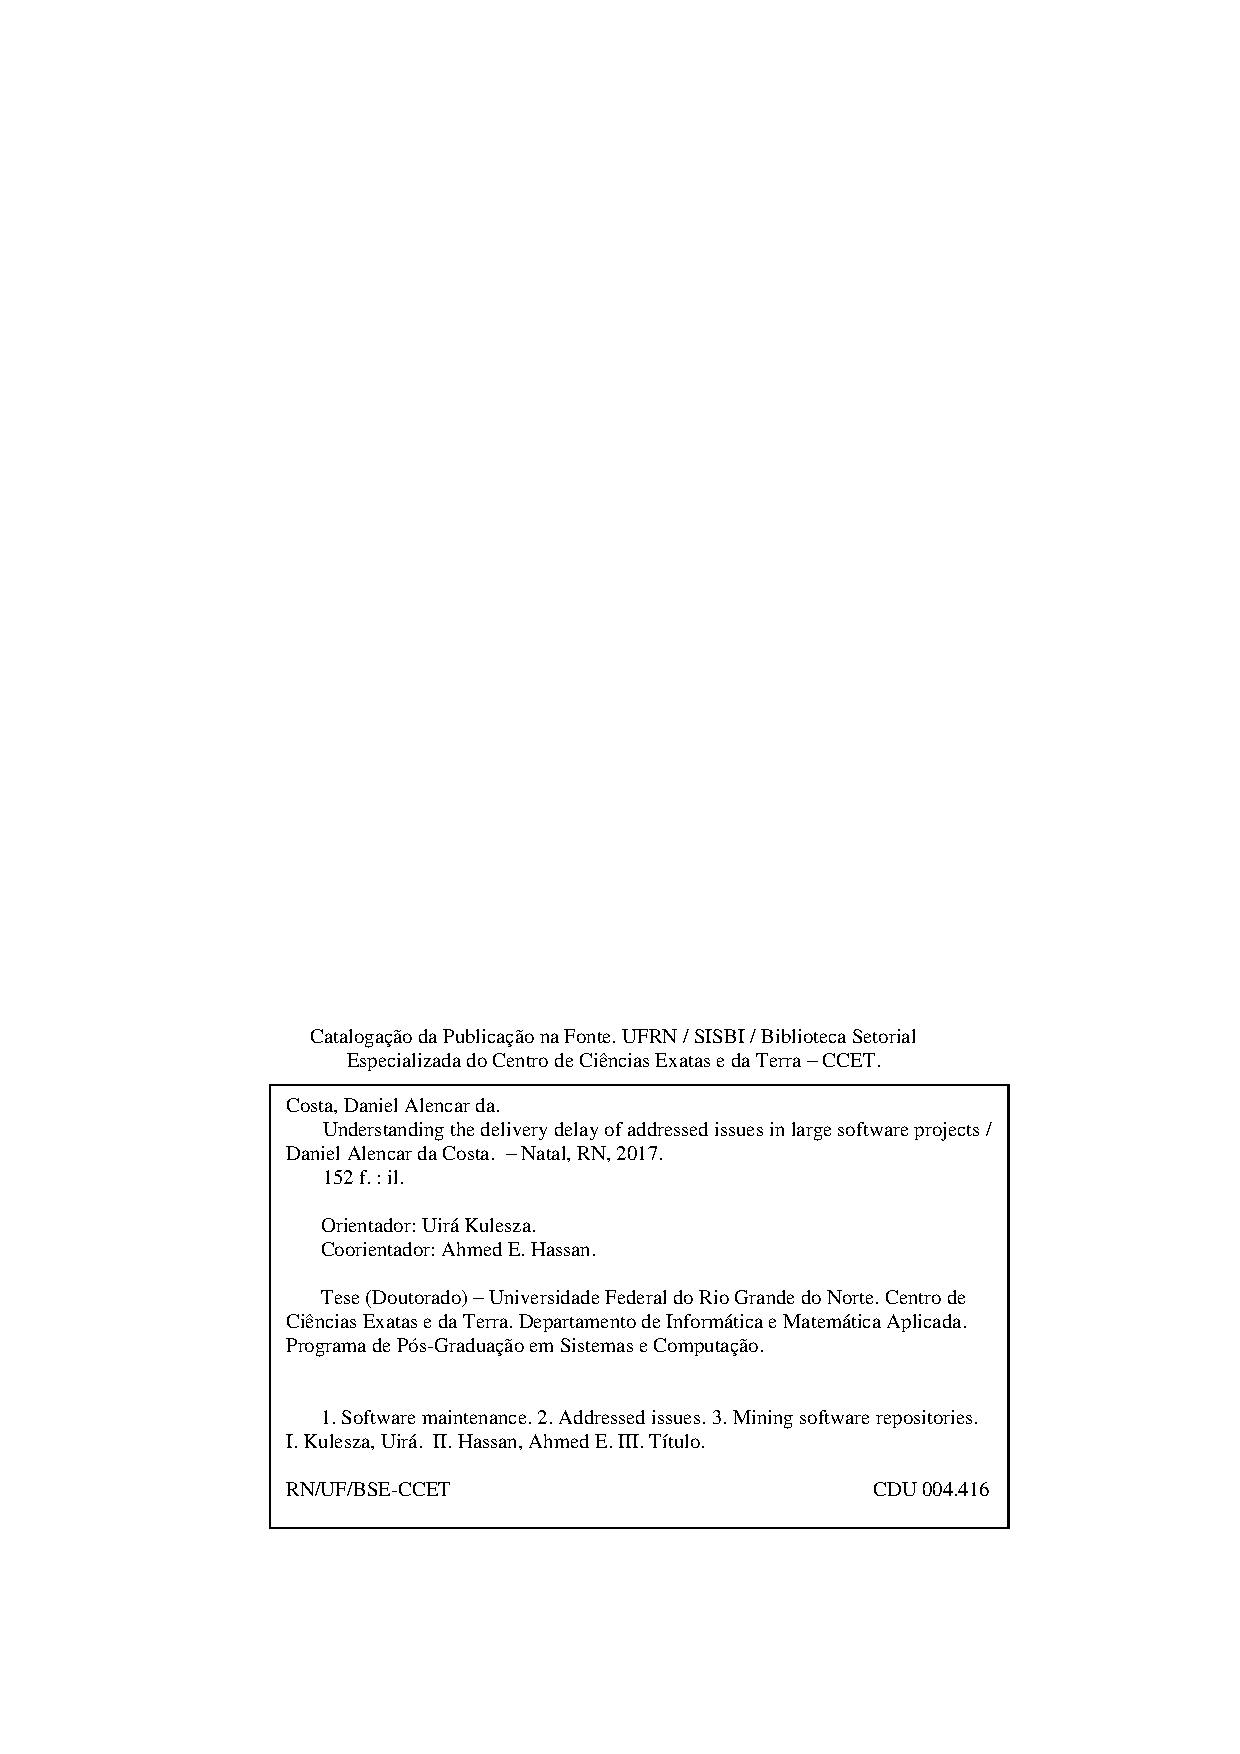
\includepdf{com_ficha_catalografica/ficha_catalografica.pdf}
%\begin{fichacatalografica}
%	\sffamily
%	\vspace*{\fill}					% Posição vertical
%	\begin{center}					% Minipage Centralizado
%	\fbox{\begin{minipage}[c][8cm]{13.5cm}		% Largura
%	\small
%	\imprimirautor
%	%Sobrenome, Nome do autor
%	
%	\hspace{0.5cm} \imprimirtitulo  / \imprimirautor. --
%	\imprimirlocal, \imprimirdata-
%	
%	\hspace{0.5cm} \pageref{LastPage} p. : il. (algumas color.) ; 30 cm.\\
%	
%	\hspace{0.5cm} \imprimirorientadorRotulo~\imprimirorientador\\
%	
%	\hspace{0.5cm}
%	\parbox[t]{\textwidth}{\imprimirtipotrabalho~--~\imprimirinstituicao,
%	\imprimirdata.}\\
%	
%	\hspace{0.5cm}
%		1. Integration Delay.
%		2. Empirical Study.
%		3. Mining Software Repository.
%		I. Uir\'{a} Kulesza.
%		II. Universidade Federal do Rio Grande do Norte.
%		III. Departamento de Inform\'{a}tica e Matem\'{a}tica Aplicada (DIMAp).
%		IV. Understanding the Delay to Deliver New Software Content
%	\end{minipage}}
%	\end{center}
%\end{fichacatalografica}
%% ---

%\begin{errata}
Elemento opcional da \citeonline[4.2.1.2]{NBR14724:2011}. Exemplo:

\vspace{\onelineskip}

FERRIGNO, C. R. A. \textbf{Tratamento de neoplasias ósseas apendiculares com
reimplantação de enxerto ósseo autólogo autoclavado associado ao plasma
rico em plaquetas}: estudo crítico na cirurgia de preservação de membro em
cães. 2011. 128 f. Tese (Livre-Docência) - Faculdade de Medicina Veterinária e
Zootecnia, Universidade de São Paulo, São Paulo, 2011.

\begin{table}[htb]
\center
\footnotesize
\begin{tabular}{|p{1.4cm}|p{1cm}|p{3cm}|p{3cm}|}
  \hline
   \textbf{Folha} & \textbf{Linha}  & \textbf{Onde se lê}  & \textbf{Leia-se}  \\
    \hline
    1 & 10 & auto-conclavo & autoconclavo\\
   \hline
\end{tabular}
\end{table}

\end{errata}


%\begin{folhadeaprovacao}

  \begin{center}
    {\ABNTEXchapterfont\large\imprimirautor}

    \vspace*{\fill}\vspace*{\fill}
    \begin{center}
      \ABNTEXchapterfont\bfseries\Large\imprimirtitulo
    \end{center}
    \vspace*{\fill}
    
    \hspace{.45\textwidth}
    \begin{minipage}{.5\textwidth}
        \imprimirpreambulo
    \end{minipage}%
    \vspace*{\fill}
   \end{center}
        
   Trabalho aprovado. \imprimirlocal, 24 de novembro de 2012:

   \assinatura{\textbf{\imprimirorientador} \\ Orientador} 
   \assinatura{\textbf{Professor} \\ Convidado 1}
   \assinatura{\textbf{Professor} \\ Convidado 2}
   %\assinatura{\textbf{Professor} \\ Convidado 3}
   %\assinatura{\textbf{Professor} \\ Convidado 4}
      
   \begin{center}
    \vspace*{0.5cm}
    {\large\imprimirlocal}
    \par
    {\large\imprimirdata}
    \vspace*{1cm}
  \end{center}
  
\end{folhadeaprovacao}


%% ---
% Dedicatória
% ---
\begin{dedicatoria}
   \vspace*{\fill}
   \centering
   \noindent
   \textit{My text here.} \vspace*{\fill}
\end{dedicatoria}
% ---


% ---
% Agradecimentos
% ---
\begin{agradecimentos}

	I belive that behind every scientific work there is an untold story that
	cannot be expressed by the methodologies, statistics and conclusions
	that are reported in the scientific papers. I dedicate this page to
	express my gratitude to some of the important pieces of my story.

	First and foremost, I would like to thank God for his blessings on every
	tiny step that was necessary to conceive this thesis. Among His
	blessings, I would like to start thanking my advisor Ahmed E. Hassan.
	Without his guidance and incentives, I would not be able to achieve the
	current state of this thesis. I would also like to thank my mentor and
	friend Shane McIntosh. His mentorship was fundamental to shape my work.
	I am also grateful to the co-authors of the publications that are
	directly and indirectly related to this thesis, Surafel Lemma Abebe,
	Weiyi Shang, Roberta Coelho, Christoph Treude, and Eduardo Aranha.
	Nevertheless, I could not have met these people without the support of
	my advisor and friend Uir\'{a} Kulesza, who always incentivized me to
	travel abroad and learn new skills. I am very grateful for his permanent
	support since my masters course.

	I am really grateful for my family, Danilo Alencar da Costa, Bruno
	Alencar da Costa, Carla Alencar da Costa, Maria Heliana Alencar da
	Costa, and Carlos Ara\'{u}jo da Costa. In my opinion, if one's mind is
	able to deeply focus on a problem that leads to a PhD thesis, its
	because there is a5lovely family on its background.

	I have had the privillege of meeting wonderful friends during my PhD
	journey, Mohamed Sami Rakha, Guilherme Gon\c{c}alves, Gabriel dos Anjos
	Cavalcanti, Tiago Targino, Hernani (Sanilton) Sarra Filho, and Suhas
	Kabinna. Their friendship was essential to make my PhD experience much
	more enjoyable.  The same holds for my older friendships, Allan Santos
	dos Santos---which I consider an extension of my family---and Thiago
	Reis da Silva. 

	Finally, I am thankful to my girlfriend Renata Sousa for always
	believing on me. She has the talent to make me see myself as a better
	man.

\end{agradecimentos}


%% ---
% Epígrafe
% ---
\begin{epigrafe}
    \vspace*{\fill}
	\begin{flushright}
		\textit{``Não vos amoldeis às estruturas deste mundo, \\
		mas transformai-vos pela renovação da mente, \\
		a fim de distinguir qual é a vontade de Deus: \\
		o que é bom, o que Lhe é agradável, o que é perfeito.\\
		(Bíblia Sagrada, Romanos 12, 2)}
	\end{flushright}
\end{epigrafe}
% ---


%% resumo em português
\setlength{\absparsep}{18pt} % ajusta o espaçamento dos parágrafos do resumo
\begin{resumo}
 Segundo a \citeonline[3.1-3.2]{NBR6028:2003}, o resumo deve ressaltar o
 objetivo, o método, os resultados e as conclusões do documento. A ordem e a extensão
 destes itens dependem do tipo de resumo (informativo ou indicativo) e do
 tratamento que cada item recebe no documento original. O resumo deve ser
 precedido da referência do documento, com exceção do resumo inserido no
 próprio documento. (\ldots) As palavras-chave devem figurar logo abaixo do
 resumo, antecedidas da expressão Palavras-chave:, separadas entre si por
 ponto e finalizadas também por ponto.

 \textbf{Palavras-chave}: latex. abntex. editoração de texto.
\end{resumo}


% resumo em inglês
\begin{resumo}[Abstract]
 \begin{otherlanguage*}{english}

	 The timely delivery of addressed software issues (i.e., bug fixes,
	 enhancements, and new features) is what drives software development.
	 Previous research has investigated what impacts the time to triage and
	 address (or fix) issues. Nevertheless, even though an issue is
	 addressed, \ie a solution is coded and tested, such an issue may still
	 suffer delay before being delivered to end users. Such delays are
	 frustrating, since end users care most about when an addressed issue is
	 available in the software system (i.e, released). In this matter, there
	 is a lack of empirical studies that investigate why addressed issues
	 take longer to be delivered compared to other issues. In this thesis,
	 we perform empirical studies to understand which factors are associated
	 with the delayed delivery of addressed issues. In our studies, we find
	 that 34\% to 98\% of the addressed issues of the ArgoUML, Eclipse and
	 Firefox projects have their integration delayed by at least one
	 release. Our explanatory models achieve ROC areas above 0.74 when
	 explaining delivery delay. We also find that the workload of
	 integrators and the moment at which an issue is addressed are the
	 factors with the strongest association with delivery delay.  We also
	 investigate the impact of rapid release cycles on the delivery delay of
	 addressed issues. Interestingly, we find that rapid release cycles of
	 Firefox are not related to faster delivery of addressed issues. Indeed,
	 although rapid release cycles address issues faster than traditional
	 ones, such addressed issues take longer to be delivered. Moreover, we find
	 that rapid releases deliver addressed issues more consistently than
	 traditional ones. Finally, we survey 37 developers of the ArgoUML,
	 Eclipse, and Firefox projects to understand why delivery delays occur.
	 We find that the allure of delivering addressed issues more quickly to
	 users is the most recurrent motivator of switching to a rapid release
	 cycle. Moreover, the possibility of improving the flexibility and quality of
	 addressed issues is another advantage that are perceived by our
	 participants. Additionally, the perceived reasons for the delivery
	 delay of addressed issues are related to decision making, team
	 collaboration, and risk management activities. Moreover, delivery delay
	 likely leads to user/developer frustration according to our
	 participants. Our thesis is the first work to study such an important
	 topic in modern software development. Our studies highlight the
	 complexity of delivering issues in a timely fashion (for instance,
	 simply switching to a rapid release cycle is not a silver bullet that
	 would guarantee the quicker delivery of addressed issues).

   \vspace{\onelineskip}
 
   \noindent 
   \textbf{Keywords}: Addressed Issues. Delivery Delay. Mining Software
   Sepositories. Software Maintenance.
 \end{otherlanguage*}
\end{resumo}


\pretextualchapter{Publications}
\begin{sloppypar}

\noindent Earlier versions of the work in this thesis were published as listed below:

\begin{itemize}

\item \textbf{Studying the Impact of Switching to a Rapid Release Cycle on
Integration Delay of Addressed Issues - An Empirical Study of the Mozilla
Firefox Project.} 
\underline{Daniel Alencar da
	Costa}, Shane McIntosh, Uir\'{a} Kulesza,
	and Ahmed E. Hassan. In Proceedings of the 13th International
Conference on Mining Software Repositories (MSR) , 2016, pp. 374--385.\\
\faTrophy {\em Received the ACM SIGSOFT distinguished paper award} \faTrophy

\item \textbf{An Empirical Study of Delays in the Integration of Addressed
Issues.} \underline{Daniel Alencar da Costa}, Shane McIntosh, Surafel Lemma Abebe,
Uir\'{a} Kulesza, and Ahmed E. Hassan. In Proceedings of the 30th International
Conference on Software Maintenance and Evolution (ICSME), 2014, pp. 281--290.\\
\faTrophy {\em Nominated for best paper award} \faTrophy

\end{itemize}

\noindent The following publications are not directly related to the work that
is presented in this thesis. Instead, they were produced in parallel to the
research performed in this thesis.

\begin{itemize}

\item \textbf{A Framework for Evaluating the Results of the SZZ Approach for
	Identifying Bug-Introducing Changes.} \underline{Daniel Alencar da
	Costa}, Shane McIntosh, Weiyi Shang, Uir\'{a} Kulesza, Roberta Coelho,
	and Ahmed E. Hassan. In the Transactions of Software Engineering Journal
	(TSE), 2016, 18 pages.

\item \textbf{How does the Shift to GitHub Impact Project Collaboration?} Luiz
	Felipe Dias, Igor Steinmacher, Gustavo Pinto, \underline{Daniel Alencar
	da Costa}, and Marco Gerosa. In the 32nd International Conference on
	Software Maintenance and Evolution (ICSME-ERA), 2016, 5 pages.

\item \textbf{Unveiling Developers Contributions Behind Code Commits: An
	Exploratory Study.} \underline{Daniel Alencar da Costa}, Uir\'{a} Kulesza, Eduardo Aranha,
	and Roberta Coelho. In Proceedings of the 29th Annual ACM Symposium on Applied
	Computing (SAC), 2014, pp. 1152--1157.

\item \textbf{Assessing and Evolving a Domain Specific Language for Formalizing Software
	Engineering Experiments: An Empirical Study.} Mar\'{i}lia Freire, Uir\'{a}
	Kulesza, Eduardo Aranha, Gustavo Nery, \underline{Daniel Alencar da Costa},
	Andreas Jedlitschka, Edmilson Campos, Silvia Acu\~{n}a, and Marta G\'{o}mez.
	International Journal of Software Engineering and Knowledge Engineering
	(IJSEKE), 2014, pp. 1509--1531.

\item 

\end{itemize}

\end{sloppypar}
\newpage


% ---
% inserir lista de ilustrações
% ---
\pdfbookmark[0]{\listfigurename}{lof}
\listoffigures*
\cleardoublepage
% ---


% ---
% inserir lista de tabelas
% ---
\pdfbookmark[0]{\listtablename}{lot}
\listoftables*
\cleardoublepage
% ---


%% ---
% inserir lista de abreviaturas e siglas
% ---
\begin{siglas}
  \item[ABNT] Associação Brasileira de Normas Técnicas
  \item[abnTeX] ABsurdas Normas para TeX
\end{siglas}
% ---


%% ---
% inserir lista de símbolos
% ---
\begin{simbolos}
  \item[$ \Gamma $] Letra grega Gama
  \item[$ \Lambda $] Lambda
  \item[$ \zeta $] Letra grega minúscula zeta
  \item[$ \in $] Pertence
\end{simbolos}
% ---


% ---
% inserir o sumario
% ---
\pdfbookmark[0]{\contentsname}{toc}
\tableofcontents*
\cleardoublepage
% ---


% ----------------------------------------------------------
% ELEMENTOS TEXTUAIS
% ----------------------------------------------------------
\textual

% ----------------------------------------------------------
% Introdução (exemplo de capítulo sem numeração, mas presente no Sumário)
% ----------------------------------------------------------
\chapter[Introduction]{Introduction}
%\addcontentsline{toc}{chapter}{Introduction}
% ----------------------------------------------------------

Attracting and retaining the interest of users are key factors for a software
system to achieve sustained
success~\cite{subramaniam2009determinants,delone2003delone}. In this context,
software development teams that do not address issues that are reported by
users, lead their software system to remain stagnant and lose credibility. We
broadly use the term issue to either describe a \textit{new feature}, a
\textit{bug}, or an \textit{enhancement} that should be addressed in a software
system~\cite{giuliano2008}.

Within a globalized world, in which technology has fostered geographically
distributed software development~\cite{herbsleb2003empirical}, software
development teams use \textit{Issue Tracking Systems} (ITS, e.g., Bugzilla) to
coordinate their tasks.\smartfoot{\url{https://www.bugzilla.org/}} Users can use
ITSs to report issues within software systems. To do so, these users must fill
in a report that contain information about the issue (\eg the description and
severity of the issue). 

The basic lifecycle of an issue is comprised of four steps. First, an issue is
{\em reported} to the software project's team. Once reported, an issue has to be
\textit{triaged}, \ie the team members must decide whether an issue should be
addressed or not. In case that an issue is deemed to be worth addressing, a team
member with the right expertise is assigned to the issue~\cite{Anvik2006}. After
being triaged, an issue is \textit{addressed} by its assignee, \ie a solution is
provided and tested for that issue. Finally, the addressed issue is integrated
and delivered to the end user through an official release of the software
system.  Issues may also be \textit{reopened} if the solution that was provided
to the issue is found to be incorrect. In this case, a new solution has to be
provided, tested, and integrated.

\section{Problem Statement} \label{sec:problem}

Once an issue is \textit{addressed}, (\ie a solution for that issue is provided
and tested), such an addressed issue may still have a delay before reaching users.
For instance, Jiang~\etal~\cite{Jiang2013} find that a reviewed code change
might take an additional 1-3 months to be integrated into the Linux kernel.
Users care most about when addressed issues will be available in the software
system (so they can benefit from those addressed issues). We use the term
\textit{delivery delay} to refer to the delay that addressed issues suffer prior
to their delivery to end users. 

Delivery delay can be frustrating to users. For example, in a recent issue
report of the Firefox system, a user asks: \textit{``So when does this stuff get
added? Will it be applied to the next FF23 beta? A 22.01 release?
Otherwise?''}.\smartfoot{\url{https://bugzilla.mozilla.org/show_bug.cgi?id=883554}}
Moreover, in the open source software community, developers may also be
motivated to contribute because they want to see a particular feature available
in the software system in a timely manner~\cite{Jiang2013}. In such a case,
delivery delays frustrate these contributors. 

The present thesis is an effort to reduce the lack of empirical understanding as
to why addressed issues suffer delivery delay before being available to users. A
good understanding of such delays will help software projects reduce such
undesirable delays.

\section{Current Research Limitations}

Prior research has investigated the time that is needed to triage and address
issues~\cite{Anvik2005, Anbalagan2009, Giger2010, Kim2006, Marks2011, Weib2007,
Zhang2013}. Such research provides valuable insight on which issues should be
prioritized. For example, issues might be addressed earlier given the estimated
time that they are likely to take to be addressed. Nevertheless, after an issue
is addressed, such an addressed issue may still require considerable time to be
delivered to users.

Another line of prior work has investigated the integration stage of software
development. Jiang~\etal~\cite{Jiang2013} studied the likelihood of patches that
were submitted to the Linux Kernel project of being integrated in the main code
base. On the other hand,
Choetkiertikul~\etal~\cite{riskyissues2015a,riskyissues2015b} studied the risk
of issues of postponing the shipment of new releases. However, the investigation
of: {\em (i)} what leads addressed issues to suffer delivery delay even when
releases are shipped and {\em (ii)} the impact of release development strategies
on such delays remain as open challenges.

\section{Thesis Proposal} \label{sec:thesis_overview}

\begin{sloppypar}
The general research question that is investigated in this thesis is {\em
\underline{what leads addressed issues to suffer delivery delay?}}
\end{sloppypar}

\begin{figure}[t]
	\centering
	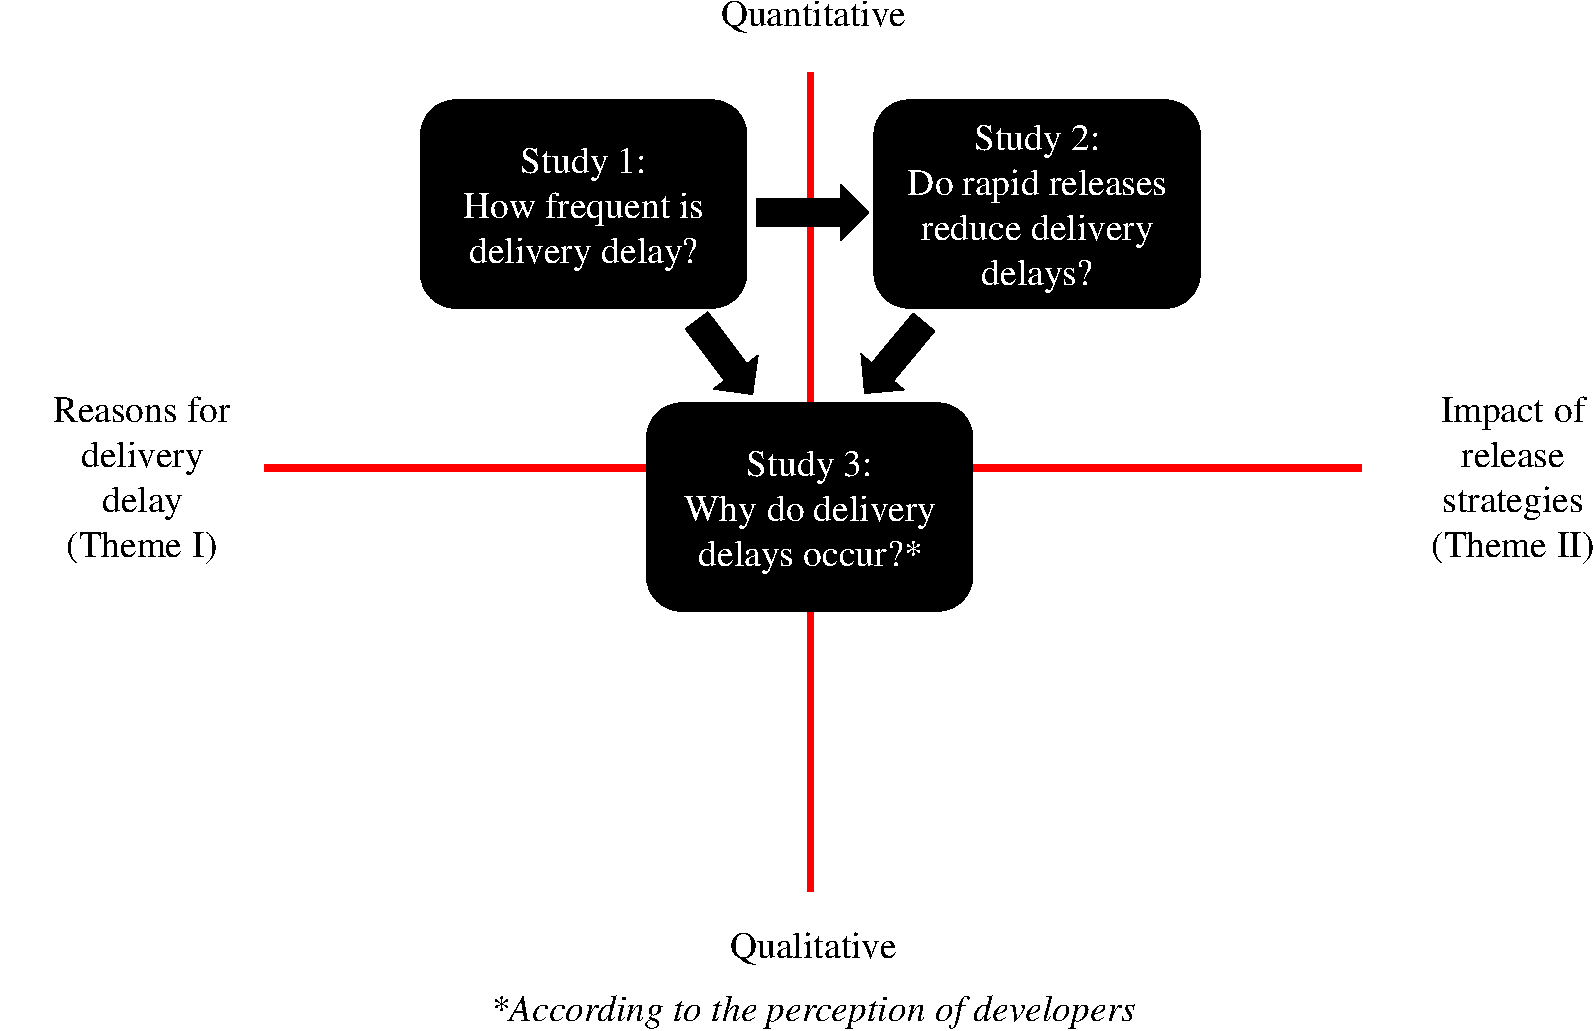
\includegraphics[width=0.90\textwidth,keepaspectratio]
	{chapters/chapter1/figures/thesis_overview.pdf}
	\caption{An overview of the scope of the thesis.}
	\label{fig:thesis_overview}
\end{figure}

\hyperref[fig:thesis_overview]{Figure}~\ref{fig:thesis_overview} provides an
overview of the scope of this thesis. The scope shows the studies that we
perform towards our general research question. The studies that are performed in
this thesis are grouped into two {\em themes}. {\em
Theme~I}\parts{pt:deliverydelay} is regarding {\em reasons for delivery delay},
which encompasses \hyperref[st:study1]{Studies}~\ref{st:study1} and part of
\hyperref[st:study4]{Study}~\ref{st:study4}. In {\em
Theme~II}\parts{pt:rapidreleases}, we investigate the {\em impact of release
development strategies} on the delivery delay of addressed issues
(\hyperref[st:study3]{Study}~\ref{st:study3} and part of
\hyperref[st:study4]{Study}~\ref{st:study4}). We present the motivation for
conducting each study of this thesis in the subsections below.

\subsection{Study~1---How frequent is delivery delay?}

\study{st:study1} 33\% of the code patches that are submitted to resolve issues
of the Linux kernel take 3 to 6 months to be accepted into an official
release~\cite{Jiang2013}. Such observation hints that the integration stage may
introduce non-trivial delays before delivering addressed issues. Since there is
a lack of empirical studies that investigate the frequency of delivery delays of
addressed issues, we perform a study using 20,995 addressed issues of the
ArgoUML, Eclipse, and Firefox projects in
\hyperref[st:study1]{Study}~\ref{st:study1}. Our main goal is to analyze {\em
(i)} how frequent delivery delays occur and {\em (ii)} which factors may impact
delivery delay according to our studied data.
%\subsection{Study~2---What leads to prolonged delivery delays?}
%\study{st:study2} 

Also in this study, we investigate delivery delays that are considered to be
{\em prolonged} in a particular project. For example, supposing that addressed
issues are usually delivered within 60 days on a particular project, a delivery
delay of 120 days would be abnormal for that project. This investigation is
important because prolonged delays can be more frustrating to users, since they
are not used to such delays.

%This was the first study that was conducted for this thesis, since we were
%interested on investigating  how frequent and how long are the delivery delays
%of addressed issues. In this study we use a quantitative approach for measuring
%the frequency of delivery delays.

\subsection{Study~2---Do rapid releases reduce delivery delays?}

\study{st:study3} After an issue is addressed, a release must be shipped in
order to end users experience the addressed issue. The process of shipping
releases varies according to the release cycles that are adopted by the project
team. Recently, many organizations have shifted to shorter release cycles (\eg
6 weeks rather than 12 months) with the allure of delivering software issues
more quickly to end users. For instance, Firefox, Chrome, and Facebook have
adopted shorter release cycles to ship major releases. In
\hyperref[st:study3]{Study}~\ref{st:study3}, we empirically study whether
shorter release cycles quicken the delivery of addressed issues to end users. We
set out to empirically compare the traditional and rapid releases of the Firefox
project regarding the delivery delay of addressed issues. In total, we study 71,114
issue reports.

\subsection{Study~3---Why do delivery delays occur?}

\study{st:study4} In our other studies
(\hyperref[st:study1]{Studies}~\ref{st:study1} and \ref{st:study3}), we
quantitatively investigate the delivery delay of addressed issues. We perform
several statistical analyses based on the data that is publicly available on the
ITSs and {\em Version Control Systems} (VCSs) of our subject projects. Nevertheless, to better understand the
reasons as to why delivery delays occur, we survey 37 participants from the
ArgoUML, Firefox, and Eclipse projects about the delivery delay of addressed
issues. We also perform follow up interviews with four participants to get
deeper insights about the responses that we receive.
\hyperref[st:study4]{Study}~\ref{st:study4} help us to {\em (i)} reach
additional insights that could not be possible by only performing quantitative
analysis and {\em (ii)} verify whether our participants agree with our
findings from the quantitative studies. 

\subsection{Chronology of Studies}

The arrows in \hyperref[fig:thesis_overview]{Figure}~\ref{fig:thesis_overview}
describe which studies inspired the others.
\hyperref[st:study1]{Study}~\ref{st:study1} was the first to be conducted in
this thesis, since we were interested on investigating how frequent and long are
the delivery delays of addressed issues. After conducting
\hyperref[st:study1]{Study}~\ref{st:study1}, we observed a considerable
difference between the rapidly released Firefox and the other two studied
projects (\ie Eclipse and ArgoUML) regarding the frequency of delivery delays.
In our second study (\hyperref[st:study3]{Study}~\ref{st:study3}), we extended
our Firefox dataset in order to compare the traditional and rapid releases
regarding delivery delays. Such an investigation helps us on better
understanding whether rapid releases may decrease delivery delays in terms of
days. Finally, both studies motivated us to perform
\hyperref[st:study4]{Study}~\ref{st:study4}. We use mixed methods to perform our
studies. As shown in
\hyperref[fig:thesis_overview]{Figure}~\ref{fig:thesis_overview}, we use
quantitative analyses in \hyperref[st:study1]{Studies}~\ref{st:study1}
and~\ref{st:study3} (\ie statistics and machine learning techniques). On the
other hand, \hyperref[st:study4]{Study}~\ref{st:study4} is mainly qualitative,
\ie we use surveys and interviews to obtain our data (although we perform some
quantitative analysis as well).

\section{Thesis Contributions}

We outline the contributions of this thesis below. The contributions are grouped
by their respective study.

\subsubsection*{Study~1---How frequent is delivery delay?}

\begin{itemize}

	\item Despite being addressed well before an upcoming release, 34\% to
		60\% of the addressed issues are not integrated in more than one
		release in the ArgoUML and Eclipse projects. Furthermore, 98\%
		of the Firefox project issues had their delivery delayed by
		at least one release
		(\hyperref[ch:study12]{Chapter}~\ref{ch:study12}).

	\item Heuristics that estimate the effort that teams invest in
		fixing issues are the most influential factors to
		estimate delivery delay in terms of number of releases
		(\hyperref[ch:study12]{Chapter}~\ref{ch:study12}).

	\item Surprisingly, \textit{priority} and \textit{severity} have little
		impact on delivery delay. Indeed, 36\% to 97\% of priority P1
		addressed issues were delayed by at least one release
		(\hyperref[ch:study12]{Chapter}~\ref{ch:study12}).

	\item Shorter delivery delays are associated with issues that are
		addressed during more controlled stages (\eg a code freeze
		stage) of a given release cycle
		(\hyperref[ch:study12]{Chapter}~\ref{ch:study12}).

	\item The time at which issues are addressed and the resolvers
		of the issues have great impact on estimating the
		delivery delay (in terms of days) of an issue
		(\hyperref[ch:study12]{Chapter}~\ref{ch:study12}).

	\item The time at which an issue is addressed (queue position), the
		integration workload (in terms of the backlog of addressed
		issues), and the heuristics that estimate the effort that teams
		invest in fixing issues (fixing time per resolver), are the most
		influential attributes for issues that have a prolonged delivery
		delay (\hyperref[ch:study12]{Chapter}~\ref{ch:study12}). 

	\item Our models that identify addressed issues that have a prolonged
		delivery delay outperform random guessing and Zero-R models,
		obtaining AUC values of 0.82~to~0.96
		(\hyperref[ch:study12]{Chapter}~\ref{ch:study12}).

\end{itemize}

\subsubsection*{Study~2---Do rapid releases reduce delivery delays?}

\begin{itemize}

	\item Although issues tend to be addressed more quickly in rapid
		release cycles, addressed issues tend to be integrated into
		consumer-visible releases more quickly in traditional
		release cycles. However, a rapid release cycle may improve the
		consistency of the delivery rate of addressed issues
		(\hyperref[ch:study34]{Chapter}~\ref{ch:study34}).

	\item The total time that is spent from the issue report date to its
		delivery into a release is not significantly different
		between traditional and rapid releases
		(\hyperref[ch:study34]{Chapter}~\ref{ch:study34}).

	\item In traditional releases, addressed issues are less likely to be
		delayed if they are addressed recently in the backlog. On the
		other hand, in rapid releases, addressed issues are less likely
		to be delayed if they are addressed recently in the current
		release cycle (\hyperref[ch:study34]{Chapter}~\ref{ch:study34}). 
\end{itemize}

\subsubsection*{Study~3---Why do delivery delays occur?}

\begin{itemize}

	\item The perceived reasons for delivery delay of addressed issues are
		primarily related to activities such as development, decision
		making, team collaboration, and risk management
		(\hyperref[ch:study34]{Chapter}~\ref{ch:study34}). 

	\item  The dependency of issues on other projects and team workload are the main
		perceived reasons to explain our data about delivery delay in
		general (\hyperref[ch:study34]{Chapter}~\ref{ch:study34}).  

	\item The allure of delivering addressed issues more quickly to users is
		the most recurrent motivator for switching to a rapid release
		cycle. In addition, the allure of improving management
		flexibility and quality of addressed issues are other advantages
		of rapid releases that are perceived by our participants
		(\hyperref[ch:study34]{Chapter}~\ref{ch:study34}).

	\item Integration rush and the increased time that is spent on polishing
		addressed issues (during rapid releases) emerge as one of the
		main explanations as to why traditional releases may have
		shorter delivery delays.
		(\hyperref[ch:study34]{Chapter}~\ref{ch:study34}).

\end{itemize}

\section{Thesis Organization}

The remainder of this thesis is organized as follows. In
\hyperref[ch:background]{Chapter}~\ref{ch:background}, we provide the background
material to the reader. In \hyperref[ch:study12]{Chapter}~\ref{ch:study12},
\hyperref[ch:study34]{Chapter}~\ref{ch:study34}, and
\hyperref[chapter6]{Chapter}~\ref{chapter6}, we present
\hyperref[st:study1]{Studies}~\ref{st:study1},~\ref{st:study3},
and~\ref{st:study4}, respectively. In
\hyperref[chapter7]{Chapter}~\ref{chapter7}, we present related research with
respect to this thesis. Finally, in
\hyperref[ch:conclusions]{Chapter}~\ref{ch:conclusions}, we draw our
conclusions.


\chapter[Background]{Background} \label{ch:background}

In this chapter, we describe the key concepts that are necessary to understand
the studies that are performed in this thesis.

\section{Issue Reports}

One of the main factors that drives software evolution is the issues that are
filed by users, developers, and quality assurance personnel. Below, we describe
what issues are and the major steps involved in addressing and integrating them.

We use the term {\em issue} to broadly refer to bug reports, enhancements, and
new feature requests~\cite{giuliano2008}.  Issues can be filed by users,
developers, or quality assurance personnel. To track development progress,
software teams may use an ITS such as
Bugzilla\smartfoot{\url{https://www.bugzilla.org}} or
JIRA.\smartfoot{\url{https://www.atlassian.com/software/jira}} Such ITSs allow
for describing and monitoring the state of the issue reports.

Each issue in an ITS has a unique identifier, a brief description of the nature
of the issue, and a variety of other meta-data. Large software projects receive
plenty of issue reports on a daily basis. For example, the Eclipse and Firefox
projects respectively received an average of 65 and 89 issue reports daily (from
January to October 2016) on their
ITSs.\smartfoot{\url{https://bugs.eclipse.org/bugs}}$^,$\smartfoot{\url{https://bugzilla.mozilla.org/}}
The number of filed issues is usually greater than the size of the development
team. 

\begin{figure}[t]
	\centering
	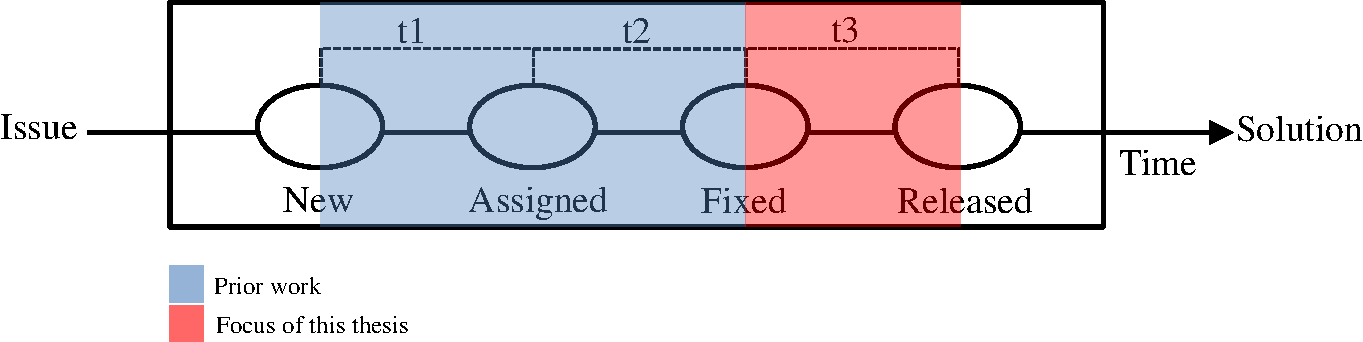
\includegraphics[width=\textwidth,keepaspectratio]
	{chapters/chapter2/figures/issue_lifecycle.pdf}
	\caption{An overview of an issue's life cycle.}
	\label{fig:issue_lifecycle2}
\end{figure}

\hyperref[fig:issue_lifecycle2]{Figure}~\ref{fig:issue_lifecycle2} shows the
stages of an issue's life cycle. After an issue has been filed, project managers
and team leaders {\em triage} them, \ie assign them to developers, denoting the
urgency of the issue using priority and severity fields~\cite{Anvik2006} (time
{\em t1} of \hyperref[fig:issue_lifecycle2]{Figure}~\ref{fig:issue_lifecycle2}). 

After being triaged, issues are then {\em addressed} (or {\em fixed} in case of
bugs), \ie solutions to the described issues are provided by developers (time
{\em t2} of \hyperref[fig:issue_lifecycle2]{Figure}~\ref{fig:issue_lifecycle2}).  Generally speaking, an issue may be in an open or closed state.  An
issue is marked as open when a solution has not yet been found. We consider
UNCONFIRMED, CONFIRMED, and IN\_PROGRESS as open states. An issue is considered
closed when a solution has been found. 

Usually, a \textit{resolution} is provided with a closed issue. For instance, if
a developer made code changes to address an issue, the state and resolution
combination should be RESOLVED-FIXED.  However, if the developer was not able to
reproduce the bug, then the state and resolution may be
RESOLVED-WORKSFORME.\smartfoot{\url{https://bugzilla.mozilla.org/page.cgi?id=fields.html}}

Finally, addressed issues must be integrated into an official release (\ie
releases that are intended for end users) in order to make them available (time
{\em t3} of \hyperref[fig:issue_lifecycle2]{Figure}~\ref{fig:issue_lifecycle2}),
which is the life cycle stage that is mainly studied in this thesis.  The life
cycle of issues is documented in detail on the Bugzilla
website.\smartfoot{\url{https://bugzilla.readthedocs.org/en/5.0/using/editing.html\#life-cycle-of-a-bug}}
In the next sections, we describe the stages of the life cycle of an issue.

\conclusionbox{Prior work studied the triaging and fixing time of issues (blue
	color in
	\hyperref[fig:issue_lifecycle2]{Figure}~\ref{fig:issue_lifecycle2}). The
	focus of this thesis is the study of the delivery delay (red color in
	\hyperref[fig:issue_lifecycle2]{Figure}~\ref{fig:issue_lifecycle2}),
which is the needed time to deliver issues that are already addressed.}

\section{Triaging Issues}

{\em Issue triaging} is the process of deciding which issues have to be
addressed and assigning the appropriate developer to them \cite{Anvik2006}. This
decision depends of several factors, such as the impact of the issue on the
software or how much effort is required to address the issue.  Projects receive
a high number of issue reports, which is usually larger than the developer team.
Hence, effective triaging of issue reports is an important means of keeping up
with user demands. 

Hooimeijer and Weimer \cite{Hooimeijer2007} built a model to classify whether or
not an issue report will be ``cheap'' or ``expensive'' to triage by measuring
the quality of the report. Based on their findings, the authors state that the
effort required to maintain a software system could be reduced by filtering out
reports that are ``expensive'' to triage. Saha \etal \cite{Saha2014} studied
long lived issues, \ie issues that were not addressed for more than one year.
They found that the time to assign a developer and address such issues is
approximately two years. Our research complements these prior studies by
investigating the time that is necessary to deliver addressed issues 
rather than the time that is necessary to triage issues.

\section{Addressing Issues}
Once an issue is properly triaged, the assigned developer starts to address it.
To estimate the required time
to address issues, some approaches used the similarity of an issue report to
prior issue reports~\cite{Weib2007,Zhang2013}, while others built prediction models using different machine learning
techniques~\cite{Panjer2007,Anbalagan2009,Giger2010, Marks2011}. 

Kim and Whitehead~\cite{Kim2006} computed the time that was necessary to address
issues in ArgoUML and PostgreSQL. They found that the median issue fixing time
is about 200 days. Guo \etal~\cite{Guo2010} used logistic regression model to
predict the probability that a new issue will be fixed. The authors trained the
model on Windows Vista issues and achieved a precision of 0.68 and recall of
0.64 when predicting Windows 7 issue reports. These approaches focus on
estimating the required time to address an issue. In our studies, however, we
investigate the required time to deliver issues that are already addressed.

Recent empirical studies assess the relationship between the attributes that are
used to build prediction models for estimating the fixing time of issues.
Bhattacharya and Neamtiu \cite{Bhattacharya2011} performed univariate and
multivariate regression analyses to capture the significance of four attributes
in issue reports.  Their results indicate that more independent variables are
required to build better prediction models. 

Herraiz \etal~\cite{Herraiz2008} studied the mean time to close issues that were
reported to the Eclipse project and how severity and priority levels of the
issues affect such a time. In their study, the authors used one way analysis of
variance to group the different priority and severity levels that were used in
the issue reports of the Eclipse project. Based on their results, the authors
suggest the reduction of the currently used severity and priority levels to
three levels. 

Zhang \etal \cite{Zhang2012} investigated the delays incurred by developers in
the issue addressing process. The authors extract the duration of an issue (\ie
from open to closed) using interaction logs. The authors investigated the impact
of three dimensions of attributes that are related to issues: issue report
characteristics, source code, and code changes. The authors found that
attributes such as severity, operating system, issue description, and number of
comments are likely to impact the needed time to start addressing an issue as
well as the needed time to resolve an issue. 

As Zhang \etal \cite{Zhang2012}, we use attributes that are related to issue
reports to build explanatory models.  Nevertheless, our goal is to study
attributes that share a relationship with the needed time to deliver addressed
issues. We also investigate the impact that severity and priority levels have on
the delivery delay of addressed issues. 

\section{Integrating Issues} 

After issues are addressed, they need to be integrated into an official release,
so users can be benefited from them. Usually, user-intended releases are shipped
along with release notes, which are documents that specify what was added,
changed, or removed in such new
releases.\smartfoot{\url{https://www.mozilla.org/en-US/firefox/releases/}} Prior
research has studied the integration of addressed issues.
Jiang~\etal~\cite{Jiang2013} studied the integration process of the Linux
kernel. They found that 33\% of code patches that were submitted to resolve
issues are accepted into an official Linux release after 3 to 6 months.
Choetkiertikul~\etal~\cite{riskyissues2015a,riskyissues2015b} studied the risk
of issues introducing delays to deliver new releases of a software project.  In
this thesis, our focus is on the time that is required to deliver addressed
issues rather than the process of patches acceptance or the risk of a release
schedule slippage.

\section{Delivery Delay}\label{ch2:deliverydelay}

{\em Delivery delay} refers to the time between the moment at which an issue is
addressed (\ie changed to the RESOLVED-FIXED status) to the time at which such
an addressed issue is shipped to end users. In 
\hyperref[st:study1]{Studies}~\ref{st:study1} and~\ref{st:study3}, we analyze
two {\em dimensions} of delivery delay. The first dimension is comprised of two
types of delivery delay, which are: {\em (i)} delivery delay in terms of number
of releases and {\em (ii)} delivery delay in terms of days. As for the second
dimension, we study the {\em (iii)} prolonged delivery delays.

\begin{figure}
	\centering
	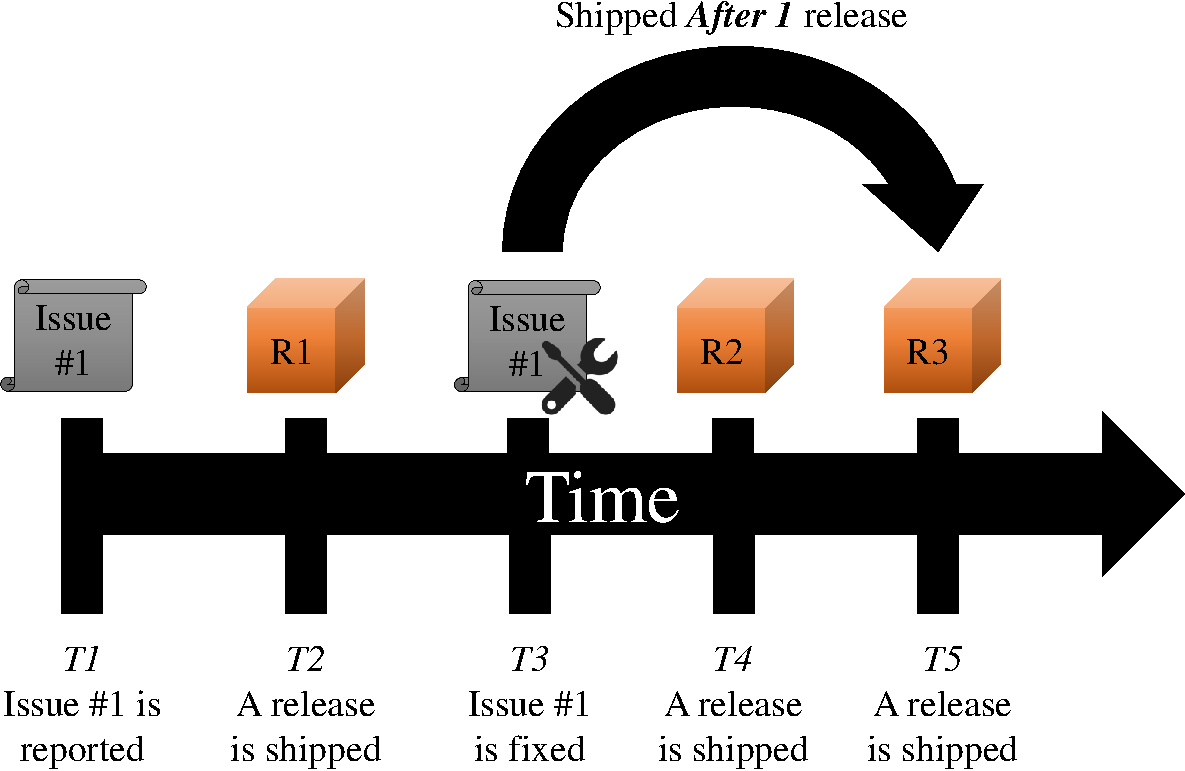
\includegraphics[width=.80\textwidth,keepaspectratio]
	{chapters/chapter2/figures/integration_delay_releases.pdf}
	\caption{An illustrative example of how we compute delivery delays.}
	\label{fig:integration_delay_releases}
\end{figure}

\mydef{Delivery delay in terms of releases}{def:1}
\hyperref[fig:integration_delay_releases]{Figure}
\ref{fig:integration_delay_releases} provides an example of how we measure
delivery delay. To compute the delivery delay in terms of number of releases, we
count the number of releases that a given fixed issue is prevented from
delivery. In
\hyperref[fig:integration_delay_releases]{Figure}~\ref{fig:integration_delay_releases},
Issue~\#1 is reported at time~{\em $t_1$}, fixed at~{\em $t_3$}, and shipped at
time~{\em $t_5$}. The delivery delay in terms of releases for Issue \#1 is the
number of official releases that are shipped between {\em $t_3$} and {\em
$t_5$}. Therefore, Issue~\#1 has a delivery delay of one release. 

\mydef{Delivery delay in terms of days}{def:2} We compute delivery delay in
terms of days using an approach that is similar
to~\hyperref[def:1]{Definition}~\ref{def:1}. However, instead of counting the
number of official releases, we count the number of days between {$t_3$} and
{$t_5$} (see
\hyperref[fig:integration_delay_releases]{Figure}~\ref{fig:integration_delay_releases}).
For instance, if the number of days between $t_i$ and $t_{(i+1)}$ in
\hyperref[fig:integration_delay_releases]{Figure}~\ref{fig:integration_delay_releases}
is 30 days, the delivery delay of issue~\#1 would be 60 days.

\mydef{Prolonged delivery delay}{def:3} Prolonged delivery delay occurs when the
delivery delay in terms of days (see \hyperref[def:2]{Definition}~\ref{def:2})
for a given addressed issue is above one {\em Median Absolute Deviation} (MAD)
of the median delivery delay of a studied project. MAD is the median of the
\textit{absolute deviations} from one distribution's median. The higher the MAD,
the greater is the variation of a distribution with respect to its
median~\cite{howell2005median,leys2013detecting}.

\section{Release Cycles} \label{subsec:firefox_releases}

A {\em release cycle} is the time period that is required by the development
team to develop and deliver a new release to end users. These releases could be
made available every few weeks or months, depending on the project release
policy. Releasing every few weeks is typically referred to as a \textit{rapid
release} cycle, while releasing monthly or yearly is typically referred to as a
\textit{traditional release} cycle~\cite{Mantyla2013}.

In our studies, we consider a release cycle length in the scale of days or weeks
as a {\em rapid} release cycle. For example, the release cycle of the Firefox
project is currently 6
weeks.\smartfoot{\url{https://wiki.mozilla.org/Release_Management/Release_Process}}
On the other hand, we consider a release cycle length of  several months or
years (\eg 12-18 months) as a traditional release cycle. In
\hyperref[st:study3]{Study}~\ref{st:study3}, we study the impact of adopting a
rapid release cycle on the delivery delay of addressed issues.

\section{Chapter Summary}

In this chapter, we provide the key concepts that we use in our studies to the
reader. We first present the concept of an {\em issue report}, which can either
represent an enhancement, a new feature, or a bug that has to be addressed in a
given project. Next, we describe the life cycle of an issue, which is basically
comprised of the {\em triaging}, {\em addressing}, and {\em integration} stages.
We then define the various types of {\em delivery delay} that we study in this
thesis. Finally, we describe the two types of release cycles that are
investigated in this thesis, which are the {\em rapid} and {\em traditional}
release cycles.


%\chapter[Related Research]{Related Research} \label{ch:relatedwork}

In the studies that we perform in this thesis, we investigate the delays that are related to the
delivery of new software content to end users. We also investigate if such delays are related to the
release cycle strategies that are adopted by the development team. Therefore, in the following
sections we describe the related research about the management of issues (\ie triaging, addressing,
and integration of issues) and the comparison between rapid and traditional release cycles in
software engineering.

\section{Triaging Issues}
To \textit{triage} issues is the process of deciding which issues have to be addressed and assigning
the appropriate developer to them \cite{Anvik2006}. This decision depends of several factors, such
as the impact of the issue on the software, or how much effort is required to address the issue.
Projects receive a high number of issue reports, which is usually larger than the developer team.
Hence, effective triaging of issue reports is an important means of keeping up with user demands. 

Hooimeijer and Weimer \cite{Hooimeijer2007} built a model to classify whether or not an issue report
will be ``cheap'' or ``expensive'' to triage by measuring the quality of the report. Based on their
findings, the authors state that the effort required to maintain a software system could be reduced
by filtering out reports that are ``expensive'' to triage. Saha \etal \cite{Saha2014} studied long
lived issues, \ie issues that were not addressed for more than one year. They found that the time to
assign a developer and address such issues is approximately two years. Our research
(Chapters~\ref{ch:integrationdelay}~and~\ref{ch:rapidvstrad}) complements these prior studies by
investigating the time to integrate issues once they are addressed rather than the time to assign a
developer to handle the issue.

\section{Addressing Issues}
Once an issue is properly triaged, the assigned developer starts to address it. To estimate the time
required to address issues, some approaches used the similarity of an issue to existing issues
\cite{Weib2007,Zhang2013}, while others built prediction models using different machine learning
techniques \cite{Panjer2007,Anbalagan2009,Giger2010, Marks2011}. 

Kim and Whitehead~\cite{Kim2006} computed the time taken to address issues in ArgoUML and
PostgreSQL. They found that the median issue-fix time is about 200 days. Guo \etal~\cite{Guo2010}
used logistic regression model to predict the probability that an new issue will be fixed. The
authors trained the model on Windows Vista issues and achieved a precision of 0.68 and recall of
0.64 when predicting Windows 7 issue reports. These approaches focus on estimating the time required
to address an issue. In our studies (Chapters~\ref{ch:integrationdelay}), however, we investigate in
which release an addressed issue will be integrated. 

Recent empirical studies assess the relationship between the attributes used to build models for
estimating bug fix time. Bhattacharya and Neamtiu \cite{Bhattacharya2011} performed univariate and
multivariate regression analyses to capture the significance of four features in issue reports.
Their results indicate that more independent variables are required to build better prediction
models. 

Herraiz \etal~\cite{Herraiz2008} studied the mean time to close issues reported in Eclipse, and how
the severity and priority levels of the issues affect this time. In their study, the authors used
one way analysis of variance to group the different priority and severity levels used in Eclipse.
Based on their result, the authors suggest to reduce the severity and priority options to three
levels. 

Zhang \etal \cite{Zhang2012} investigated the delays incurred by developers in the issue addressing
process. To do such analyses, they extract the beginning and ending time of an issue 
from interaction logs. The authors investigated the impact of three dimensions related to
issues: issue reports, source code involved in the issue, and code changes that are required to
address the issue. They found that metrics such as severity, operating system, description of the
issue, and comments are likely to impact the delays in starting to address the issue and changing
the status to RESOLVED. 

As Zhang \etal \cite{Zhang2012}, we use attributes related to issue reports to build explanatory
models (Chapters~\ref{ch:integrationdelay}~and~\ref{ch:rapidvstrad}). However, our aim is to
understand which attributes play an important role in the delay of integrating addressed issues.  In
addition, we investigate why severity and priority levels are not relevant to distinguish issue
reports that are addressed and integrated in a release prior to others.

\section{Integrating Issues} 

Prior research has studied delays related to the integration and delivery of addressed issues to end
users. Jiang~\etal~\cite{Jiang2013} studied the integration process of the Linux kernel. They found
that 33\% of the code patches that were submitted to resolve issues are accepted into an official
Linux release after 3 to 6 months. In Chapter~\ref{ch:integrationdelay}, we find that although
issues are addressed well before an upcoming release they may still be delayed. Indeed, 98\% of
addressed issues in the Firefox system were delayed by at least one release.
Choetkiertikul~\etal~\cite{riskyissues2015a,riskyissues2015b} study the risk of issues introducing
delays to deliver new releases of a software project.  

The integration of addressed issues is costly. Rahman~and~Rigby~\cite{rahmanrelease} found that the
period to stabilize addressed issues can take from 45 to 93 days in the Linux kernel and from 56 to
149 days in Chrome. Jiang~\etal~\cite{jiangmuch} proposes the ISOMO model to measure the cost of
integrating a new patch into a host project. 

Similar to Jiang \etal\cite{Jiang2013}, we also investigate the integration of addressed issues.
However, we focus on the integration delay of issues that have been addressed and not if a patch is
more likely to be accepted than the others
(Chapters~\ref{ch:integrationdelay}~and~\ref{ch:rapidvstrad}). 

Differently from Rahman~and~Rigby~\cite{rahmanrelease} and
Choetkiertikul~\etal~\cite{riskyissues2015a,riskyissues2015b}, the focus of our research is on the
time to deliver new content to end users rather than analyzing the time to stabilize issues or the
risk that a particular issue may cause on a release to be delayed.  Also, our work complements the
aforementioned studies by investigating the impact that the adoption of a rapid release cycle may
have upon the integration delay of addressed issues (Chapter~\ref{ch:rapidvstrad}).

\section{Traditional vs. Rapid Releases}

Shifting from traditional releases to rapid releases has been shown to have an impact on software
quality and quality assurance activities. M\"antyl\"a~\etal~\cite{mantyla2014rapid} found that rapid
releases have more tests executed per day but with less coverage. The authors also found that the
number of testers decreased in rapid releases, which increased the test workload.
Souza~\etal~\cite{souza2014rapid} found that the number of reopened bugs increased by 7\% when
Firefox changed to a rapid release cycle. Souza~\etal~\cite{souzabackout} found that backout of
commits increased when rapid releases were adopted.  However, they note that such results may be due
to changes in the development process rather than the rapid release cycle --- the backout culture
was not widely adopted during the Firefox traditional releases.

It is not clear yet if rapid releases lead to faster fixing of bugs.
Baysal~\etal~\cite{baysal2011tale} found that bugs are fixed faster in Firefox traditional releases
when compared to fixes in the Chrome rapid releases. On the other hand,
Khomh~\etal~\cite{khomh2012faster} found that bugs are fixed faster in Firefox rapid releases when
compared to its traditional releases.  However, less bugs are fixed in rapid releases,
proportionally.

Rapid releases may cause users to adopt new versions of the software earlier.
Baysal~\etal~\cite{baysal2011tale} found that users of the Chrome browser are more likely to adopt
new versions of the system when compared to Firefox traditional releases.
Khomh~\etal~\cite{khomh2012faster} also found that the new versions of Firefox that were developed
using rapid releases were adopted more quickly than the versions under traditional releases.

Inspired by past work on the differences between rapid and traditional release cycles, we set out to
study the impact that the shift of release strategies has had on integration delay
(Chapter~\ref{ch:rapidvstrad}).

\section{Chapter Summary}

In this chapter, we survey the related research about delay to deliver new software content to end
users and the impact that release cycles have on this process. 

\chapter[How Frequent is Delivery Delay?]{How Frequent is Delivery Delay?} \label{ch:study12}

\keybox{An ealier version of \hyperref[st:study1]{Study}~\ref{st:study1} appears
in the proceedings of the International Conference on Software Maintenance and
Evolution (ICSME'14)~\cite{costa2014empirical}.} 
%Also, the current
%\hyperref[st:study2]{Studies}~\ref{st:study1} and~\ref{st:study2} compose an
%extended version of our prior ICSME'14 work and is currently under review in the
%Journal of Empirical Software Engineering (EMSE).}

\section{Introduction}

%\subsection*{Study 1---How Frequent is Delivery Delay?}

Since there is a lack of empirical studies that investigate the frequency of
delivery delays of addressed issues, we perform a study using 20,995 addressed
issues of the ArgoUML, Eclipse, and Firefox projects. Our main goal is to
analyze {\em (i)} how frequent delivery delays occur and {\em (ii)} which
factors may impact delivery delay according to our studied data. Finally, we
also investigate {\em (iii)} what leads to a prolonged delivery delay. In this study, we
address the following RQs:

\begin{itemize}
	\item \textbf{\textit{RQ1: How often are addressed issues prevented from
		being released?}} 34\% to 60\% of addressed issues within
		traditional release cycles (the ArgoUML and Eclipse projects)
		skip at least one release. Furthermore, the delivery of 98\% of
		the addressed issues skip at least one release in the rapidly
		released Firefox project.\\

	\item \textbf{\textit{RQ2: Does the stage of the release cycle 
		impact delivery delay?}} We observe that issues that
		are addressed during more stable stages of a release cycle tend to 
		have a shorter delivery delay. We also observe
		that addressed issues are unlikely to skip releases solely because they
		were addressed near a code freeze period.\\

	\item \textbf{\textit{RQ3: How well can we model the delivery delay of
		addressed issues?}} Our models that are fit to study the
		delivery delay in terms of number of releases obtain AUC values
		of 0.62 to 0.93. Our models that are fit to study the delivery
		delay in terms of number of days obtain $R^2$ values of 0.39 to
		0.65.\\

	\item \textbf{\textit{RQ4: What are the most influential attributes for
		modeling delivery delay?}} We find that the total fixing time
		that is spent per resolver in the release cycle plays an
		influential role in modeling the delivery delay in terms of
		releases of an addressed issue. On the other hand, we find that the
		time at which an issue is addressed and the resolver of the issue
		have a large influence on the delivery delay in terms of days.
		Moreover, attributes that are related to the state of the
		project are the most influential in both types of
		delivery~delay.
%\end{itemize}
%
%
%\subsection{Study~2---What Leads to Prolonged Delivery Delays?}
%
%\begin{itemize}

	\item \textbf{\textit{RQ5: How well can we identify the addressed issues
		that will suffer from a prolonged delivery delay?}} Our models
		outperform na\"{i}ve models like random guessing, achieving AUC
		values of 0.82 to 0.96.\\

	\item \textbf{\textit{RQ6: What are the most influential attributes for
		identifying the issues that will suffer from a prolonged delivery
delay?}} Attributes that are related to the state of the project, such as the
integration workload, the period during which issues are addressed, and the fixing
time that is spent per resolver are the most influential attributes for
identifying the issues that will suffer from a prolonged delivery delay.\\

\end{itemize}


Our results suggest that the total time that is invested per resolver in fixing
the issues of a release cycle has a large influence later in the process of
deliverying addressed issues. Also, the number of issues that are waiting to be
delivered can influence the delivery delay of other addressed issues. Such
results warn us that in addition to the current focus of studies on triaging and
fixing stages of the issue life cycle, the integration and delivery stages
should also be the target of future research and tooling efforts in order to
reduce the time-to-delivery of addressed issues.

\subsection*{Chapter Organization}

This chapter is organized as follows. In
\hyperref[ch4:caseStudy]{Section}~\ref{ch4:caseStudy}, we present the
methodology that is used in our study. In
\hyperref[ch3:results]{Section}~\ref{ch3:results}, we present our obtained
results. In \hyperref[ch4:resultsdiscussion]{Section}~\ref{ch4:discussion}, we
discuss and relate our observations along the studied types of delivery delay.
We perform an exploratory analysis on the backlog of issues of each studied
project in \hyperref[ch4:discussion]{Section}~\ref{ch4:exploratory}. In
\hyperref[ch4:threats]{Section}~\ref{ch4:threats}, we discuss the threats to the
validity of our conclusions, while we draw conclusions
in~\hyperref[ch4:conclusion]{Section}~\ref{ch4:conclusion}.


\section{Methodology} \label{ch4:caseStudy} In this section, we describe the
studied projects, explain how the data was collected, and how we study the types
of delivery delay that are presented in
\hyperref[ch2:deliverydelay]{Section}~\ref{ch2:deliverydelay}.

\subsection{Subjects} \label{ch4:sec:subjects}

In order to study delivery delay, we analyze three subject projects: the
Firefox, ArgoUML, and Eclipse projects, which are from different domains and
sizes. The ArgoUML project is a UML modeling tool that includes support for all
standard UML 1.4 diagrams.\smartfoot{\url{http://argouml.tigris.org/}} The
Eclipse project is a popular open-source IDE, of which we study the JDT core
subproject.\smartfoot{\url{https://www.eclipse.org/}} The Firefox project is a
popular web browser.\smartfoot{\url{https://www.mozilla.org}}

\begin{figure}[t]
	\centering
	\subfloat[Priority values]{
		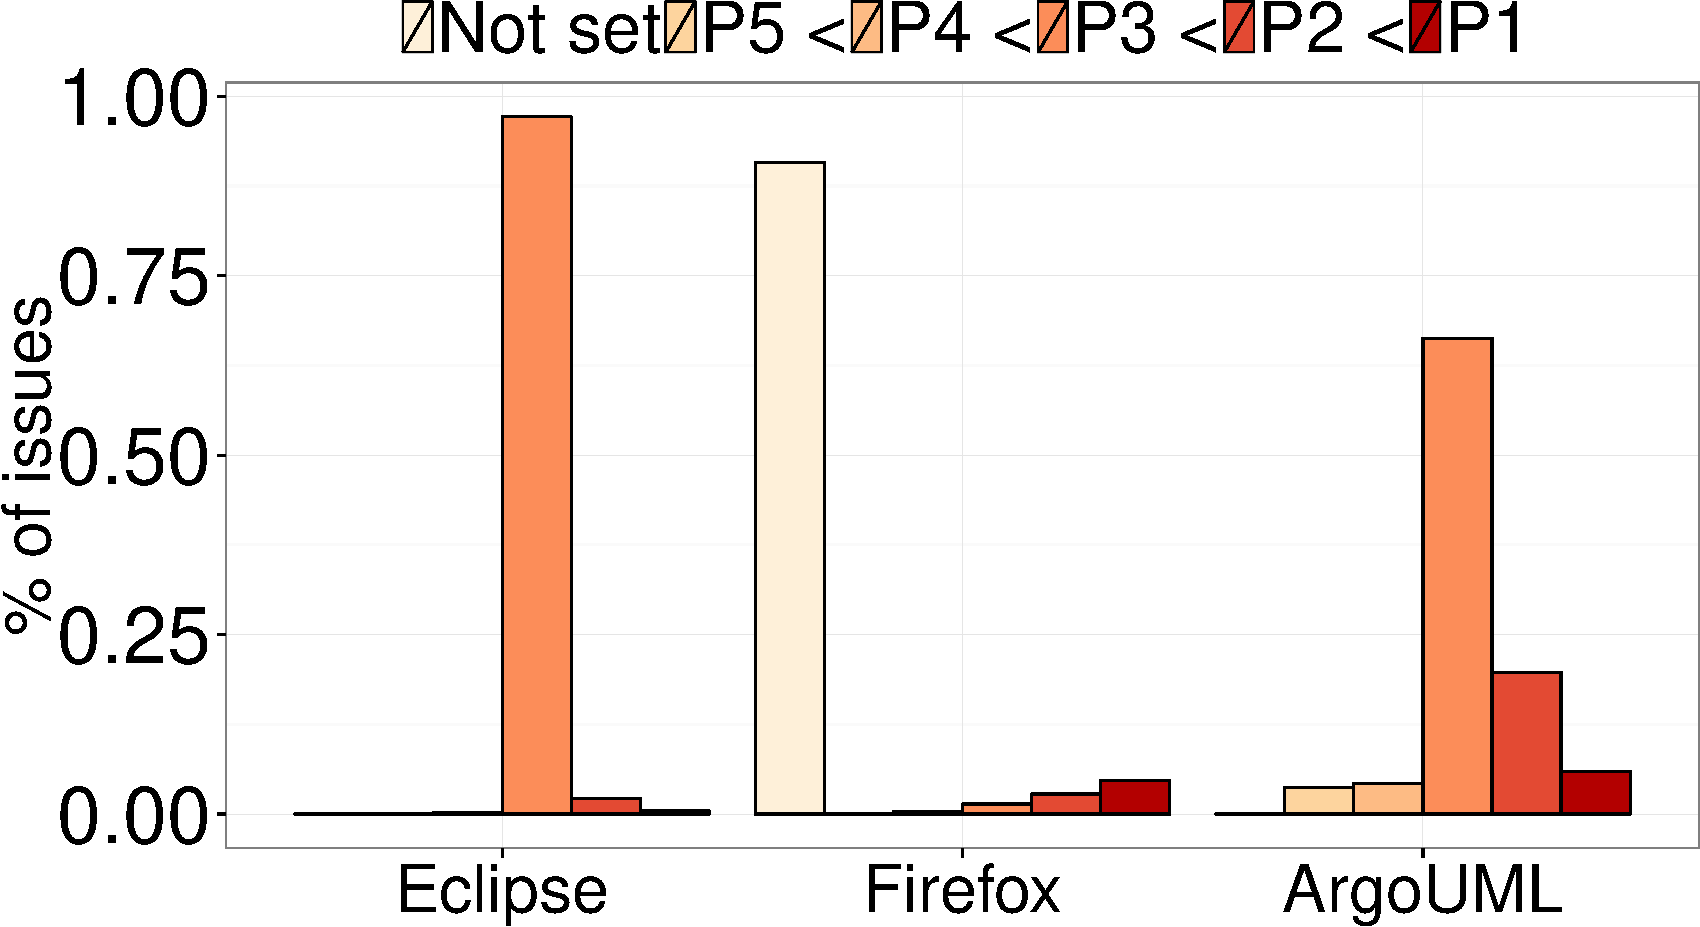
\includegraphics[width=0.60\textwidth,keepaspectratio]
		{chapters/chapter4/figures/issues_per_priority.pdf}
	}

	\subfloat[Severity values. The ArgoUML project does not use the severity field]{
		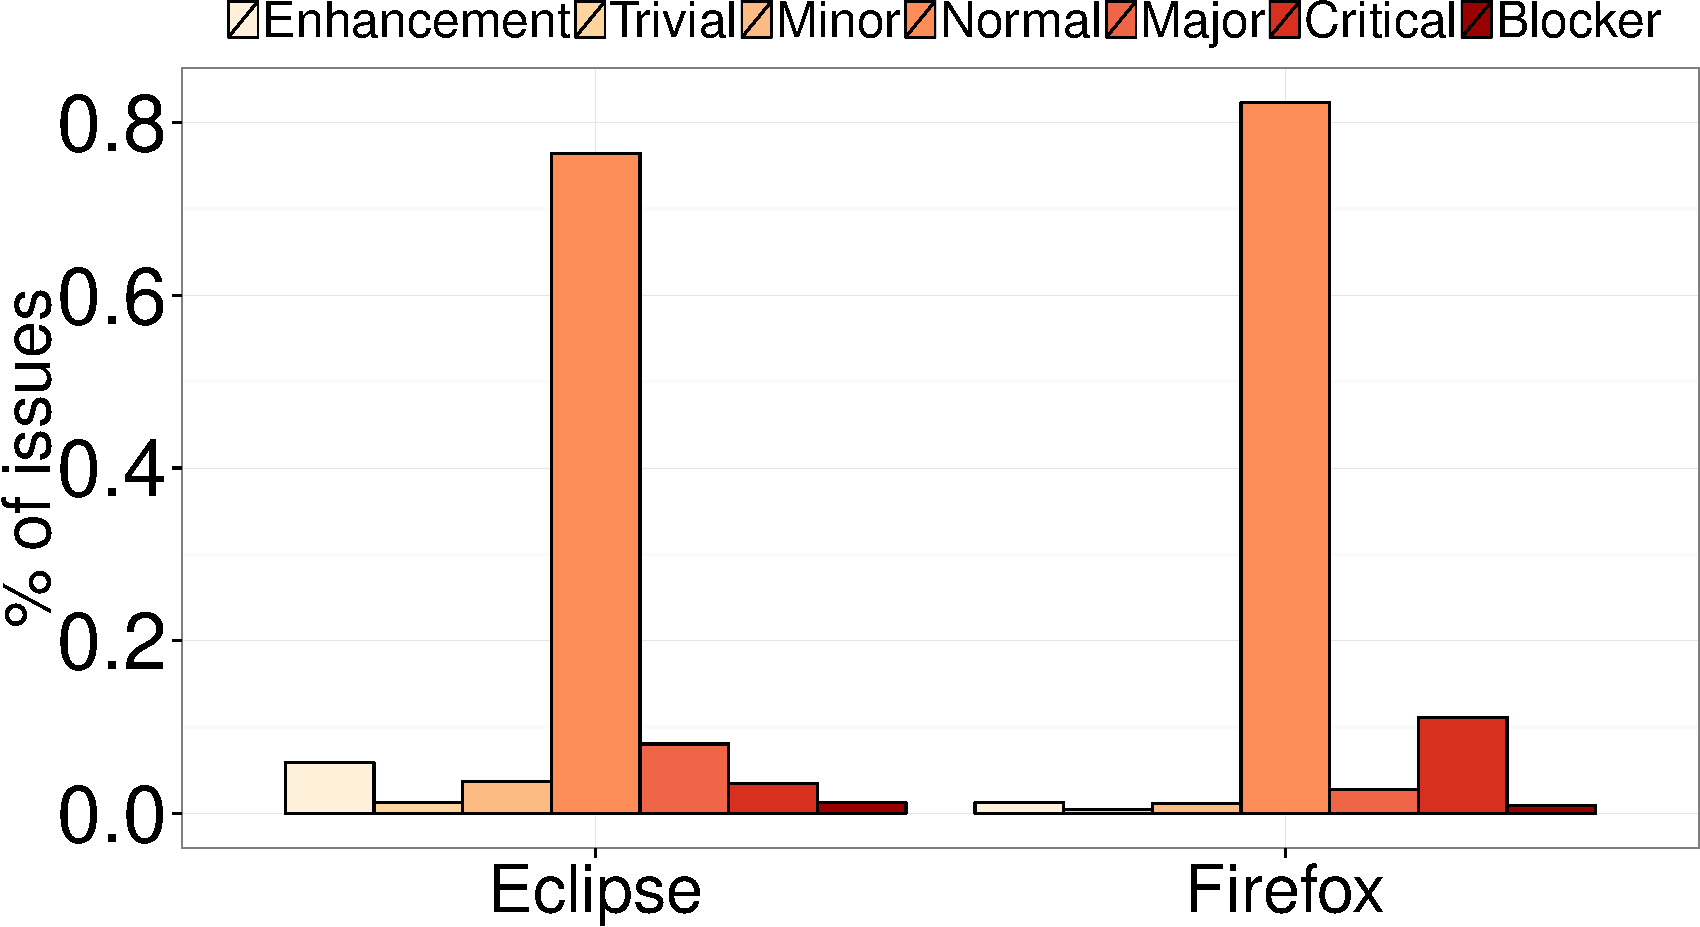
\includegraphics[width=0.60\textwidth,keepaspectratio]
		{chapters/chapter4/figures/issues_per_severity.pdf}
	}

	\subfloat[Fixed issues vs. Not fixed yet]{
		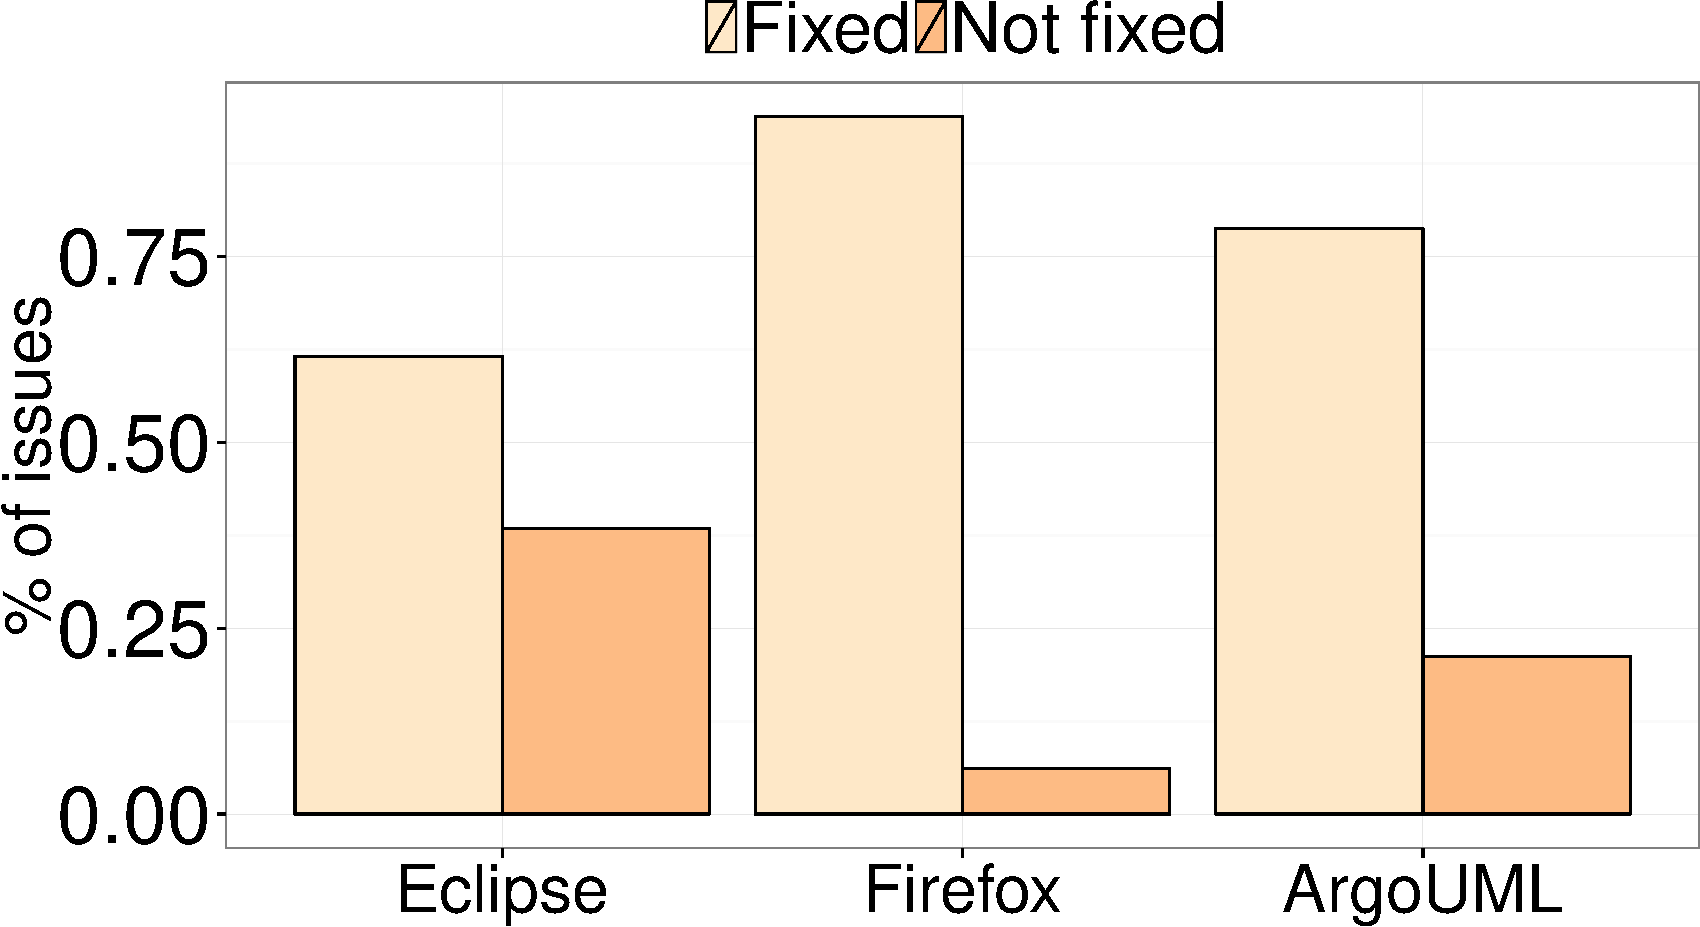
\includegraphics[width=0.60\textwidth,keepaspectratio]
		{chapters/chapter4/figures/neveresolved_resolved.pdf}
	}
	\caption{\textbf{Exploratory analysis of the studied projects.} We
		present the ratio of addressed issues per priority, severity, and the
		ratio of addressed vs. not addressed yet issues (\eg \textit{WONTFIX} or
	\textit{WORKSFORME})}
	\label{ch4:fig:preliminary_studied_system}
\end{figure}

\hyperref[ch4:fig:preliminary_studied_system]{Figure}~\ref{ch4:fig:preliminary_studied_system}
shows an exploratory analysis of our studied projects. We plot the proportion of
issues per priority and severity level, as well as the proportion of issues that
were addressed and not addressed (\eg resolution is \textit{WONTFIX} or
\textit{WORKSFORME}). We observe that for the majority of the issues, the
priority and severity levels remain at the default value. For example, the vast
majority of the priority values are set to P3 (in the Eclipse and ArgoUML
projects) or ``- -'' (in the Firefox project). We also observe that Firefox is
the project with the highest proportion of addressed issues.

\hyperref[ch4:tbl:consideredReleases]{Table}~\ref{ch4:tbl:consideredReleases} shows the
studied period and range of releases, as well as the number of releases and
issue reports. We focus our study on the releases for which we could recover a
list of issue IDs from the release notes. We collected a total of 20,995 issue
reports from the three studied projects. Each issue report corresponds to an
issue that was addressed and could be mapped directly to a release. We present
an overview of the release engineering processes of each studied project below.

\subsubsection*{\textbf{\textit{Eclipse Release Engineering}}}\label{eclipse:releng}

The release engineering of the Eclipse project is composed by {\em
nightly/integration} builds that are followed by {\em milestones} builds and
{\em release candidate} builds. Nightly or integration builds are the least
stable builds and are tested by the early adopters that are following the
eclipse developer mailing lists. For instance, integration builds are not
supposed to be announced through links, blogs, or wikis that are related to the
respective Eclipse
project.\smartfoot{\url{https://eclipse.org/projects/dev_process/development_process.php\#6_Development_Process}} 

{\em Milestone} and {\em release candidate} builds are more stable and can be
announced by external links such as blogs and wikis. The goal is to reach
external early-adopters from outside the developer mailing lists. However, the
external links that refer to such builds should warn that they are not as stable
as official releases. The main difference between a release candidate build and
a milestone build is that a release candidate goes through a rigorous {\em
testing pass}
process.\smartfoot{\url{https://www.eclipse.org/eclipse/development/plans/freeze_plan_4_4.php}}

The testing pass process consists of intensive testing activities that are
performed by the development team and community to find regression and {\em
stop-ship} bugs. In case stop-ship bugs are found late in the process, the
release schedule may be slipped to accommodate the fixes for such
bugs.\footnotemark[15]

After the testing pass stage, a {\em fixing pass} stage starts. The fixing pass stage
consists on prioritizing and fixing the most severe bugs that are found at the
testing pass stage. By the end of a fixing pass stage, another release candidate is
produced. The process of performing testing passes and fixing passes is done through
several iterations (\ie many release candidates are produced). 

The last release candidate is submitted to a {\em code freeze} stage. The {\em
code freeze} is a period at which the rules to integrate changes in the software
project becomes more strict. For instance, new changes may be integrated only if
they are solving special requirements such as translations or documentation
fixing.\footnotemark[15] Such a period is important because it helps the
development team to stabilize the project just before creating an official
release.

Official releases are categorized as {\em major}, {\em minor}, and {\em service} 
releases.\smartfoot{\url{https://www.eclipse.org/projects/handbook/\#release}}
Major releases include API changes. Minor releases add new functionalities but
are compatible with the API of prior versions. Finally, service releases include
bug fixes only (\ie without significant addition of new functionality). Both
major and minor releases have to pass through a {\em release review} process. A
release review aims at getting feedback about the release cycle that was
performed. The main goal is to find areas of improvement and if the development
process is being open and
transparent.\smartfoot{\url{https://www.eclipse.org/projects/handbook/\#release-review}}

\subsubsection*{\textbf{\textit{Firefox Release Engineering}}}\label{firefox:releng}

The release engineering process of the Firefox project uses a {\em rapid} (or
{\em a short}) release cycle, \ie a release cycle of 6 weeks duration. In
addition, the process also include {\em pipelining} releases (also known as {\em
release training}) as a means to stabilize the official release, so that they
can be shipped to end users.

The pipelining process develops releases through several channels.
As the release progresses through these channels, the stability of the release
increases and less severe bugs are more likely to be uncovered. The Firefox project team
uses four channels to develop releases: {\em NIGHTLY}, {\em AURORA}, {\em BETA},
and {\em RELEASE}
channels.\smartfoot{\url{http://mozilla.github.io/process-releases/draft/development_overview/}}

The NIGHTLY channel produces a release every night (\ie as soon as features are
ready). This nightly release is built from the {\em mozilla-central} repository and has
the lowest stability of the
channels.\smartfoot{\url{https://hg.mozilla.org/mozilla-central/}}
The AURORA channel produces a release every six weeks. However, some new
features may be disabled if they are not stable enough. At the end of the cycle
of the AURORA channel (the sixth week), the release management team decides which
of the issues that were further stabilized are good enough to migrate to the BETA
channel. Again, the goal of the BETA channel is to stabilize the new features
and disable the features that are not stable enough by the end of the cycle.
Finally, the features that are stable enough to survive at the BETA channel are
moved further to the RELEASE channel, from which an official major release is
produced.\footnotemark[18]

In the Firefox release engineering process, the release schedule is not slipped
to accommodate issues that are not stable enough by the end of the release
cycle. Instead, the development team holds such issues back to be shipped in
future releases when a greater degree of stability is achieved.\footnotemark[18]
Also, an issue may be integrated directly into the AURORA or BETA channels (\ie
the issue is {\em uplifted}), but such cases are exceptions (\eg very critical
security issues that must be released as soon as possible).\footnotemark[18] 

The Firefox project also ships {\em Extended Support Releases} (ESR) that are
based on prior official Firefox releases. ESRs are meant to institutions such as
business organizations, schools, and universities that need to manage their
Firefox desktop client. ESRs provide one year of support for security and bug
fixes of prior Firefox official releases. ESRs are important for organizations
that are not able to follow the fast pace that the Firefox major release
evolves.\smartfoot{\url{https://www.mozilla.org/en-US/firefox/organizations/faq/}}

\subsubsection*{\textbf{\textit{ArgoUML Release Engineering}}}\label{argouml:releng}

In the ArgoUML release engineering process, there are five types of releases:
{\em development}, {\em alpha}, {\em beta}, {\em stable}, and {\em stable patch}
releases. {\em Development} releases are the least stable, while {\em stable}
releases are the official releases that are intended to be widely adopted by the
users.\smartfoot{\url{http://argouml.tigris.org/wiki/How_to_Create_a_Stable_Release}}
 
{\em Development} releases are generated during the {\em development} stage.
The {\em development} stage may take from one to several months. During this
stage, the development team strives to produce a {\em development} release each
month. {\em Development releases} are not supposed to be used by end users. Such
releases are only advertised to users if there is a purpose of recruiting new
developers to implement and test new features.\footnotemark[21]

After the {\em development} stage, the {\em alpha} stage starts. The {\em
alpha} stage is also referred as the {\em enhancement freeze} point. All of the
enhancements that are not stable enough before the start of the {\em alpha}
stage are not included into the {\em stable} release. According to the ArgoUML
documentation, the {\em alpha} stage usually takes a ``{\em couple of weeks}''
and the development team strives to make a release each week.\footnotemark[21]

The {\em alpha} stage is followed by the {\em beta} stage. The {\em beta}
stage is also referred as the {\em bug-fix freeze} point, \ie all of the (less
severe) bug-fixes that could not be completed before the start of the {\em beta}
stage are omitted from the {\em stable release}. Such remaining bugs are listed
on the ``{\em known problems}'' document that is to be published along with the
{\em stable} release. {\em Beta} releases are more stable than {\em alpha} releases
and are also referred as {\em release candidates}. For instance, {\em beta}
releases should not contain high priority bugs (\ie issues for which the
priority is either P1 or P2).  The {\em beta} stage is supposed to last for a
couple of weeks with a {\em beta} release being generated each week. Finally,
the {\em beta} stage is marked by intense testing activities after each release
candidate. When the team is confident that the {\em beta} release is stable
enough, the official {\em stable} release is generated with no code changes from
the last {\em beta} release.\footnotemark[21]

The last type of ArgoUML release is the {\em stable patch} release. {\em Stable
patch} releases are generated if critical bugs are found after the publication
of the {\em stable} release. The {\em stable patch} release contains the fixes
for the eventual critical bugs that are found upon {\em stable}
releases.\footnotemark[21] The ArgoUML team strives to ship a {\em stable}
release every 8
months.\smartfoot{\url{http://argouml.tigris.org/wiki/Strategic_Planning}}

\subsection{Data Collection}

\hyperref[ch4:fig:overview]{Figure}~\ref{ch4:fig:overview} provides an overview of our
data collection approach---how we collect and organize the data in order to
perform our empirical study. We create a relational database that describes the
delivery of addressed issues in the studied projects. We briefly describe our
data sources, and each step that are involved in the database construction process. 

\subsubsection*{\textbf{\textit{Step 1: Fetch delivered issue IDs}}}


\begin{table}
	\footnotesize
	\caption{\textbf{Overview of the studied projects.} We present the number
	of studied releases, issues, the studied period and the median time
	between releases.}
	\label{ch4:tbl:consideredReleases}
	%\resizebox{\columnwidth}{!}{
	%\begin{tabular}{L{1.45cm}C{2.5cm}C{1.5cm}C{0.7cm}R{0.75cm}R{2.25cm}}
	\begin{tabular}{L{1.65cm}C{2.5cm}C{1.5cm}C{1.0cm}R{2.45cm}R{4.25cm}}
		\hline 
		\centering{\textbf{Project}} & \textbf{Studied period} &
		\textbf{Releases} & \centering{\textbf{\# of \newline releases}}
		& 
		\centering{\textbf{\# fixed issues}} & \centering{\textbf{Median
time between releases (weeks)}}\tabularnewline
		\hline 
		\hline 
		\textbf{Eclipse (JDT)} & 03/11/2003 - 12/02/2007 & 2.1.1
		- 3.2.2 & 11 & 3344 & 16\tabularnewline
		\hline 
		\textbf{Firefox} & 05/06/2012 - 04/02/2014 & 13 - 27 &
		15 & 3121 & 6\tabularnewline
		\hline 
		\textbf{ArgoUML} & 18/08/2003 - 15/12/2011 & 0.14 - 0.34
		& 17 & 14530 & 26 \tabularnewline
		\hline 
	\end{tabular}
\end{table}

\begin{figure}
	\centering
	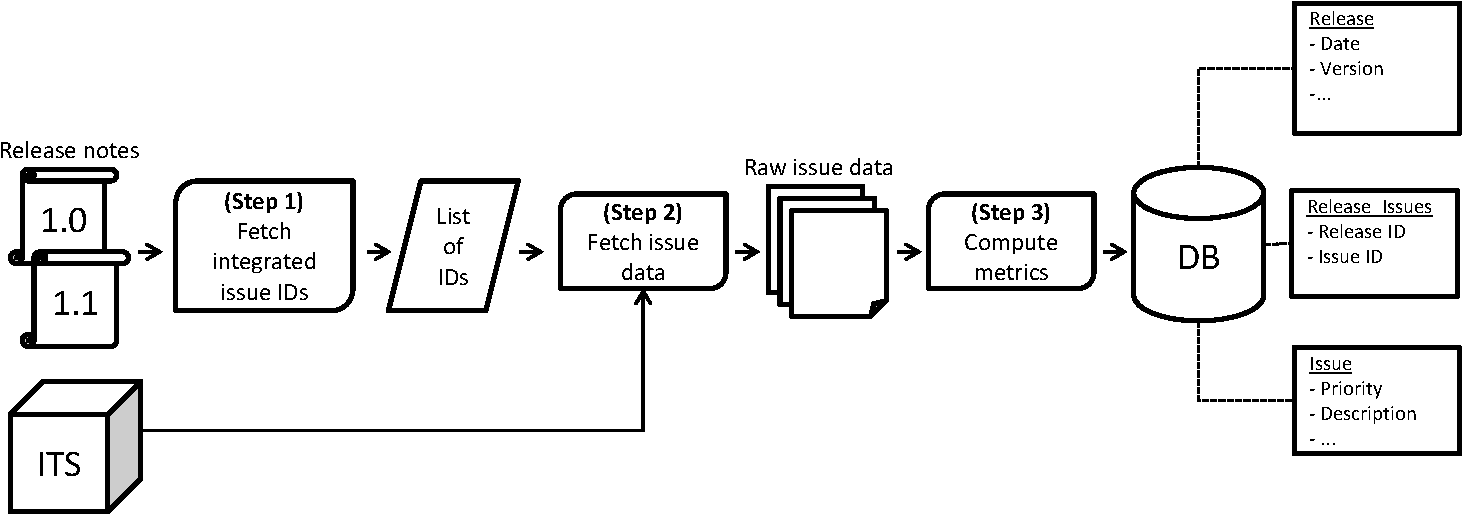
\includegraphics[width=\textwidth]{chapters/chapter4/figures/database_construction.pdf}
	\caption{\textbf{Data collection.} An overview of our approach to
	collect the needed data for studying delivery delay.}
	\label{ch4:fig:overview}
\end{figure} 

In Step 1, we consult the release notes of each studied project to identify the
release into which an addressed issue was delivered. A release note is a
document that describes the content of a release. For instance, a release note
might provide information about the improvements that are included in a release (with
respect to prior releases), the new features, the fixed issues, and the known
problems. The Eclipse, ArgoUML, and Firefox projects publish their release notes on their
respective websites.\smartfoot{\url{https://www.mozilla.org/en-US/firefox/releases/}}

Unfortunately, release notes may not mention all of the fixed issues that have
been delivered through a release. This limitation hinders the possibility of
studying issues that were fixed but have not been delivered, since we cannot
claim that an issue that is not listed in a release note was not delivered (\eg
the development team may forget to list some delivered fixed issues). However,
the fixed issues that are listed in a release note are more likely to have been
shipped to the end users (\ie it is unlikely that a release note would mention a fixed
issue that was not delivered). Hence, we choose to use release notes as a means
of linking fixed issues to releases in our database, despite the incompleteness
of such release notes---the release where we claim that an issue has been
delivered is more likely to be correct (we elaborate more on this point in
\hyperref[ch4:threats]{Section}~\ref{ch4:threats}).

The output of Step 1 is a list of the issue IDs that have been fixed and
delivered. To retrieve such a list for the Eclipse and Firefox projects, we
wrote a script to extract the listed issue IDs from all the release notes and
insert them into our database. The retrieved issue IDs are used to fetch the
issue report meta-data from the corresponding ITSs. In our database, we also
store the dates and version number of each release. 

\subsubsection*{\textbf{\textit{Step 2: Fetch issue data}}}

We use the collected issue IDs from Step~1 to retrieve information from their corresponding
issue reports, which
are recorded in the ITSs. Not all release notes of
the ArgoUML project
list the fixed issues of an official release. When they do,
only a few issues are listed (\eg
1-4).\smartfoot{\url{http://argouml.tigris.org/wiki/ReleaseSchedule/Past_Releases_in_Detail}}
To increase our sample of fixed issues for the ArgoUML project, we rely on its
ITS. We use the milestone field of
the issue reports to approximate the release into which an issue was delivered.
Development milestones are counted towards the next official releases. For
instance, the development milestone
0.33.7\smartfoot{\url{http://argouml.tigris.org/issues/show_bug.cgi?id=4914}}
is counted towards the official release 0.34. The output of Step 2 is the raw
issue report data that is collected from ITSs.

Finally, to determine when an issue was fixed, we use the latest change to the
RESOLVED-FIXED status of that issue.  For instance, if an issue has its status
changed from RESOLVED-FIXED to REOPENED at $t_1$ and the status changes back to
RESOLVED-FIXED at $t_2$ (without changing again), we consider the corresponding
date of $t_2$ as the fix date. Also, we use the RESOLVED-FIXED status rather
than the VERIFIED-FIXED status, since we found that all of the issues that are
mapped to releases went through the RESOLVED-FIXED state before being delivered, while
only a small percentage went through the VERIFIED-FIXED state. For example, only 17\% of
fixed issues in the Firefox project went through the VERIFIED-FIXED state.
We focus on issues that were resolved as RESOLVED-FIXED because they involve
changes to the source and/or test code that must be integrated into a release
before becoming visible to end users.

\subsubsection*{\textbf{\textit{Step 3: Compute metrics}}} \label{settings:step3}

After collecting the release date for each addressed issue, we compute all of the
attributes that may share a relationship with the types of delivery delay that
are presented in
\hyperref[ch2:deliverydelay]{Section}~\ref{ch2:deliverydelay}.

We first compute the delivery delay of addressed issues in terms of number of
releases (see~\hyperref[def:1]{Definition}~\ref{def:1}). We group this type of
delivery delay into four buckets: \textit{next}, \textit{after-1},
\textit{after-2}, and \textit{after-3-or-more}. The \textit{next} bucket
contains addressed issues that are delivered immediately. The \textit{after-1},
\textit{after-2}, and \textit{after-3-or-more} buckets contain addressed issues
for which delivery is skipped by one, two, or three or more releases,
respectively.
\hyperref[ch4:fig:fixToIntegration]{Figure}~\ref{ch4:fig:fixToIntegration} shows
the distribution of the addressed issues among buckets for each studied project.
The ArgoUML project has the highest percentage of addressed issues that fall
into the \textit{next} bucket (66\%), whereas \textit{next} accounts for only
2\% and 38\% of addressed issues in the Firefox and Eclipse projects,
respectively. 

\begin{figure}
	\centering
	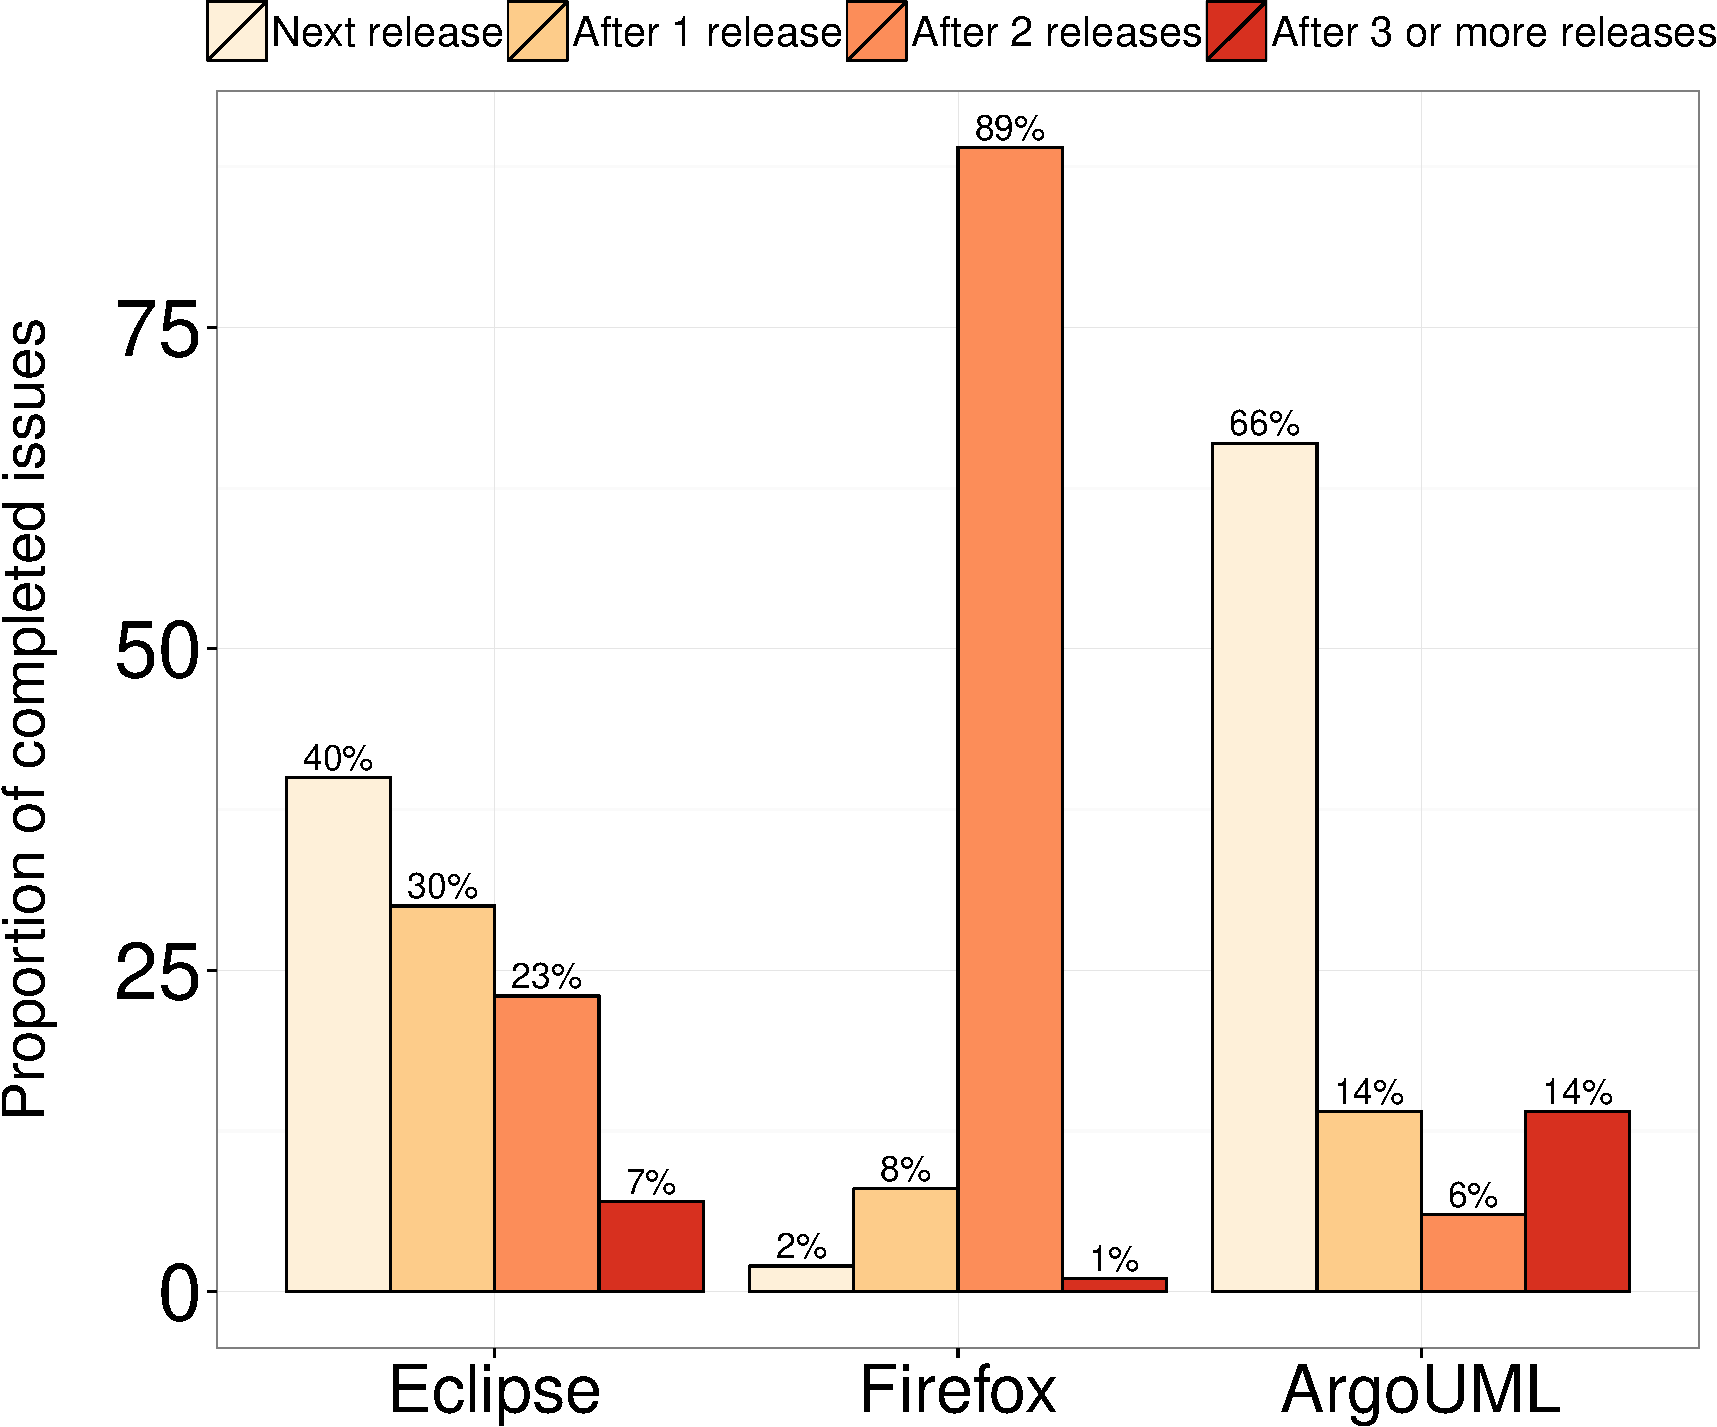
\includegraphics[width=0.7\textwidth]
	{chapters/chapter4/figures/CS_rq1-datasets.pdf}
	\caption{\textbf{Distribution of addressed issues per bucket.} The issues are
		grouped into \textit{next}, \textit{after-1}, \textit{after-2}, and
	\textit{after-3-or-more} buckets.}
	\label{ch4:fig:fixToIntegration}
\end{figure}

\begin{figure}
	\centering
	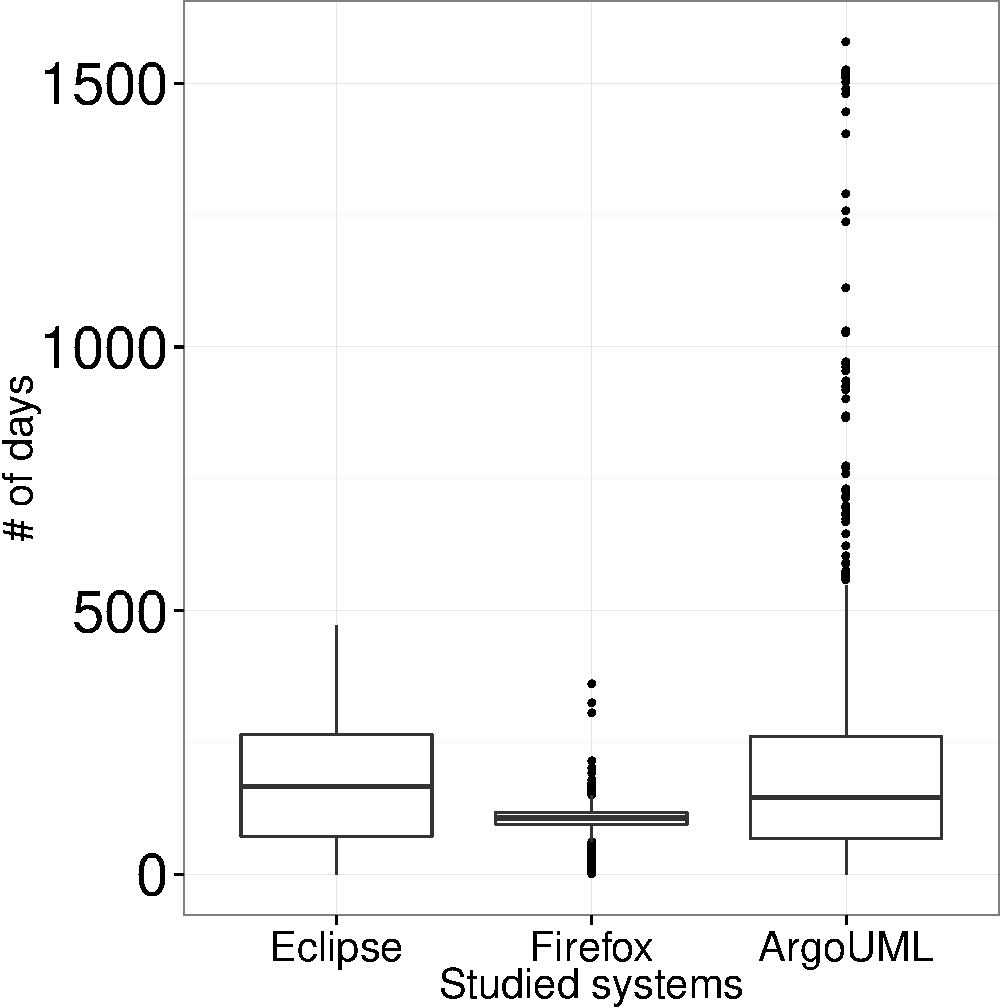
\includegraphics[width=0.60\textwidth,keepaspectratio]
	{chapters/chapter4/figures/boxplot-days-per-system.pdf}
	\caption{\textbf{Delivery delay in terms of days.} The medians 
		are 166, 107, and 146 days for the Eclipse, Firefox, and
		ArgoUML projects, respectively.
	}
	\label{ch4:fig:beanplot_days}
\end{figure}

Next, we compute the delivery delay in terms of number of days (see
\hyperref[def:2]{Definition}~\ref{def:2}).
\hyperref[ch4:fig:beanplot_days]{Figure}~\ref{ch4:fig:beanplot_days} shows the
distribution of delivery delay in terms of days for each studied project. The
Firefox project has the least skewed distribution of delivery delay. We use both
\hyperref[def:1]{Definitions}~\ref{def:1} and~\ref{def:2} of delivery delay to
address \hyperref[ch4:rq1]{RQ1}-\hyperref[ch4:rq4]{RQ4}.   

Finally, we identify issues that have a prolonged delivery delay in each studied
project (see \hyperref[def:3]{Definition}~\ref{def:3}). We group addressed
issues into \textit{prolonged delay} and \textit{normal delay} buckets.
Addressed issues, of which delivery delay is at least one MAD above the median
delivery delay of a subject project, fall into the \textit{prolonged delay}
bucket.  \hyperref[ch4:fig:beanplot_days]{Figure}~\ref{ch4:fig:beanplot_days}
shows that a prolonged delivery delay in one project may be a normal delivery
delay in another project (\eg the ArgoUML project {\em vs.} the Firefox
project). This figure highlights the importance of performing this analysis for
each project individually. We use this data to address \hyperref[ch4:rq5]{RQ5}
and \hyperref[ch4:rq6]{RQ6}.

We use exploratory models to study the relationship between attributes of
addressed issues (\eg severity and priority) and delivery delay. Our goal is to
understand which attributes are important for modeling the delivery delay of
addressed issues. \\

\section{Results} \label{ch3:results}

In this section, we present the motivation, approach, and results for each
investigated RQ. 

\subsection{RQ1: How often are addressed issues prevented
from being released?}\label{ch4:rq1}

\subsubsection*{RQ1: Motivation}

Users and contributors care most about the time for an addressed issue to become
available rather than the time duration to fix it. In this regard, it is
important to investigate whether addressed issues are being delivered
immediately (\eg in the next possible release) or not, since a large delivery
delay may frustrate users. In \hyperref[ch:rq1]{RQ1}, we investigate how often
addressed issues are being prevented from delivery. The analysis of
\hyperref[ch:rq1]{RQ1} is our first step toward understanding how long is the
delivery delay of addressed issues.

\subsubsection*{RQ1: Approach} 

We compute the delivery delay of addressed issues in terms of number of releases
and number of days (as shown in \hyperref[def:1]{Definitions}~\ref{def:1}
and~\ref{def:2}). Next, we analyze if addressed issues are being prevented from
being released solely because their fix occurs in the end of their release
cycle. For instance, Rahman and Rigby~\cite{rahman2015release} observe a
rush-to-release in which many issues are addressed near the release date. For
each addressed issue, we compute the {\em fix timing} metric, which is the ratio
between (i) the remaining number of days---after an issue is addressed---for an
upcoming release over (ii) the duration in terms of days of its respective
release cycle (see
\hyperref[ch4:eq:fixtiming]{Equation}~\ref{ch4:eq:fixtiming}). The {\em fix
timing} values range from 0 to 1. A {\em fix timing} value close to 1 indicates
that an issue is addressed early in the release cycle, since the numerator and
denominator of \hyperref[ch4:eq:fixtiming]{Equation}~\ref{ch4:eq:fixtiming}
would be close to each other.

\begin{equation}
	\frac{\text{\# days that is remaining for a release}}{\text{release cycle duration}}
	\label{ch4:eq:fixtiming}
\end{equation}

\subsubsection*{RQ1: Results} \label{results:rq1}

\begin{figure}[!t]
	\centering
	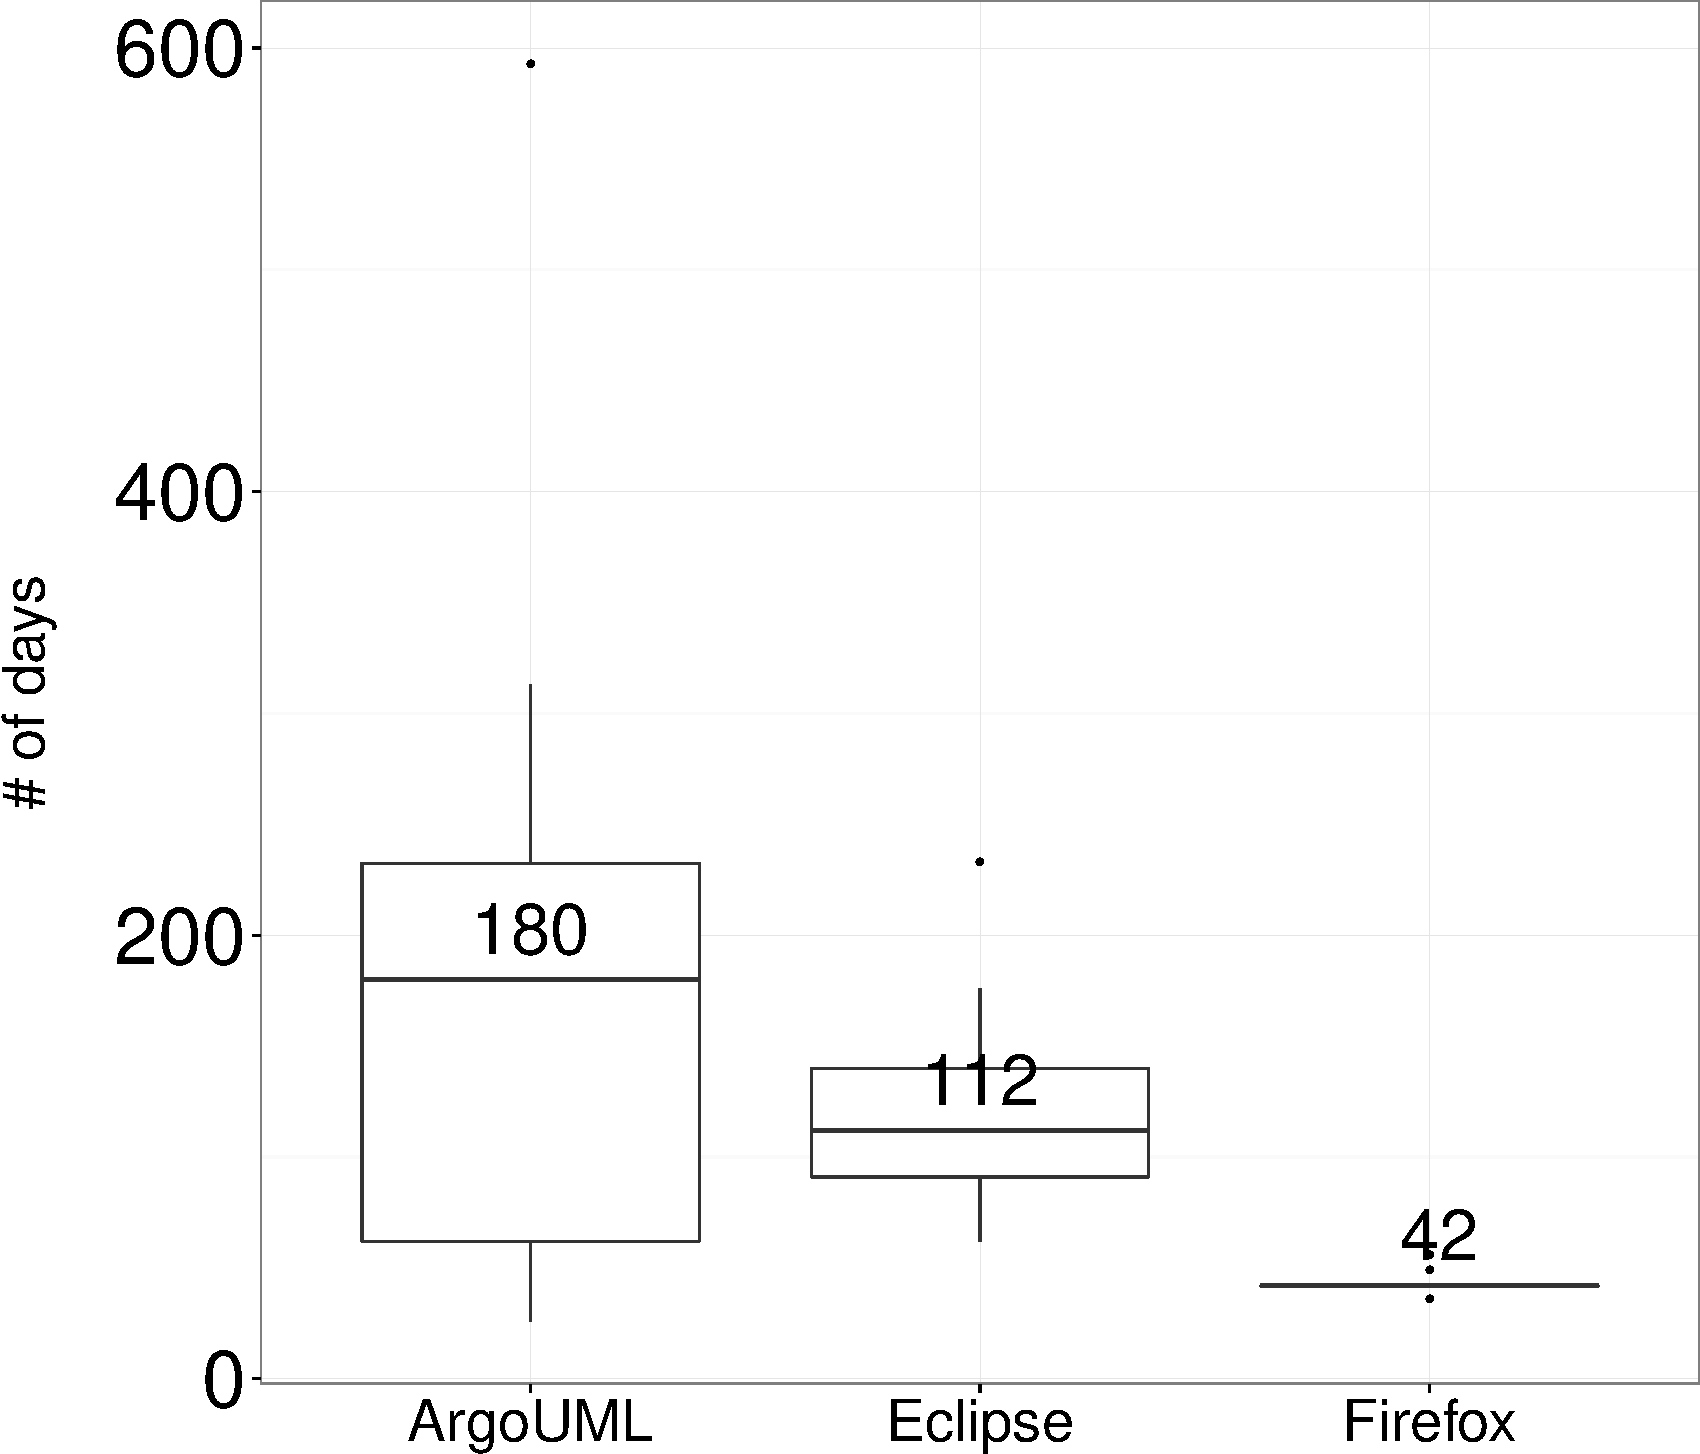
\includegraphics[width=0.7\textwidth]
	{chapters/chapter4/figures/RQ1_time_between_releases.pdf}
	\caption{\textbf{Number of days between the studied releases of the
	ArgoUML, Eclipse, and Firefox projects.} The number shown over each
boxplot is the median interval.}  
	\label{ch4:fig:releaseIntervals}
\end{figure}

\noindent\finding{Addressed issues usually
miss the next release in the Firefox project.}{find1}
\hyperref[ch4:fig:releaseIntervals]{Figure}~\ref{ch4:fig:releaseIntervals} shows the
difference between the studied projects in terms of the time interval between
their releases. The median time in days for the Firefox project (42 days) is
approximately $\frac{1}{4}$ that of the ArgoUML project (180 days), and
$\frac{1}{3}$ that of the Eclipse project (112 days). Unlike the Eclipse and
Firefox projects, the distribution for the ArgoUML project is skewed. In
addition, \hyperref[ch4:fig:fixToIntegration]{Figure}~\ref{ch4:fig:fixToIntegration}
shows that the vast majority of addressed issues for the Firefox project is
delivered
\textit{after-2} releases, whereas for the Eclipse and ArgoUML projects, the
majority is delivered in the \textit{next} release. 

The reason for the difference may be due to the release policies that are
followed in each project. For example,
\hyperref[ch4:fig:releaseIntervals]{Figure}~\ref{ch4:fig:releaseIntervals} shows that
the Firefox project releases consistently every 42 days (six weeks), whereas the
time intervals between the releases of the ArgoUML project vary from 50 to 220
days. Indeed, the release guidelines for the ArgoUML project state that the
ArgoUML team should release at least one stable release every 8 months (see
\hyperref[argouml:releng]{Section}~\ref{argouml:releng}). The delivery
consistency of the Firefox releases might lead to addressed issues being prevented
from a greater number of releases, since the Firefox project rigidly adhere to a
six-week release schedule despite accumulating issues that could not be
delivered (see \hyperref[firefox:releng]{Section}~\ref{firefox:releng}). 

Although an addressed issue usually misses the next release in the Firefox
project, issues are usually shipped faster when compared to the other projects.
Indeed, \hyperref[ch4:fig:beanplot_days]{Figure}~\ref{ch4:fig:beanplot_days} shows that
addressed issues in the Firefox project take a median of 107 days to be
released, while it takes 166 and 146 days in the Eclipse and ArgoUML projects,
respectively.\\

\noindent\finding{34\% to 60\% of addressed issues had their delivery
prevented from at least one release in the traditionally released
projects.}{find2}
\hyperref[ch4:fig:fixToIntegration]{Figure}~\ref{ch4:fig:fixToIntegration} shows
that 98\% of the addressed issues in the Firefox project are prevented from
delivery in at least one release. However, for the projects that adopt a more
traditional release cycle, \ie the ArgoUML and Eclipse projects, 34\% to 60\%
of the addressed issues are prevented from delivery in at least one release.
This result indicates that even though an issue is addressed, its delivery may be
prevented by one or more releases, which can frustrate end users.\\

\begin{figure}[!t]
	\centering
	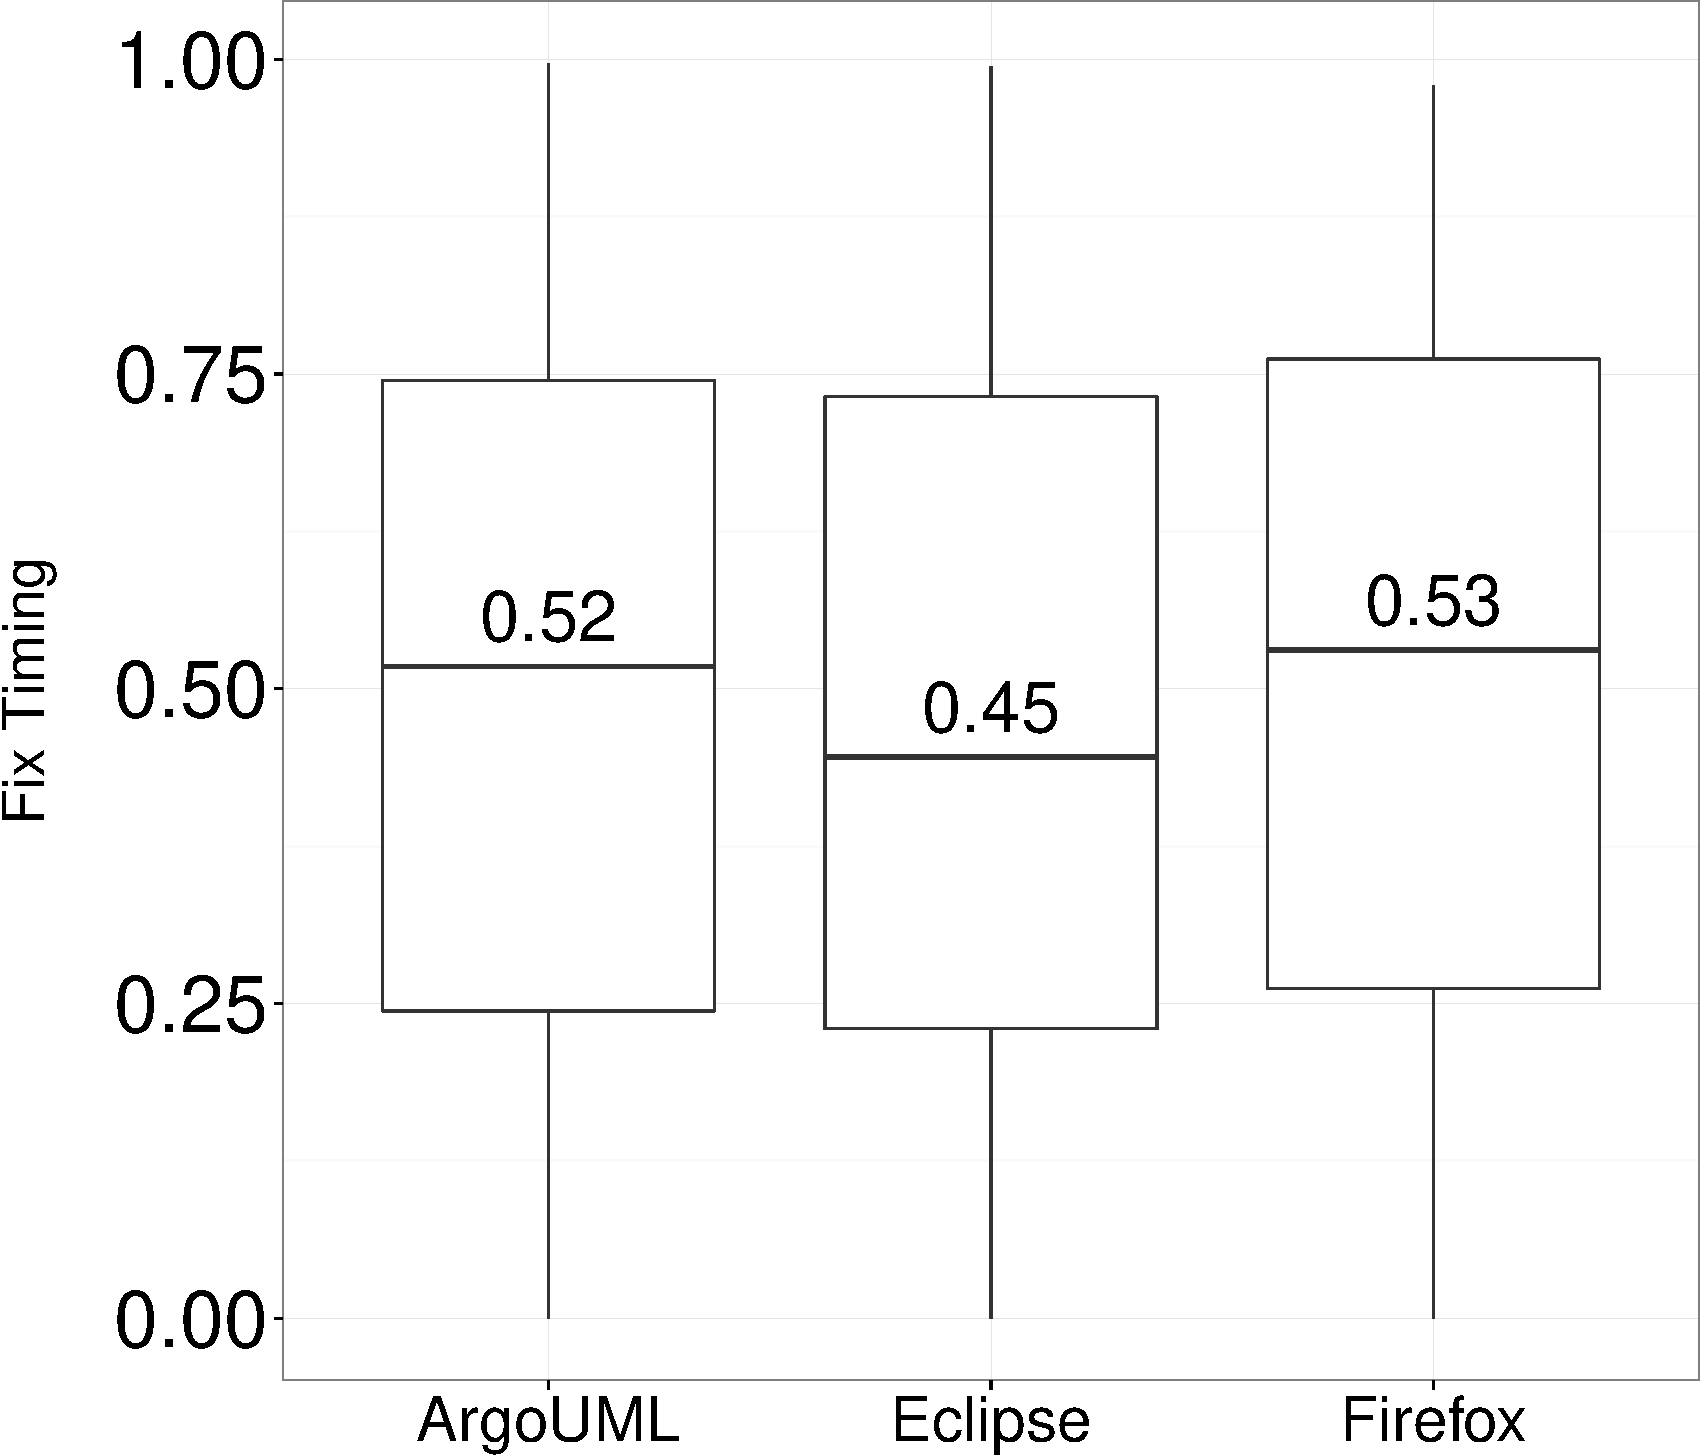
\includegraphics[width=0.7\textwidth]
	{chapters/chapter4/figures/addressing_stage.pdf}
	\caption{\textbf{Fix timing metric.} We present the
		distribution of the \textit{fix timing} metric for addressed
		issues that are prevented from delivery in at least one release.}
	\label{ch4:fig:boxplotTimeWindow}
\end{figure}

\noindent\finding{Many issues that were prevented from delivery are
addressed well before the upcoming release date.}{find3} Addressed issues could be prevented
from delivery because they were addressed late in the release cycle, \eg one day
or one week before the upcoming release date. To check whether addressed issues are
being prevented from delivery mostly because they are being addressed late in the
release cycle, we compute the \textit{fix timing} metric. 

\hyperref[ch4:fig:boxplotTimeWindow]{Figure}~\ref{ch4:fig:boxplotTimeWindow} shows the
distribution of the \textit{fix timing} metric for each project. The smallest
\textit{fix timing} median is observed for the Eclipse project, which is 0.45.
For the ArgoUML and Firefox projects, the median is 0.52 and 0.53, respectively.
The \textit{fix timing} medians are roughly in the middle of the release.
Moreover, the boxes extend to cover between 0.25 and 0.75. The result suggests
that, in the studied projects, issues that are prevented from delivery are
usually addressed $\frac{1}{4}$ to $\frac{3}{4}$ of the way through a release.
Hence, it is unlikely that most addressed issues are prevented from delivery
solely because they were addressed too close to an upcoming release date.

\conclusionbox{The delivery of 34\% to 60\% of the addressed issues in the
	traditionally released projects and 98\% in the rapidly released project
	were prevented from delivery in at least one release. Furthermore, we
	find that many issues which delivery was prevented, were addressed well
before the releases from which they were omitted.}


\subsection{RQ2: Does the stage of the release cycle impact
delivery delay?}\label{ch4:rq2}

\subsubsection*{RQ2: Motivation}

An issue that is {\em addressed} before the production of a {\em release candidate}
may receive more attention, which may lead to a shorter delivery delay.
Analysis of the impact of integration stage may help researchers and
practitioners to reflect on how to reduce delivery delay or to increase
awareness about it.

\subsubsection*{RQ2: Approach} 

For each studied project, we tag addressed issues according to the stage during
which they were addressed. For example, if an issue was addressed during the {\em beta}
stage of the Firefox project (\ie at the BETA channel), we tag such issue as
being ``{\em addressed during beta}''. We then compare the distributions of
delivery delay in terms of days (\hyperref[def:2]{Definition}~\ref{def:2})
among the different stages of a release cycle. For example, in the Firefox
project, we compare the distributions of delivery delay between the {\em
NIGHTLY}, {\em ALPHA}, and {\em BETA} stages, since the {\em RELEASE} stage
corresponds to the official release itself.

To check whether there is at least one statistically significant difference
among distributions of delivery delay, we use the Kruskal-Wallis
test~\cite{kruskal1952use}. This test checks if two or more samples are likely
to come from the same population ({\em null hypothesis}). However, when there are three or
more distributions, the Kruskal-Wallis test does not indicate which distribution
is statistically different with respect to the others. For specific comparisons
between distributions, we use the Dunn test~\cite{dunn1964multiple}. The Dunn
test shows which distribution is statistically different from the others. To
counteract the problem of multiple comparisons~\cite{dunn1961multiple}, we use
the Bonferroni correction to adjust our obtained $p$-$values$.

Finally, we use Cliff's delta to check the magnitude of the observed
differences~\cite{cliff1993dominance}. For example, two distributions may be
statistically different, but the magnitude of such a difference may be
negligible. The higher the value of the Cliff's delta, the greater the magnitude
of the difference between distributions. We use the thresholds provided by
Romano~\etal~\cite{romano_2006} to perform our comparisons: {\em delta} $<$
0.147 ({\em negligible}), {\em delta} $<$ 0.33 ({\em small}), {\em delta} $<$
0.474 ({\em medium}), and {\em delta} $>=$ 0.474 ({\em large}).

We also compute the {\em fix timing} metric (as in \hyperref[ch4:rq1]{RQ1}).
However, this time we check whether addressed issues are being prevented mostly
because they were performed near a code freeze date---rather than the upcoming
release date. \hyperref[ch4:eq:fixtiming2]{Equation}~\ref{ch4:eq:fixtiming2} shows how
we adapt \hyperref[ch4:eq:fixtiming]{Equation}~\ref{ch4:eq:fixtiming} to compute the
{\em fix timing} metric to account for the code freeze date. For the Eclipse
project, we consider the date of the last {\em release candidate} as the code
freeze stage, while we consider the date of a {\em beta stage} as the code
freeze stage in the ArgoUML project.

\begin{equation}
	\frac{\text{\# days that is remaining for a code freeze}}{\text{release
	cycle duration}}
	\label{ch4:eq:fixtiming2}
\end{equation}

\subsubsection*{RQ2: Results}

\noindent\finding{Issues that are addressed during more stable stages of a
release cycle have a shorter delivery delay.}{find4}
\hyperref[ch4:fig:cycle_phases]{Figure}~\ref{ch4:fig:cycle_phases} shows the
distributions of delivery delay (in terms of days) per each release cycle stage
of the studied projects. For the Eclipse project, the stages are divided into
{\em milestones}, {\em RCs} (Release Candidates), and {\em code freeze} (see the
\hyperref[eclipse:releng]{release engineering} process of Eclipse). Indeed,
issues that are addressed during RCs have a shorter delivery delay when compared
to issues that were addressed during milestone releases. For the difference
between {\em milestones} and {\em RCs}, we observe a $p=1.47 \times 10^{-52}$
and a {\em large} effect-size of $delta=0.63$. All of the $p$-$values$ and
$deltas$ of our statistical analysis are shown in
\hyperref[ch4:tbl:statisticalrq2]{Table}~\ref{ch4:tbl:statisticalrq2}. Even
though delivery delay seems to be larger during the {\em code freeze} stage, we
do not observe a significant $p$-$value$ when comparing the {\em code freeze}
stage with the {\em RC} stage. Additionally, although we obtain a $p=0.02$ when
comparing the {\em code freeze} stage with the {\em milestone} stage, we obtain
a {\em negligible} effect-size ($delta=0.09$), which indicates that the
difference of the values between distributions is not significant. In fact, only
ten issues were addressed during the {\em code freeze} stage in our data, which
impairs statistical observations of trends in such a stage.

For the Firefox project, we observe that delivery delay tends to be
shorter as fixes are performed along more stable stages. For example, by
comparing the delivery delay values between the {\em NIGHTLY} and {\em
AURORA} stages, we observe a $p=5.1 \times 10^{-49}$ and a {\em medium}
effect-size of $delta = 0.40$ (the other comparisons are shown in
\hyperref[ch4:tbl:statisticalrq2]{Table}~\ref{ch4:tbl:statisticalrq2}).

Finally, for the ArgoUML project, we also observe a trend of shorter
delivery delay as the fixes are performed during more stable stages of release
cycles. For instance, when we compare the delivery delay of addressed issues of the {\em alpha}
and {\em beta} stages, we obtain a $p$-$value$ of $3.98 \times 10^{-09}$ and a {\em
large} effect-size of $delta = 0.98$.\\

\begin{figure}
	\centering
	\subfloat[Eclipse]{
		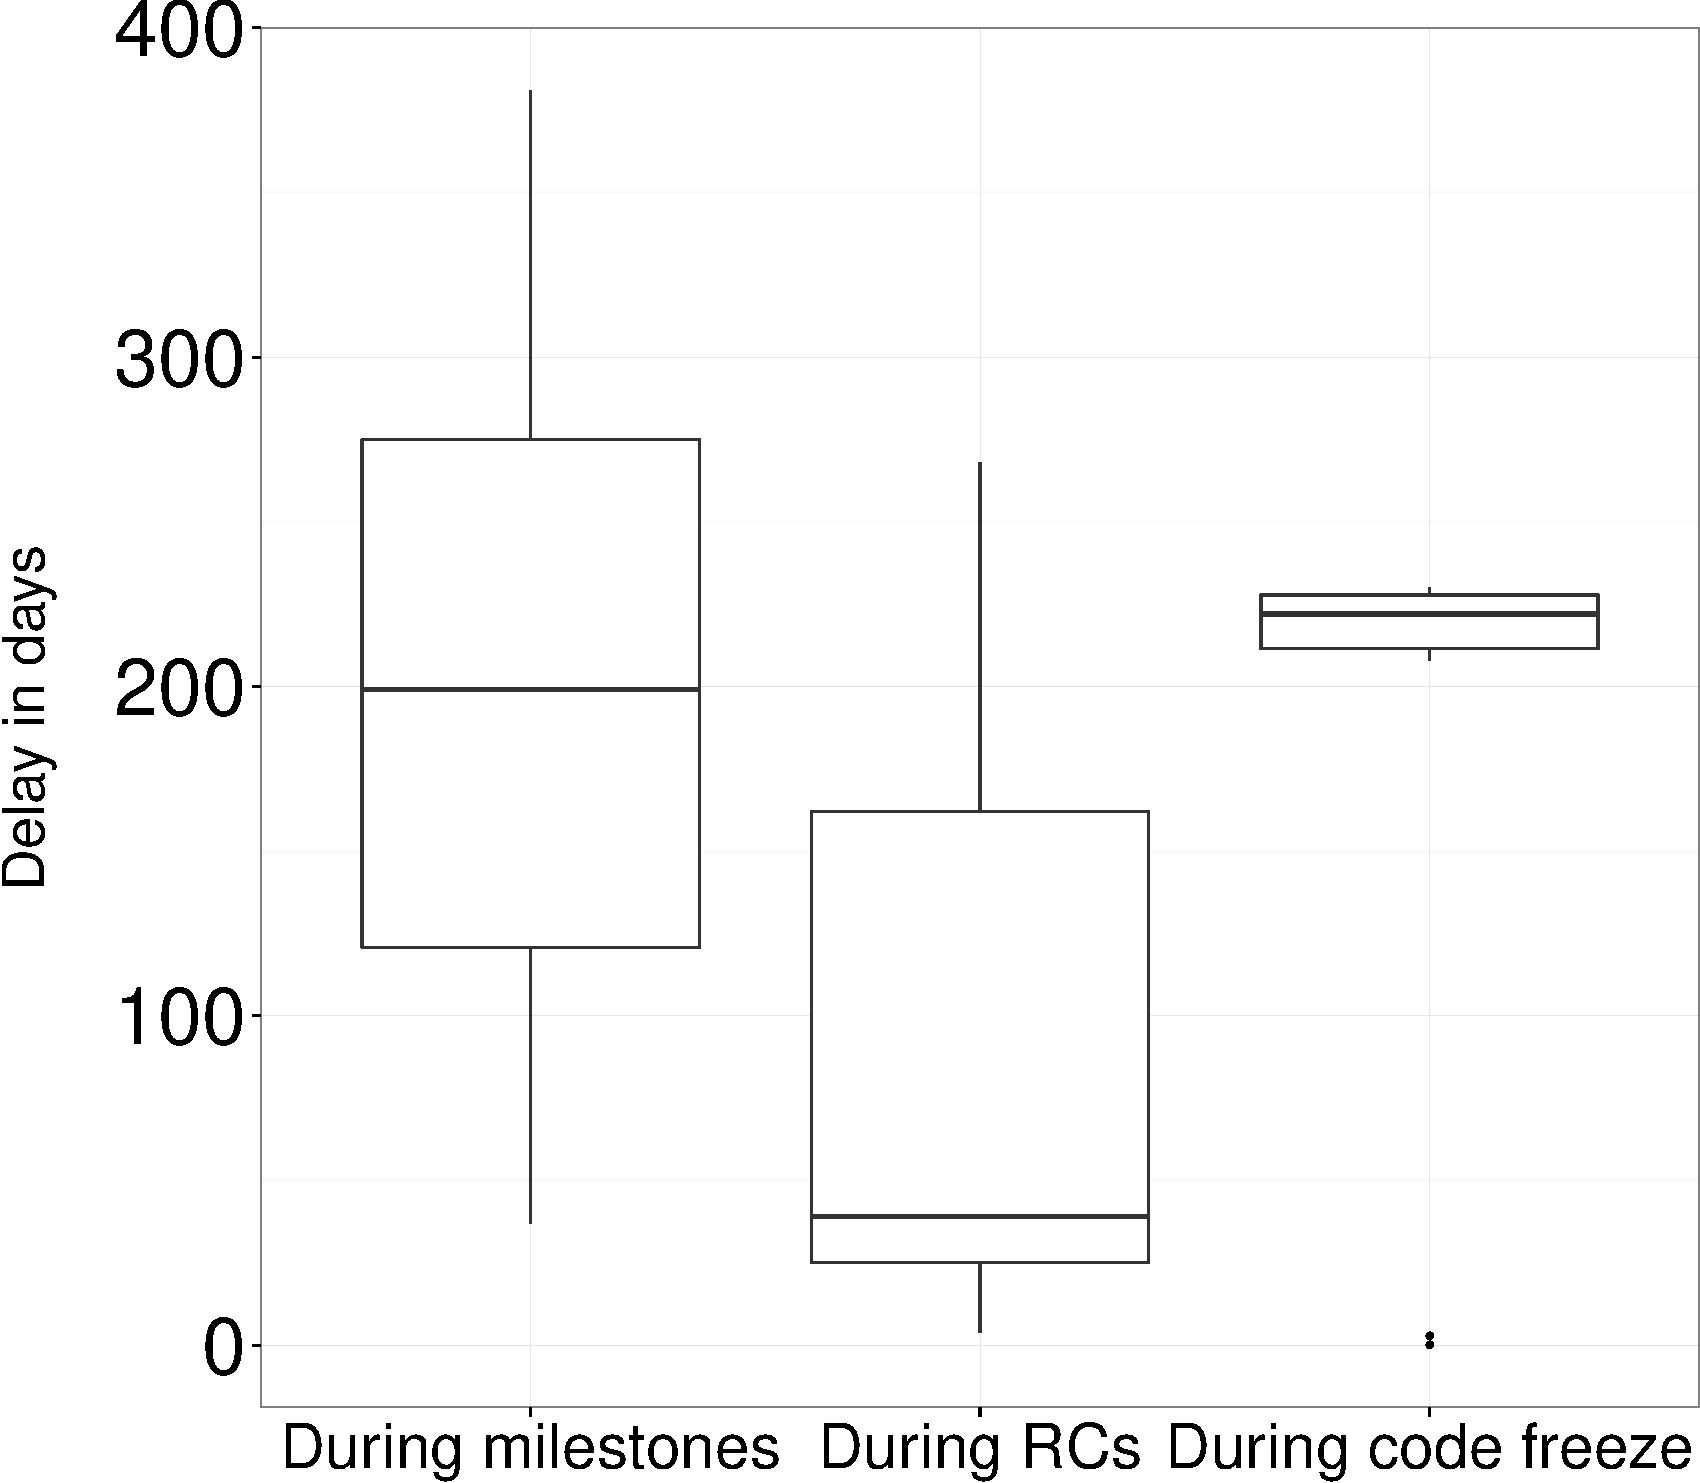
\includegraphics[width=0.50\textwidth,keepaspectratio]
		{chapters/chapter4/figures/eclipse_delay_per_stage.pdf}
	}

	\subfloat[Firefox]{
		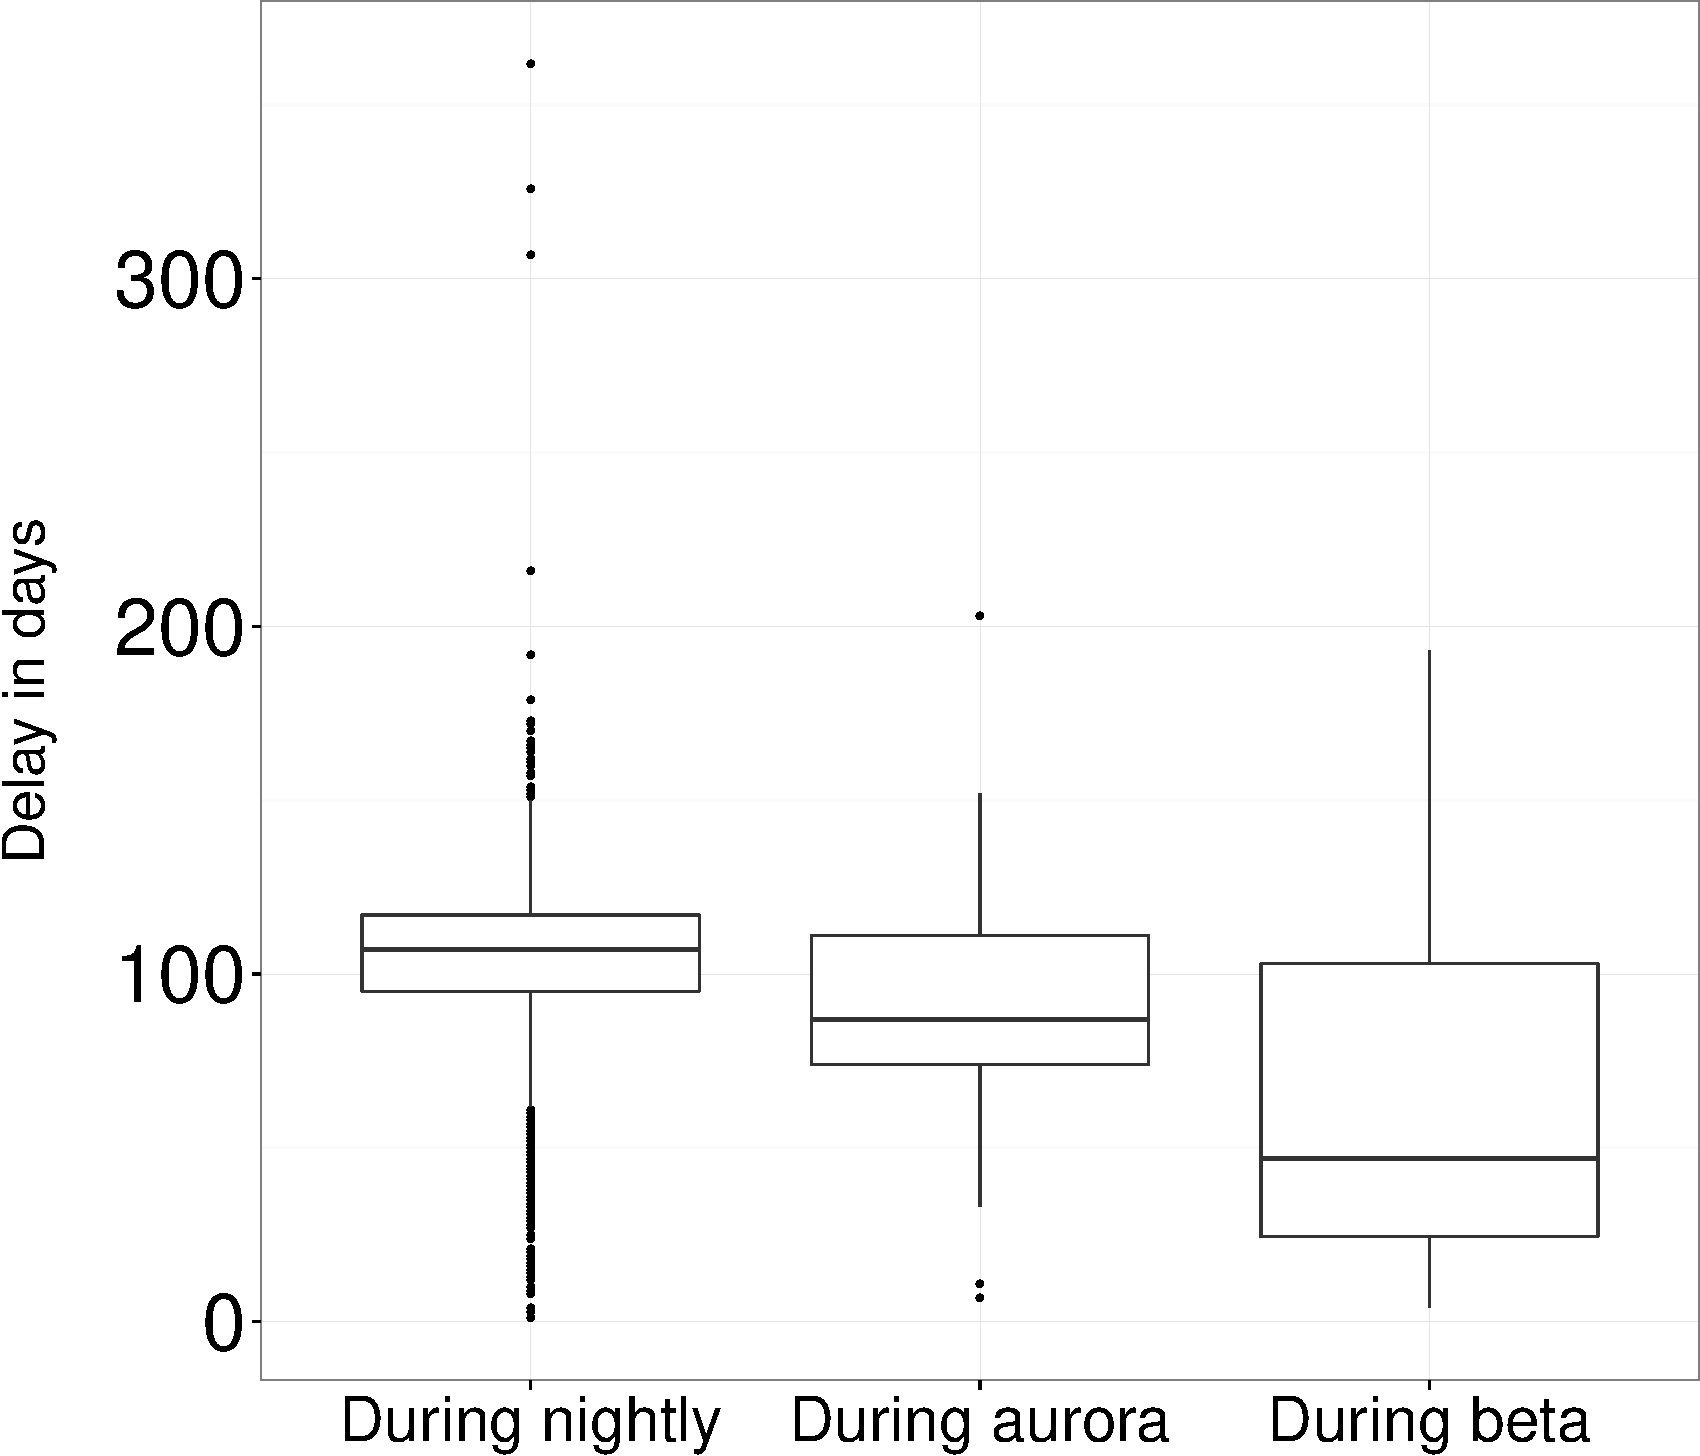
\includegraphics[width=0.50\textwidth,keepaspectratio]
		{chapters/chapter4/figures/firefox_delay_per_stage.pdf}
	}

	\subfloat[ArgoUML]{
		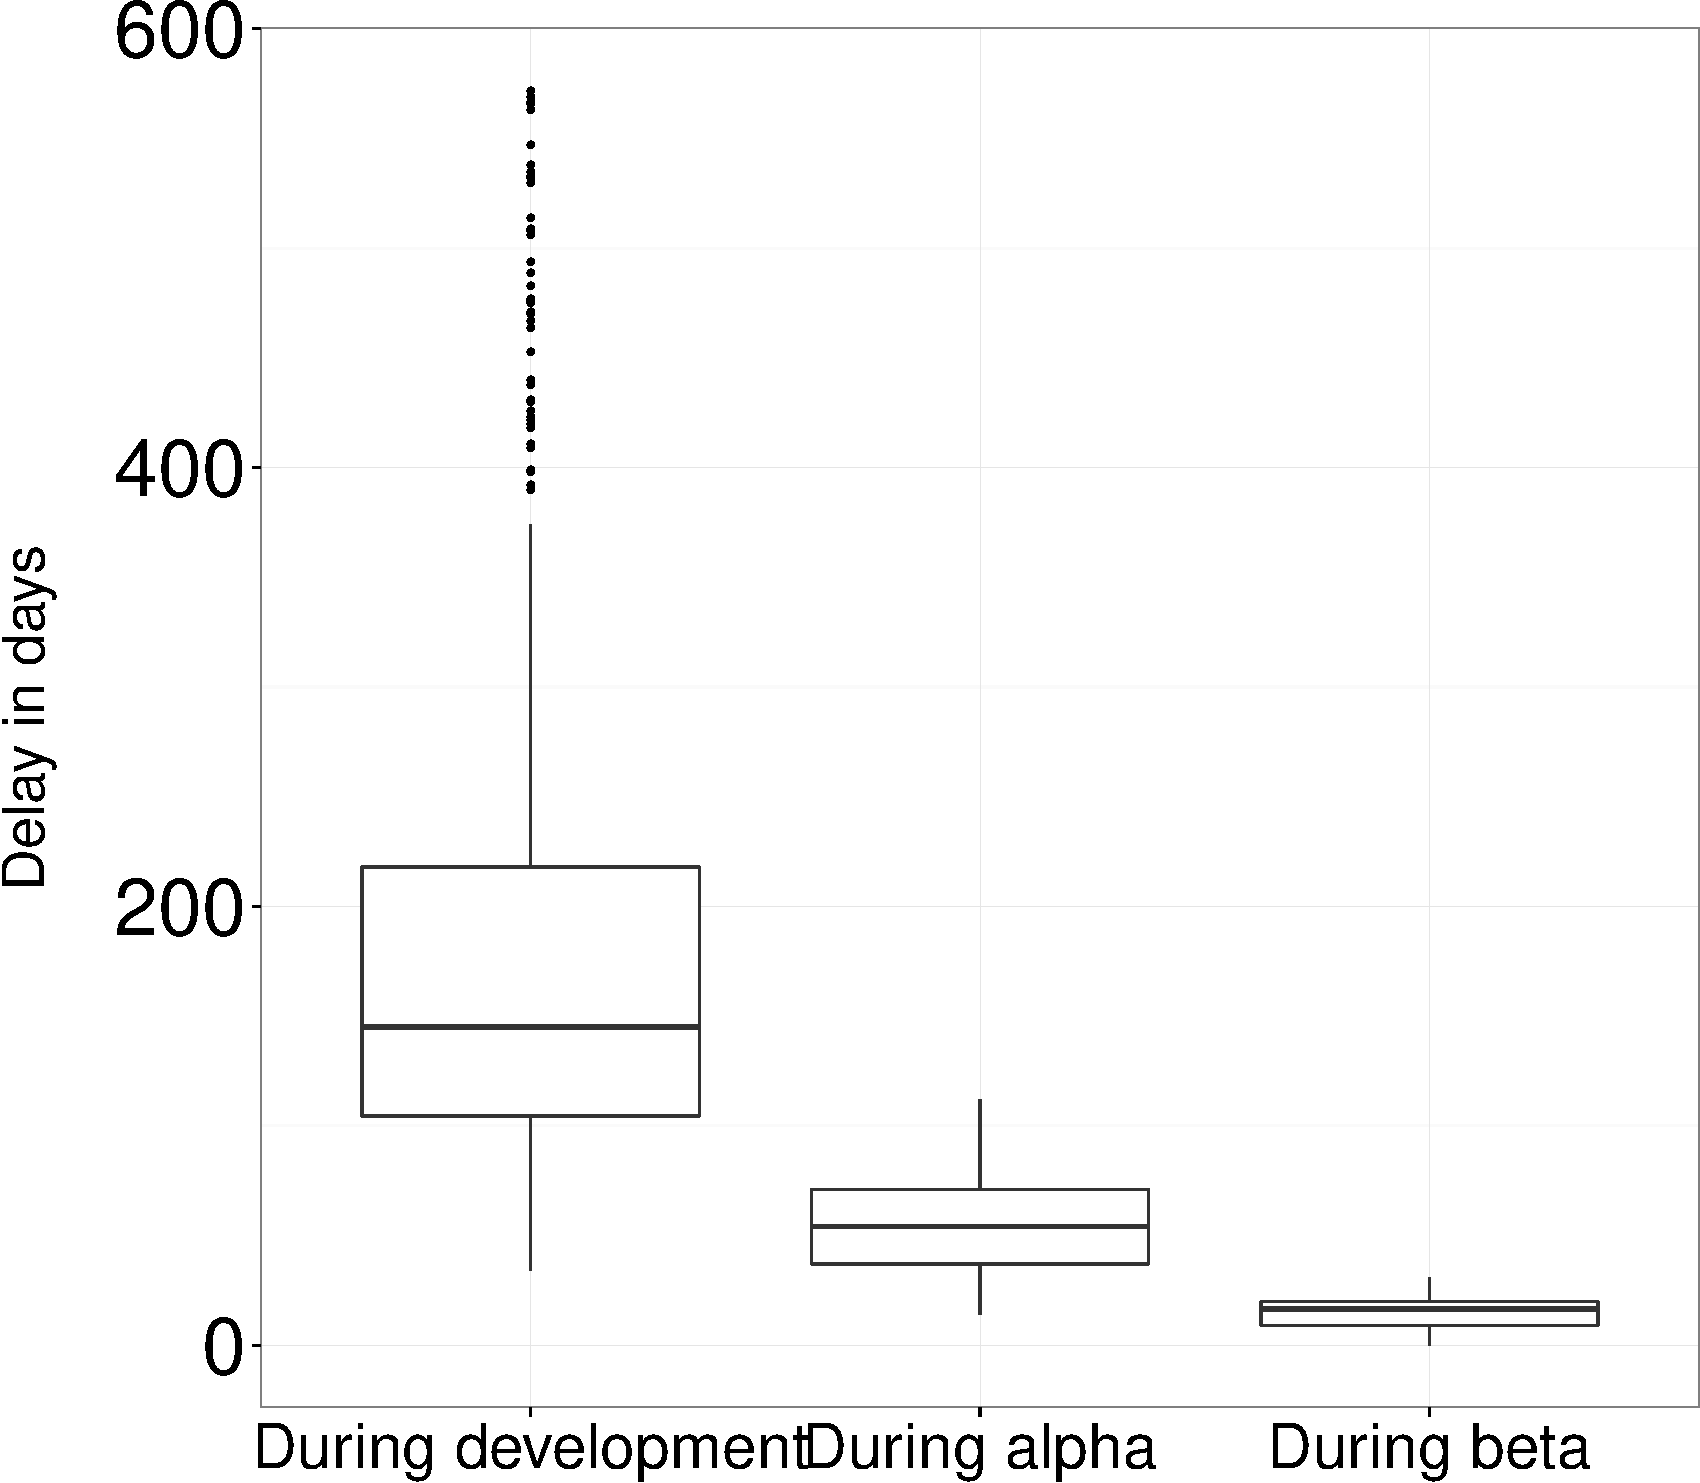
\includegraphics[width=0.50\textwidth,keepaspectratio]
		{chapters/chapter4/figures/argouml_delay_per_stage.pdf}
	}

	\caption{\textbf{delivery delay during release
		cycle stages.} Issues that are addressed during more stable stages of a release cycle
	are likely to have a shorter delivery delay}
	\label{ch4:fig:cycle_phases}
\end{figure}


\begin{table}
	\footnotesize
	\centering
	\caption{\textbf{Statistical analysis.} An overview of the $p$-$values$
		and $deltas$ that are observed during our statistical analyses.
		\label{ch4:tbl:statisticalrq2}
	}
	\resizebox{\textwidth}{!}{
		\begin{tabular}{llrrr}
			\hline 
			& \textbf{Comparison} & \textbf{Kruskal-Wallis} ($p$) &
			\textbf{Dunn} ($p.adjusted$) & \textbf{Effect-size} ($delta$)\tabularnewline
			\hline 
			\multirow{3}{*}{\textbf{Eclipse}} & Milestones vs RCs &
			\multirow{3}{*}{$1.87 \times 10^{-51}$} & $1.47 \times 10^{-52}$ & (large) $0.63$\tabularnewline
			\cline{2-2} \cline{4-5} & RCs vs Code freeze &  & $0.56$ & Not apply\tabularnewline \cline{2-2} \cline{4-5} & Milestones vs Code freeze &  & $0.02$ & (negligible) $0.09$\tabularnewline
			\hline 
			\multirow{3}{*}{\textbf{Firefox}} & Nightly vs Aurora &
			\multirow{3}{*}{$2.99 \times 10^{-76}$} & $5.07 \times 10^{-49}$ &
			(medium) $0.40$\tabularnewline
			\cline{2-2} \cline{4-5} 
			& Aurora vs Beta &  & $1.72 \times 10^{-03}$ & (medium) $0.40$\tabularnewline
			\cline{2-2} \cline{4-5} 
			& Nightly vs Beta &  & $1.43 \times 10^{-31}$ & (large) $0.57$\tabularnewline
			\hline 
			\multirow{3}{*}{\textbf{ArgoUML}} & Development vs Alpha
			& \multirow{3}{*}{$2.73 \times 10^{-135}$} & $7.24 \times 10^{-89}$
			& (large) $0.94$\tabularnewline
			\cline{2-2} \cline{4-5} 
			& Alpha vs Beta &  & $3.98 \times 10^{-09}$ & (large) $0.98$\tabularnewline
			\cline{2-2} \cline{4-5} 
			& Development vs Beta &  & $1.14 \times 10^{-78}$ & (large) $0.99$\tabularnewline
			\hline 
		\end{tabular}
	}
\end{table}

\noindent\finding{Many issues that are prevented from delivery are
addressed well before the code freeze stage of their respective release
cycle.}{find5} We compute the {\em fix timing} metric that we present in
\hyperref[rq1]{RQ1}.  However, instead of counting the number of days until an
upcoming release, we count the number of days until an upcoming code freeze
stage (\hyperref[ch4:eq:fixtiming2]{Equation}~\ref{ch4:eq:fixtiming2}). Our goal
is to check whether addressed issues are being prevented from delivery mostly
because they are being addressed too close to a code freeze stage (\ie a period
during which integration of new code changes would likely be minimal).  

\begin{figure} \center 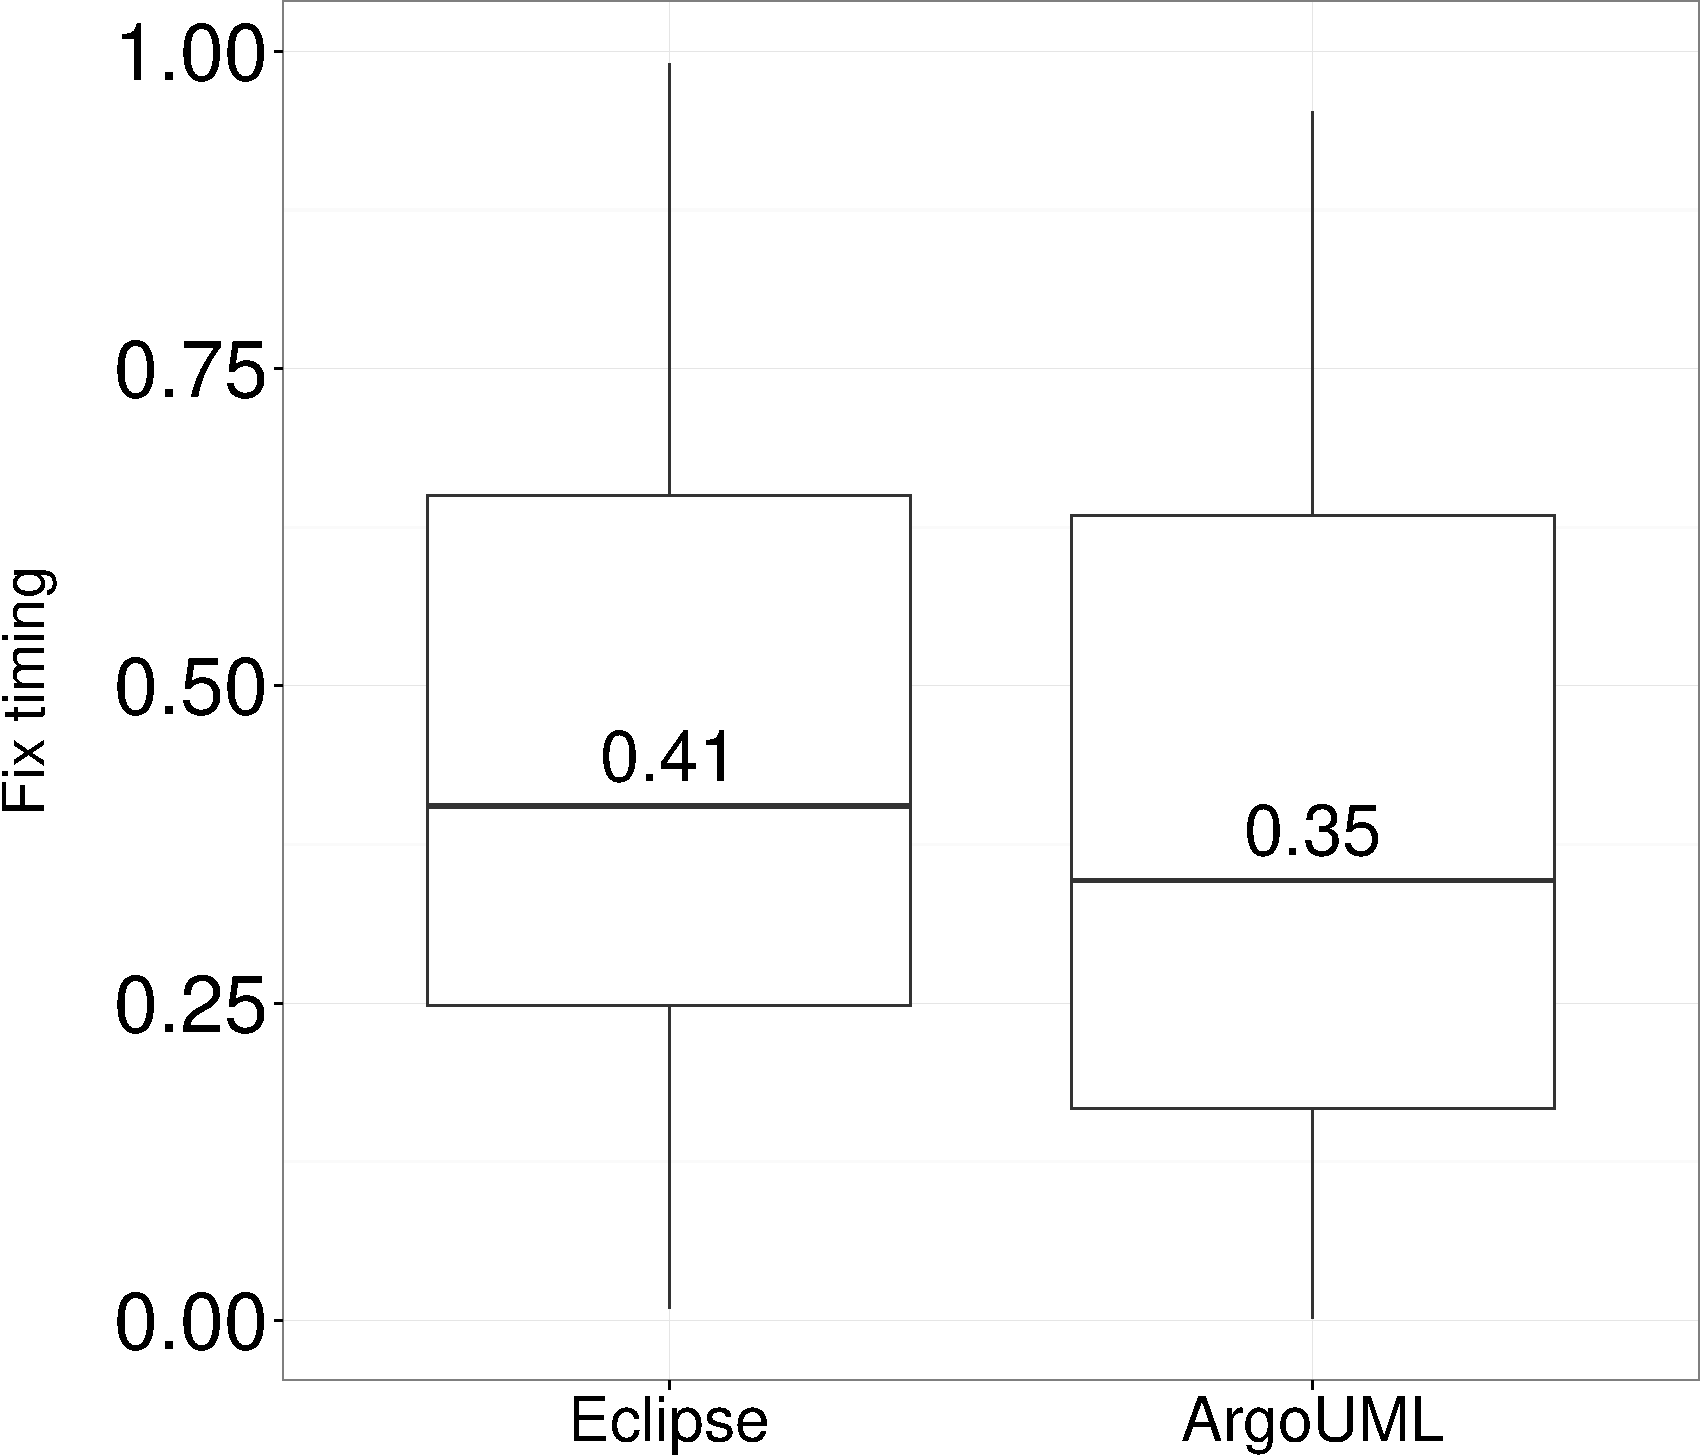
\includegraphics[width=0.60\textwidth,keepaspectratio]
	{chapters/chapter4/figures/as_codefreeze.pdf} \caption{\textbf{{\em Fix timing} values for
		the code freeze period.} The median {\em fix timing} values drop
		from 0.45 and 0.52 to 0.41 and 0.35 in the Eclipse and ArgoUML
projects, respectively. } \label{ch4:fig:codefreeze_allsystems} \end{figure}

In \hyperref[ch4:fig:codefreeze_allsystems]{Figure}~\ref{ch4:fig:codefreeze_allsystems},
we show the {\em fix timing} values for the Eclipse and ArgoUML projects, since
both projects adopt a {\em code freeze} stage. For the Eclipse project, the code
freeze starts after the last release candidate, while for the ArgoUML project,
the code freeze starts at the beginning of the {\em beta} stage (see
\hyperref[ch4:sec:subjects]{Section}~\ref{ch4:sec:subjects}). Naturally, we observe a
drop in the {\em fix timing} values, since both code freeze stages start considerably
before the official release dates. Nevertheless, we observe that even after correcting for
the code freeze stages of the Eclipse and ArgoUML projects, it is unlikely
that addressed issues are being prevented from delivery solely because of an approaching code
freeze stage. For instance, although the median {\em fix timing} for the ArgoUML project
dropped from 0.52 to 0.35, the development team would still have 2 months to
integrate an addressed issue---since the median duration of a release cycle in the
ArgoUML project is 180 days.

\conclusionbox{We observe that issues that are addressed during more stable stages of
release cycles are associated with a shorter delivery delay. We also observe
that addressed issues are unlikely to be prevented from delivery solely because
they were addressed near an upcoming code freeze stage.}

\subsection{RQ3: How well can we model the delivery delay of
addressed issues?}\label{ch4:rq3}

\subsubsection*{RQ3: Motivation} 

Several studies have proposed approaches to investigate the time that is
required to fix an issue \cite{Anbalagan2009,Giger2010, Kim2006, Marks2011,
Weib2007, Zhang2013}. These studies could help to estimate when an issue will be
addressed. However, we find that an addressed issue may be prevented from
delivery before reaching users. Even though most issues are addressed well before the next
release date, many of them are not delivered until a future release. For users
and contributors, however, knowing the delivery delay of addressed issues is of
great interest. In \hyperref[ch4:rq3]{RQ3}, we investigate if we can accurately
model delivery delay in terms of number of releases and days (\ie
\hyperref[def:1]{Definitions}~\ref{def:1} and~\ref{def:2} of delivery delay).
Our explanatory models are important to understand which attributes may impact
delivery delay of addressed issues. Moreover, such type of models could be used by
practitioners to estimate when an addressed issue will likely be delivered.

\begin{table}[t!]
	\caption{\textbf{Reporter, Resolver and Issue families.} Attributes of the
		Reporter, Resolver and Issue families that are used
		to model the delivery delay of addressed issues
		\label{ch4:tbl:dimensions}
	}
	\centering
	\footnotesize
	\begin{threeparttable}
		\begin{tabular}{rp{1.7cm}lp{9.6cm}}
			\hline
			\multicolumn{1}{c}{\textbf{Family}} &
			\multicolumn{1}{c}{\textbf{Attributes}} & \multicolumn{1}{c}{\textbf{Value}} &
			\multicolumn{1}{c}{\textbf{Definition (d)$\vert$Rationale (r)}}
			\\ \hline
			\multicolumn{ 1}{r}{\textbf{Reporter}} & Experience & Numeric & 
			\begin{tabular}{p{9.5cm}}
				\textbf{d:} Experience in filing reports for the
				project. It is measured by the number of previously
				reported issues of a reporter. \\ \hline \textbf{r:} An
				issue reported by an experienced reporter might be
				delivered quickly.
			\end{tabular}
			\\ \cline{2-4}
			\multicolumn{ 1}{r}{} & Integration speed & Numeric &
			\begin{tabular}{p{9.5cm}}
				\textbf{d:} Measured by the median integration
				time of prior issues that were reported by a
				given reporter.\\ \hline
				\textbf{r:} If issues that are reported by a
				given reporter are delivered quickly, future issues
				reported by the same reporter may also be
				delivered quickly. 
			\end{tabular}
			\\ \hline
			\multicolumn{ 1}{r}{\textbf{Resolver}} &
			$^\dagger$Experience & Numeric & 
			\begin{tabular}{p{9.5cm}}
				\textbf{d:} Experience in fixing issues for the
				project. It is measured by the number 
				of prior issues that were addressed by a given resolver.
				\\ \hline \textbf{r:} An issue that is addressed by
				an experienced resolver may be easier to
				integrate.
			\end{tabular}
			\\ \cline{2-4}
			\multicolumn{ 1}{r}{} & $^\dagger$Integration speed & Numeric &
			\begin{tabular}{p{9.5cm}}
				\textbf{d:} Measured by the median integration
				time of prior addressed issues. \\ \hline
				\textbf{r:} If the prior addressed issues of a
				particular resolver were quickly delivered,
				future issues that are addressed by the same
				resolver may also be quickly delivered. 
			\end{tabular}
			\\ \hline
			\multicolumn{ 1}{r}{\textbf{Issue}} & Component & Nominal &
			\begin{tabular}{p{9.5cm}}
				\textbf{d:} The component to which an issue is
				being reported. \\ \hline \textbf{r:} Issues that are
				related to a given component (\eg
				authentication) might be more important, and
				thus, might be delivered more quickly than issues that are
				reported to less important components.
			\end{tabular}
			\\ \cline{ 2- 4}
			\multicolumn{ 1}{r}{} & Platform & Nominal & 
			\begin{tabular}{p{9.5cm}}
				\textbf{d:} The platform specified in the issue report.
				\\ \hline \textbf{r:} Issues regarding one platform
				(\eg MS Windows) might be delivered more
				quickly than issues that are reported to
				less important platforms.
			\end{tabular}
			\\ \cline{ 2- 4}
			\multicolumn{ 1}{r}{} & Severity & Nominal &
			\begin{tabular}{p{9.5cm}}
				\textbf{d:} The severity level that
				is recorded in the issue report. \\ \hline
				\textbf{r:} severe issues (\eg
				blocking) might be delivered faster than other issues.
				Panjer observed that the severity of an issue has a
				large effect on its lifetime for the Eclipse project
				\cite{Panjer2007}.
			\end{tabular}
			\\ \cline{ 2- 4}
			\multicolumn{ 1}{r}{} & Priority & Nominal &
			\begin{tabular}{p{9.5cm}}
				\textbf{d:} The priority that is assigned to the
				issue report. \\ \hline
				\textbf{r:} High priority issues will likely be
				delivered before low priority issues. 
			\end{tabular}
			\\ \cline{2- 4}
			\multicolumn{ 1}{r}{} & $^\dagger$Stack trace attached & Boolean & 
			\begin{tabular}{p{9.5cm}}
				\textbf{d:} We check whether the issue report has a stack
				trace attached in its description. \\ \hline \textbf{r:}
				A stack trace attached in the description of the issue report may provide
				useful information with respect to the cause of the issue, which
				may quicken the delivery of that addressed issue
				\cite{schroter2010stack}.
			\end{tabular}
			\\ \cline{2-4}
			\multicolumn{ 1}{r}{} & Description Size & Numeric &
			\begin{tabular}{p{9.5cm}}
				\textbf{d:} Description of the issue measured by
				the number of words in its description. \\
				\hline \textbf{r:} Issues that are
				well-described might be easier to integrate than
				issues that are difficult to understand. 
			\end{tabular}
			\\ \hline
		\end{tabular}
		\begin{tablenotes}
		\item[$\dagger$] New attributes that did not appear in our
			previous work \cite{costa2014empirical}
		\end{tablenotes}
	\end{threeparttable}
\end{table}

\begin{table}[t!]
	\caption{\textbf{Project family.} Attributes of the
		Project family that is used
		to model the delivery delay of an addressed issue.
		\label{ch4:tbl:dimensions2}
	}
	\centering
	\footnotesize
	\begin{threeparttable}
		\begin{tabular}{rp{2.3cm}lp{9cm}}
			\hline
			\multicolumn{1}{c}{\textbf{Family}} &
			\multicolumn{1}{c}{\textbf{Attributes}} & \multicolumn{1}{c}{\textbf{Value}} &
			\multicolumn{1}{c}{\textbf{Definition (d)$\vert$Rationale (r)}}
			\\ \hline
			\multicolumn{ 1}{r}{\textbf{Project}} & Backlog of
			issues & Numeric &
			\begin{tabular}{p{8.9cm}}
				\textbf{d:} The number of issues in the RESOLVED-FIXED
				state at a given time. \\ \hline \textbf{r:} Having a
				large number of addressed issues at a given time might
				create a high workload on team members, which may affect
				the number of addressed issues that are delivered.
			\end{tabular}
			\\ \cline{ 2- 4}
			\multicolumn{ 1}{r}{} & $^\dagger$Queue position  & Numeric & 
			\begin{tabular}{p{8.9cm}}
				\textbf{d:} $\frac{\text{rank of the
				issue}}{\text{all addressed issues}}$, where the
				rank is the position in time at which an issue
				was addressed in relation to others in the current
				release cycle. The rank is divided by all of the
				issues that were addressed until the end of the
				current release cyle. \\ \hline \textbf{r:} An
				issue that is near the front of the queue is
				more likely to be quickly delivered.
			\end{tabular}                       
			\\ \hline
			\multicolumn{ 1}{r}{} & $^\dagger$Fixing time per
			resolver & Numeric & 
			\begin{tabular}{p{8.9cm}}
				\textbf{d:} $\frac{\sum\limits_{issue=1}^{total} \text{fixing
				time}}{\text{\# of resolvers}}$, the sum of the
				time (measured in terms of days)
				to fix the issues of the current release
				cycle over the number of resolvers that worked
				in that release cycle~\cite{mythical}. \\ \hline
				\textbf{r:} The higher the total fixing time
				that is spent per resolver in fixing issues the
				less the likelihood of an addressed issue
				experiencing a large delivery delay.
			\end{tabular}                       
			\\ \hline
			\multicolumn{ 1}{r}{} & $^\dagger$Backlog of issues per
			resolver& Numeric & 
			\begin{tabular}{p{8.9cm}}
				\textbf{d:} The number of issues in the
				RESOLVERD-FIXED state at a given time for each
				resolver of the development team. \\ \hline
				\textbf{r:} Having a large number of addressed
				issues per resolver might create a workload on
				that resolver to integrate the issue.
			\end{tabular}                       
			\\ \hline
		\end{tabular}
		\begin{tablenotes}
		\item[$\dagger$] New attributes that did not appear in our previous
			work \cite{costa2014empirical}
		\end{tablenotes}
	\end{threeparttable}
\end{table}

\begin{table}[t!]
	\caption{\textbf{Process family.} Attributes of the
		Process family that is used
		to model the delivery delay of an addressed issue.
		\label{ch4:tbl:dimensions3}
	}
	\centering
	\footnotesize
	\begin{threeparttable}
		\begin{tabular}{rp{2.3cm}lp{9cm}}
			\hline
			\multicolumn{1}{c}{\textbf{Family}} &
			\multicolumn{1}{c}{\textbf{Attributes}} & \multicolumn{1}{c}{\textbf{Value}} &
			\multicolumn{1}{c}{\textbf{Definition (d)$\vert$Rationale (r)}}
			\\ \hline
			\multicolumn{ 1}{r}{\textbf{Process}} & Number of Impacted Files & Numeric & 
			\begin{tabular}{p{8.9cm}}
				\textbf{d:} The number of files that are linked to an issue
				report. \\ \hline \textbf{r:} delivery delay
				might be related to a high number of impacted files
				because more effort would be required to properly
				integrate code modifications \cite{Jiang2013}. 
			\end{tabular}
			\\ \cline{ 2- 4}
			\multicolumn{ 1}{r}{} & Number of Activities & Numeric &
			\begin{tabular}{p{8.9cm}}
				\textbf{d:} An activity is an entry in the issue's
				history. \\ \hline \textbf{r:} A high number of
				activities might indicate that much work was necessary
				to fix the issue, which can impact the delivery
				delay of an issue.~\cite{Jiang2013}. 
			\end{tabular}
			\\ \cline{ 2- 4}
			\multicolumn{ 1}{r}{} & Number of Comments & Numeric &
			\begin{tabular}{p{8.9cm}}
				\textbf{d:} The number of comments of an issue report.
				\\ \hline \textbf{r:} A large number of comments might
				indicate the importance of an issue or the difficulty
				to understand it~\cite{Giger2010}, which might impact
				delivery delay~\cite{Jiang2013}. 
			\end{tabular}
			\\ \cline{ 2- 4}
			\multicolumn{ 1}{r}{} & Number of Tosses & Numeric &
			\begin{tabular}{p{8.9cm}}
				\textbf{d:} The number of times that the issue's assignee has
				changed. \\ \hline \textbf{r:} The number of changes in
				the issue assignee might indicate a complex issue to
				fix or a difficulty in understanding such an issue,
				which can impact delivery delay. One of the
				reasons for changing the assigned developer is because
				additional expertise may be required to fix 
				an issue \cite{Jiang2013,Jeong2009}. 
			\end{tabular}
			\\ \cline{2-4}
			\multicolumn{ 1}{r}{} & Comment Interval & Numeric &
			\begin{tabular}{p{8.9cm}}
				\textbf{d:} The sum of all of the time intervals
				between comments (measured in hours) divided by the
				total number of comments. \\ \hline \textbf{r:} A short
				comment time interval indicates that an active
				discussion took place, which suggests that the issue is
				important.
				\cite{Jiang2013}. 
			\end{tabular}
			\\ \cline{2-4}
			\multicolumn{ 1}{r}{} & Churn & Numeric &
			\begin{tabular}{p{8.9cm}}
				\textbf{d:} The sum of the added lines and removed
				lines in the code repository. \\ \hline \textbf{r:} A
				higher churn suggests that a great amount of work was
				required to fix the issue, and hence, verifying the
				impact of integrating the modifications may also be
				difficult \cite{Nagappan2005, Jiang2013}.
			\end{tabular}
			\\ \cline{2-4}
			\multicolumn{ 1}{r}{} & $^\dagger$Fixing time & Numeric &
			\begin{tabular}{p{8.9cm}}
				\textbf{d:} The number of days between the
				moment at which an issue is opened the moment at
				which the issue is addressed (\ie the issue reaches
				the RESOLVED-FIXED status) \cite{Giger2010}. \\ \hline
				\textbf{r:} Issues that are addressed quickly might
				indicate that the necessary code changes are
				easy to integrate, wich may quicken delivery delay. 
			\end{tabular}
			\\ \hline
		\end{tabular}
		\begin{tablenotes}
		\item[$\dagger$] New attributes that did not appear in our previous
			work \cite{costa2014empirical}
		\end{tablenotes}
	\end{threeparttable}
\end{table}

\subsubsection*{RQ3: Approach} 

In order to study when an addressed issue is delivered, we collect information from
both the ITSs and VCSs of the studied systems. We train models using attributes
that are grouped in the following families: \textit{reporter},
\textit{resolver}, \textit{issue}, \textit{project}, and \textit{process}.
\begin{itemize}
	\item \textbf{Reporter:} refers to the attributes regarding an issue reporter.
		Issues that are reported by a reporter who is known to report important
		issues may receive more attention from the integration team.\\

	\item \textbf{Resolver:} refers to team members that fix issues.
		Issues that are addressed by experienced resolvers may be easier
		to integrate and ship to end users.\\

	\item \textbf{Issue:} refers to the attributes of issues reports. Project teams use this
		information to triage, fix, and integrate issues. For
		example, integrators may not be able to properly assess the
		importance and impact of poorly described issues, which may
		increase delivery delay.\\

	\item \textbf{Project:} refers to the status of the project when a
		specific issue is addressed. If the project team has a heavy
		integration workload, \ie many addressed issues waiting to be
		delivered, the delivery of newly addressed issues may be
		hindered.\\

	\item \textbf{Process:} refers to the process of fixing an issue. An
		addressed issue that involved a complex process (\eg long comment
		threads, large code changes) could be more difficult to
		understand and integrate.\\
\end{itemize}

\hyperref[ch4:tbl:dimensions]{Tables}~\ref{ch4:tbl:dimensions},
\ref{ch4:tbl:dimensions2} and~\ref{ch4:tbl:dimensions3} describe the attributes
that we compute for each family. For each attribute,
\hyperref[ch4:tbl:dimensions]{Tables}~\ref{ch4:tbl:dimensions},
\ref{ch4:tbl:dimensions2} and~\ref{ch4:tbl:dimensions3} present our rationale
for using it in our models. We choose these families of attributes because (i)
we intend to study a variety of perspectives that might influence delivery delay
and (ii) they are simple to compute using the publicly available data sources
(\eg ITSs and VCs) from our studied systems.

We train exploratory models to study how many releases an addressed issue is likely
to be prevented from delivery (\hyperref[def:1]{Definition}~\ref{def:1}). To
study delivery delay in terms of releases, we use the \textit{random forest}
classification technique \cite{RandomForest2001}. Random forest is an {\em
ensemble learning} technique that operates by combining a multitude of decision
trees at the training stage.  Each decision tree uses a random subset of the
attributes that are used to explain one phenomenon (\eg delivery delay). Next,
each decision tree votes for the response bucket (\eg {\em next} or {\em after-1}
release(s)) of a given instance. The majority of the votes for a given bucket
will be the actual response of the random forest. We choose random forests
because they are known to have a good overall accuracy and to be robust to
outliers as well as noisy data. Model robustness is important for our study
because the data in the ITSs tend to be noisy~\cite{Herraiz2008}. In our study,
we use the \textit{random forest} implementation provided by the \textit{bigrf}
R package.\smartfoot{Bigrf package \url{https://cran.r-project.org/src/contrib/Archive/bigrf/}} 

Since our data has a temporal order, \ie the values of the attributes for each
instance depends on the time at which the issue was addressed, we evaluate our
models by adapting the {\em Leave One Out Cross Validation} (LOOCV) technique.
In our LOOCV variation, we first sort the data by the date at which the issues
were addressed. Then, we train models to predict each next instance of the data. For
example, if issue $A$ is addressed before issue $B$, we train a model using $A$ and
test it using $B$. Furthermore, if issues $A$ and $B$ are addressed before $C$, we
train a model using $A$ and $B$ and test it using $C$. This process is repeated
until we test a model by using the last addressed issue in our data.

We evaluate the performance of our random forest models using the
\textit{precision}, \textit{recall}, \textit{F-measure}, and \textit{AUC}. We
also use \textit{Zero-R} models as a baseline to compare the results of our
models, since no prior models have been proposed to model delivery delay. We
describe each one below.

\textit{Precision} (P) measures the correctness of our models in estimating the
number of releases that are necessary to ship an addressed issue. An estimation is
considered correct if the estimated delivery delay is the same as the actual
delivery delay of an addressed issue. Precision is computed as the proportion of
correctly estimated delivery delay for each studied delivery delay bucket (\eg
next, after-1).

\textit{Recall} (R) measures the completeness of a model. A model is considered
complete if all of the addressed issues that were delivered in a given release
\(r\) are estimated to appear in \(r\).  Recall is computed as the proportion of
issues that actually appear in a release \(r\) that were correctly estimated as
such.

\textit{F-measure} (F) is the harmonic mean of precision and recall, (\ie $\frac
{2 \times P \times R}{P + R}$). F-measure combines the inversely related
precision and recall values into a single descriptive statistic. 

\textit{Area Under the Curve} (AUC) is used to evaluate the degree of
discrimination achieved by the model \cite{hanley1982meaning}. For instance, AUC
can be used to evaluate how well our models can distinguish between addressed issues
that are prevented from delivery into one or two releases. The AUC is the
area below the curve plotting the true positive rate against false positive
rate. The value of AUC ranges between 0 (worst) and 1 (best). An area greater
than 0.5 indicates that the explanatory model outperforms a random predictor. We
computed the AUC value for a given bucket \(b\) (\eg \textit{next}) on a binary
basis. In other words, the probabilities of the instances were analyzed as
pertaining to a given bucket \(b\) or not. For example, when computing the AUC
value for the \textit{next} bucket, the AUC value is computed by verifying if an
instance belongs to the \textit{next} bucket or not. This process is repeated
for each bucket. Therefore, each bucket has its own AUC value.  

\textit{Zero-R models} are na\"{i}ve models that always select the bucket with
the highest number of instances. For example, a Zero-R model trained with the
Firefox project data would always select \textit{after-2} as the response for
each instance. 

We also study the delivery delay in terms of number of days
(\hyperref[def:2]{Definition}~\ref{def:2}). We train linear regression models
(using the \textit{ordinary least squares} technique~\cite{springertexts}) to
study delivery delay in terms of days. Linear regression is an approach for
modeling relationships between a dependent variable $y$ and one or more
explanatory variables $x$. When a single explanatory variable is used, the
approach is called {\em simple linear regression}, whereas when several
explanatory variables are used, the approach is called {\em multiple linear
regression}~\cite{freedman2009statistical}.  Regression models fit a curve of
the form $y = \beta_0 + \beta_{1}X_1 + \beta_{2}X_2 + ... + \beta_{n}X_n$. The
$y$ variable is the response variable (\ie delivery delay in terms of days in
our case), while the set of ${X}$ variables represent explanatory variables that
may share a relationship with $y$. The set of $\boldsymbol{\beta}$ coefficients
represent weights given by the model to adjust the values of $X$ to better
estimate the response $y$. The set of explanatory variables that we use in our
study are the attributes that are outlined in
\hyperref[ch4:tbl:dimensions]{Tables}~\ref{ch4:tbl:dimensions},~\ref{ch4:tbl:dimensions2}~and~\ref{ch4:tbl:dimensions3}.  

\begin{figure}
	\centering
	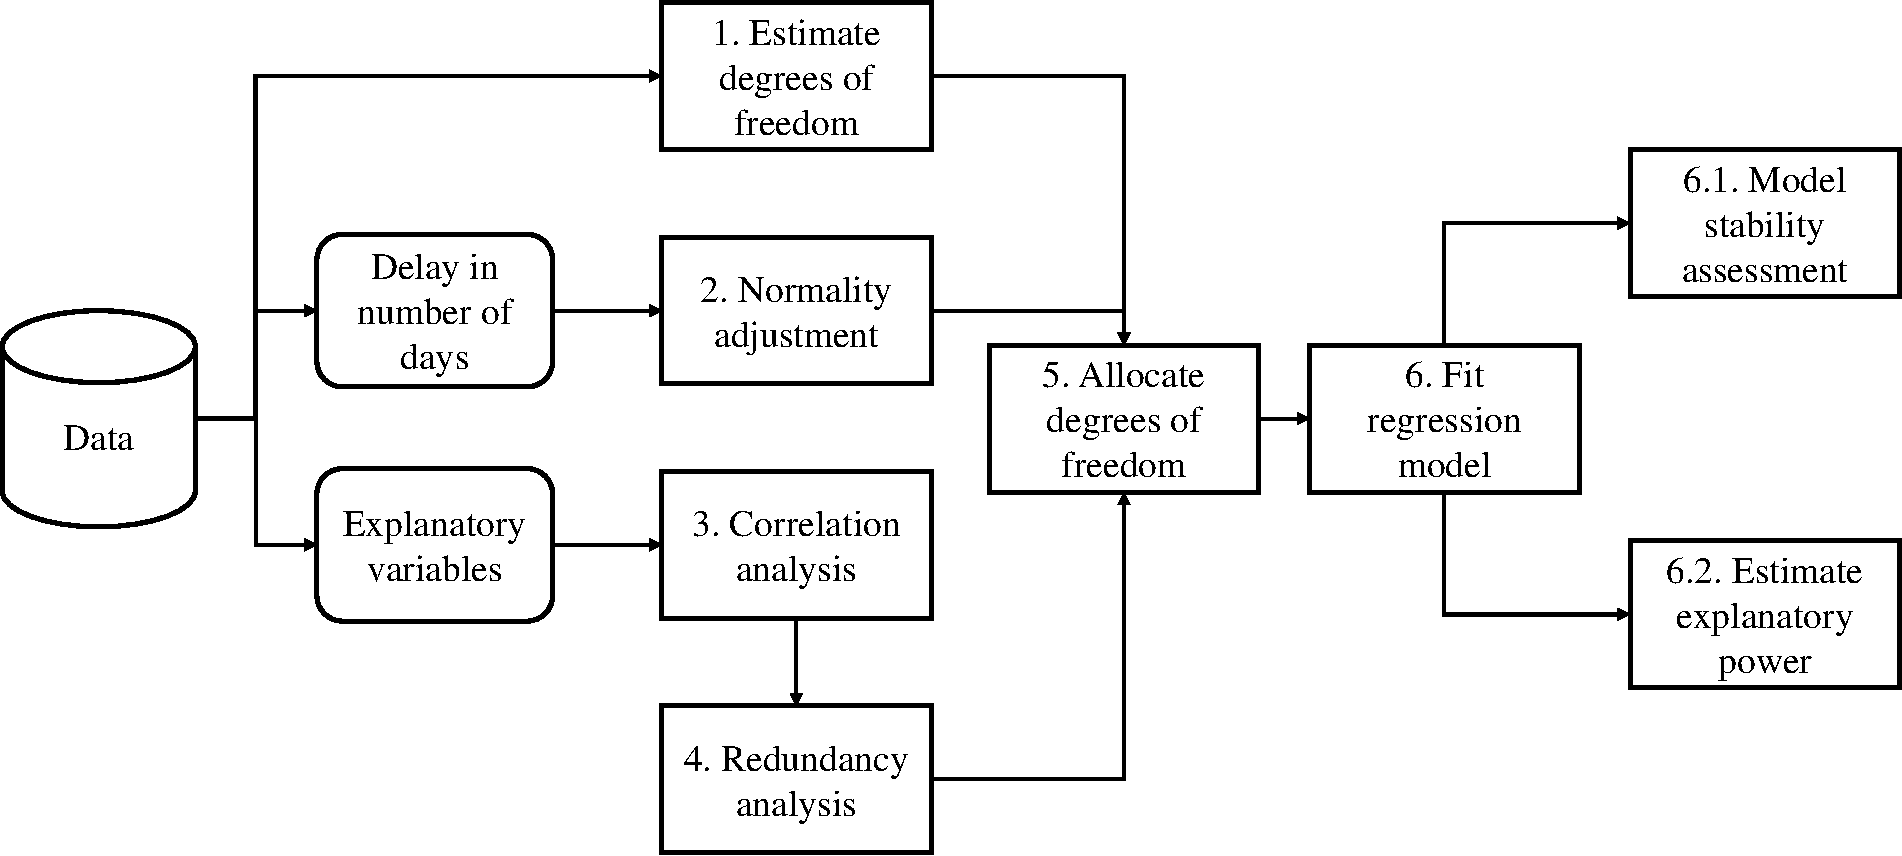
\includegraphics[width=\textwidth,keepaspectratio]
	{chapters/chapter4/figures/linear_model_building_overview}
	\caption{\textbf{Training regression models.} We follow the guidelines
		that are
		provided by Harrell~Jr.~\cite{harrell2001regression} to train regression models, which
	involves nine activities, from data collection to model validation. The
results of Steps 6.2 and is presented in \hyperref[ch4:rq4]{RQ4}.}
	\label{ch4:fig:regression_process}
\end{figure}

We use the guidelines that are provided by
Harrell~Jr.~\cite{harrell2001regression} to fit our regression models.
\hyperref[ch4:fig:regression_process]{Figure}~\ref{ch4:fig:regression_process} provides
an overview of our model fitting approach. In Step~1, we compute the budget of
degrees of freedom that our data can accommodate while keeping the risk of
overfitting low. We compute this budget by using the formula $\frac{n}{15}$
(where $n$ is the number of issues in our dataset). In Step~2, we verify the
normality assumption of \textit{ordinary least squares}, \ie it assumes that the
response variable $y$ should follow normal distribution. Through analysis of the
delivery delay values (\ie the $y$ variable), we find that it does not follow
a normal distribution, and hence, we apply a log transformation $[ln(y+1)]$ to
mitigate such skewness.

In Step~3, we use a variable clustering analysis~\cite{sarle1990varclus} to
remove highly correlated variables. For variables within a cluster that have a
correlation of $|\rho|>0.7$, we choose only one of them to include in our
models---we choose the variable with the least skewed distribution and that we
suspect that shares a stronger relationship with delivery delay. In Step~4, we
check the redundancy of the surviving explanatory variables. Redundant variables
do not add explanatory power to the models and can distort the relationship
between explanatory and response variables. To remove redundant variables we use
the \code{redun} function from the \code{rms} R package, which fits models to
explain each explanatory variable using the other explanatory variables. We then
discard those explanatory variables that could be estimated with an $R^2 \geq
0.9$ (the default threshold of the \code{redun} function).

In the following step (Step~5), we identify which explanatory variables may
benefit from a relaxation of the linear relationship with the response variable.
To identify such variables, we calculate the Spearman multiple $\rho^2$ between
the response and explanatory variables. We spend more of our budgeted degrees of
freedom on the explanatory variables that obtain the higher $\rho^2$ values.

In Step~6, we fit our regression models. In order to assess the fit of our
models (Step~6.1) we use the $R^2$ metric. The $R^2$ measures the {\em
``variability explained''} of the dependent variable that is
analyzed~\cite{steel1960principles}. For instance, a $R^2$ of 0.4 indicates that
40\% of the variability of the dependent variable is being modeled ({\em
``explained''}) by the explanatory variables---the remaining 60\% of the
variability may be due to external factors that are not being modeled or cannot
be controlled. 
%The interpretation of $R^2$ values depends on the analysis that is being
%performed. For example, when prediction is the main goal, the $R^2$ values
%should be very high (\eg around 0.7 to 0.9)~\cite{choi2012predicting}. On the
%other hand, low $R^2$ values (\eg around 0.20) may also generate important
%insights in fields such as psychology or social
%sciences~\cite{bersani2016association}. 

We also use the \textit{Mean Absolute Error} (MAE) to verify how close are the
estimates of our models ($\hat{y}$) to the actual observations ($y$). Then, we
assess the stability of our models by using the \textit{bootstrap-calculated
optimism} of the $R^2$. The \textit{bootstrap-calculated optimism} is computed
by fitting models using bootstrap samples of the original data. For each model
fit to a bootstrap sample, we subtract the $R^2$ of such a model from the model
fit to the original data. This difference is a measure of the \textit{optimism}
in the original model. In this work, we obtain the \textit{bootstrap-calculated
optimism} by computing the average \textit{optimism} obtained using 1,000
bootstrap samples. The smaller the \textit{bootstrap-calculated optimism} the
more stable are our models~\cite{efron1986biased}.

\subsubsection*{\textit{\textbf{RQ3: Results for delivery delay in terms of
releases}}}

\noindent\finding{Our explanatory models obtain a median precision of 0.81 to
0.88 and a median recall of 0.29 to 0.92.}{find6}
\hyperref[ch4:fig:RFclassificationResult]{Figure}~\ref{ch4:fig:RFclassificationResult}
shows the precision, recall, F-measure, and AUC of our explanatory models.  The
bar charts show the values that we observe for each bucket. The values of
precision, recall, F-measure, and AUC are also shown in
\hyperref[ch4:tbl:evaluation_metrics]{Table}~\ref{ch4:tbl:evaluation_metrics}. 

\begin{figure}
	\centering
	%\captionsetup{justification=centering}
	\subfloat[Eclipse]{
		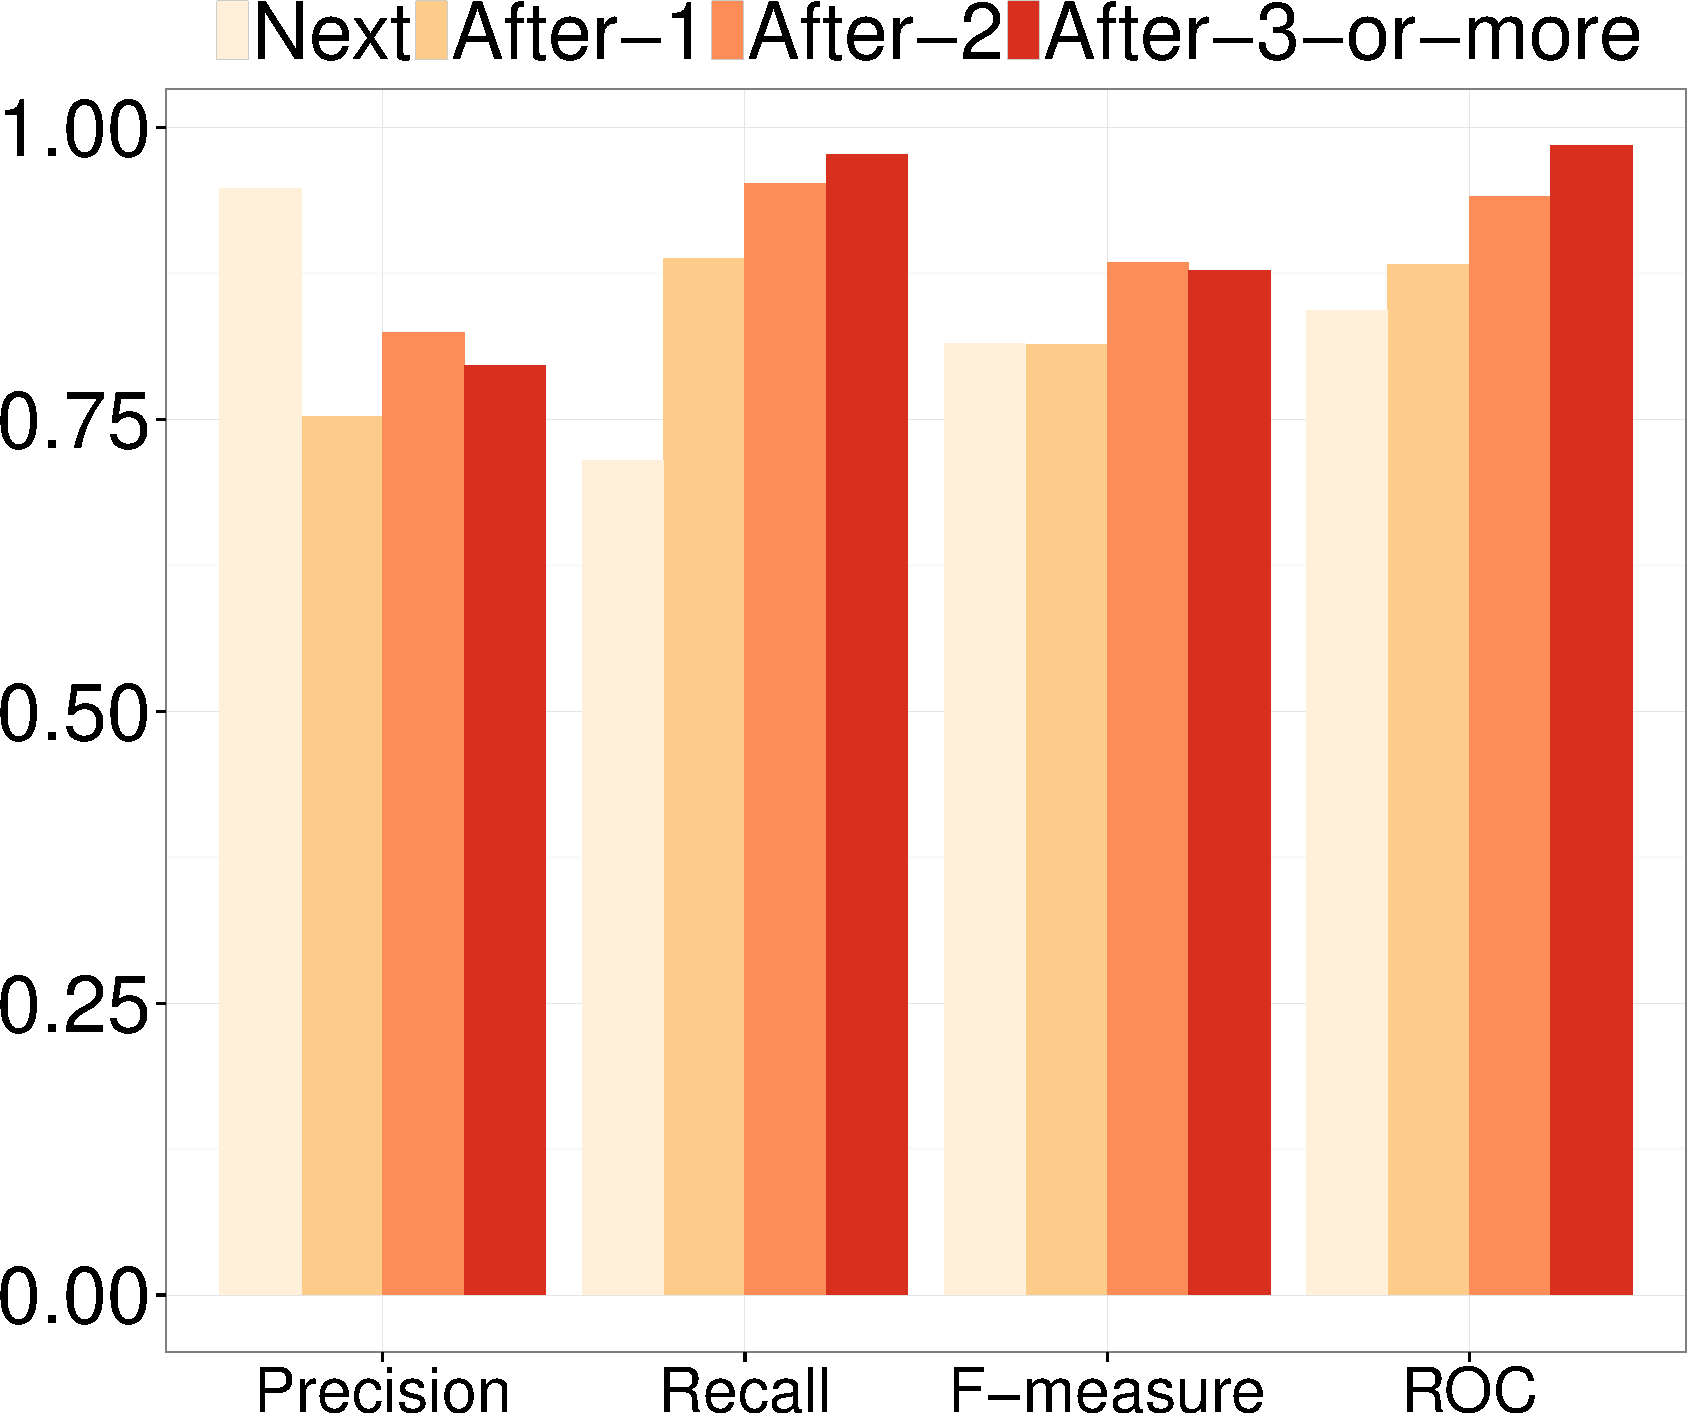
\includegraphics[width=0.50\textwidth,keepaspectratio] 
		{chapters/chapter4/figures/eclipse_loocv_evaluation.pdf}
		\label{ch4:fig:RFeclipse}
	}

	\subfloat[Firefox]{
		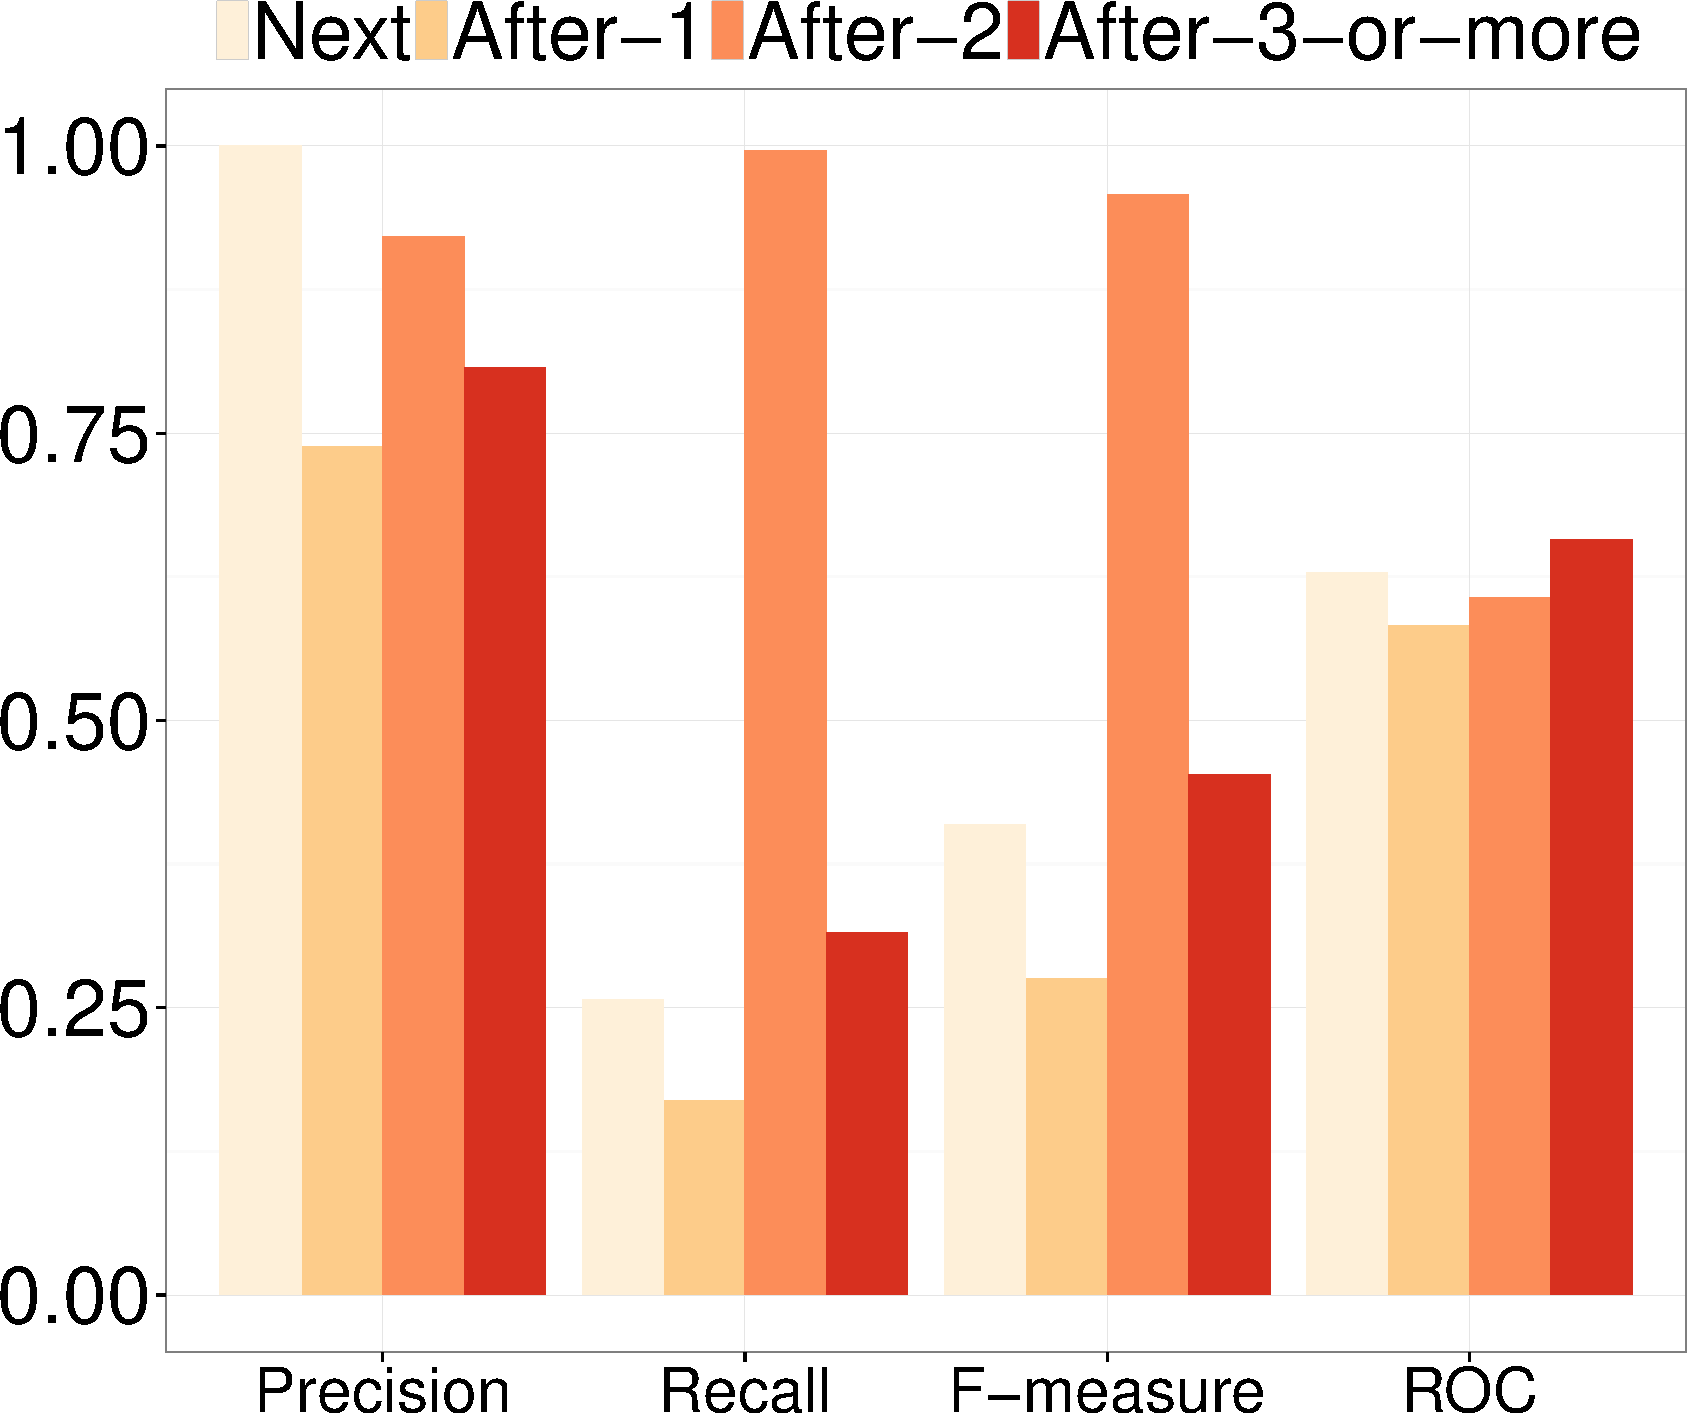
\includegraphics[width=0.50\textwidth,keepaspectratio]  
		{chapters/chapter4/figures/firefox_loocv_evaluation.pdf}
		\label{ch4:fig:RFfirefox}
	}

	\subfloat[ArgoUML]{
		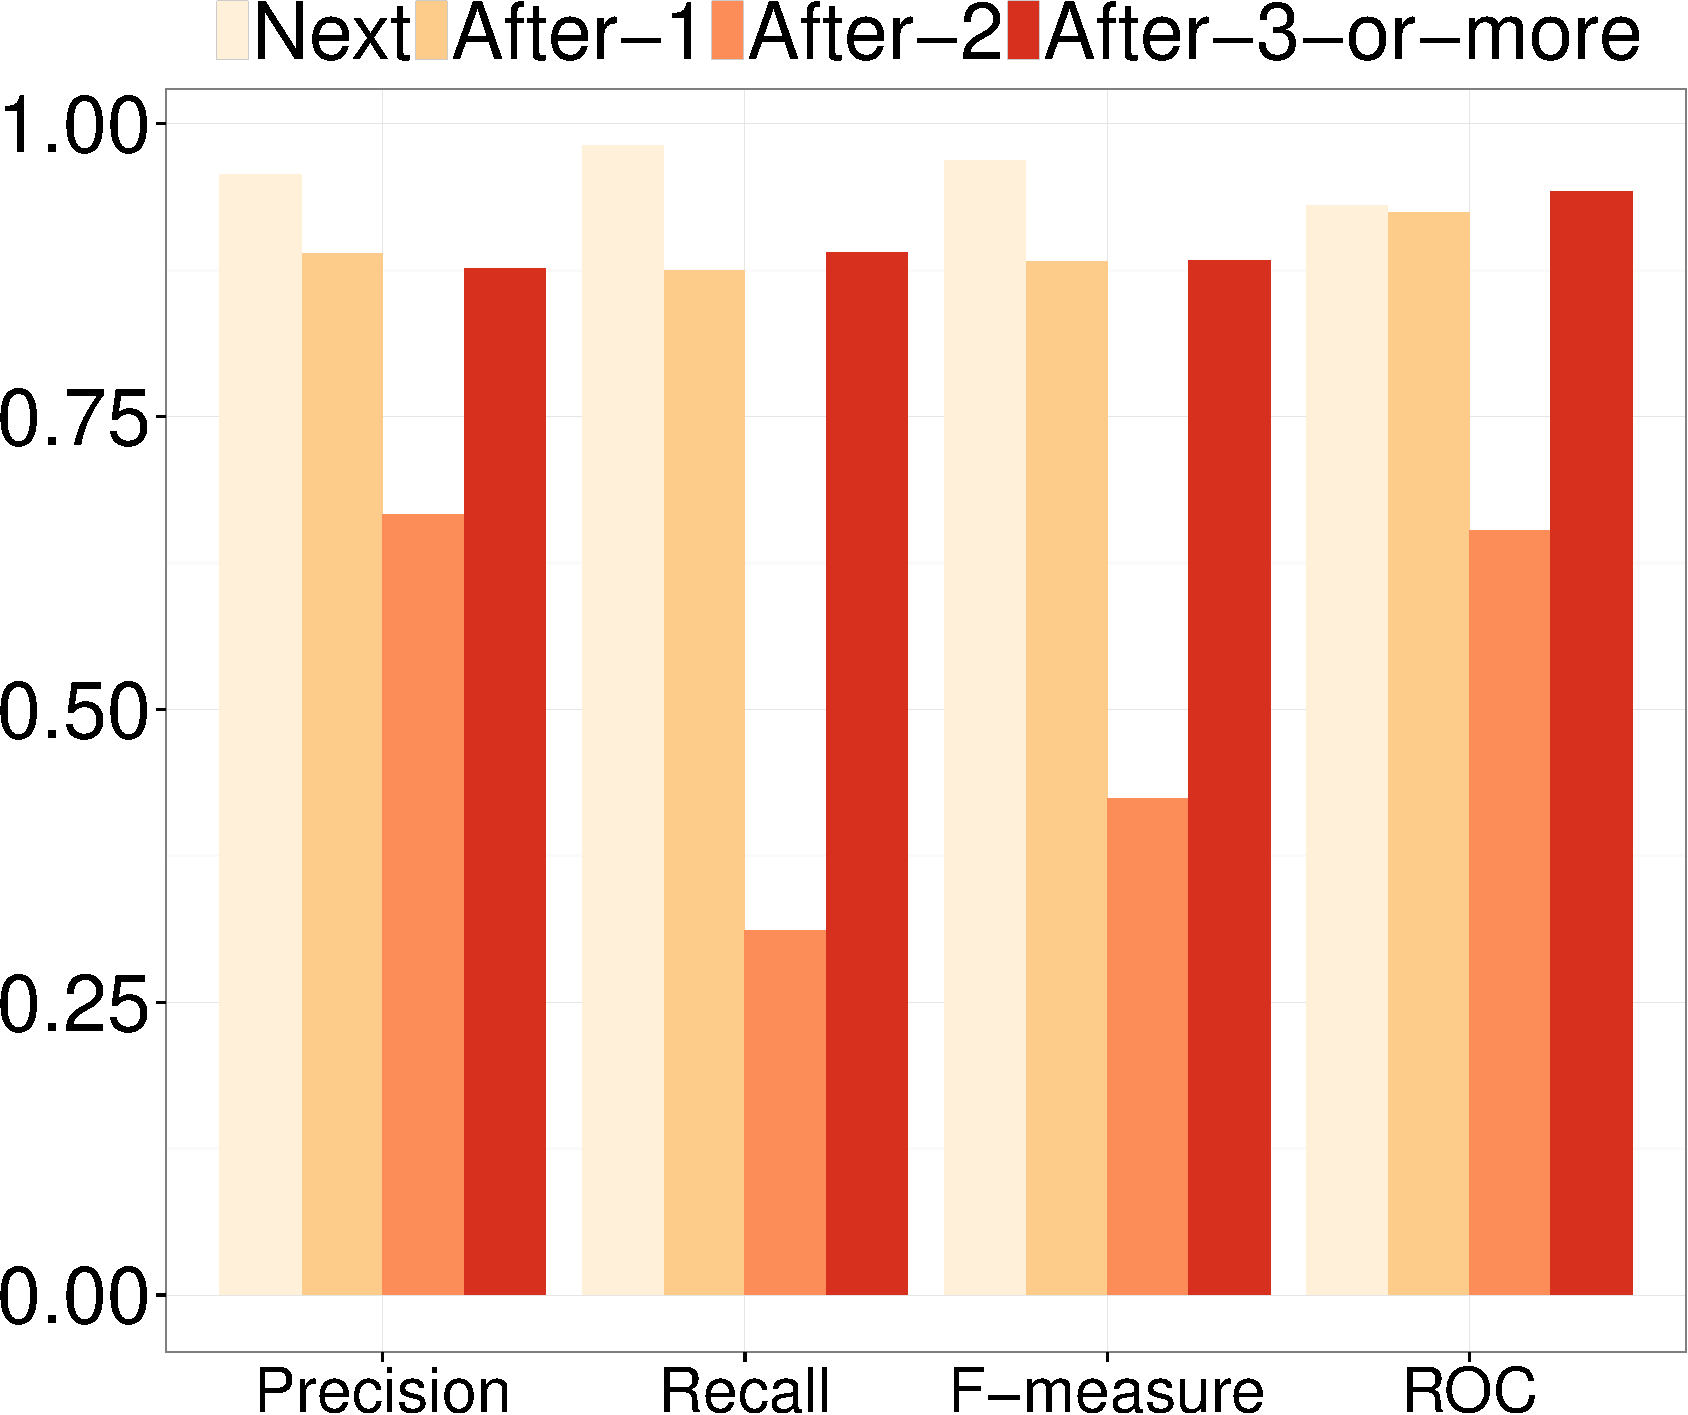
\includegraphics[width=0.50\textwidth,keepaspectratio] 
		{chapters/chapter4/figures/argouml_loocv_evaluation.pdf}
		\label{ch4:fig:RFargo}
	}
	\caption{\textbf{Performance of random forest models.} We show the
	values of Precision, Recall, F-measure, and AUC that are
computed using the LOOCV technique.}
	\label{ch4:fig:RFclassificationResult}
\end{figure}

\begin{table}
	\footnotesize
	\centering
	\caption{The precision, recall, F-measure, and AUC values that are
	obtained for the Eclipse, Firefox, and ArgoUML projects. 
	\label{ch4:tbl:evaluation_metrics}
	}
	\begin{tabular}{lcccc}
		\hline
		\multicolumn{5}{c}{\textbf{Eclipse}}\tabularnewline
		\hline 
		\textbf{Bucket} & \textbf{Precision} & \textbf{Recall} &
		\textbf{F-measure} & \textbf{AUC}\tabularnewline
		\hline 
		Next & 0.95  & 0.71  & 0.81 & 0.84 \tabularnewline
		\hline 
		After-1 & 0.75 & 0.89 & 0.81 & 0.88\tabularnewline
		\hline 
		After-2 & 0.82 & 0.95 & 0.88 & 0.94\tabularnewline
		\hline 
		After-3-or-more & 0.80 & 0.98 & 0.88 & 0.98\tabularnewline
		\hline 
		\hline
		\multicolumn{5}{c}{\textbf{Firefox}}\tabularnewline
		\hline 
		\textbf{Bucket} & \textbf{Precision} & \textbf{Recall} &
		\textbf{F-measure} & \textbf{AUC}\tabularnewline
		\hline 
		Next & 0.99  & 0.26  & 0.41 & 0.63 \tabularnewline
		\hline 
		After-1 & 0.74 & 0.17 & 0.28 & 0.58\tabularnewline
		\hline 
		After-2 & 0.92 & 0.99 & 0.96 & 0.61\tabularnewline
		\hline 
		After-3-or-more & 0.81 & 0.32 & 0.45 & 0.66\tabularnewline
		\hline 
		\hline
		\multicolumn{5}{c}{\textbf{ArgoUML}}\tabularnewline
		\hline 
		\textbf{Bucket} & \textbf{Precision} & \textbf{Recall} &
		\textbf{F-measure} & \textbf{AUC}\tabularnewline
		\hline 
		Next & 0.96  & 0.98  & 0.97 & 0.93 \tabularnewline
		\hline 
		After-1 & 0.89 & 0.87 & 0.88 & 0.92\tabularnewline
		\hline 
		After-2 & 0.67 & 0.31 & 0.42 & 0.65\tabularnewline
		\hline 
		After-3-or-more & 0.88 & 0.89 & 0.88 & 0.94\tabularnewline
		\hline 
	\end{tabular}
\end{table}

The best precision/recall values that we obtain for the Eclipse, Firefox, and
ArgoUML projects are related to the \textit{after-2} (F-measure of 0.88),
\textit{after-2} (F-measure of 0.96), and \textit{next} (F-measure of 0.97),
respectively. However, for buckets with low number of instances,
precision/recall values decrease considerably. For instance, the F-measures that
are obtained by our models for the Firefox project are considerably low for the
\textit{next}, \textit{after-1}, and \textit{after-3-or-more} buckets (0.41,
0.28 and 0.45, respectively).

Moreover, our models obtain median AUCs between 0.62 to 0.96, which indicate
that our model estimations are better than random guessing (AUC of 0.5).
Summarizing the results, our models obtain a median precision of 0.81-0.88
(median) and a median recall of 0.29-0.92. Our models provide a sound starting
point for studying the release into which an addressed issue will be delivered.\\

\noindent\finding{Our models obtain better F-measure values than
Zero-R.}{find7} We compared our models to Zero-R models as a baseline. For all test
instances, Zero-R selects the bucket that contains the majority of the instances.
Hence, the recall for the bucket containing the majority of instances is 1.0. We
compared the F-measure of our models to the F-measure of Zero-R models. We
choose to compare to the F-measure values because precision and recall are very
skewed for Zero-R. 

For the Firefox project, Zero-R obtains an F-measure of 0.95 for the
\textit{after-2} bucket, whereas our model obtains an F-measure of 0.96 for the
same bucket. For the Eclipse project, Zero-R always selects \textit{next} and
obtains a F-measure of 0.58, while our model obtains an F-measure of 0.81.
Finally, for the ArgoUML project, Zero-R always selects \textit{next} with an
F-measure of 0.84, whereas our model obtains an F-measure of 0.97. These results
show that our models yield better F-measure values than na\"{i}ve techniques
like Zero-R or random guessing (AUC = 0.5) in the majority of cases.  

\conclusionbox{We are able to accurately model how many releases an addressed issue
is likely to be prevented from delivery. Our models outperform na\"{i}ve
techniques, such as Zero-R and random guessing, obtaining AUC values of 0.62 to
0.96.}

\begin{table}
	\centering
	\footnotesize
	\caption{\textbf{Regression results of model fit.} Our explanatory
		models obtain $R^2$ values between 0.39 to 0.65 and MAE values between
	7.8 to 66 days.}
	\label{ch4:tbl:regression_results}
	\def\arraystretch{1.5}
	\begin{tabular}{lrrr}
		\hline 
		\centering{\textbf{Metric/Project}} &
		\centering{\textbf{Eclipse}} & \centering{\textbf{Firefox}} &
		\centering{\textbf{ArgoUML}} \tabularnewline
		\hline 
		$R^2$ & 0.48  & 0.39 & 0.65 \tabularnewline
		\hline 
		MAE (days) & 61 & 7.8  & 66 \tabularnewline
		\hline 
		Release cycle duration (median in days) & 112 & 42 & 180 \tabularnewline
		\hline
		Error ratio $(\frac{MAE}{cycle})$ & 0.54  & 0.18  & 0.37 \tabularnewline
		\hline 
		Optimism & 0.0267 & 0.0162 & 0.0035 \tabularnewline
		\hline 
	\end{tabular}
\end{table}

\subsubsection*{\textit{\textbf{RQ3: Results for delivery delay in terms of days}}}

\noindent\finding{Our explanatory models obtain $R^2$ values of 0.39-0.65
and MAE values between 7.8 to 67 days.}{find8} Our models obtain fair $R^2$ values to
model the variability of delivery delay in days in the studied projects.
\hyperref[ch4:tbl:regression_results]{Table}~\ref{ch4:tbl:regression_results} shows the
$R^2$ and MAE values that are obtained by each of our regression models. The
$R^2$ values for the Eclipse, Firefox, and ArgoUML projects are of 0.39, 0.48,
and 0.65, respectively. 
Additionally, our regression models can provide fair
estimations of delivery delay in days, specially for the Firefox project. For
instance, the median interval in days between releases of the Firefox project is
42 days
(see~\hyperref[ch4:fig:releaseIntervals]{Figure}~\ref{ch4:fig:releaseIntervals}), while
the MAE value for the Firefox project is 7.8 days, which equates to an error
ratio of 18\% (see
\hyperref[ch4:tbl:regression_results]{Table}~\ref{ch4:tbl:regression_results}).\\

\noindent\finding{Our explanatory models obtain a good stability with bootstrap
calculated optimism between 0.0035 to 0.0267 of the $R^2$ values.}{find9} We also
observe that our regression models are stable.
\hyperref[ch4:tbl:regression_results]{Table}~\ref{ch4:tbl:regression_results} shows the
\textit{bootstrap-calculated} optimism of the $R^2$ values of our models. The
optimism for the Eclipse, Firefox and ArgoUML projects are 0.0267, 0.0162, and 0.0035,
respectively. Such results indicate that our explanatory models are unlikely to
be overfitted to our data and that our models are stable enough for us to perform the
statistical inferences that follow. 

\conclusionbox{We are able to accurately estimate the delivery delay in terms
of number of days. Our models obtain fair $R^2$ values of 0.39 to 0.65. Our
exploratory models are quite stable with a maximum optimism of 0.0267.}

\subsection{RQ4: What are the most influential attributes for
modeling delivery delay?}\label{ch4:rq4}

\subsubsection*{RQ4: Motivation} In \hyperref[ch4:rq3]{RQ3}, we found that our
models can accurately model the delivery delay of addressed issues. To fit our
models, we use attributes that we collect from ITSs and VCSs. As described in
\hyperref[ch4:tbl:dimensions]{Tables}~\ref{ch4:tbl:dimensions},~\ref{ch4:tbl:dimensions2}
and~\ref{ch4:tbl:dimensions3}, the attributes belong to different families that
are related to addressed issues. In \hyperref[ch4:rq4]{RQ4}, we investigate
which attributes are influential to estimate the delivery delay of addressed
issues. We present the approaches and results of \hyperref[ch4:rq4]{RQ4} for
each studied type of delivery delay (\hyperref[def:1]{Definitions}~\ref{def:1}
and~\ref{def:2}). 

\subsubsection*{RQ4: Approach}

To identify the most influential attributes for estimating the delivery delay
in terms of releases (\hyperref[def:1]{Definition}~\ref{def:1}), we compute the
\textit{variable importance} score for each attribute of our models. The
\textit{variable importance} implementation that we use in our study is
available within the \textit{bigrf} R package. This implementation computes the
importance score based on {\em Out Of the Bag} (OOB) estimates. Each attribute
of the dataset is randomly permuted in the OOB data.  Then, the average \(a\) of
the differences between the votes for the correct bucket in the permuted OOB and
the original OOB is computed. The result of \(a\) is the importance of an
attribute. 

The final output of the variable importance is a rank of the attributes
indicating their importance for the model. Hence, if a specific attribute has
the highest rank, then it is the most influential attribute that our explanatory
model is using to estimate delivery delay. Finally, we use the models with the
largest training corpus when performing the LOOCV to compute the variable
importance scores.

We perform Step~6.2 of
\hyperref[ch4:fig:regression_process]{Figure}~\ref{ch4:fig:regression_process} to
identify the most influential attributes in our models that we fit to study the
delivery delay in terms of number of days
(\hyperref[def:2]{Definition}~\ref{def:2}). We evaluate the explanatory power of
each attribute by using the Wald $\chi^2$ maximum likelihood test (Step~6.2).
The larger the $\chi^2$ value, the greater the power that a particular attribute
has to model the variability of delivery delay in terms of days. To do so, we
use the \code{anova} function of the \code{rms} R package.

\subsubsection*{\textit{\textbf{RQ4: Results for delivery delay in terms of
releases}}}

\noindent\finding{The fixing time per resolver and integration workload
attributes are the most influential attributes in our models.}{find10}
\hyperref[ch4:fig:variableImportance]{Figure}~\ref{ch4:fig:variableImportance} shows the
variable importance values of the LOOCV of our models. The most influential
attribute is the \textit{fixing time per resolver}. The \textit{fixing time per
resolver} attribute measures the total time that is spent by each resolver on
fixing issues in a release cycle. The second most influential attributes are
integration workload attributes (\ie backlog of issues and backlog of issues per
resolver). These integration workload attributes measure the competition of
issues that were addressed but not yet delivered through an official release.

\begin{figure}
	\center
	\subfloat[Eclipse]{
		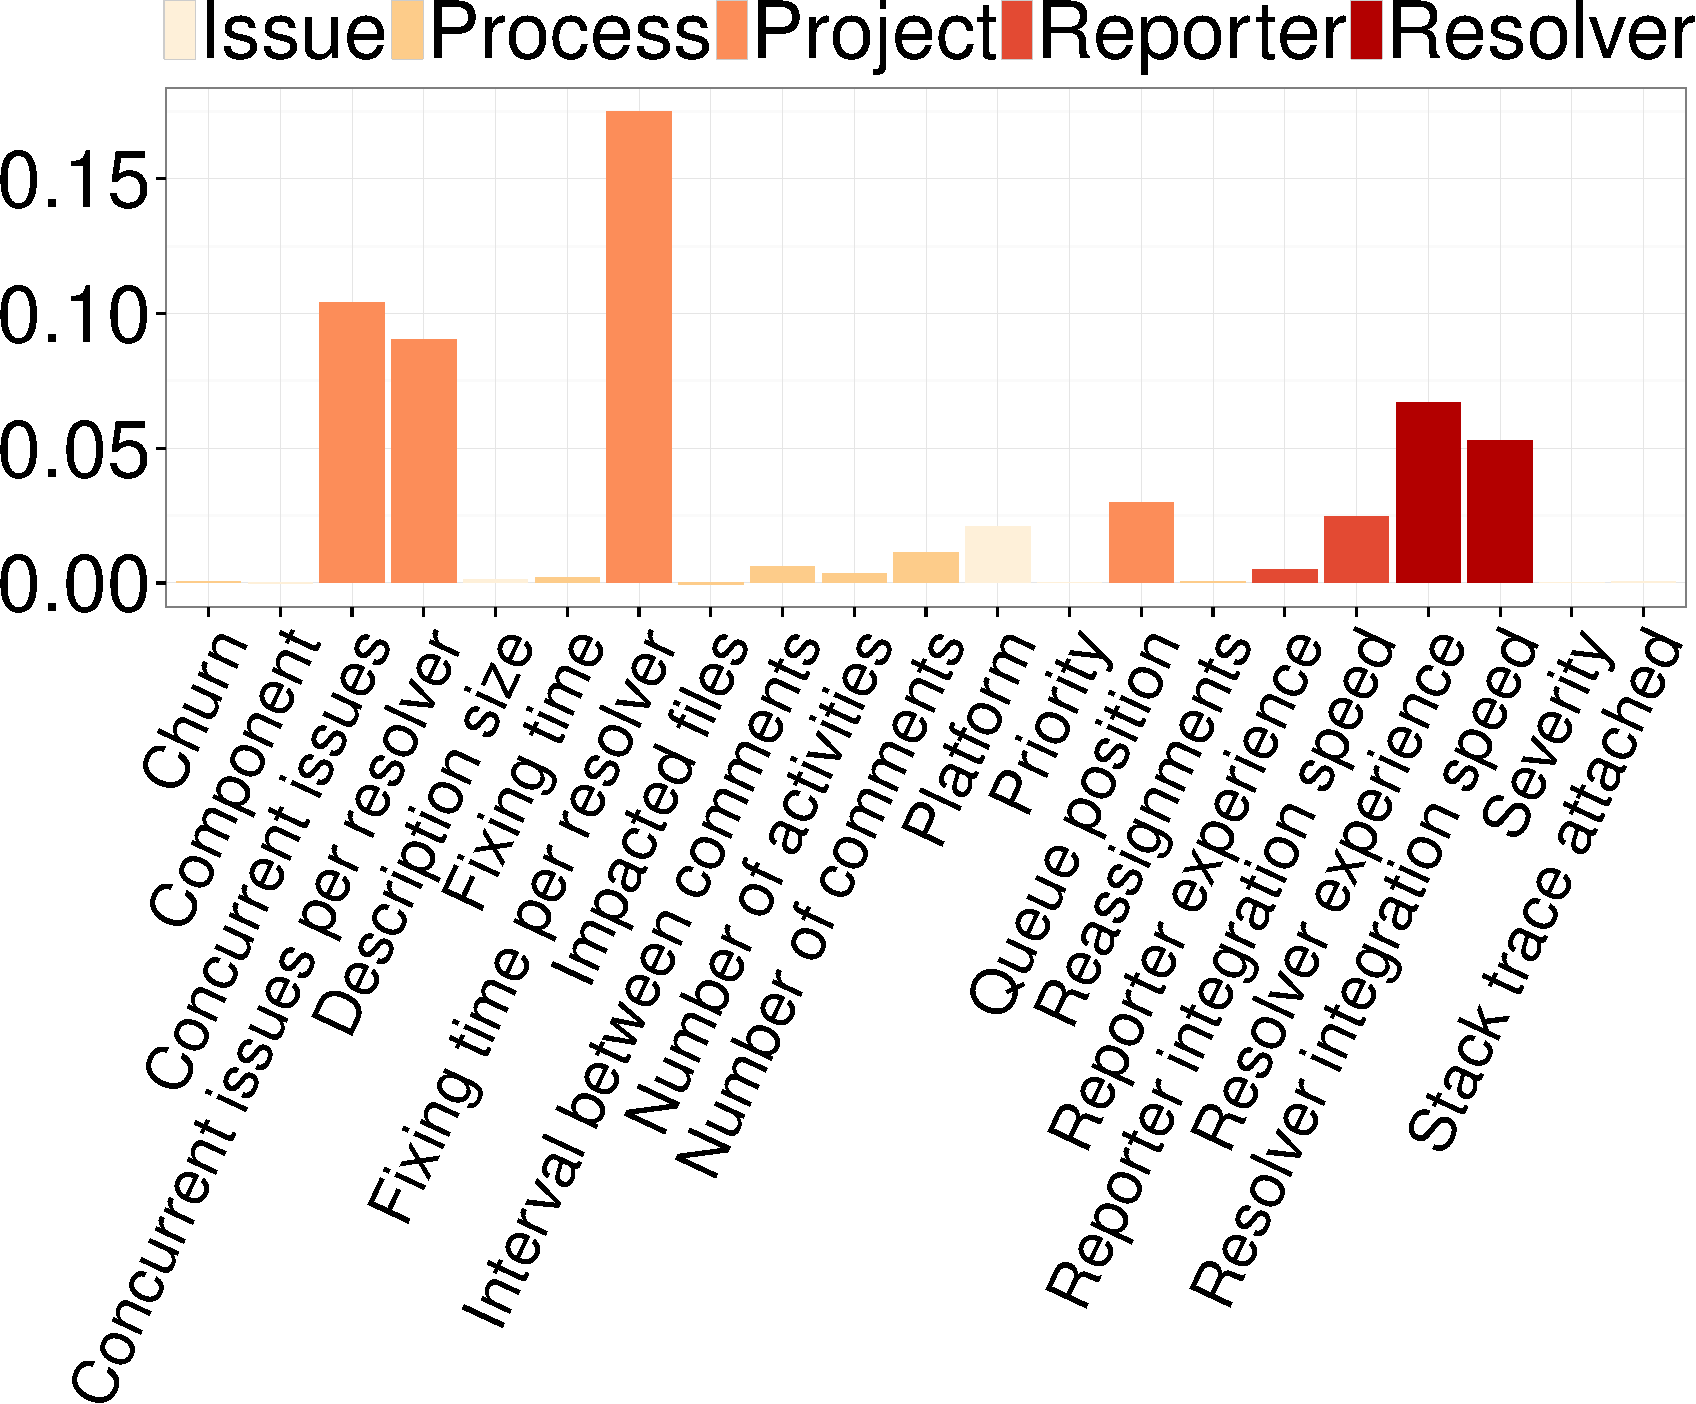
\includegraphics[width=0.55\textwidth,keepaspectratio] 
		{chapters/chapter4/figures/eclipse_loocv_varimp.pdf}
	\label{ch4:fig:impEclipse}
	}

	\subfloat[Firefox]{
		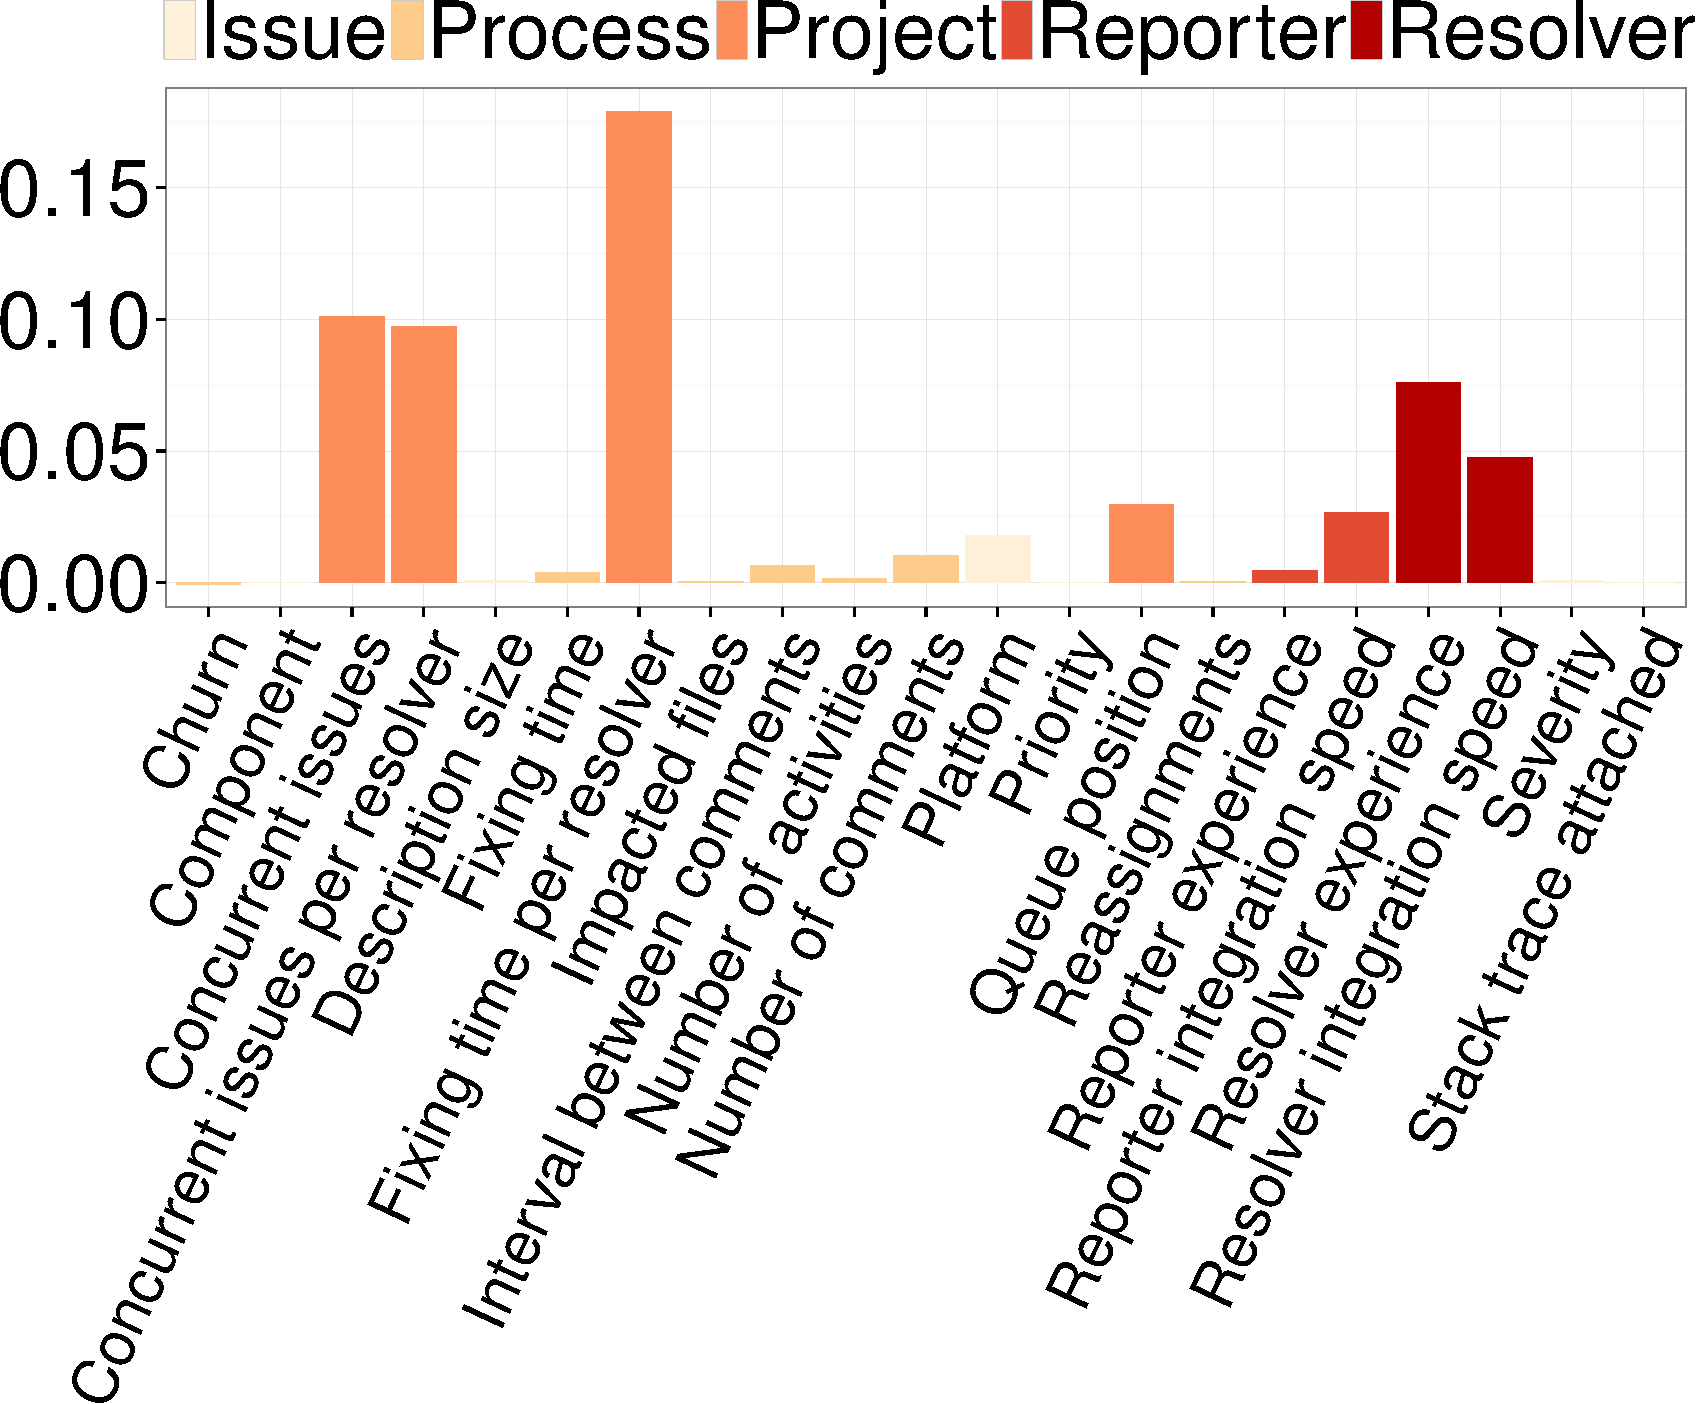
\includegraphics[width=0.55\textwidth,keepaspectratio]  
		{chapters/chapter4/figures/firefox_loocv_varimp.pdf}
		\label{ch4:fig:impFirefox}
	}

	\subfloat[ArgoUML]{
		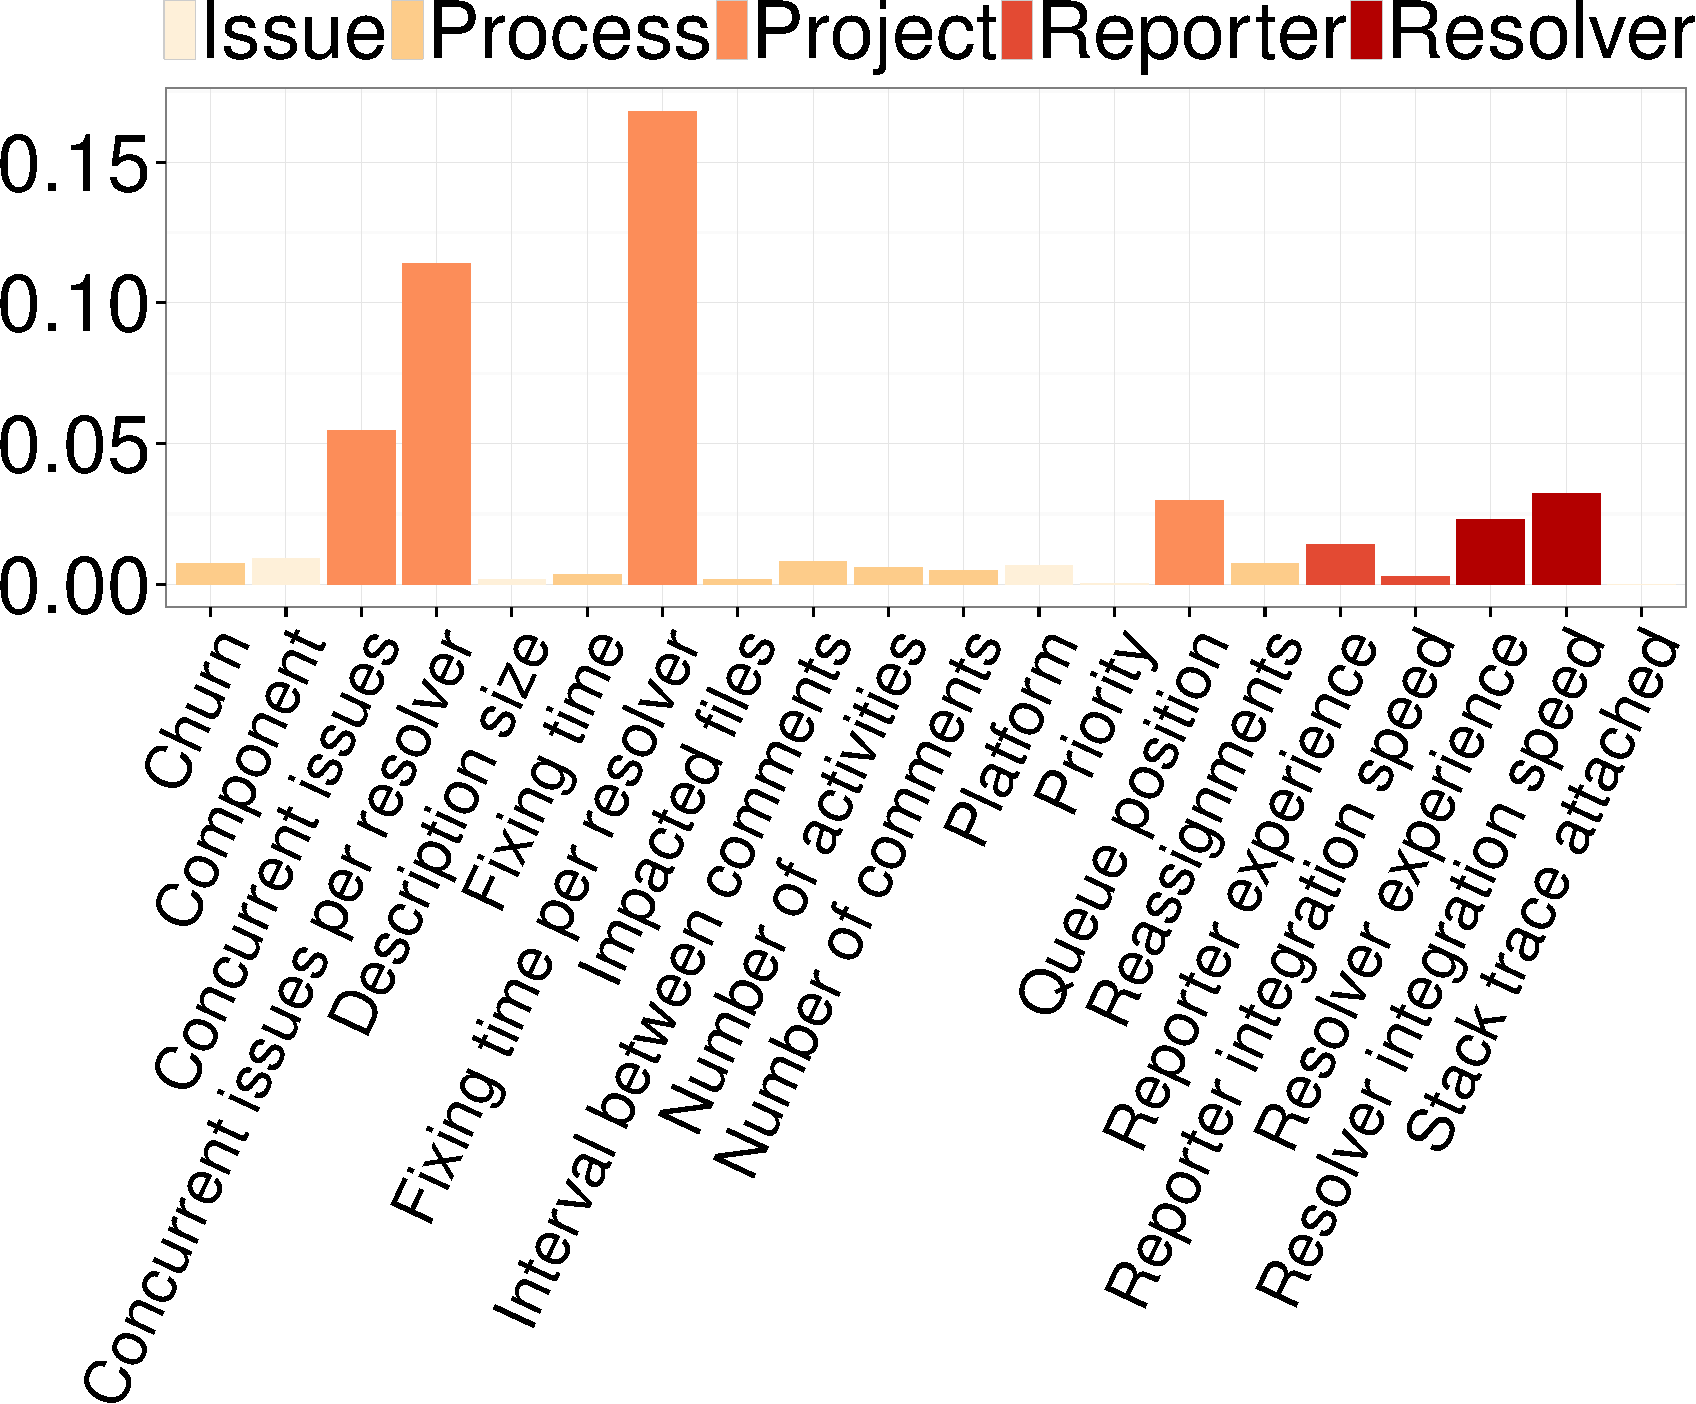
\includegraphics[width=0.55\textwidth,keepaspectratio] 
		{chapters/chapter4/figures/argouml_loocv_varimp.pdf}
	\label{ch4:fig:impArgo}}
	\caption{\textbf{Variable importance scores.} We show the 
		importance scores that are computed for the LOOCV of our models.}
	\label{ch4:fig:variableImportance}
\end{figure}

Our results suggest that the time that is invested by the resolvers on fixing
issues have a strong association with delivery delay. This could be due to
resolvers fixing issues more carefully---which would lead to a smoother
delivery of such issues---or issues that were less complex in overall (\eg a
shorter time was invested), which might simplify the delivery process. A deeper
analysis of this attribute would be necessary to better understand the exact
reasons behind this relationship (\eg consulting the development team through
surveys and interviews). 

We also observe that integration workload attributes (\ie \textit{backlog of
issues} and \textit{backlog of issues per resolver}) are the second most
influential attributes in the three studied projects. This finding suggests that
the integration backlog introduces overhead that may lead to longer delivery
delay.

\begin{figure}[!t]
	\centering
	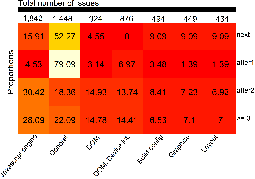
\includegraphics[width=0.60\textwidth,keepaspectratio]
	{chapters/chapter4/figures/firefox/RQ3_component_hm.pdf}
	\caption{\textbf{The spread of issues among the Firefox components.} The
		darker the colors, the smaller the proportion of issues that
	impact that component.}
	\label{ch4:fig:componentHeatmap}
\end{figure}

Furthermore, we study the distribution of addressed issues across components in the
Firefox project.
\hyperref[ch4:fig:componentHeatmap]{Figure}~\ref{ch4:fig:componentHeatmap} shows the top
seven components of the Firefox project, each having more than 400 addressed issues.
We analyze the proportion of addressed issues where delivery was prevented in the
top seven components.
\hyperref[ch4:fig:componentHeatmap]{Figure}~\ref{ch4:fig:componentHeatmap} shows that,
for buckets \textit{next} and \textit{after-1}, the majority of issues are
related to the \textit{General component}, whereas for \textit{after-2} and
\textit{after-3-or-more} the majority are related to the \textit{Javascript
engine} component. Addressed issues related to the \textit{General} component
may be easy to integrate, whereas issues related to the \textit{Javascript
Engine} may require more careful analysis before delivery.  \\


\noindent\finding{Severity and priority have little influence on
delivery delay in terms of releases.}{find11} Users and contributors of software
projects can denote the importance of an issue using the \textit{priority} and
\textit{severity} fields. Previous studies have shown that priority and
severity have little influence on bug fixing time
\cite{tian2015unreliability,Herraiz2008,Mockus:2002}. For example, while an
issue might be severe or of high priority, it might be complex and would take a
long time to fix.  

However, in the integration context, we expect that priority and severity would
be more influential, since the issues have already been addressed. Even though
priority and severity are often left at their default values (see
\hyperref[ch4:sec:subjects]{Section}~\ref{ch4:sec:subjects}), one would expect that the
integrators would fast-track the integration of issues for which they
care about increasing the levels of severity or priority. For instance,
according to the Eclipse project guidelines for filing issue reports, a priority
level of P1 is used for serious issues and specifies that the existence of a P1
issue should prevent a release from
shipping.\smartfoot{\url{http://wiki.eclipse.org/Development_Resources/HOWTO/Bugzilla_Use}}
Hence, it is surprising that priority and severity play such a small role in
determining the release in which an addressed issue will appear. Indeed,
\hyperref[ch4:fig:variableImportance]{Figure}~\ref{ch4:fig:variableImportance} shows
that the priority and severity metrics obtain low importance scores.

\begin{figure}
	\centering
	%\captionsetup{justification=centering}
	\subfloat[ArgoUML Priority]{
		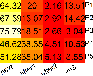
\includegraphics[width=0.30\textwidth,keepaspectratio] 
		{chapters/chapter4/figures/argouml/RQ3_priority_hm.pdf}
	\label{ch4:fig:heatMap_argo}}
	\subfloat[Eclipse Priority]{
		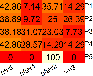
\includegraphics[width=0.30\textwidth,keepaspectratio] 
		{chapters/chapter4/figures/eclipse/RQ3_priority_hm.pdf}
	\label{ch4:fig:heatMap_eclipsep}}
	\subfloat[Firefox Priority]{
		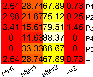
\includegraphics[width=0.30\textwidth,keepaspectratio]  
		{chapters/chapter4/figures/firefox/RQ3_priority_hm.pdf}
		\label{ch4:fig:heatMap_firefoxp}
	}

	\subfloat[Eclipse Severity]{
		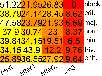
\includegraphics[width=0.35\textwidth,keepaspectratio] 
		{chapters/chapter4/figures/eclipse/RQ3_severity_hm.pdf}
	\label{ch4:fig:heatMap_eclipses}}
	\subfloat[Firefox Severity]{
		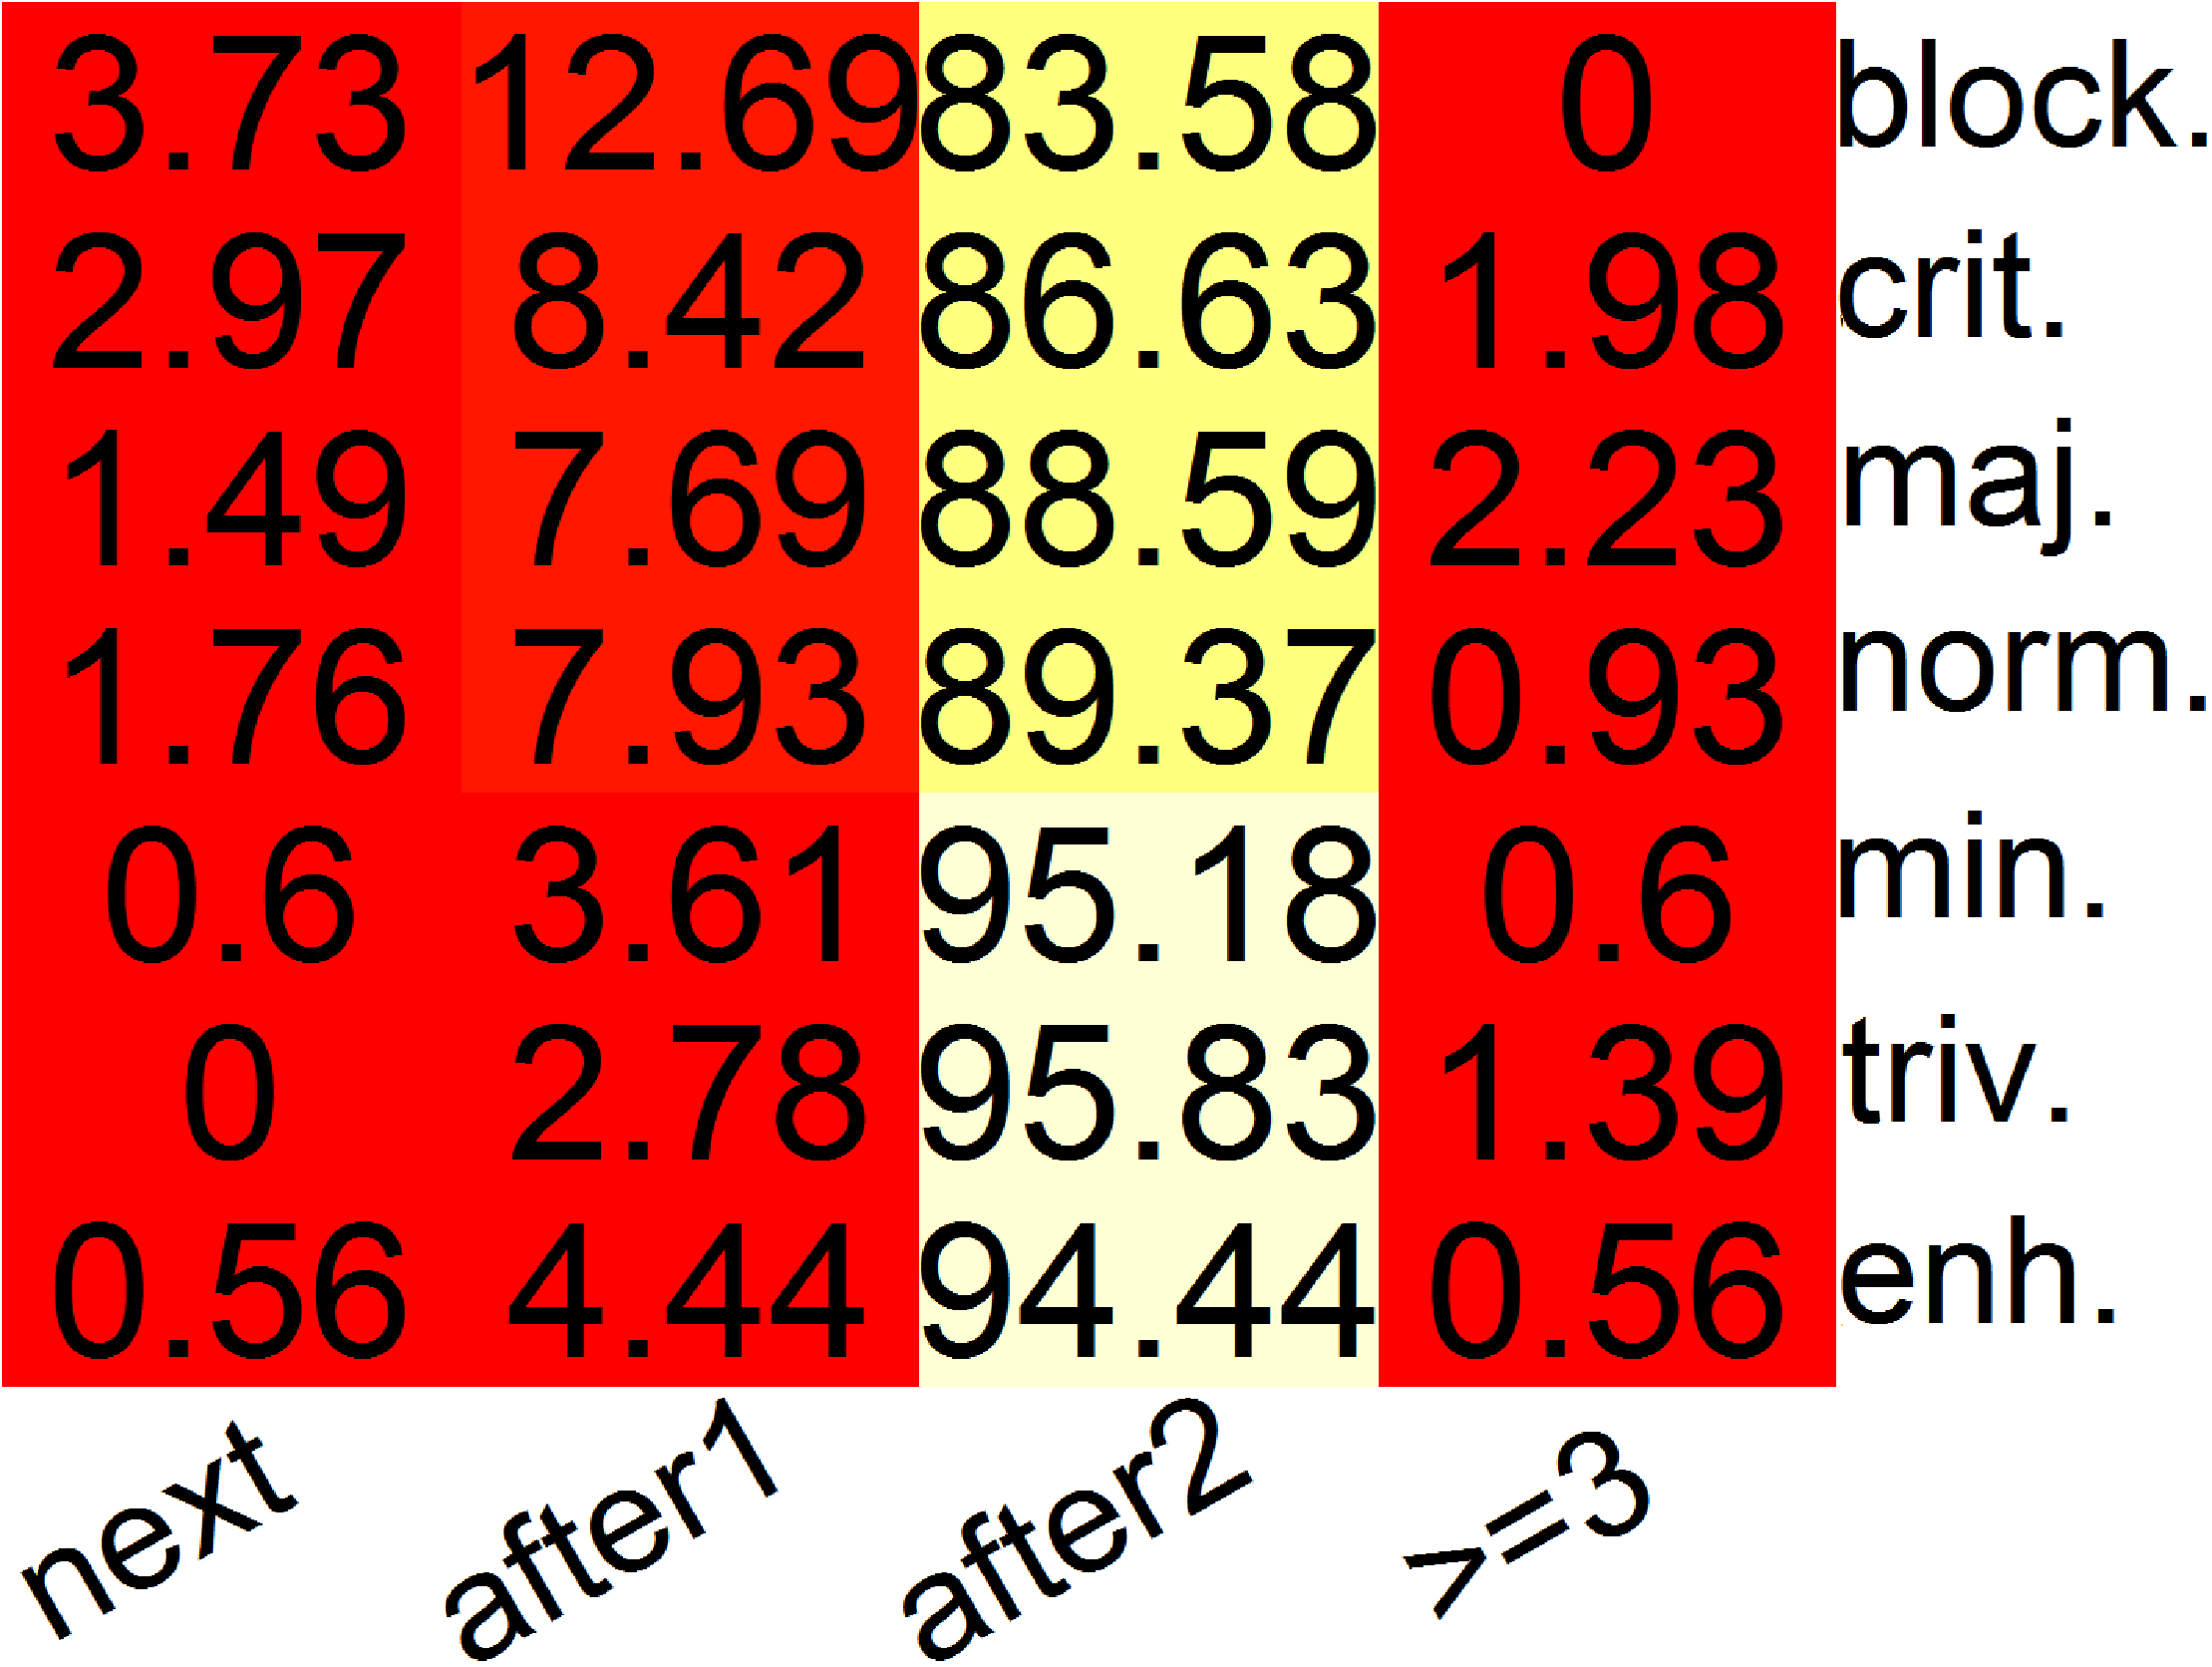
\includegraphics[width=0.35\textwidth,keepaspectratio]  
		{chapters/chapter4/figures/firefox/RQ3_severity_hm.pdf}
		\label{ch4:fig:heatMap_firefoxs}
	}
	\caption{\textbf{The percentage of priority and severity levels in each
		studied bucket of delivery delay.} We expect to see light
		colour in the upper left corner of these graphs, indicating that
		high priority/severity issues are delivered quickly.
	Surprisingly, we are not seeing such a pattern in our datasets.}
	\label{ch4:fig:heatMaps}
\end{figure}

\hyperref[ch4:fig:heatMaps]{Figure}~\ref{ch4:fig:heatMaps} shows the percentage of
issues with a given priority (\textit{y-axis}) in a given delivery delay bucket
(\textit{x-axis}). The delivery of 36\% to 97\% of priority P1 addressed issues
had their delivery prevented in at least one release, whereas the delivery
of 32\% to 96\% of priority P2 addressed issues were prevented from delivery in
at least one release. 

In the ArgoUML project, while the majority of priority P1 issues (64\%) were
delivered in the \textit{next} release, 36\% of them had their delivery
prevented in at least one release. For the Firefox project, 97\% of the P1
issues and 96\% of the \textit{blocker} issues were prevented from delivery
in at least one release. Finally, for the Eclipse project, 57\% of P1 issues and
49\% of blocker issues had their delivery prevented in at least one release.
Hence, our data shows that, in the context of issue delivery, the
\textit{priority} and \textit{severity} values that are recorded in the ITSs
have little influence on delivery delay. Instead, addressed issues might be
prioritized by the level of risk that are associated to them.\smartfoot{Two
	issues from our sample were promoted to stabler release channels due to
	low associated risk
	\url{https://bugzilla.mozilla.org/show_bug.cgi?id=724145} and
	\url{https://bugzilla.mozilla.org/show_bug.cgi?id=732962}, while another
	issue was prevented from delivery due to code break
\url{https://bugzilla.mozilla.org/show_bug.cgi?id=723793}.} This might explain
why the time that is invested on fixing issues during a release cycle reduces
delivery delay---a risk of an addressed issue breaking the code would be smaller
when more time is invested at fixing activities. 

\conclusionbox{The total time that is invested in fixing issues of a release
	cycle and integration workload attributes are the most influential
	attributes in our models. We also find that priority and severity have
	little influence in estimating delivery delay.}

\subsubsection*{\textbf{\textit{RQ4: Results for delivery delay in terms of days}}}

\begin{table}[t]
	\scriptsize
	\centering
	\caption{\textbf{Explanatory power of attributes.} We present the
		$\chi^2$ proportion and the degrees of freedom that are spent
		for each attribute. The $\chi^2$ of the two most influential
		attributes of each model are in bold.
	\label{ch4:tbl:explanatory_power}}
	\begin{threeparttable}
		\begin{tabular}{llrrr}
			\cline{3-5} 
			\multicolumn{2}{c}{} & 
			Eclipse &
			Firefox &
			ArgoUML
			\tabularnewline
			\hline
			\multicolumn{2}{l}{Wald $\chi^2$} & 
			$1,180$ &
			$8,560$ &
			$2,803$
			\tabularnewline
			\hline 
			\multicolumn{2}{l}{Budgeted Degrees of Freedom} &
			$87$ & 
			$879$ &
			$102$
			\tabularnewline
			\hline
			\multicolumn{2}{l}{Degrees of Freedom Spent} &
			$24$ & 
			$33$ &
			$28$
			\tabularnewline
			\hline 
			\multirow{2}{*}{Reporter experience} & 
			D.F. & 
			$1$ & 
			$1$ &
			$1$
			\tabularnewline 
			& 
			$\chi^2$ & 
			$4^{\ast\ast\ast}$ &  
			$\approx 0$ &
			$1^{\ast\ast}$
			\tabularnewline
			\hline 
			\multirow{2}{*}{Resolver experience} & 
			D.F. & 
			$1$ & 
			$1$ &
			$1$
			\tabularnewline 
			& 
			$\chi^2$ & 
			$12^{\ast\ast\ast}$ & 
			$\approx 0^{\ast}$ &  
			$\approx 0$ 
			\tabularnewline
			\hline 
			\multirow{2}{*}{Reporter integration speed} & 
			D.F. & 
			$3$ & 
			$1$ &
			$2$
			\tabularnewline &
			$\chi^2$ & 
			$16^{\ast\ast\ast}$ &
			$\approx 0$ &
			$1^{\ast}$
			\tabularnewline  
			\hline 
			\multirow{2}{*}{Resolver integration speed} & 
			D.F. & 
			$2$ & 
			$1$ &
			$4$
			\tabularnewline & 
			$\chi^2$ & 
			$\mathbf{22}^{\ast\ast\ast}$ &
			$\approx 0$ &  
			$\mathbf{9}^{\ast\ast\ast}$
			\tabularnewline
			\hline 
			\multirow{2}{*}{Fixing time} & 
			D.F. & 
			$2$ & 
			\multirow{2}{*}{$\oplus$} &
			$1$
			\tabularnewline & 
			$\chi^2$ & 
			$1^{\ast}$ &
			&  
			$1^{\ast\ast}$ 
			\tabularnewline
			\hline 
			\multirow{2}{*}{Severity} & 
			D.F. & 
			$6$ &
			$6$ &
			\multirow{2}{*}{$\ominus$} 
			\tabularnewline & 
			$\chi^2$ &
			$\approx 0$ &
			$8^{\ast\ast\ast}$ &
			%\ominus
			\tabularnewline \hline 
			\multirow{2}{*}{Priority} &
			D.F. & 
			\multirow{2}{*}{$\oslash$} & 
			$5$ &
			$5$
			\tabularnewline & 
			$\chi^2$ & 
			&%\oslash
			$5^{\ast\ast\ast}$ &  
			$1^{\ast}$  
			\tabularnewline \hline 
			\multirow{2}{*}{Description size} & 
			D.F. & 
			$1$ & 
			$1$ &
			$1$
			\tabularnewline & 
			$\chi^2$ & 
			$\approx 0$ &  
			$\approx 0$ &
			$\approx 0$
			\tabularnewline \hline 
			\multirow{2}{*}{Impacted files} & 
			D.F. & 
			$1$ &
			$1$ &
			$1$
			\tabularnewline & 
			$\chi^2$ & 
			$\approx 0$ &
			$\approx 0^{\ast\ast}$ &
			$\approx $
			\tabularnewline \hline 
			\multirow{2}{*}{Number of comments} & 
			D.F. & 
			$1$ &
			$1$ &  
			$1$
			\tabularnewline & 
			$\chi^2$ & 
			$2^{\ast\ast}$ &  
			$1^{\ast\ast\ast}$  &
			$\approx 0$
			\tabularnewline \hline 
			\multirow{2}{*}{Reassignments} & 
			D.F. & 
			$1$ & 
			$1$ &
			$1$
			\tabularnewline & 
			$\chi^2$ & 
			$\approx 0$ &  
			$\approx 0$ &
			$1^{\ast}$
			\tabularnewline \hline 
			\multirow{2}{*}{Number of activities} & 
			D.F. & 
			$1$ &
			$1$ &
			$1$
			\tabularnewline & 
			$\chi^2$ & 
			$\approx 0$ &  
			$\approx 0$ &
			$\approx 0$
			\tabularnewline \hline 
			\multirow{2}{*}{Interval between comments} & 
			D.F. & 
			$1$ &
			$1$ &
			\multirow{2}{*}{$\oslash$}
			\tabularnewline & 
			$\chi^2$ & 
			$1^{\ast}$ &  
			$\approx 0$ &
			%\oslash correlation
			\tabularnewline \hline 
			\multirow{2}{*}{Churn} & 
			D.F. & 
			$1$ &
			$1$ &
			$1$
			\tabularnewline & 
			$\chi^2$ & 
			$\approx 0$ &  
			$\approx 0$ &
			$1^{\ast\ast}$
			\tabularnewline \hline 
			\multirow{2}{*}{Number of concurrent issues} & 
			D.F. & 
			\multirow{2}{*}{$\oslash$} &
			$2$ &
			\multirow{2}{*}{$\oslash$}
			\tabularnewline &
			$\chi^2$ &
			& %\oslash
			$\mathbf{8}^{\ast\ast\ast}$ &
			%\oslash
			\tabularnewline \hline 
			\multirow{2}{*}{Number of concurrent issues per resolver} & 
			D.F. & 
			$1$ & 
			$2$ &
			$2$
			\tabularnewline &
			$\chi^2$ &
			$7^{\ast\ast\ast}$ &  
			$2^{\ast\ast\ast}$ &
			$\mathbf{9}^{\ast\ast\ast}$
			\tabularnewline \hline 
			\multirow{2}{*}{Queue position} & 
			D.F. & 
			$1$ &             
			$4$ &
			$2$
			\tabularnewline & 
			$\chi^2$ & 
			$\mathbf{23}^{\ast\ast\ast}$ & 
			$\mathbf{83}^{\ast\ast\ast}$ &
			$\mathbf{67}^{\ast\ast\ast}$
			\tabularnewline \hline 
			\multirow{1}{*}{Fixing time per resolver} & 
			D.F. & 
			$1$ & 
			$2$ &
			$4$
			\tabularnewline &
			$\chi^2$ & 
			$7^{\ast\ast\ast}$ & 
			$\approx 0^{\ast\ast}$ &
			$8^{\ast\ast\ast}$
			\tabularnewline \hline 
		\end{tabular}
		\begin{tablenotes}
		\item[$\oslash$] Discarded during correlation analysis 
		\item[$\oplus$] Discarded during redundancy analysis 
		\item[$\ominus$] The variable does not apply to the dataset
		\item[$\ast$] $p < 0.05$
		\item[$\ast\ast$] $p < 0.01$
		\item[$\ast\ast\ast$] $p < 0.001$ 
		\end{tablenotes}
	\end{threeparttable}
\end{table}

\noindent\finding{Project family attributes, such as the backlog of
issues and queue position provide most of the explanatory power of our
models.}{find12}
\hyperref[ch4:tbl:explanatory_power]{Table}~\ref{ch4:tbl:explanatory_power} shows the
explanatory power of each of the attributes of our models. The two most
influential attributes for each model are shown in bold. \textit{Queue
position}, \ie the time at which an issue is addressed is the most influential
attribute in all of the models that are fitted to our studied projects.
Interestingly, we observe that \textit{resolver integration speed}---the median
delivery delay of the previously resolved issues of a particular
resolver---plays an influential role in our models that are fit for the Eclipse
and ArgoUML projects. Moreover, we also observe that integration workload
attributes (\ie \textit{backlog of issues}, and \textit{backlog of issues per
resolver}) are very influential in our models that are fit for the Firefox and
ArgoUML projects.\\

\begin{figure}
	\centering
	\subfloat[Eclipse]{
		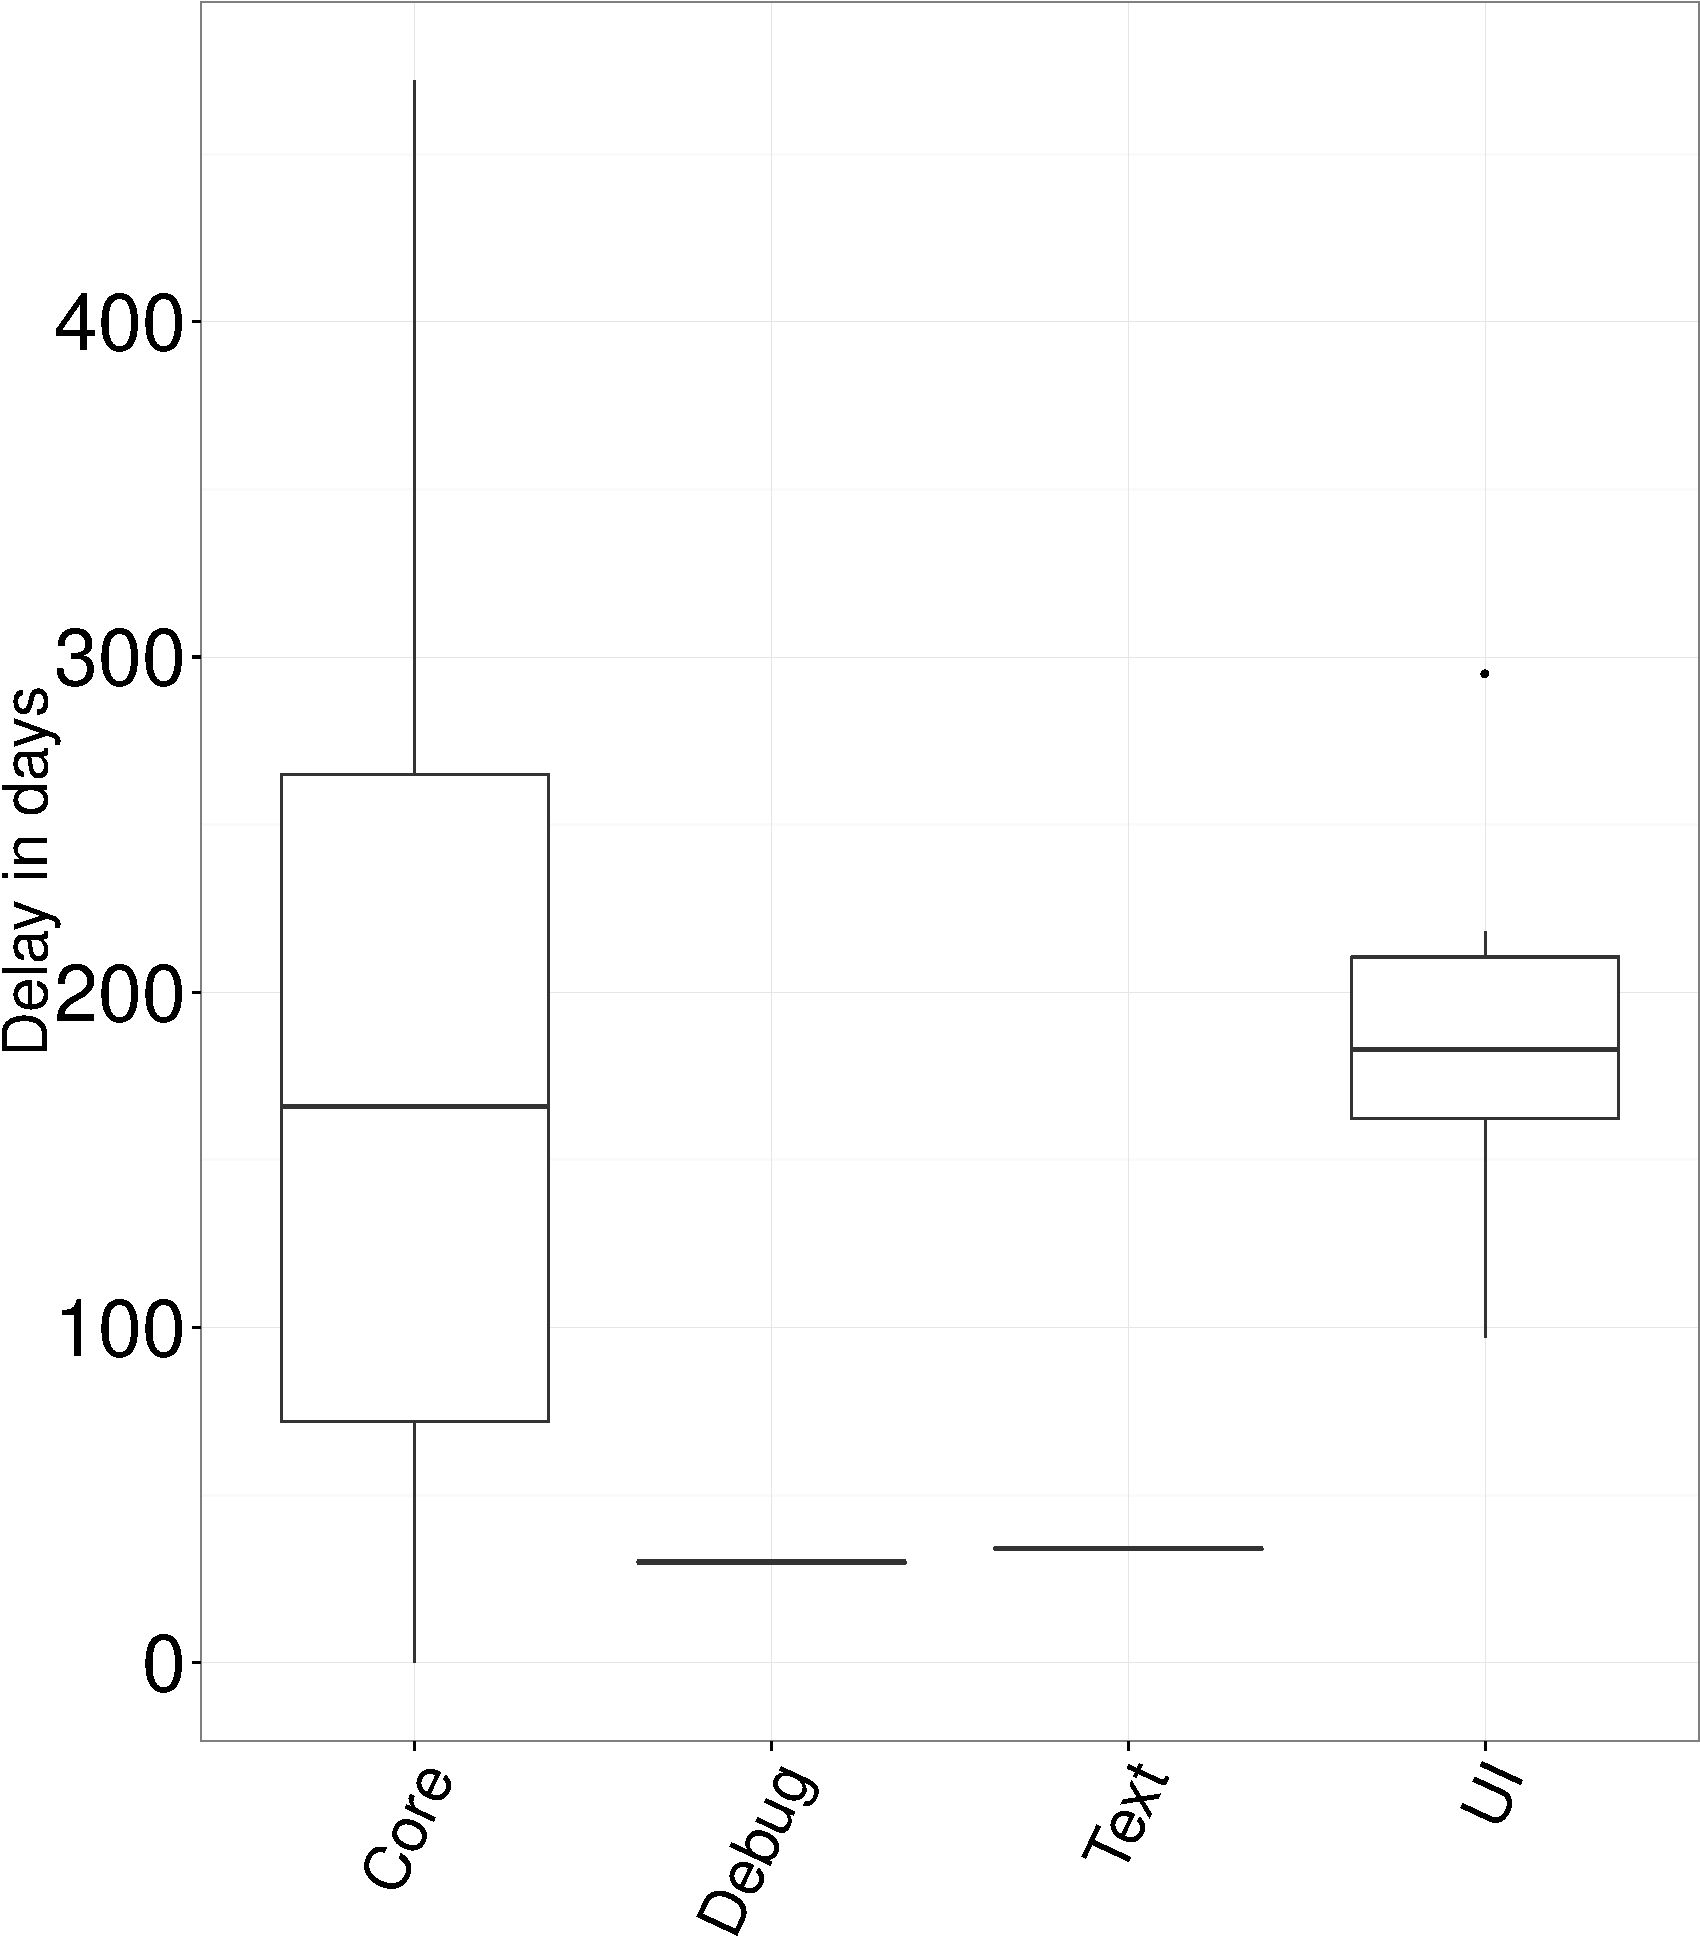
\includegraphics[width=0.40\textwidth,keepaspectratio]
		{chapters/chapter4/figures/components_eclipse.pdf}
	}

	\subfloat[Firefox]{
		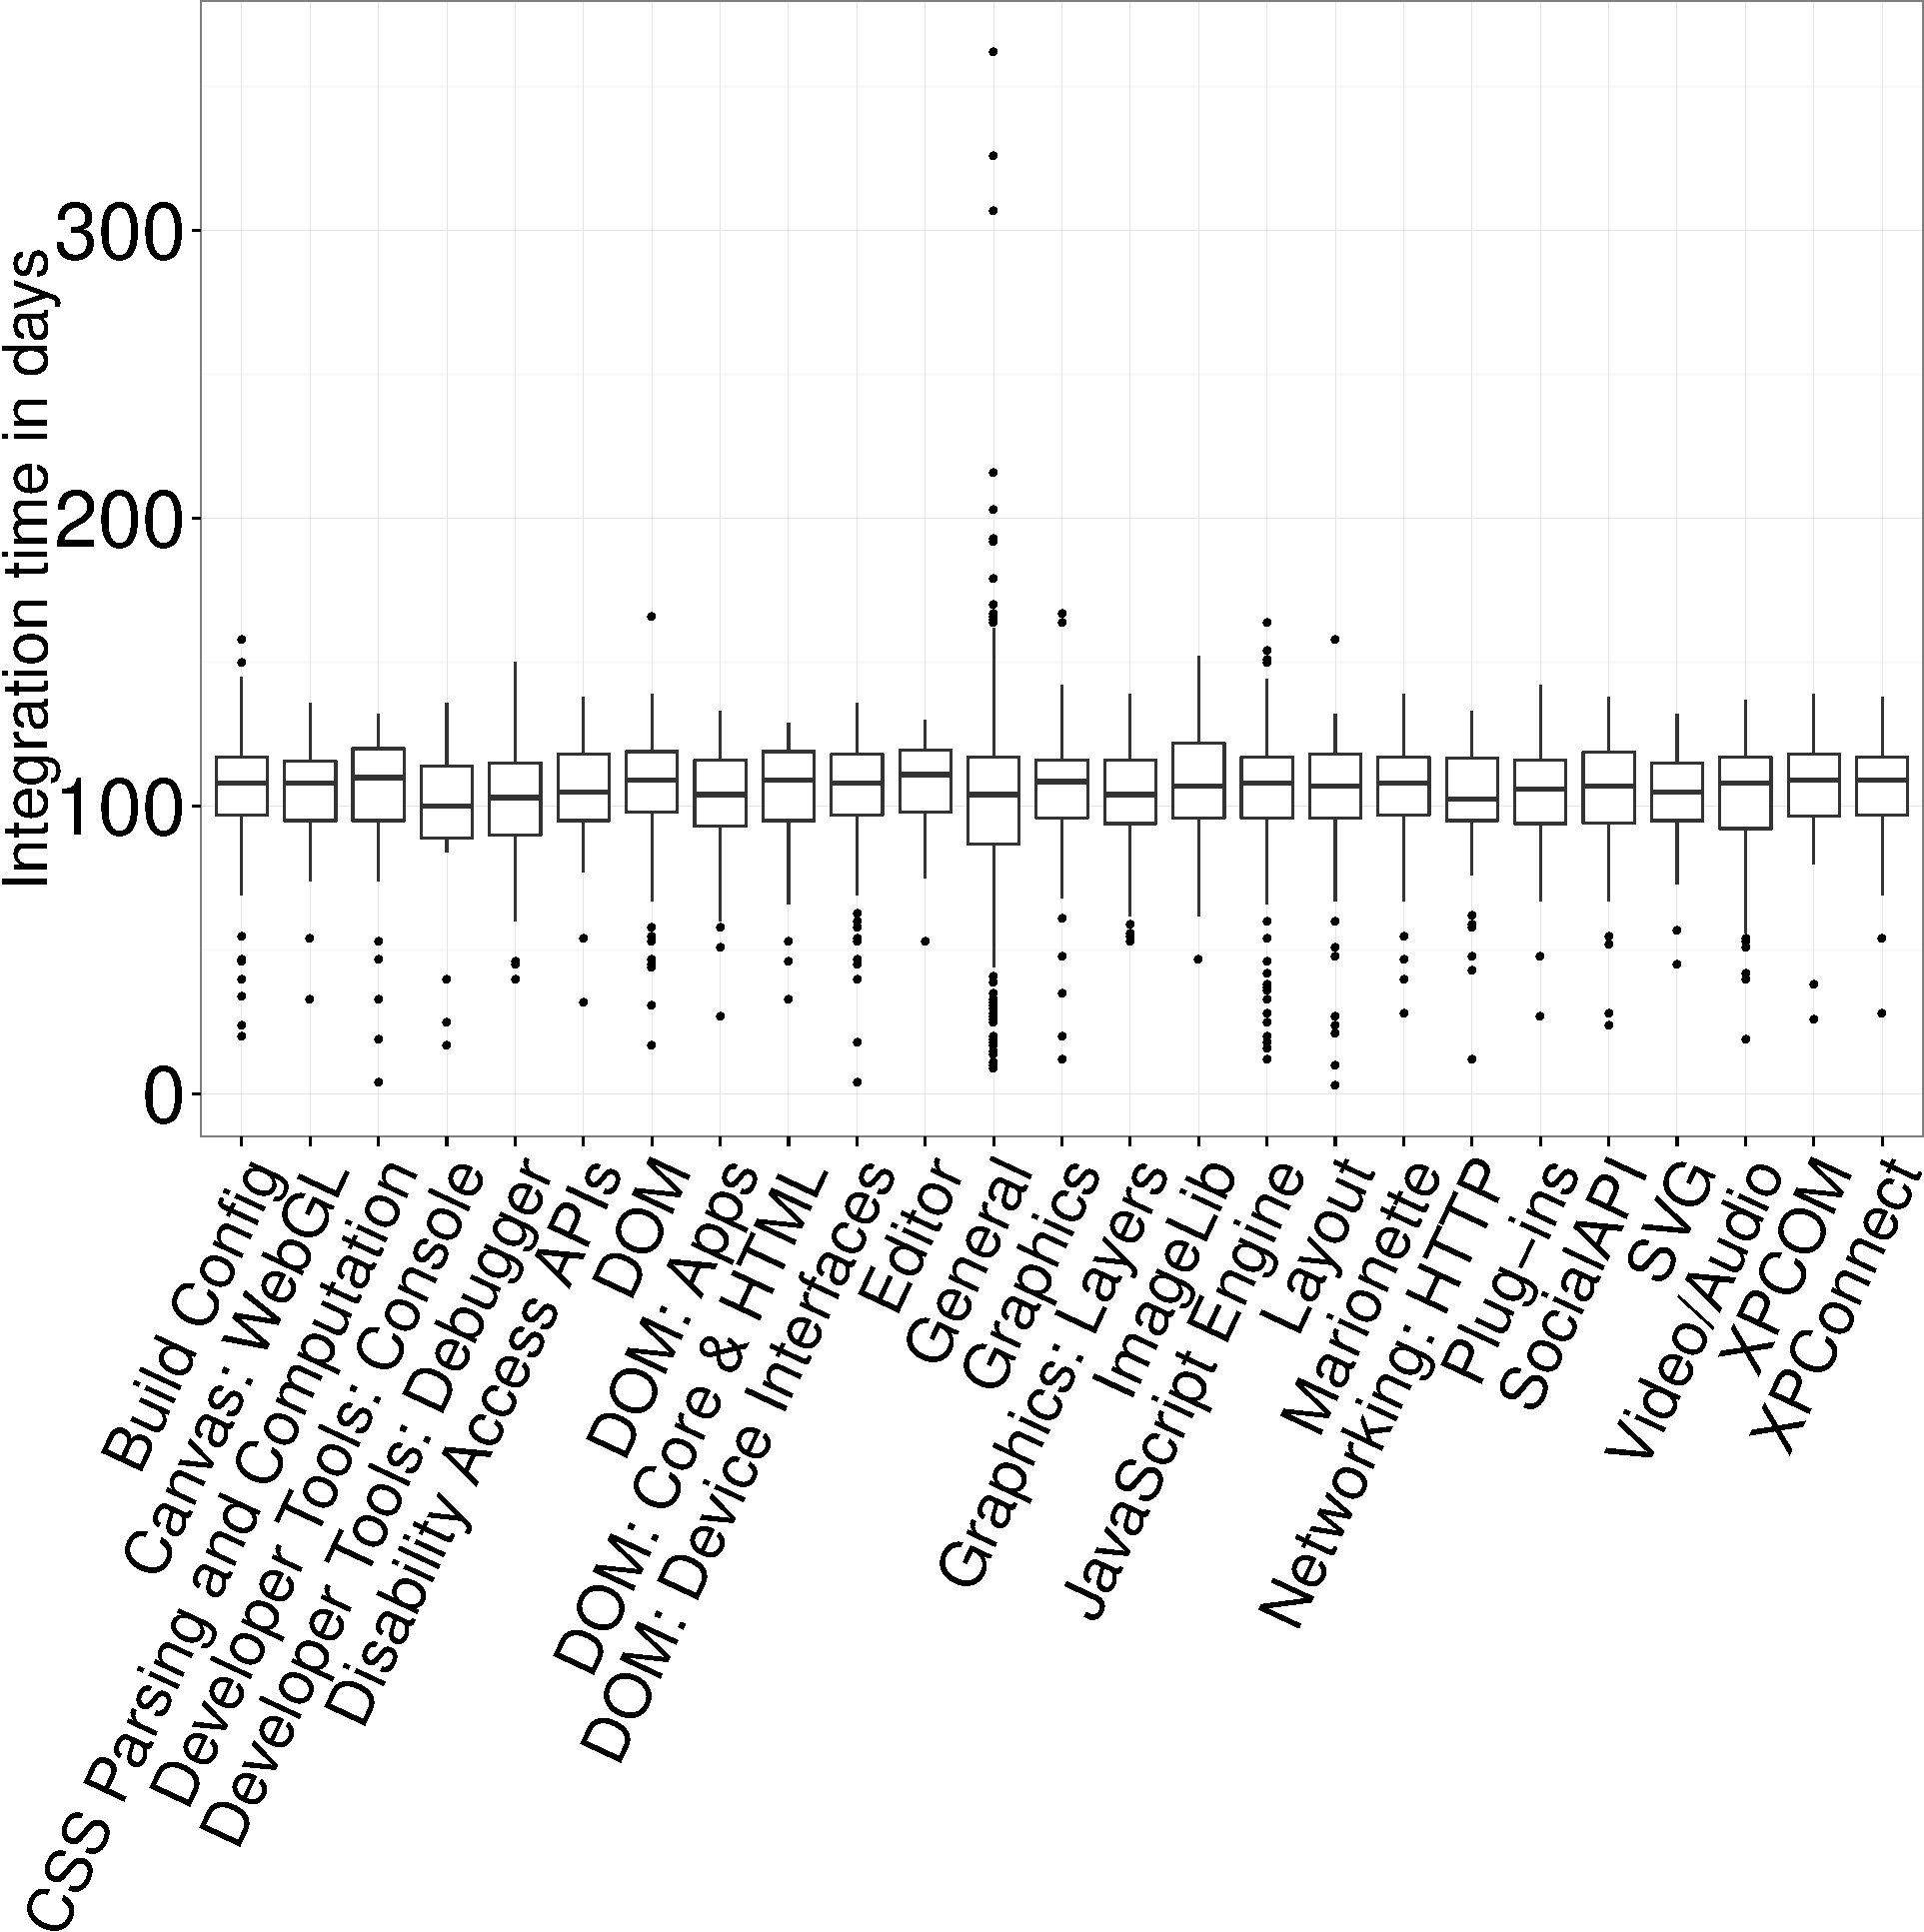
\includegraphics[width=0.40\textwidth,keepaspectratio]
		{chapters/chapter4/figures/components_firefox.pdf}
	}

	\subfloat[ArgoUML]{
		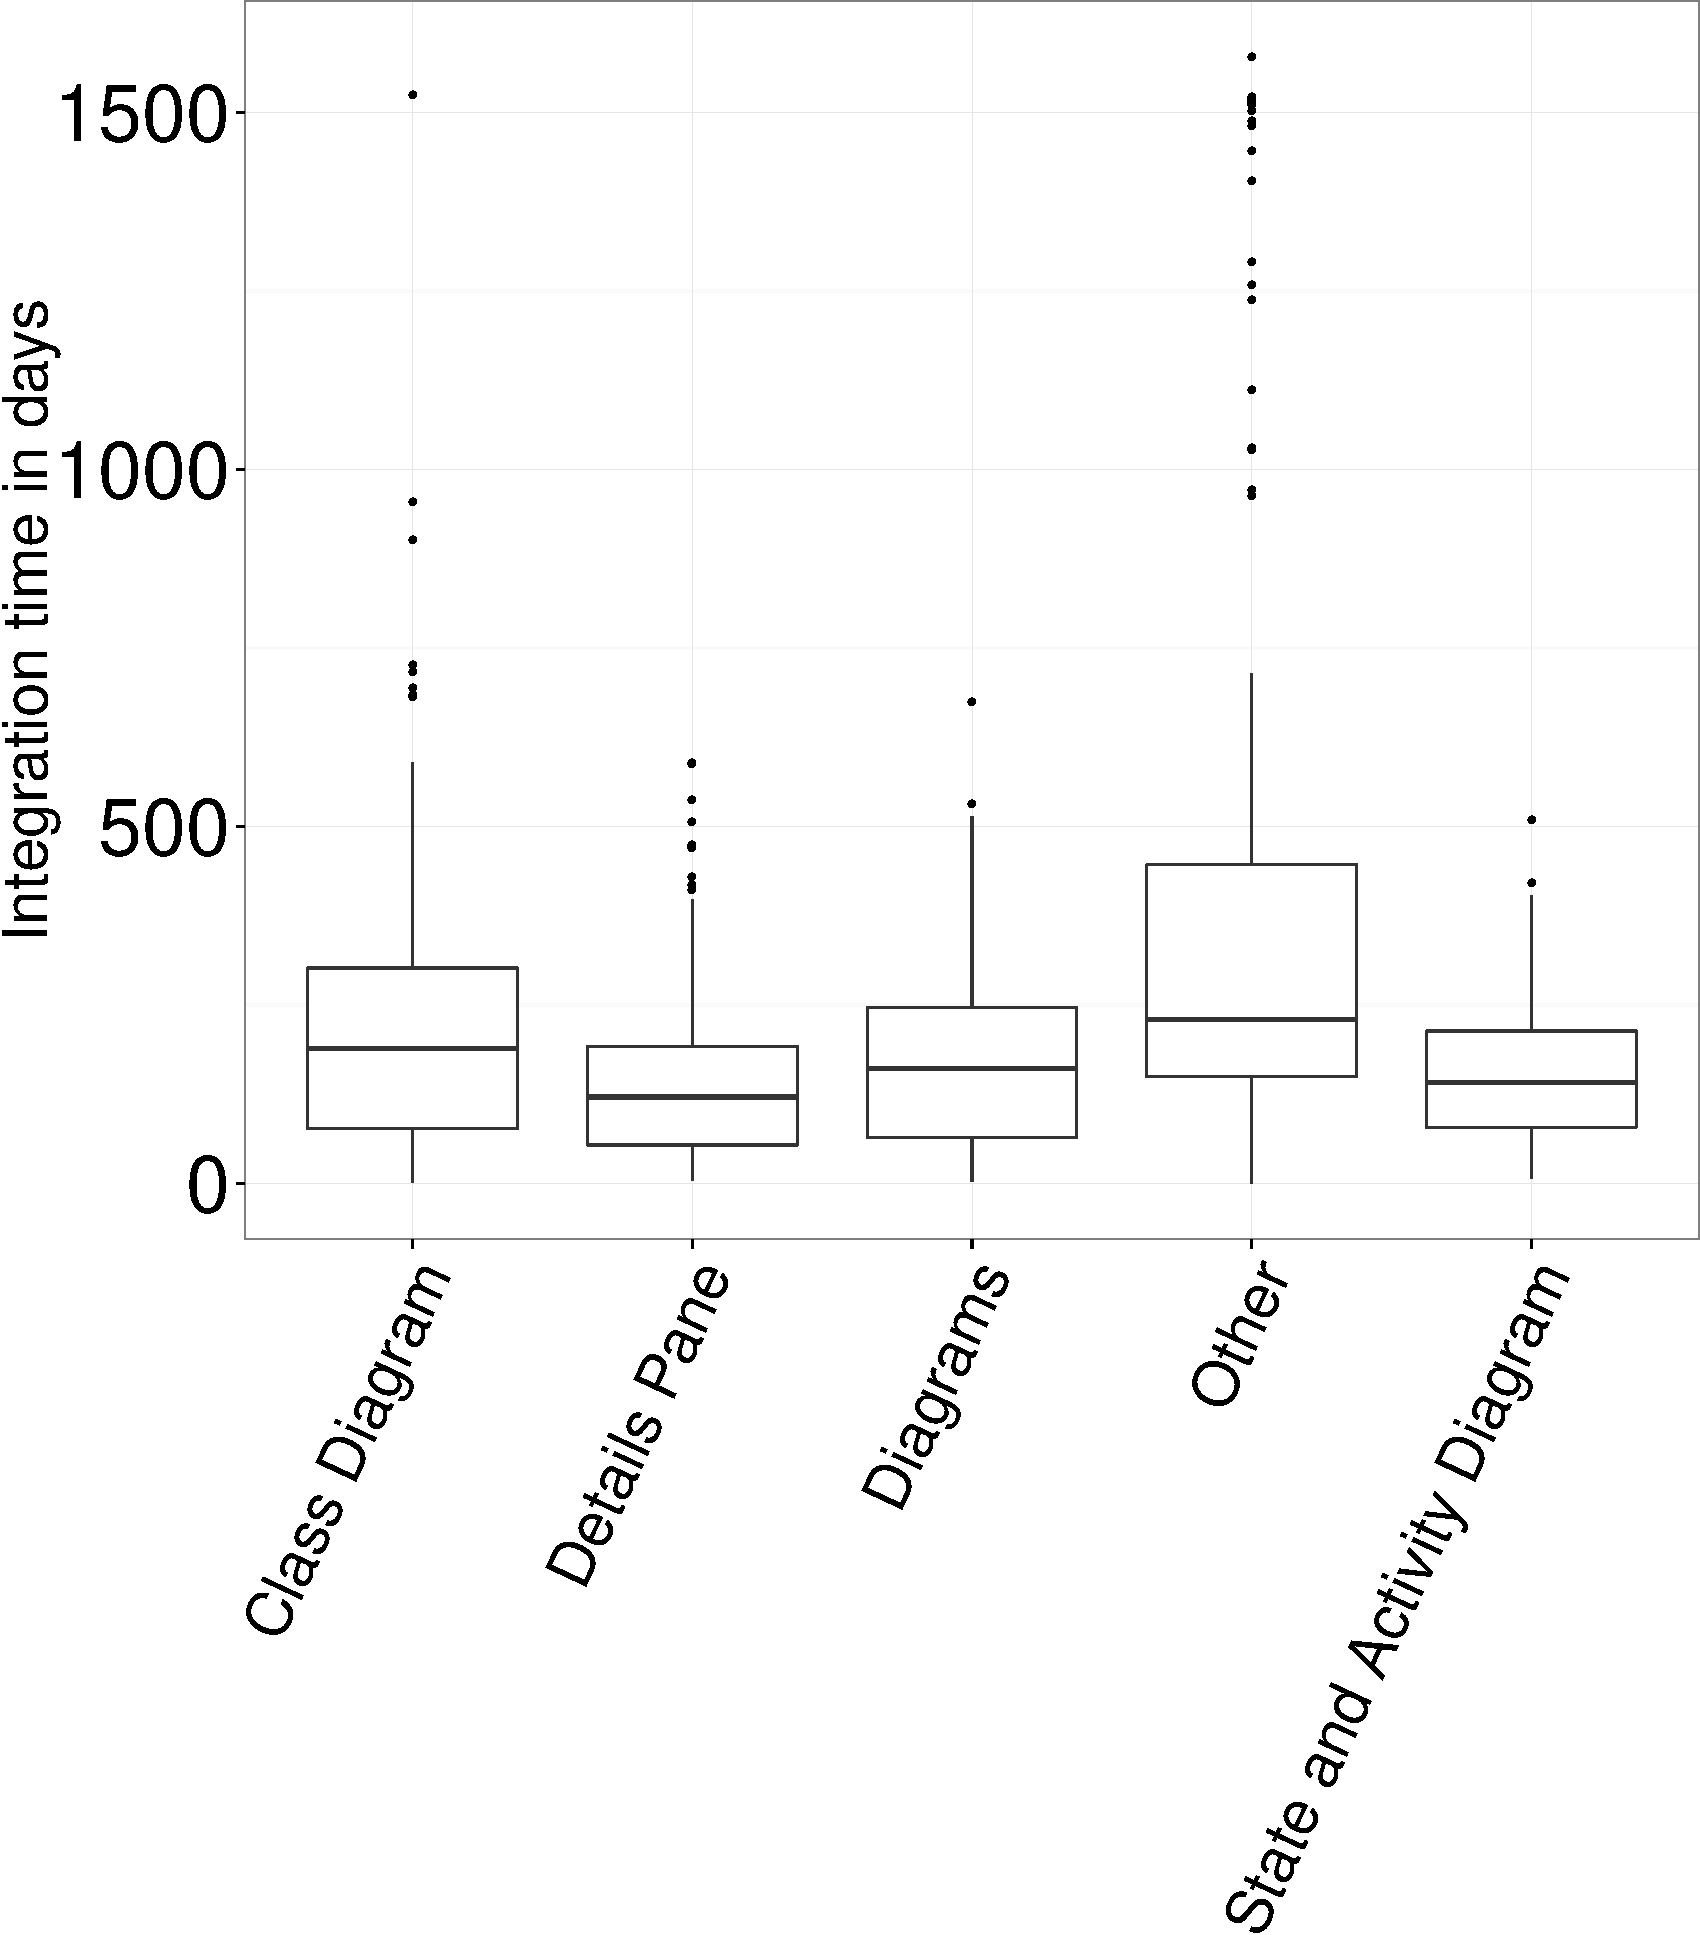
\includegraphics[width=0.40\textwidth,keepaspectratio]
		{chapters/chapter4/figures/components_argouml.pdf}
	}
	\caption{\textbf{Delivery delay per component.} The Figure shows the
		distributions of delivery delay in terms of days for each
		component of the studied projects.
	}
	\label{ch4:fig:component_analysis}
\end{figure}

\noindent\finding{The component to which an issue is addressed has little
impact in the delivery delay in terms of days.}{find13} To demonstrate this, we group
each addressed issue according to the components that such an issue modifies. We use
components that have at least 100 addressed issues as a threshold for our analysis.
We then compare the distribution of delivery delay in terms of days in these
components.
\hyperref[ch4:fig:component_analysis]{Figure}~\ref{ch4:fig:component_analysis} shows the
distributions of delivery delay in terms of days per component. We do not
observe a considerable difference between distributions of delivery delay in
the ArgoUML or Firefox projects. The distribution of the ``Other'' component in
the ArgoUML project is more skewed, which is suggestive of its generic
role---such a component may encompass a more broad spectrum of addressed issues. On
the other hand, 99\% of the addressed issues in the Eclipse (JDT) project belong to
the ``Core'' component (thus its skewness). Finally, the ``Debug'' and ``Text''
Eclipse components contain only one addressed issue each.   

\conclusionbox{The workload in terms of backlog of issues awaiting integration
	and the integration speed of prior addressed issues of a given resolver play
	a important role to model delivery delay in terms of days. Moreover,
	the initial \textit{queue position} is the most important attribute in
	all models that we fit to study delivery delay in terms of days.}

\subsection{RQ5: How well can we identify the addressed issues
that will suffer from a prolonged delivery delay?}\label{ch4:rq5}

\subsubsection*{RQ5: Motivation} 

End users may get frustrated if an addressed issue that s/he is interested has a
prolonged delivery delay. Furthermore, if such a delivery delay is unexpected for a
particular system (\eg it is very long), the frustration of users may increase
considerably, since they are not used to such a delivery delay. In
\hyperref[ch4:rq5]{RQ5} we
investigate if we can accurately identify which addressed issues are likely to
have a prolonged delivery delay. This investigation helps us mitigate the problem of
prolonged delivery delay of addressed issues.

\subsubsection*{RQ5: Approach} We calculate prolonged delivery delay
(\hyperref[def:3]{Definition}~\ref{def:3}) as
described in the \hyperref[settings:step3]{Step 3} of our data collection
process. Indeed, in
\hyperref[ch4:fig:beanplot_days]{Figure}~\ref{ch4:fig:beanplot_days}, we observe that
the distribution of delivery delay of the Eclipse and ArgoUML projects have more variation than
the distribution of the Firefox project.

The hexbin plots of \hyperref[ch4:fig:hexbins]{Figure}~\ref{ch4:fig:hexbins} show the
relationship between the delivery delay in terms of releases and days. Hexbin
plots are scatterplots that represent several data points with hexagon-shaped
bins. The lighter the shade of the hexagon, the more data points that fall
within the bin. Indeed, \hyperref[ch4:fig:hexbins]{Figure}~\ref{ch4:fig:hexbins}
suggests that the longer the delivery delay in terms of days, the longer is
the delivery delay in terms of releases. This tendency is more clear in the
Eclipse and Firefox projects. On the other hand, in the ArgoUML project, we
observe addressed issues with a longer delivery delay in terms of releases but
with a shorter delivery delay in terms of days. For instance, we observe addressed
issues with a delivery delay of four releases that have a shorter delivery
delay in terms of days than addressed issues with a delivery delay of three
releases.  Such behaviour in the ArgoUML project may be explained by the skew in
the distance between the releases of this project ({\em cf.}
\hyperref[ch4:fig:releaseIntervals]{Figure}~\ref{ch4:fig:releaseIntervals}).

\begin{figure}[t]
	\centering
	\subfloat[Eclipse]{
		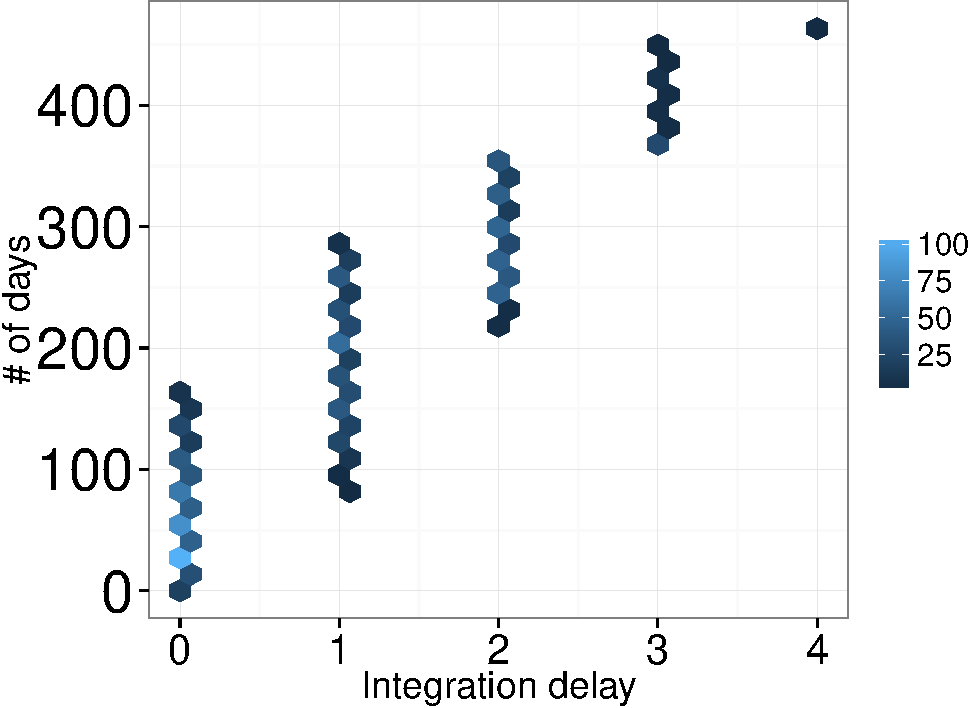
\includegraphics[width=0.49\textwidth,keepaspectratio]
		{chapters/chapter4/figures/eclipse_hexbinplot.pdf}
		\label{ch4:fig:eclipse_hexbin}
	}
	\subfloat[Firefox]{
		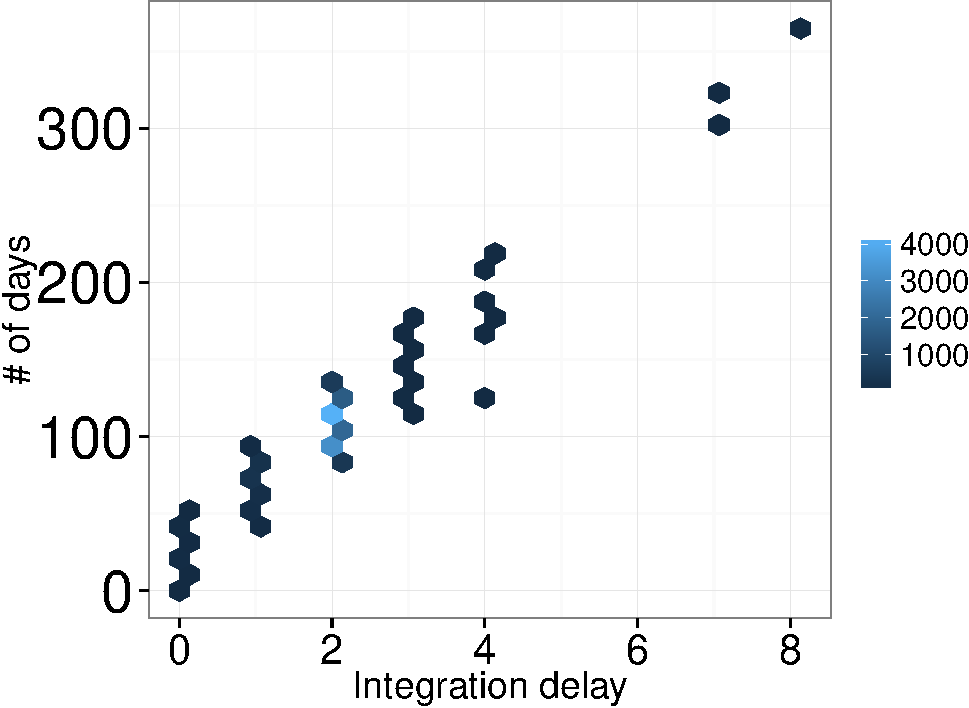
\includegraphics[width=0.49\textwidth,keepaspectratio]
		{chapters/chapter4/figures/firefox_hexbinplot.pdf}
		\label{ch4:fig:firefox_hexbin}
	}

	\subfloat[ArgoUML]{
		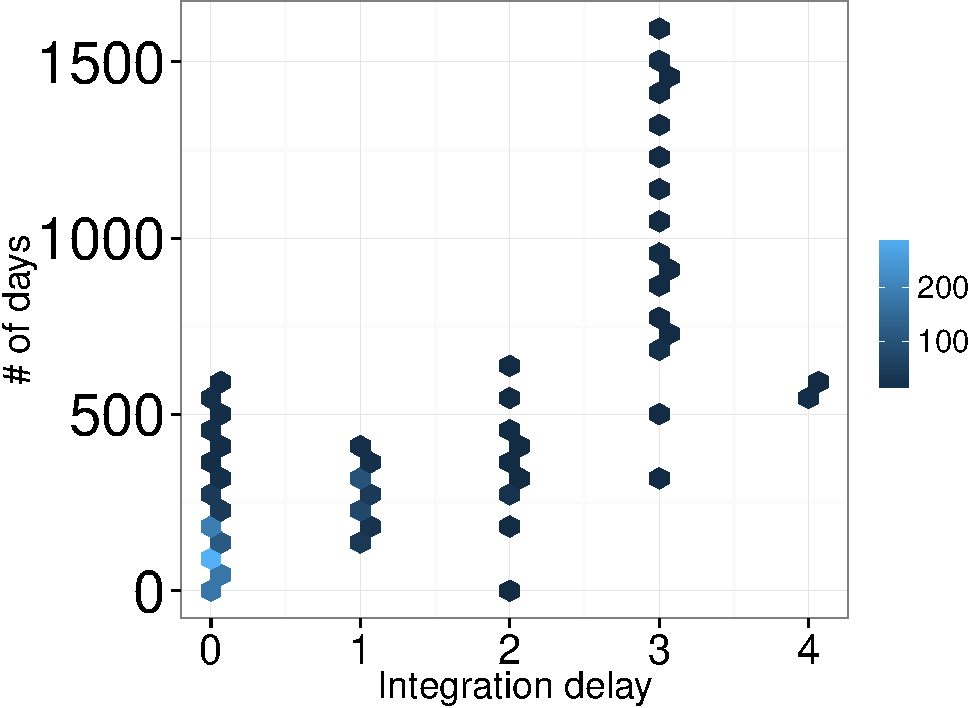
\includegraphics[width=0.49\textwidth,keepaspectratio]
		{chapters/chapter4/figures/argouml_hexbinplot.pdf}
		\label{ch4:fig:argouml_hexbin}
	}
	\caption{\textbf{Relationship between delivery delay in terms of
		releases and days.} We observe that
		a longer delivery delay in terms of releases is associated with a
	longer delivery delay in terms of days.}
	\label{ch4:fig:hexbins}
\end{figure}

\begin{figure}
	\centering
	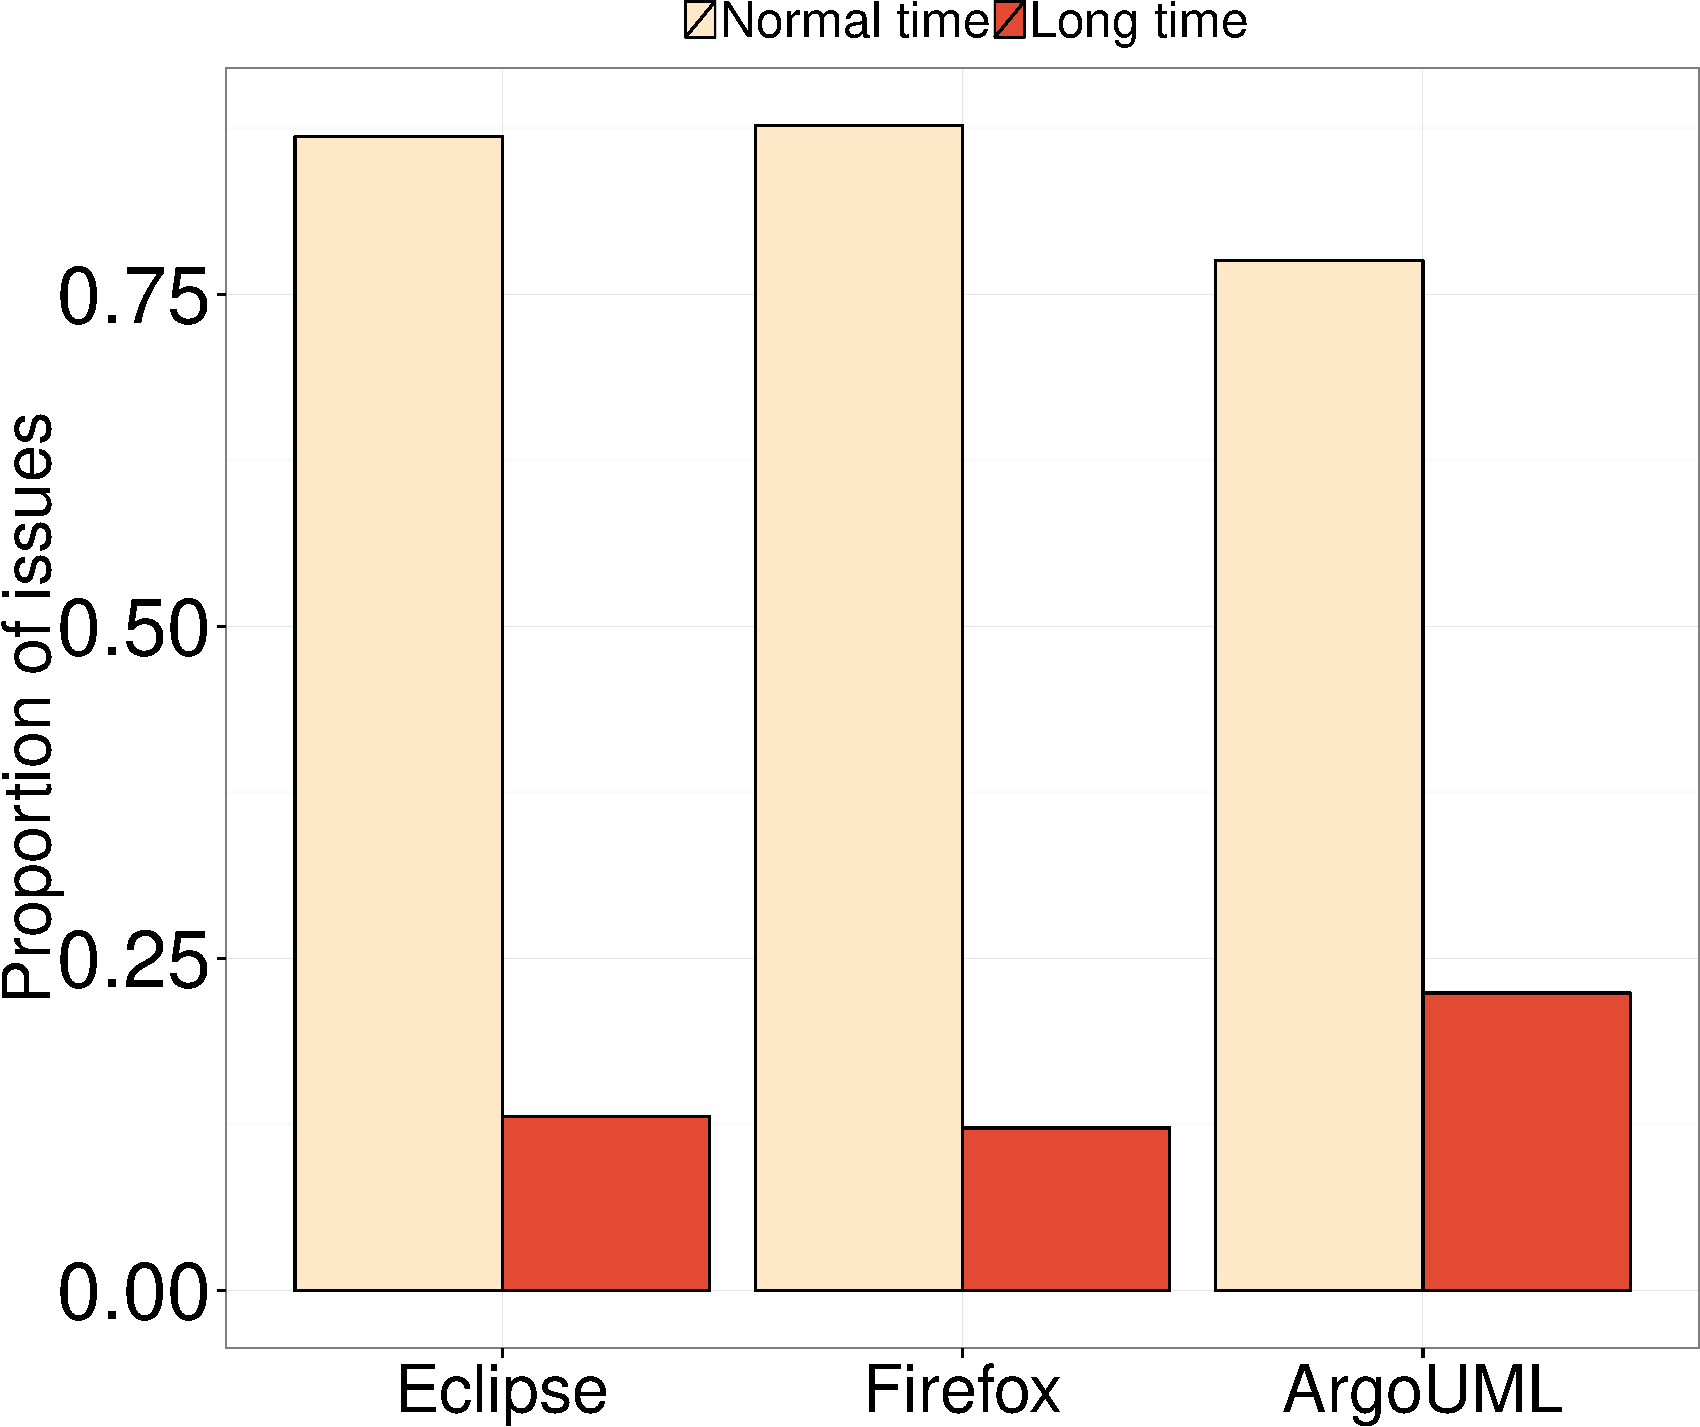
\includegraphics[width=0.80\textwidth,keepaspectratio]
	{chapters/chapter4/figures/largelydelayed_issues_per_project.pdf}
	\caption{\textbf{Addressed issues that have a prolonged delivery delay.} We present
		the proportion of addressed issues that have a prolonged
		delivery delay per project. 13\%, 12\%, and 22\% of the addressed issues
		of the Eclipse, Firefox, and ArgoUML projects have a prolonged
		delivery delay, respectively.}
		\label{ch4:fig:largely_delayed_issues}
	\end{figure}

\hyperref[ch4:tbl:median_plus_mad]{Table}~\ref{ch4:tbl:median_plus_mad} shows
the medians and MADs for each project to identify addressed issues that have a
prolonged delivery delay. For instance, an addressed issue have a prolonged
delivery delay in the Firefox project when that issue takes more than 123 days
to be delivered.
\hyperref[ch4:fig:largely_delayed_issues]{Figure}~\ref{ch4:fig:largely_delayed_issues}
shows the proportion of issues that have a prolonged delivery delay per project.
We observe that 13\%, 12\%, and 22\% of the addressed issues in the Eclipse,
Firefox, and ArgoUML projects have a prolonged delivery delay, respectively. 

\begin{table}[t!]
	\footnotesize
	\centering
	\caption{\textbf{Prolonged delivery delay thresholds.} We present the median
	delivery delay in terms of days, the MAD, and the prolonged delivery delay threshold for each project.}
	\label{ch4:tbl:median_plus_mad}
	\begin{tabular}{lrrr}
		\cline{2-4} 
		\multicolumn{1}{c}{} & \textbf{Eclipse} & \textbf{Firefox} &
		\textbf{ArgoUML}\tabularnewline
		\hline 
		\textbf{Median delivery delay} & 166 & 107 & 146\tabularnewline
		\hline 
		\textbf{Median absolute deviation} & 142 & 16 & 131\tabularnewline
		\hline 
		\textbf{Prolonged delivery delay} & $>$ 308 & $>$ 123 & $>$ 278\tabularnewline
		\hline 
	\end{tabular}
\end{table}

To train our exploratory models, we produce a dichotomous response variable $Y$,
where $Y=1$ means that an addressed issue has a prolonged delivery delay, while $Y=0$
means that the delivery delay of that issue is normal. Finally, we train
random forest models to study whether a given addressed issue is likely to have a
prolonged delivery delay. Similar to \hyperref[ch4:rq2]{RQ2}, we evaluate our models
using \textit{precision}, \textit{recall}, \textit{F-measure}, and \textit{AUC}.

\subsubsection*{RQ5: Results}

\noindent\finding{Our models obtain F-measures from 0.79 to 0.96.}{find14}
\hyperref[ch4:tbl:RFclassificationResult_ab]{Table}~\ref{ch4:tbl:RFclassificationResult_ab}
shows the performance of our exploratory models. Our models that we train for
the Eclipse project obtain the highest F-measure (0.96). On the other hand, our
models trained for the Firefox and ArgoUML projects obtain F-measures of 0.79
and 0.88, respectively. Moreover, our models obtain AUC values of 0.82 to 0.96.
Such results suggest that our models vastly outperform na\"{i}ve models, such as
random guessing (AUC value of 0.50).  \\

\begin{table}[t!]
	\footnotesize
	\centering
	\caption{\textbf{Performance of the random forest models.} The table
		shows the values of Precision, Recall, F-measure, and AUC values that
	are computed for the LOOCV of our models.}
	\label{ch4:tbl:RFclassificationResult_ab}
	\begin{tabular}{lccc}
		\cline{2-4} 
		& \textbf{Eclipse} & \textbf{Firefox} & \textbf{ArgoUML}\tabularnewline
		\hline 
		\textbf{Precision} & 0.97 & 0.99 & 0.98\tabularnewline
		\hline 
		\textbf{Recall} & 0.96 & 0.66 & 0.80\tabularnewline
		\hline 
		\textbf{F-measure} & 0.96 & 0.79 & 0.88\tabularnewline
		\hline 
		\textbf{AUC} & 0.96 & 0.82 & 0.89\tabularnewline
		\hline 
	\end{tabular}
\end{table}

\noindent\finding{Our models obtain better F-measure values than
Zero-R.}{find15} For the Eclipse, Firefox, and ArgoUML projects, Zero-R obtain median F-measures
of 0.22, 0.22, and 0.36, respectively. Meanwhile, our explanatory models obtain
F-measures of 0.96, 0.79, and 0.88, respectively. Again, such results suggest
that our models vastly outperform na\"{i}ve classification techniques.  \\

\conclusionbox{
We are able to accurately identify whether an addressed issue is likely to have
a long delivery delay in a given project. Our models outperform na\"{i}ve
techniques, such as Zero-R and random guessing, obtaining AUC values from 0.82
to 0.96 (median).
}

\subsection{RQ6: What are the most influential attributes for                        
	identifying the issues that will suffer from a prolonged delivery delay?}\label{ch4:rq6}                                                                    
                                                                                    
\subsubsection*{RQ6: Motivation} RQ6 shows that we can accurately                    
identify whether an addressed issue is likely to have a prolonged delivery delay.         
However, it is also important to understand what attributes are more influential    
when identifying addressed issues with prolonged delivery delay, \ie from which attributes 
do our models derive the most explanatory power?                                    
                                                                                    
\subsubsection*{RQ6: Approach} Similar to \hyperref[ch4:rq4]{RQ4}, in this research
question, we analyze our explanatory models by computing the variable importance
score of the attributes.                                                                         

\subsubsection*{RQ6: Results}

\begin{figure}
	\centering
	\subfloat[Eclipse]{
		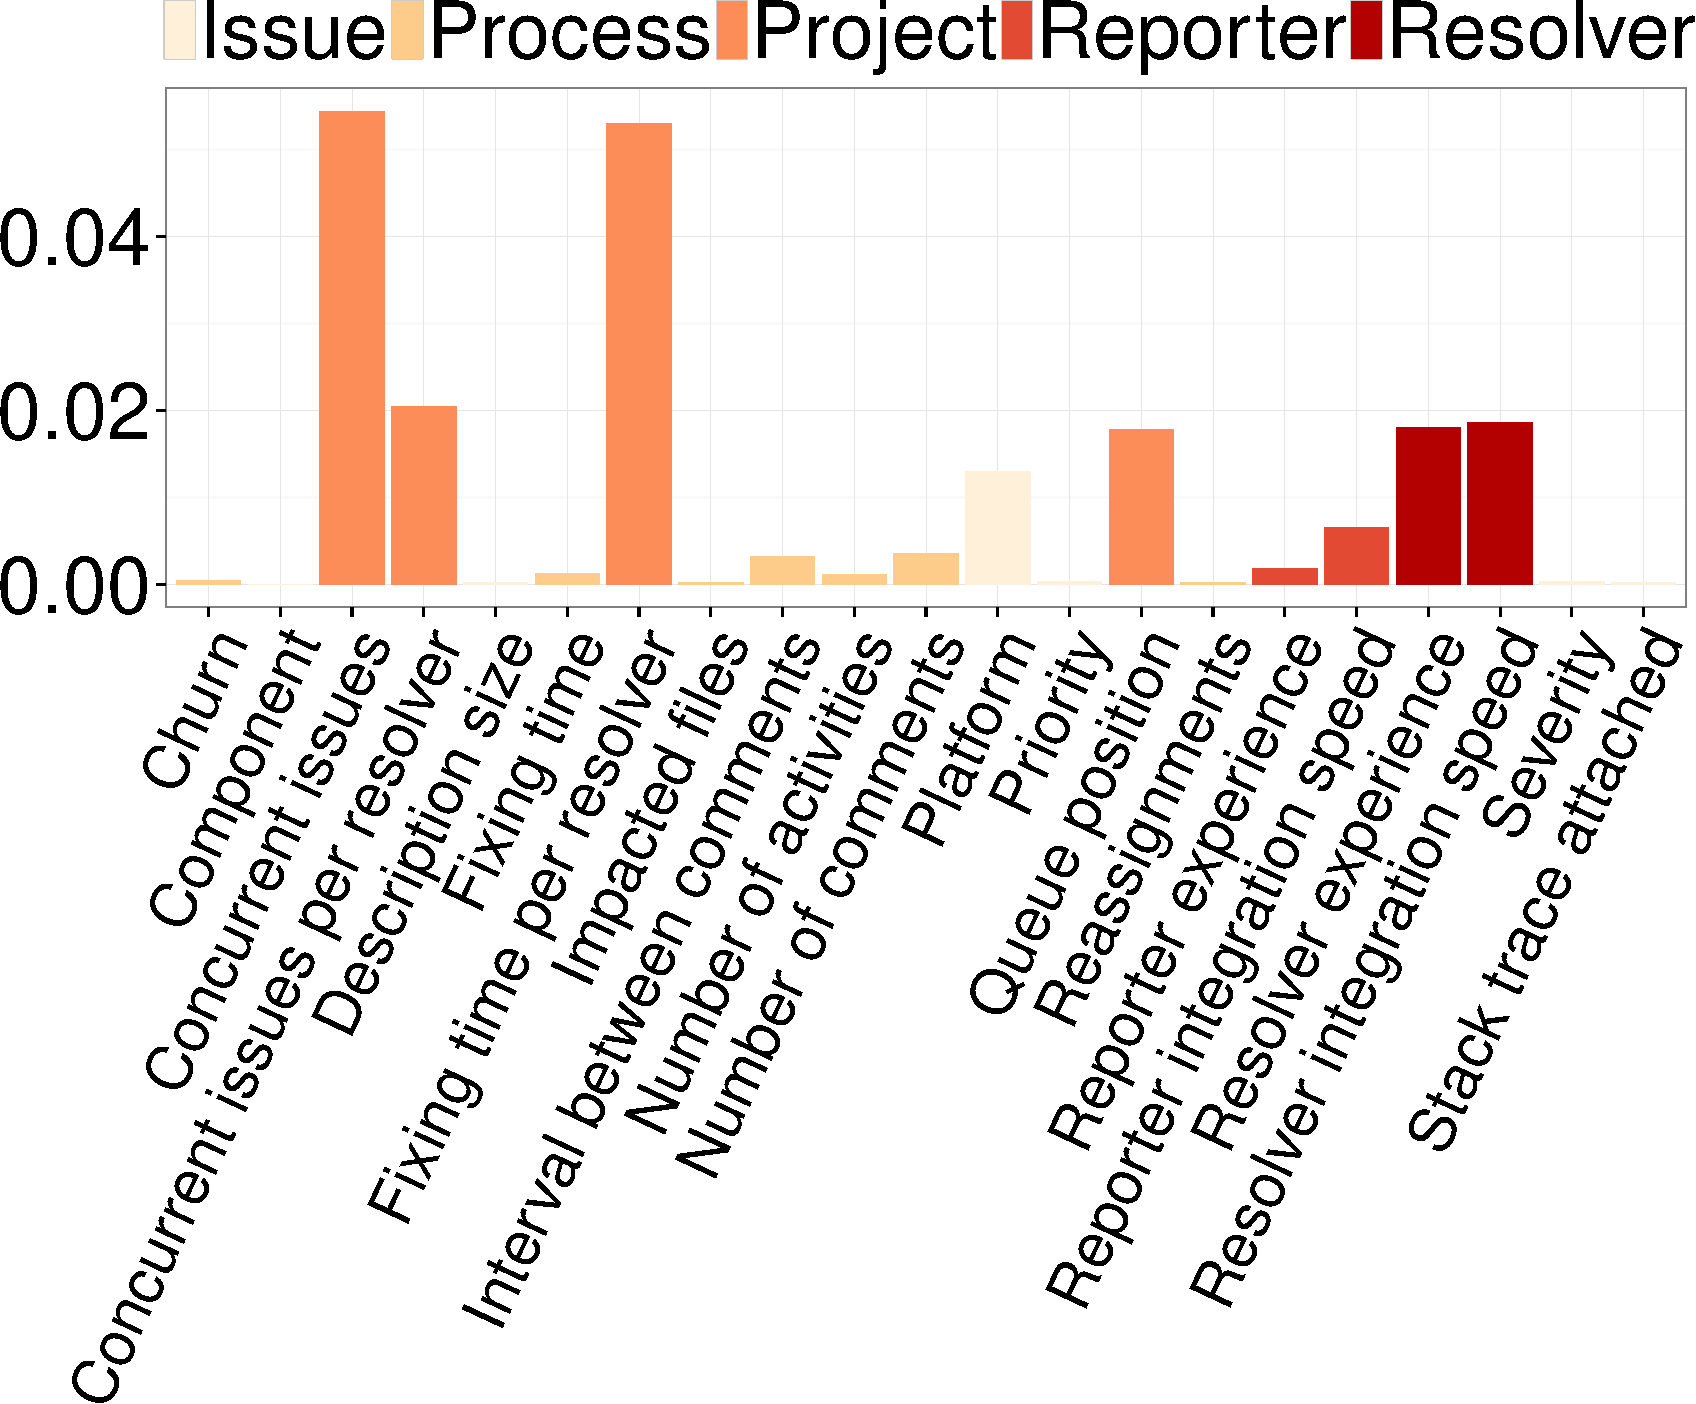
\includegraphics[width=0.50\textwidth,keepaspectratio] 
		{chapters/chapter4/figures/eclipse_loocv_varimp_long.pdf}
	\label{ch4:fig:impEclipse_ab}}

	\subfloat[Firefox]{
		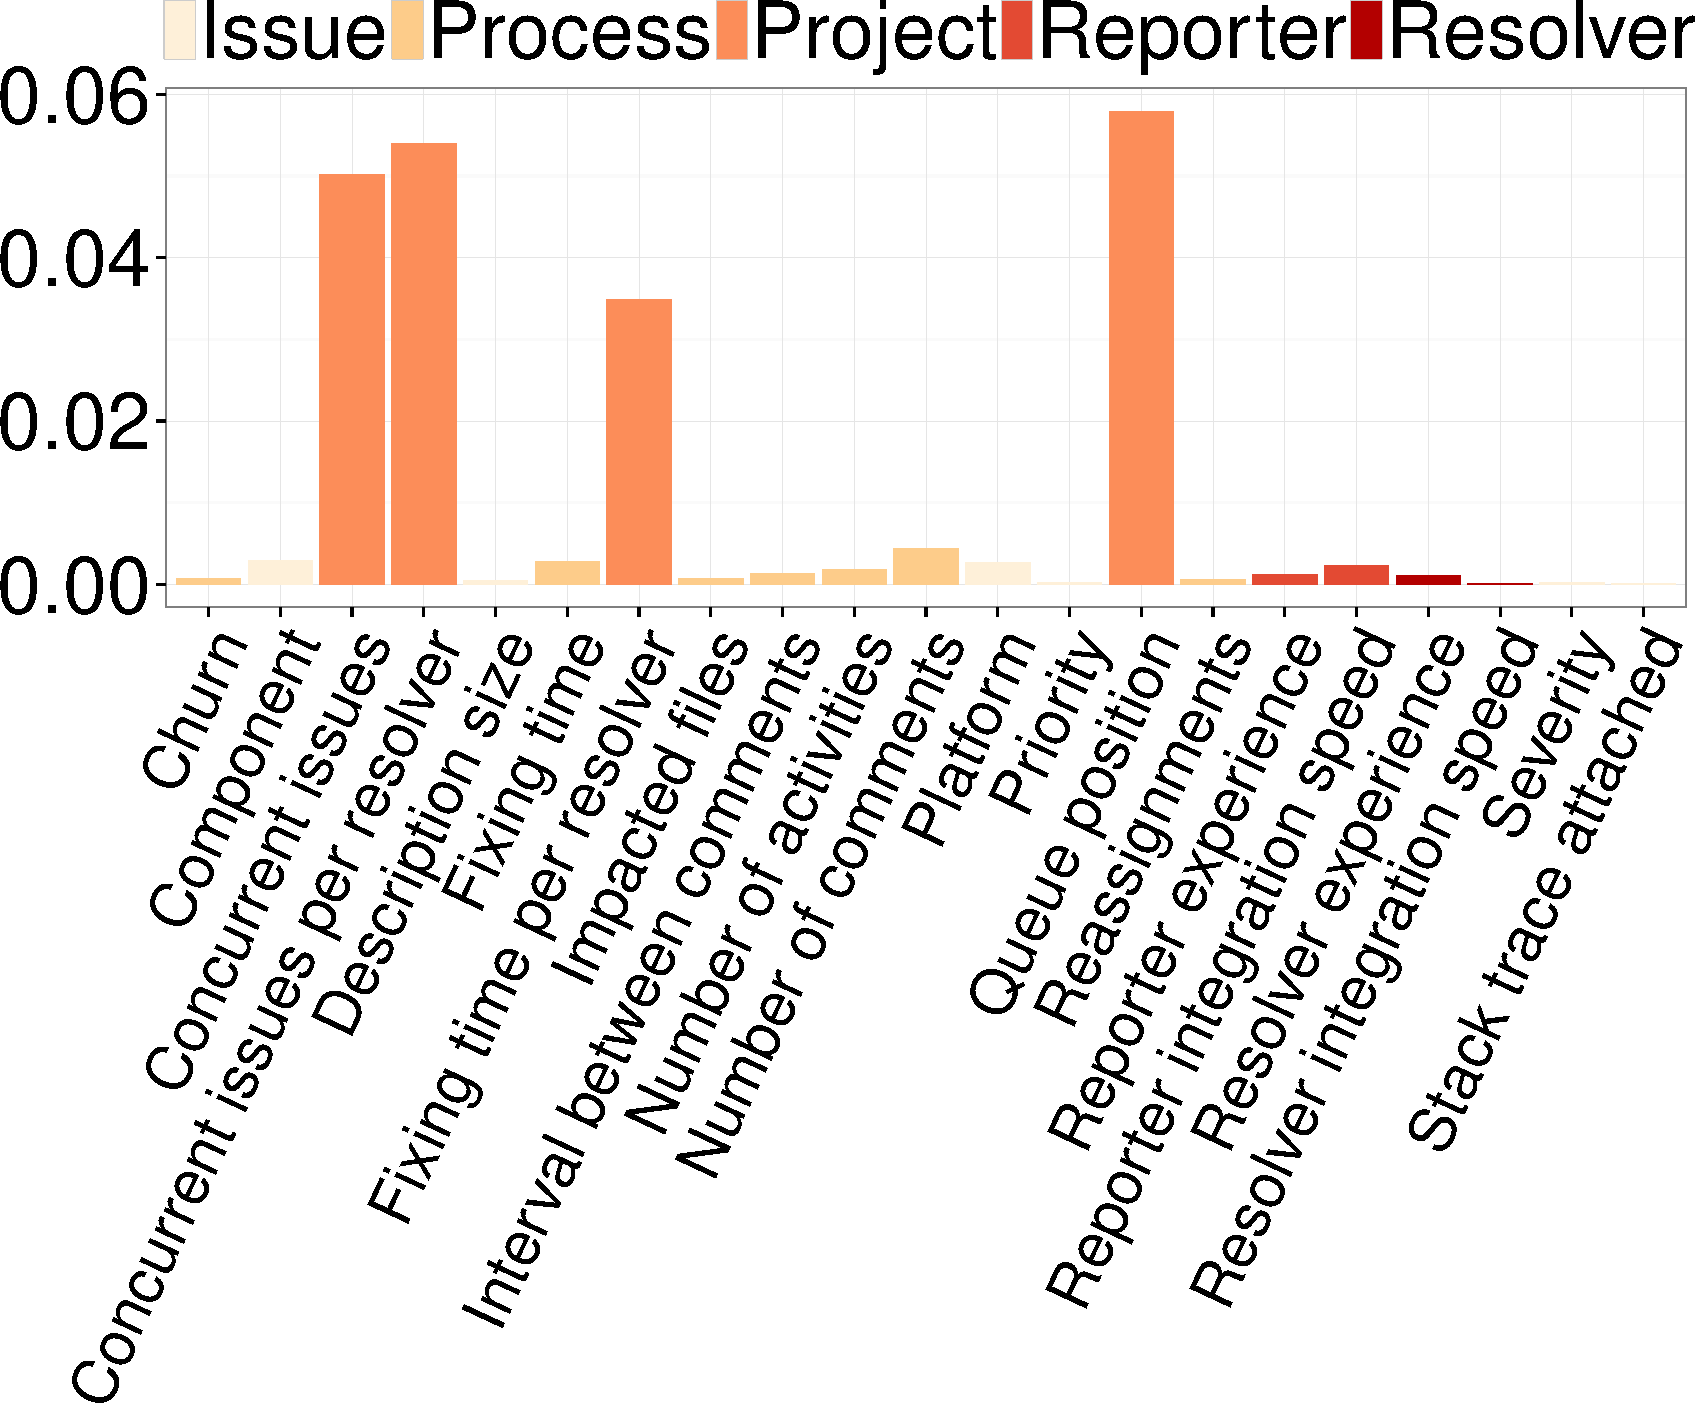
\includegraphics[width=0.50\textwidth,keepaspectratio]  
		{chapters/chapter4/figures/firefox_loocv_varimp_long.pdf}
		\label{ch4:fig:impFirefox_ab}
	}

	\subfloat[ArgoUML]{
		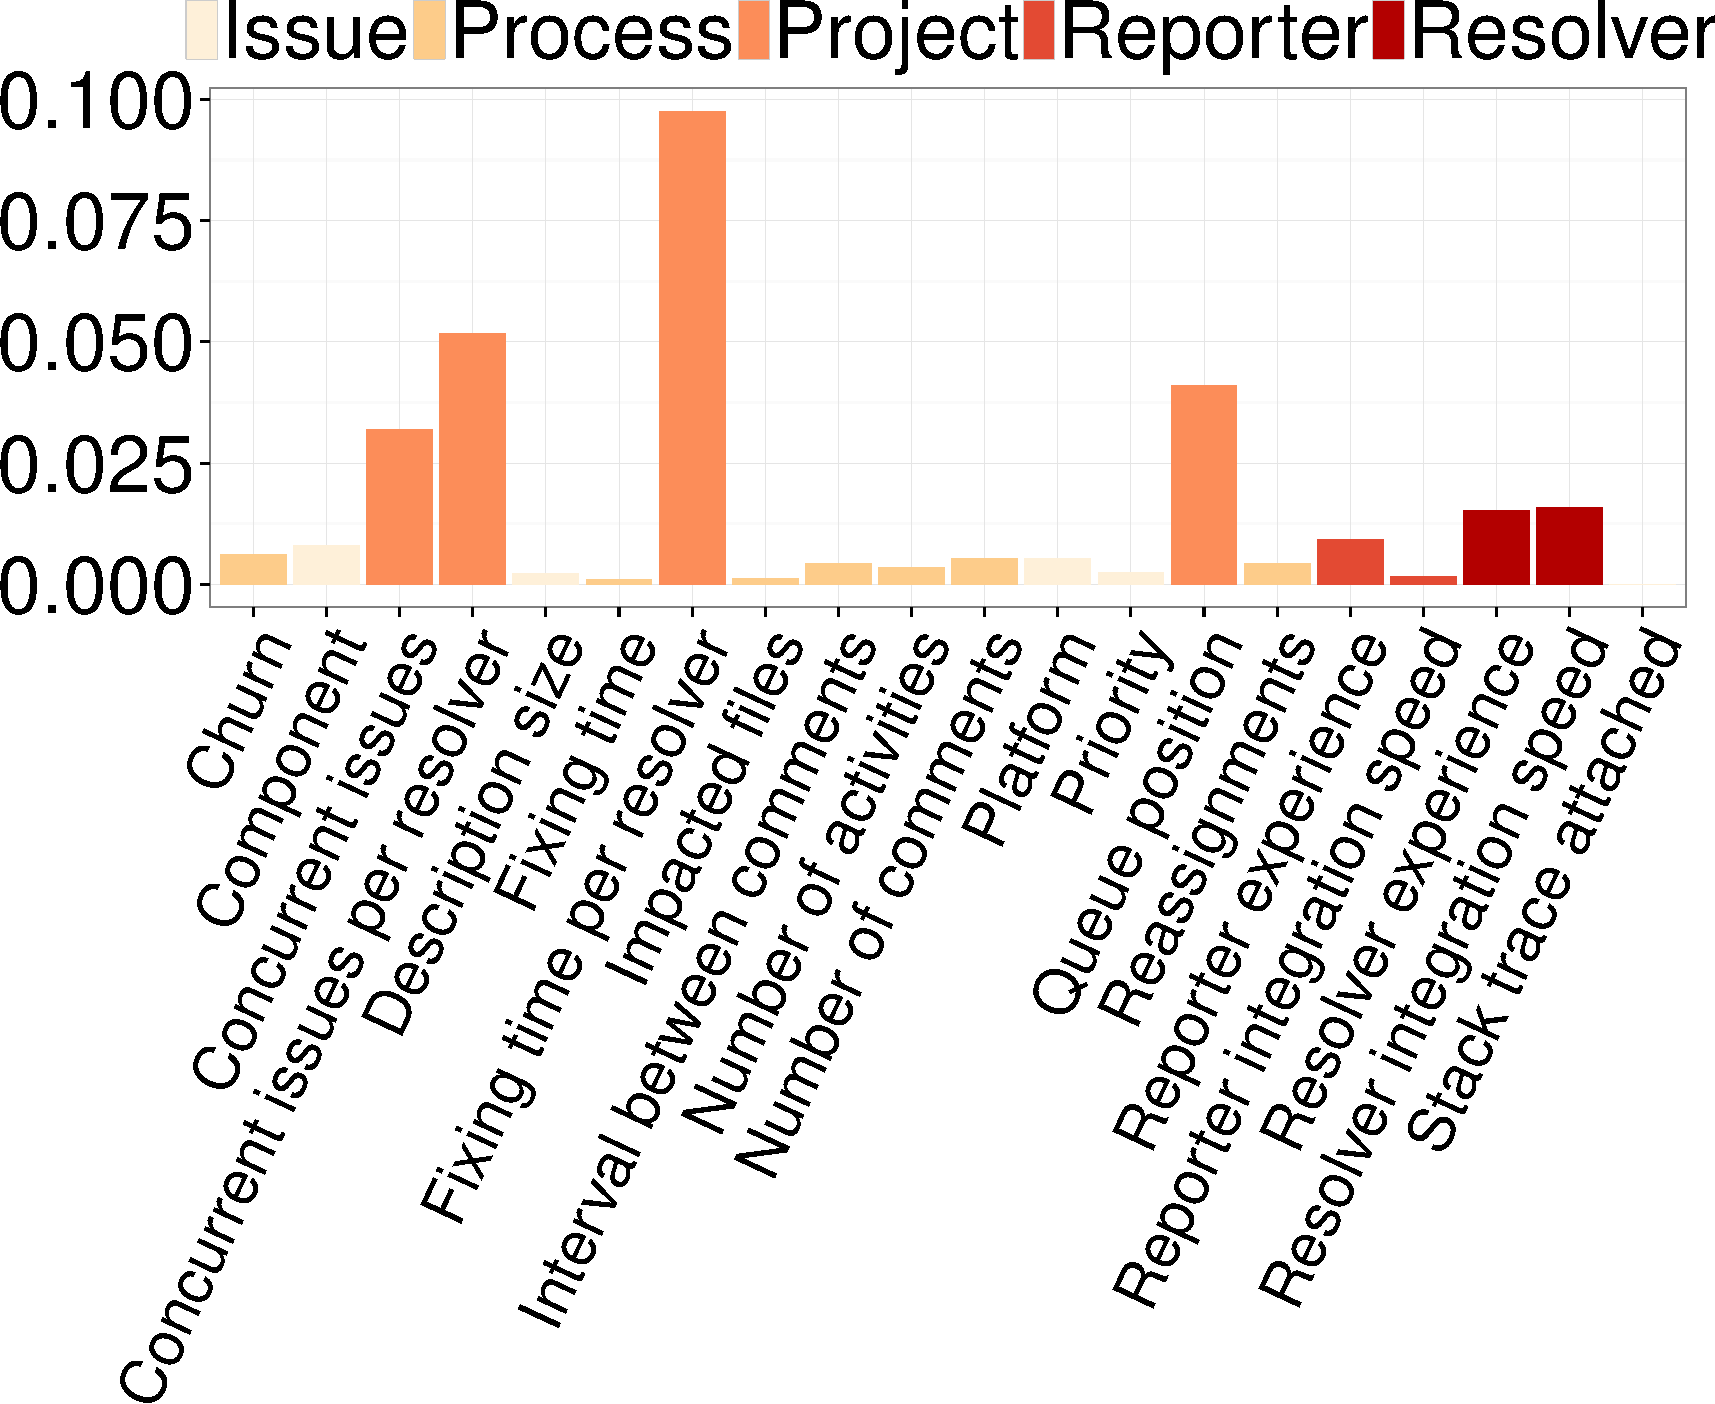
\includegraphics[width=0.50\textwidth,keepaspectratio] 
		{chapters/chapter4/figures/argouml_loocv_varimp_long.pdf}
	\label{ch4:fig:impArgo}}
	\caption{\textbf{Variable importance scores.} We show the 
	importance scores that are computed for the LOOCV of our models.}
	\label{ch4:fig:variableImportance_ab}
\end{figure}


\noindent\finding{Prolonged delivery delay is most consistently associated with
attributes of the project family.}{find16}

\hyperref[ch4:fig:variableImportance_ab]{Figure}~\ref{ch4:fig:variableImportance_ab}
shows the importance scores that are computed for the LOOCV that we use to
evaluate our random forest models. We observe that the attributes that are
related to the \textit{\textbf{project}} family are the most influential
attributes in the projects. The \textit{backlog of issues} is the most
influential attribute in our Eclipse models, while \textit{queue position} and
\textit{fixing time per resolver} are the most influential attributes in our
Firefox and ArgoUML models, respectively. In addition, we observe that
attributes that are related to workload, such as the \textit{backlog of issues}
and the \textit{backlog of issues per resolver} are at least the third most
influential attributes in all of our models. Such results suggest that a
\textit{prolonged delivery delay} is associated with project-related attributes and
that the amount of addressed issues that are to be delivered also plays a major
role to identify a \textit{prolonged delivery delay}. \\

\conclusionbox{Our explanatory models suggest that prolonged delivery delay is more
	closely associated with project characteristics, such as
	the \textit{backlog of issues}, \textit{queue position}, and
	\textit{fixing time per resolver}. Moreover, the backlog of issues plays an
	influential role in identifying a prolonged delivery delay in all of the studied
projects.}


%\section{Results for Study 1}\label{ch4:study1} 

In this section, we present the results with respect to the \textit{concrete
integration time} dimension. This dimension involves the investigation of
integration time in terms of number of releases and number of days
(\hyperref[def:1]{Definitions}~\ref{def:1} and \ref{def:2}). This dimension is
comprised of \hyperref[ch4:rq1]{RQ1}-\hyperref[ch4:rq4]{RQ4}. Below, we present the
obtained results for each RQ. 
%here goes RQ1, RQ2, and RQ3

\subsection*{\textit{\textbf{RQ1: How often are addressed issues prevented from being
released?}}}\label{resutls:rq1}

\begin{figure}[!t]
	\centering
	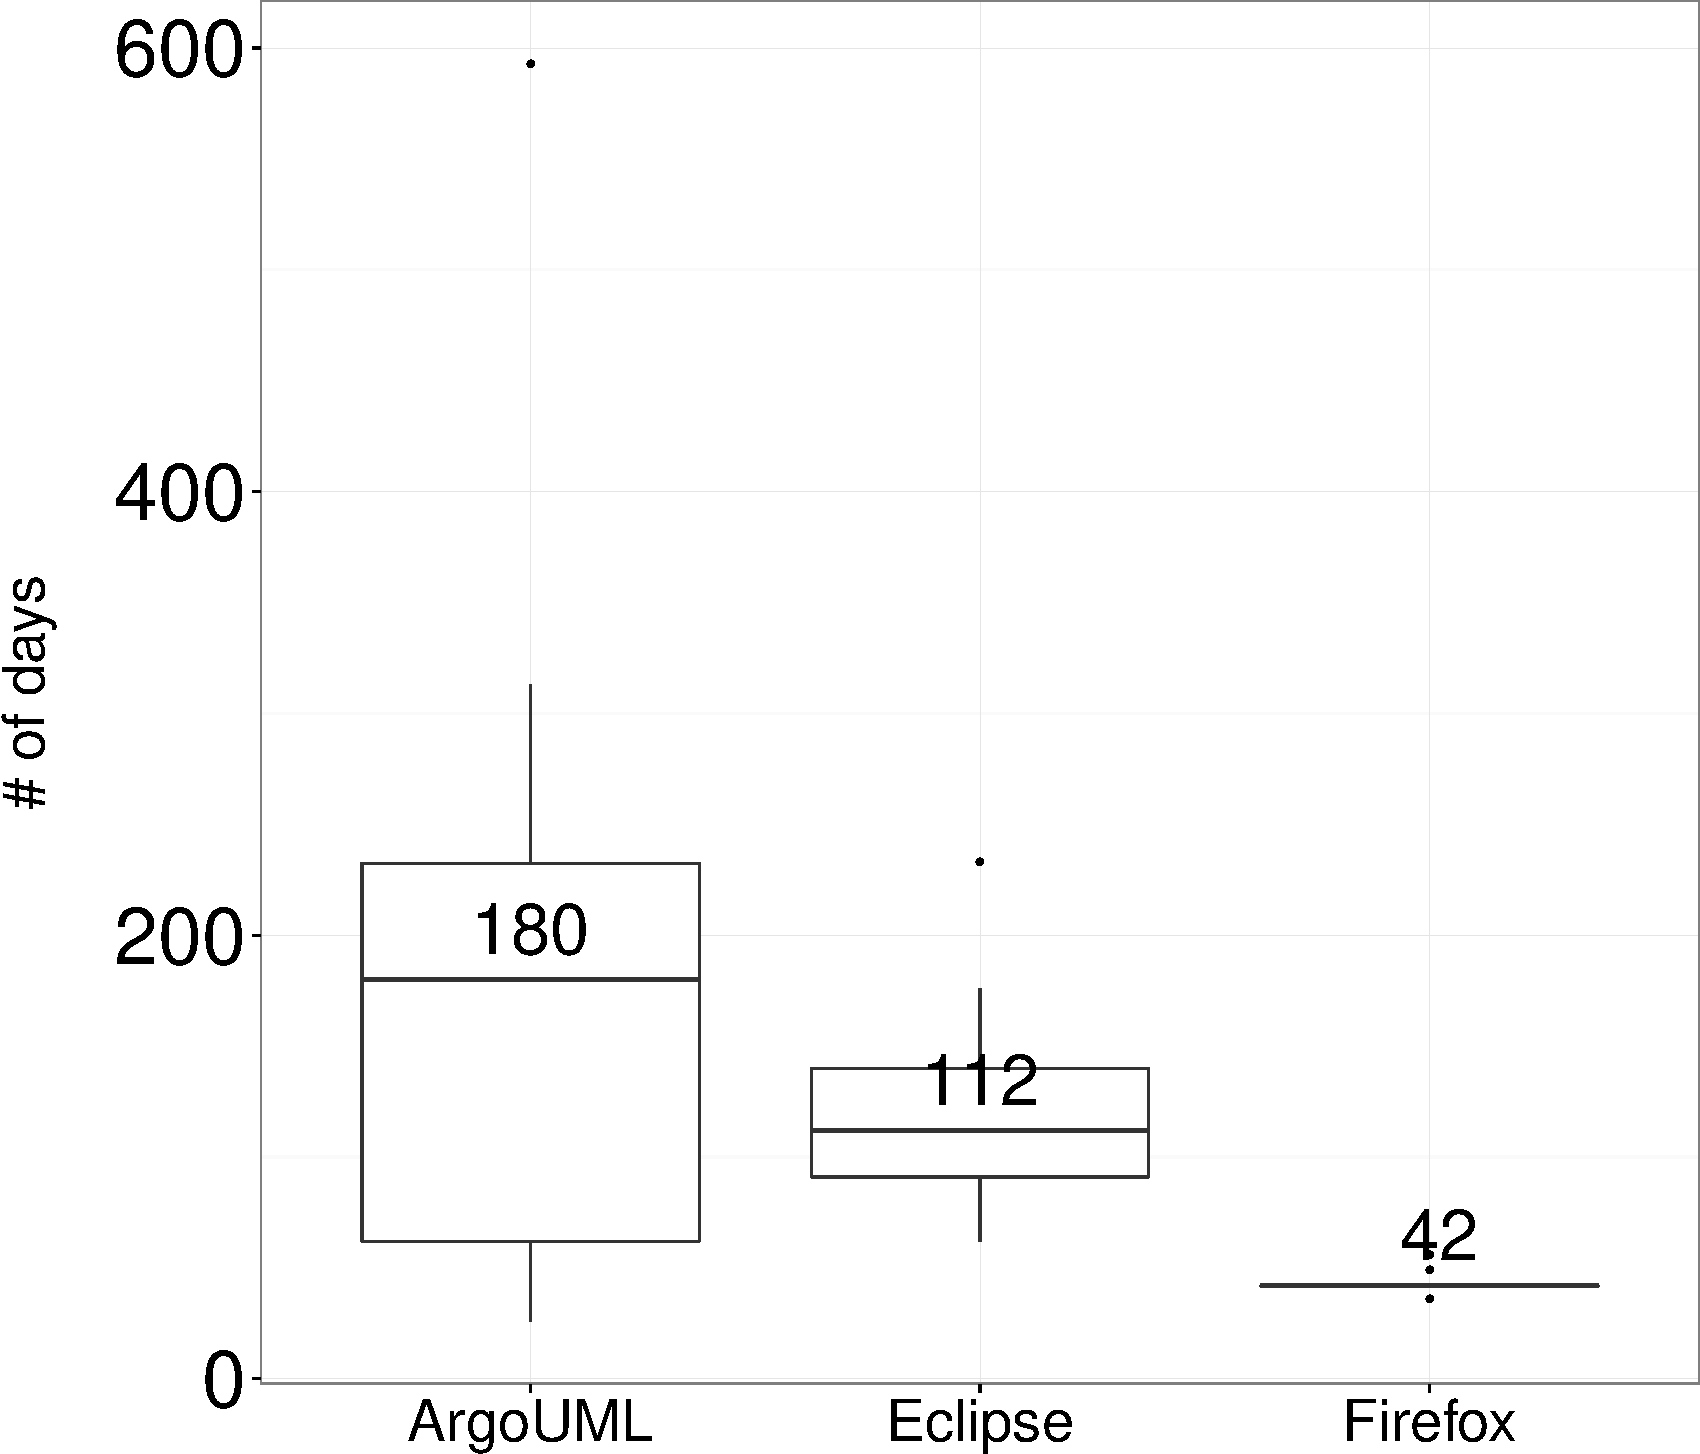
\includegraphics[width=0.7\textwidth]
	{chapters/chapter4/figures/RQ1_time_between_releases.pdf}
	\caption{\textbf{Number of days between the studied releases of the
	ArgoUML, Eclipse, and Firefox projects.} The number shown over each
boxplot is the median interval.}  
	\label{ch4:fig:releaseIntervals}
\end{figure}

\noindent\textit{\textbf{Addressed issues usually
miss the next release in the Firefox project.}}
\hyperref[ch4:fig:releaseIntervals]{Figure}~\ref{ch4:fig:releaseIntervals} shows the
difference between the studied projects in terms of the time interval between
their releases. The median time in days for the Firefox project (42 days) is
approximately $\frac{1}{4}$ that of the ArgoUML project (180 days), and
$\frac{1}{3}$ that of the Eclipse project (112 days). Unlike the Eclipse and
Firefox projects, the distribution for the ArgoUML project is skewed. In
addition, \hyperref[ch4:fig:fixToIntegration]{Figure}~\ref{ch4:fig:fixToIntegration}
shows that the vast majority of addressed issues for the Firefox project is integrated
\textit{after-2} releases, whereas for the Eclipse and ArgoUML projects, the
majority is integrated in the \textit{next} release. 

The reason for the difference may be due to the release policies that are
followed in each project. For example,
\hyperref[ch4:fig:releaseIntervals]{Figure}~\ref{ch4:fig:releaseIntervals} shows that
the Firefox project releases consistently every 42 days (six weeks), whereas the
time intervals between the releases of the ArgoUML project vary from 50 to 220
days. Indeed, the release guidelines for the ArgoUML project state that the
ArgoUML team should release at least one stable release every 8 months (see
\hyperref[argouml:releng]{Section}~\ref{argouml:releng}). The delivery
consistency of the Firefox releases might lead to addressed issues being prevented
from a greater number of releases, since the Firefox project rigidly adhere to a
six-week release schedule despite accumulating issues that could not be
integrated (see \hyperref[firefox:releng]{Section}~\ref{firefox:releng}). 

Although an addressed issue usually misses the next release in the Firefox
project, issues are usually shipped faster when compared to the other projects.
Indeed, \hyperref[ch4:fig:beanplot_days]{Figure}~\ref{ch4:fig:beanplot_days} shows that
addressed issues in the Firefox project take a median of 107 days to be
released, while it takes 166 and 146 days in the Eclipse and ArgoUML projects,
respectively.\\

\noindent\textit{\textbf{34\% to 60\% of addressed issues had their integration
prevented from at least one release in the traditionally released projects.}}
\hyperref[ch4:fig:fixToIntegration]{Figure}~\ref{ch4:fig:fixToIntegration} shows that
98\% of the addressed issues in the Firefox project are prevented from integration
in at least one release. However, for the projects that adopt a more traditional
release cycle, \ie the ArgoUML and Eclipse projects, 34\% to 60\%  of the addressed
issues are prevented from integration in at least one release. This result
indicates that even though an issue is addressed, integration may be prevented by
one or more releases, which can frustrate end users.\\

\begin{figure}[!t]
	\centering
	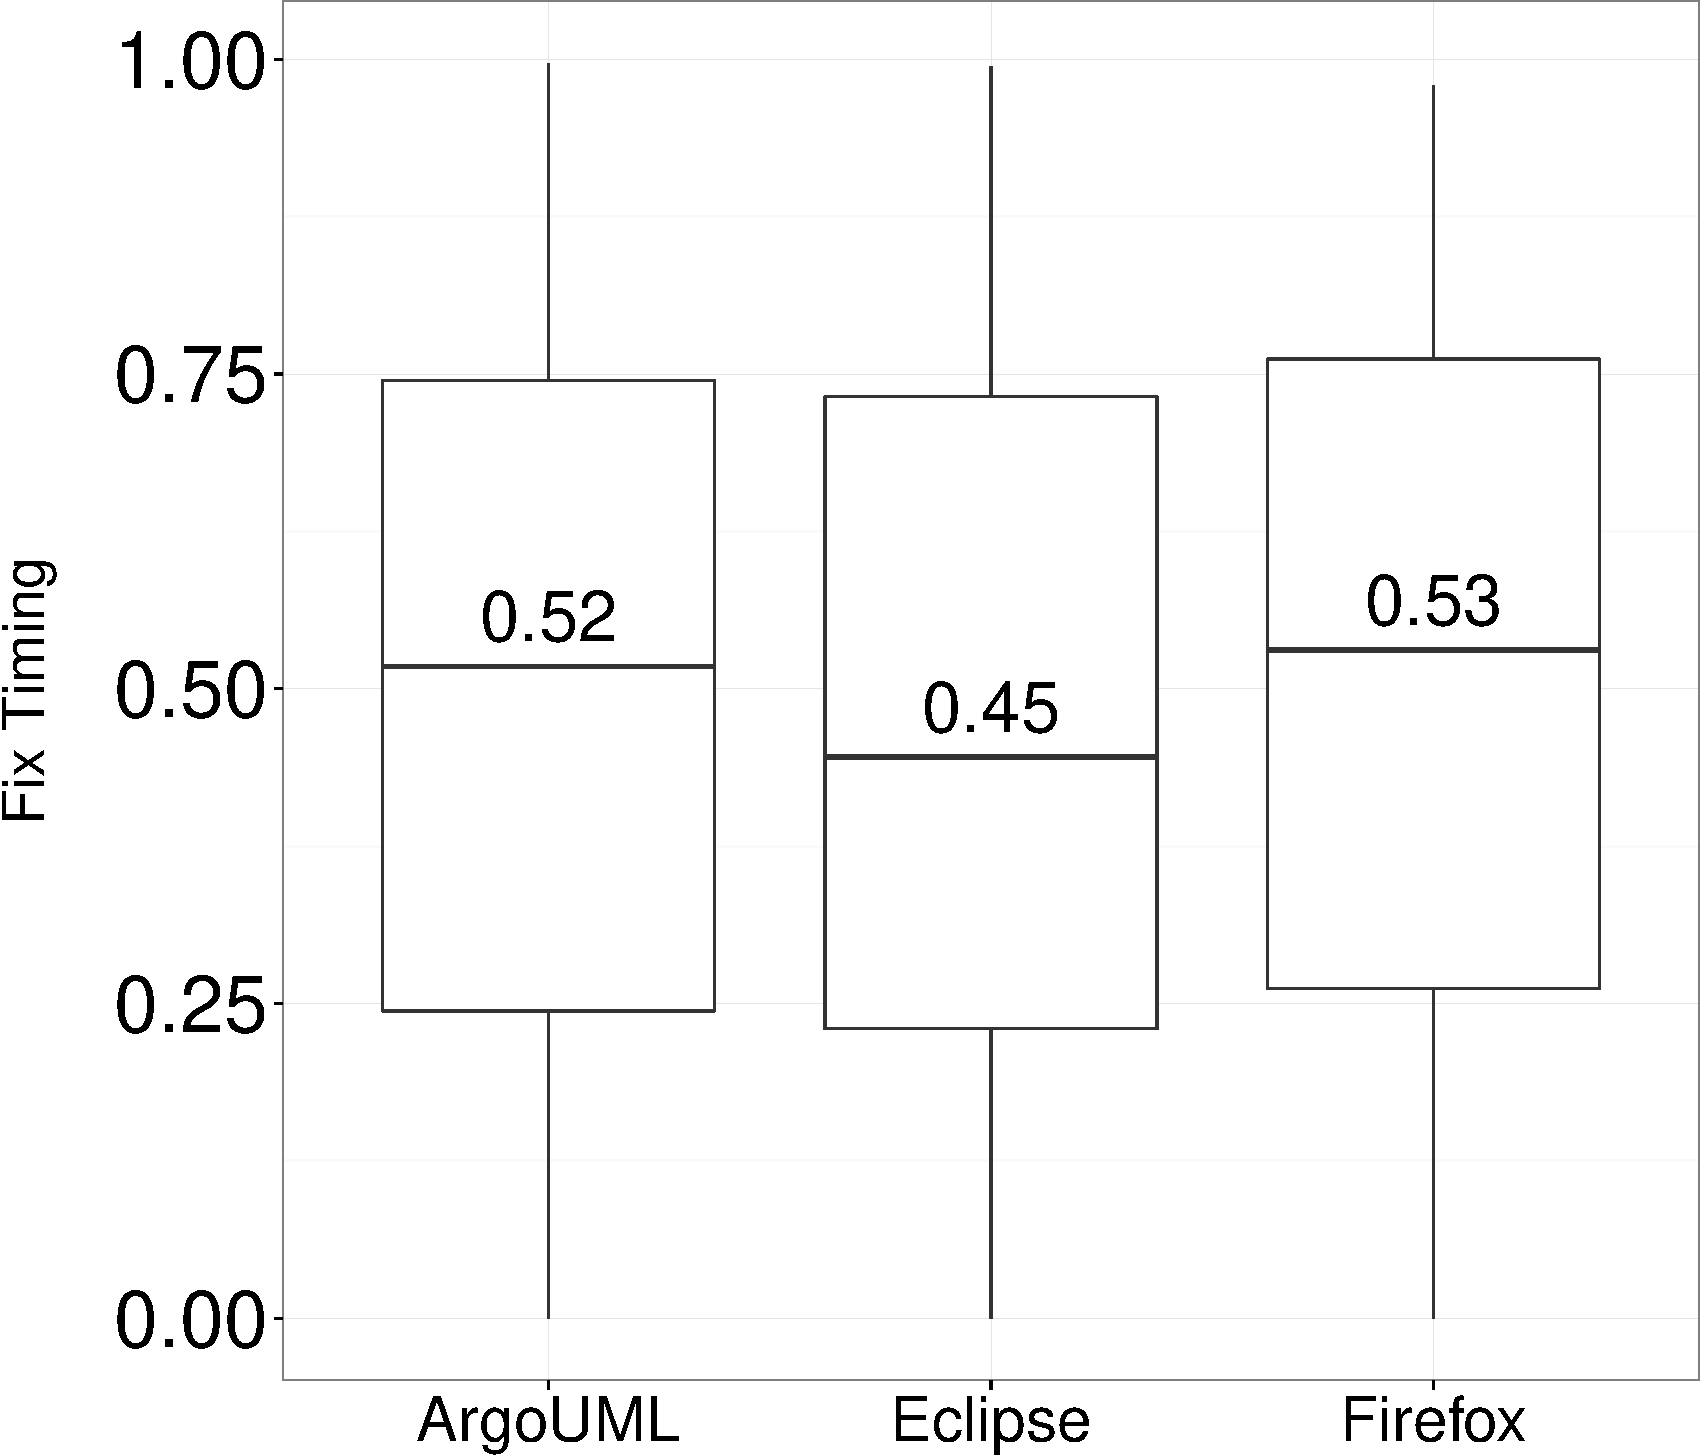
\includegraphics[width=0.7\textwidth]
	{chapters/chapter4/figures/addressing_stage.pdf}
	\caption{\textbf{Fix timing metric.} We present the
		distribution of the \textit{fix timing} metric for addressed
		issues that are prevented from integration in at least one release.}
	\label{ch4:fig:boxplotTimeWindow}
\end{figure}

\noindent\textit{\textbf{Many issues that were prevented from integration are
addressed well before the upcoming release date.}} addressed issues could be prevented
from integration because they were addressed late in the release cycle, \eg one day
or one week before the upcoming release date. To check whether addressed issues are
being prevented from integration mostly because they are being addressed late in the
release cycle, we compute the \textit{fix timing} metric. 

\hyperref[ch4:fig:boxplotTimeWindow]{Figure}~\ref{ch4:fig:boxplotTimeWindow} shows the
distribution of the \textit{fix timing} metric for each project. The smallest
\textit{fix timing} median is observed for the Eclipse project, which is 0.45.
For the ArgoUML and Firefox projects, the median is 0.52 and 0.53, respectively.
The \textit{fix timing} medians are roughly in the middle of the release.
Moreover, the boxes extend to cover between 0.25 and 0.75. The result suggests
that, in the studied projects, issues that are prevented from integration are
usually addressed $\frac{1}{4}$ to $\frac{3}{4}$ of the way through a release.
Hence, it is unlikely that most addressed issues are prevented from integration
solely because they were addressed too close to an upcoming release date.

\conclusionbox{The integration of 34\% to 60\% of the addressed issues in the
	traditionally released projects and 98\% in the rapidly released project
	were prevented from integration in at least one release. Furthermore, we
	find that many issues which integration was prevented, were addressed well
before the releases from which they were omitted.}


\subsection*{\textbf{\textit{RQ2: Does the stage of the release cycle impact delivery delay?}}}

\noindent\textit{\textbf{Issues that are addressed during more stable stages of a
release cycle have a shorter delivery delay.}}
\hyperref[ch4:fig:cycle_phases]{Figure}~\ref{ch4:fig:cycle_phases} shows the
distributions of delivery delay (in terms of days) per each release cycle
stage of the studied projects. For the Eclipse project, the stages are divided
into {\em milestones}, {\em RCs} (Release Candidates), and {\em code freeze}
(see the \hyperref[eclipse:releng]{release engineering} process of Eclipse). Indeed, issues that
are addressed during RCs have a shorter delivery delay when
compared to issues that were addressed during milestone releases. For the difference
between {\em milestones} and {\em RCs}, we observe a $p=1.47 \times 10^{-52}$ and a {\em
large} effect-size of $delta=0.63$. All of the $p$-$values$ and $deltas$ of our
statistical analysis are shown in
\hyperref[ch4:tbl:statisticalrq2]{Table}~\ref{ch4:tbl:statisticalrq2}. Even though
delivery delay seems to be larger during the {\em code freeze} stage, we do
not observe a significant $p$-$value$ when comparing the {\em code freeze} stage
to the other stages. In fact, only ten issues were addressed during the {\em code freeze}
stage in our data, which impairs statistical observations of trends in such a stage.

For the Firefox project, we observe that delivery delay tends to be
shorter as fixes are performed along more stable stages. For example, by
comparing the delivery delay values between the {\em NIGHTLY} and {\em
AURORA} stages, we observe a $p=5.1 \times 10^{-49}$ and a {\em medium}
effect-size of $delta = 0.40$ (the other comparisons are shown in
\hyperref[ch4:tbl:statisticalrq2]{Table}~\ref{ch4:tbl:statisticalrq2}).

Finally, for the ArgoUML project, we also observe a trend of shorter
delivery delay as the fixes are performed during more stable stages of release
cycles. For instance, when we compare the delivery delay of addressed issues of the {\em alpha}
and {\em beta} stages, we obtain a $p$-$value$ of $3.98 \times 10^{-09}$ and a {\em
large} effect-size of $delta = 0.98$.\\

\begin{figure}
	\centering
	\subfloat[Eclipse]{
		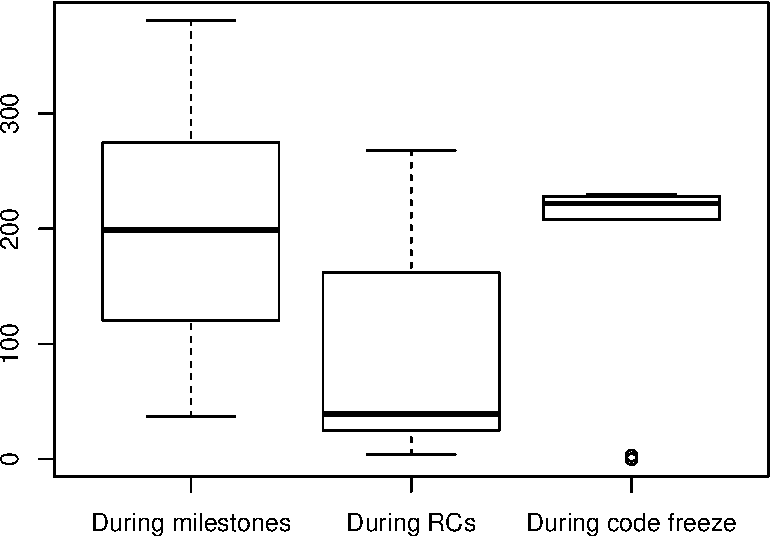
\includegraphics[width=0.60\textwidth,keepaspectratio]
		{chapters/chapter4/figures/eclipse_phases_boxplot.pdf}
	}

	\subfloat[Firefox]{
		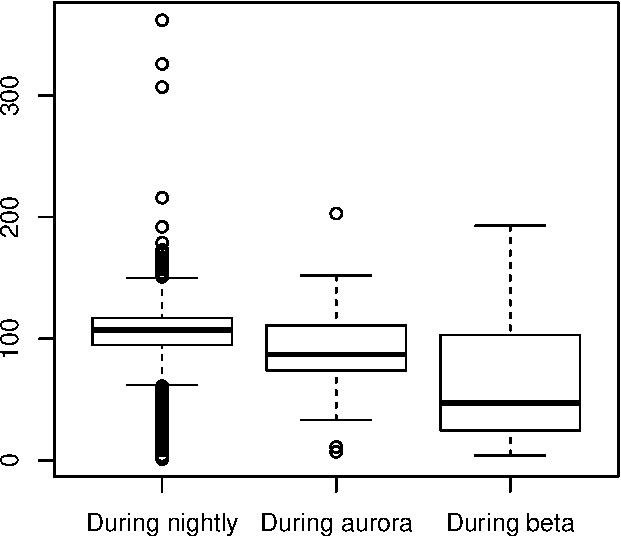
\includegraphics[width=0.60\textwidth,keepaspectratio]
		{chapters/chapter4/figures/firefox_phases_boxplot.pdf}
	}

	\subfloat[ArgoUML]{
		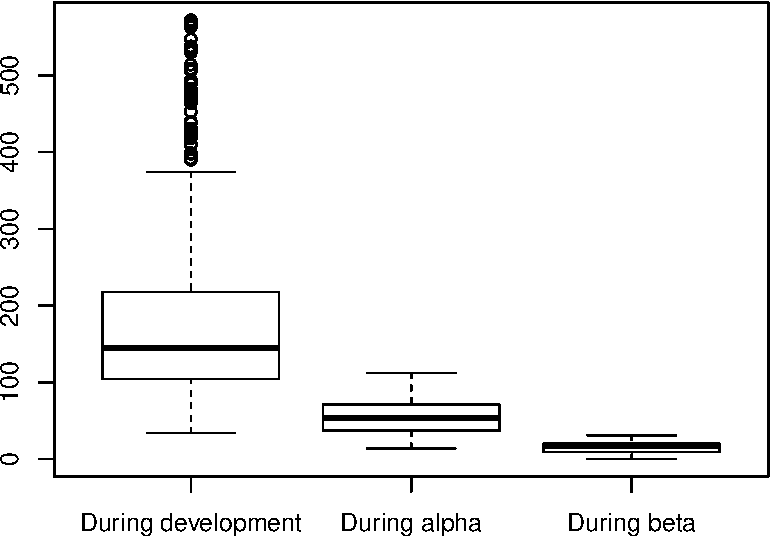
\includegraphics[width=0.60\textwidth,keepaspectratio]
		{chapters/chapter4/figures/argouml_phases_boxplot.pdf}
	}

	\caption{\textbf{delivery delay during release
		cycle stages.} Issues that are addressed during more stable stages of a release cycle
	are likely to have a shorter delivery delay}
	\label{ch4:fig:cycle_phases}
\end{figure}


\begin{table}
	\footnotesize
	\centering
	\caption{\textbf{Statistical analysis.} An overview of the $p$-$values$
		and $deltas$ that are observed during our statistical analyses.
		\label{ch4:tbl:statisticalrq2}
	}
	\resizebox{\textwidth}{!}{
		\begin{tabular}{llrrr}
			\hline 
			& \textbf{Comparison} & \textbf{Kruskal-Wallis} ($p$) &
			\textbf{Dunn} ($p.adjusted$) & \textbf{Effect-size} ($delta$)\tabularnewline
			\hline 
			\multirow{3}{*}{\textbf{Eclipse}} & Milestones vs RCs &
			\multirow{3}{*}{$1.87 \times 10^{-51}$} & $1.47 \times 10^{-52}$ & (large) $0.63$\tabularnewline
			\cline{2-2} \cline{4-5} & RCs vs Code freeze &  & $0.56$ & Not apply\tabularnewline \cline{2-2} \cline{4-5} & Milestones vs Code freeze &  & $0.02$ & (negligible) $0.09$\tabularnewline
			\hline 
			\multirow{3}{*}{\textbf{Firefox}} & Nightly vs Aurora &
			\multirow{3}{*}{$2.99 \times 10^{-76}$} & $5.07 \times 10^{-49}$ &
			(medium) $0.40$\tabularnewline
			\cline{2-2} \cline{4-5} 
			& Aurora vs Beta &  & $1.72 \times 10^{-03}$ & (medium) $0.40$\tabularnewline
			\cline{2-2} \cline{4-5} 
			& Nightly vs Beta &  & $1.43 \times 10^{-31}$ & (large) $0.57$\tabularnewline
			\hline 
			\multirow{3}{*}{\textbf{ArgoUML}} & Development vs Alpha
			& \multirow{3}{*}{$2.73 \times 10^{-135}$} & $7.24 \times 10^{-89}$
			& (large) $0.94$\tabularnewline
			\cline{2-2} \cline{4-5} 
			& Alpha vs Beta &  & $3.98 \times 10^{-09}$ & (large) $0.98$\tabularnewline
			\cline{2-2} \cline{4-5} 
			& Development vs Beta &  & $1.14 \times 10^{-78}$ & (large) $0.99$\tabularnewline
			\hline 
		\end{tabular}
	}
\end{table}

\noindent\textit{\textbf{Many issues that are prevented from integration are
addressed well before the code freeze stage of their respective release cycle.}} We
compute the {\em fix timing} metric that we present in \hyperref[rq1]{RQ1}.
However, instead of counting the number of days until an upcoming release, we
count the number of days until an upcoming code freeze stage
(\hyperref[ch4:eq:fixtiming2]{Equation}~\ref{ch4:eq:fixtiming2}). Our goal is to check
whether addressed issues are being prevented from integration mostly because they
are being addressed too close to a code freeze stage (\ie a period during which
integration of new code changes would likely be minimal).  

\begin{figure} \center 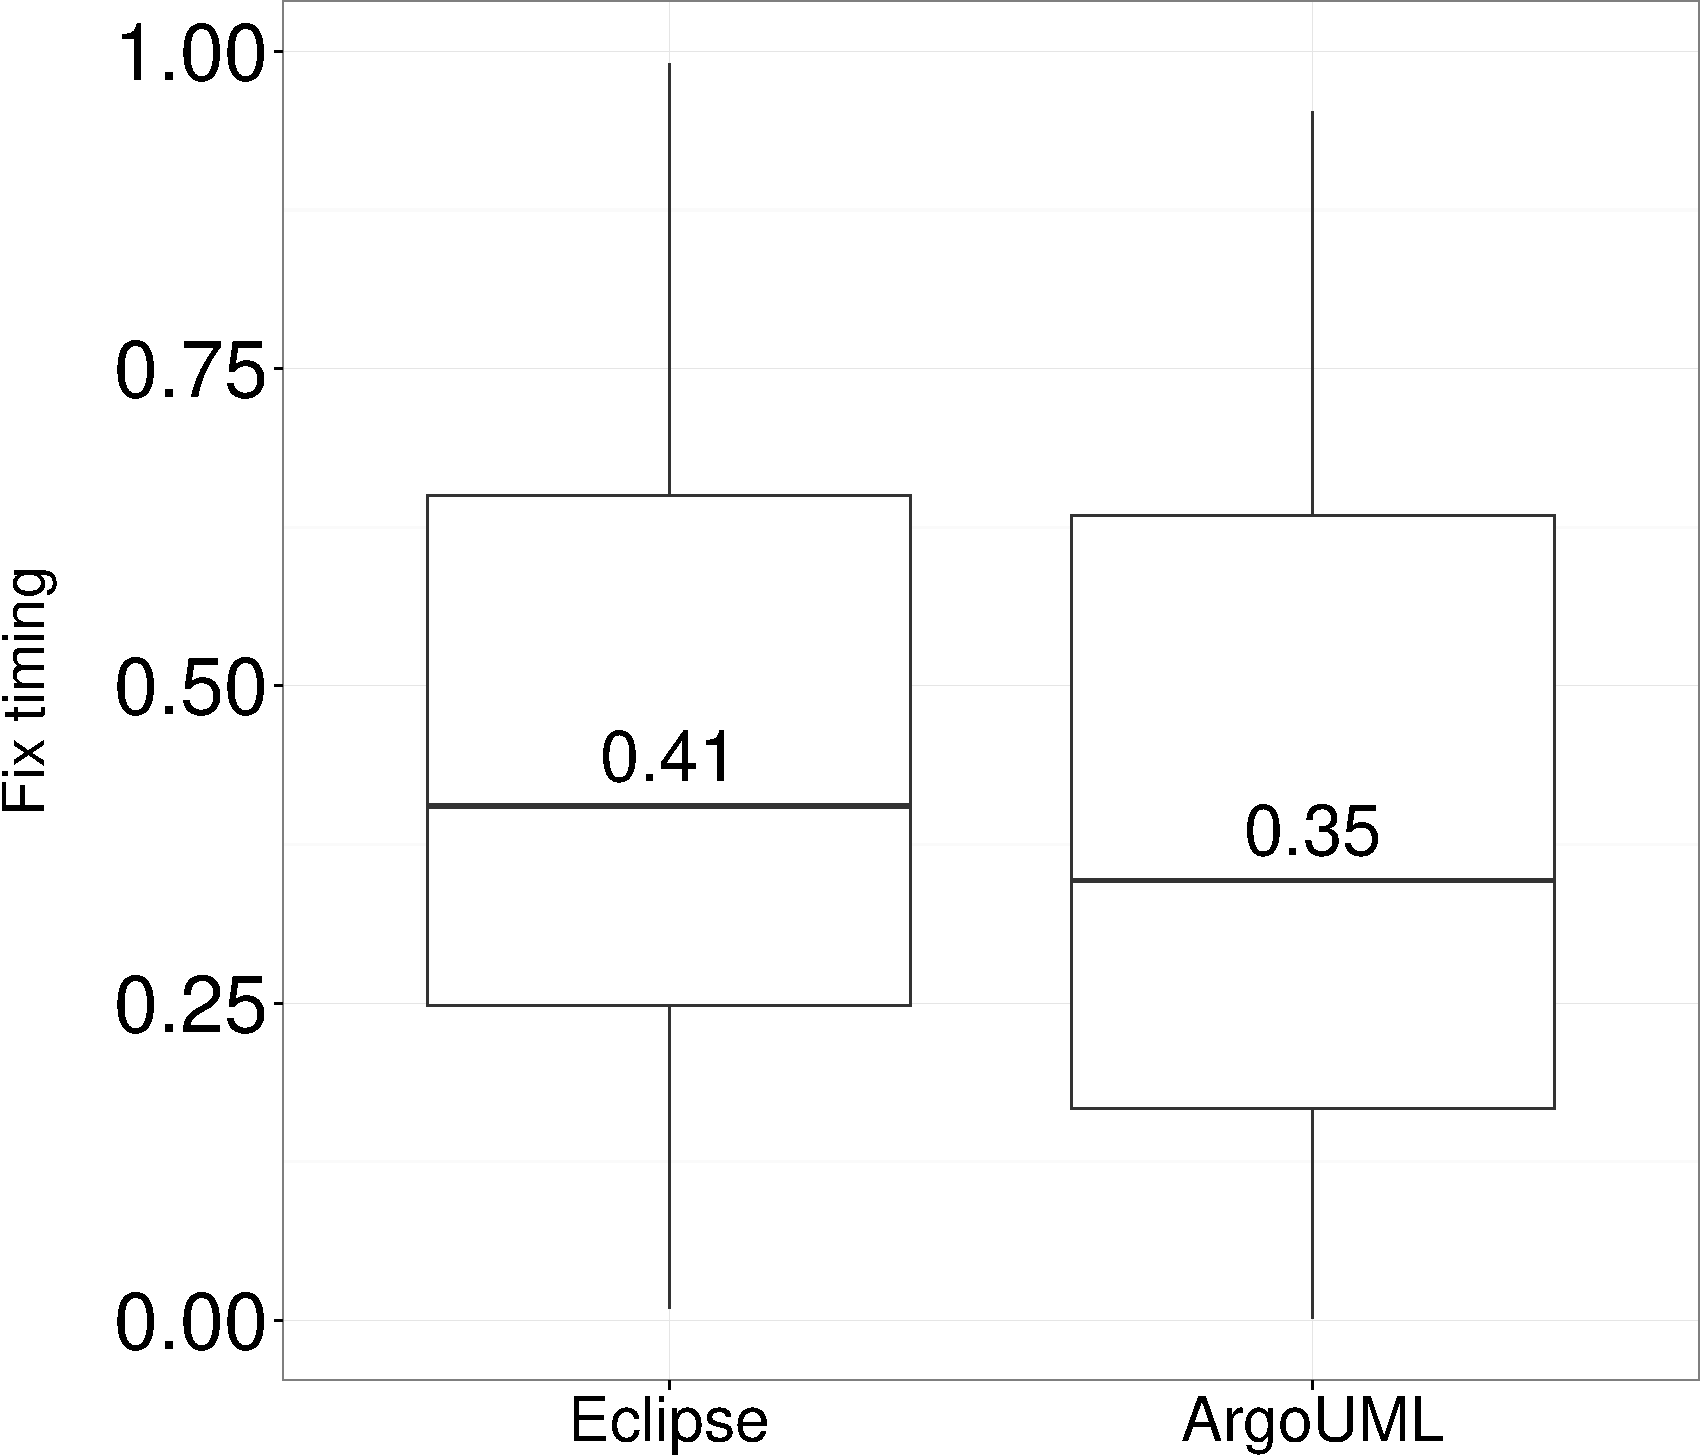
\includegraphics[width=0.60\textwidth,keepaspectratio]
	{chapters/chapter4/figures/as_codefreeze.pdf} \caption{\textbf{{\em Fix timing} values for
		the code freeze period.} The median {\em fix timing} values drop
		from 0.45 and 0.52 to 0.41 and 0.35 in the Eclipse and ArgoUML
projects, respectively. } \label{ch4:fig:codefreeze_allsystems} \end{figure}

In \hyperref[ch4:fig:codefreeze_allsystems]{Figure}~\ref{ch4:fig:codefreeze_allsystems},
we show the {\em fix timing} values for the Eclipse and ArgoUML projects, since
both projects adopt a {\em code freeze} stage. For the Eclipse project, the code
freeze starts after the last release candidate, while for the ArgoUML project,
the code freeze starts at the beginning of the {\em beta} stage (see
\hyperref[ch4:sec:subjects]{Section}~\ref{ch4:sec:subjects}). Naturally, we observe a
drop in the {\em fix timing} values, since both code freeze stages start considerably
before the official release dates. Nevertheless, we observe that even after correcting for
the code freeze stages of the Eclipse and ArgoUML projects, it is unlikely
that addressed issues are being prevented from integration solely because of an approaching code
freeze stage. For instance, although the median {\em fix timing} for the ArgoUML project
dropped from 0.52 to 0.35, the development team would still have 2 months to
integrate an addressed issue---since the median duration of a release cycle in the
ArgoUML project is 180 days.

\conclusionbox{We observe that issues that are addressed during more stable stages of
release cycles are associated with a shorter delivery delay. We also observe
that addressed issues are unlikely to be prevented from integration solely because
they were addressed near an upcoming code freeze stage.}


\subsection*{\textbf{\textit{RQ3: How well can we model the delivery delay of addressed issues?}}}

\begin{figure}
	\centering
	%\captionsetup{justification=centering}
	\subfloat[Eclipse]{
		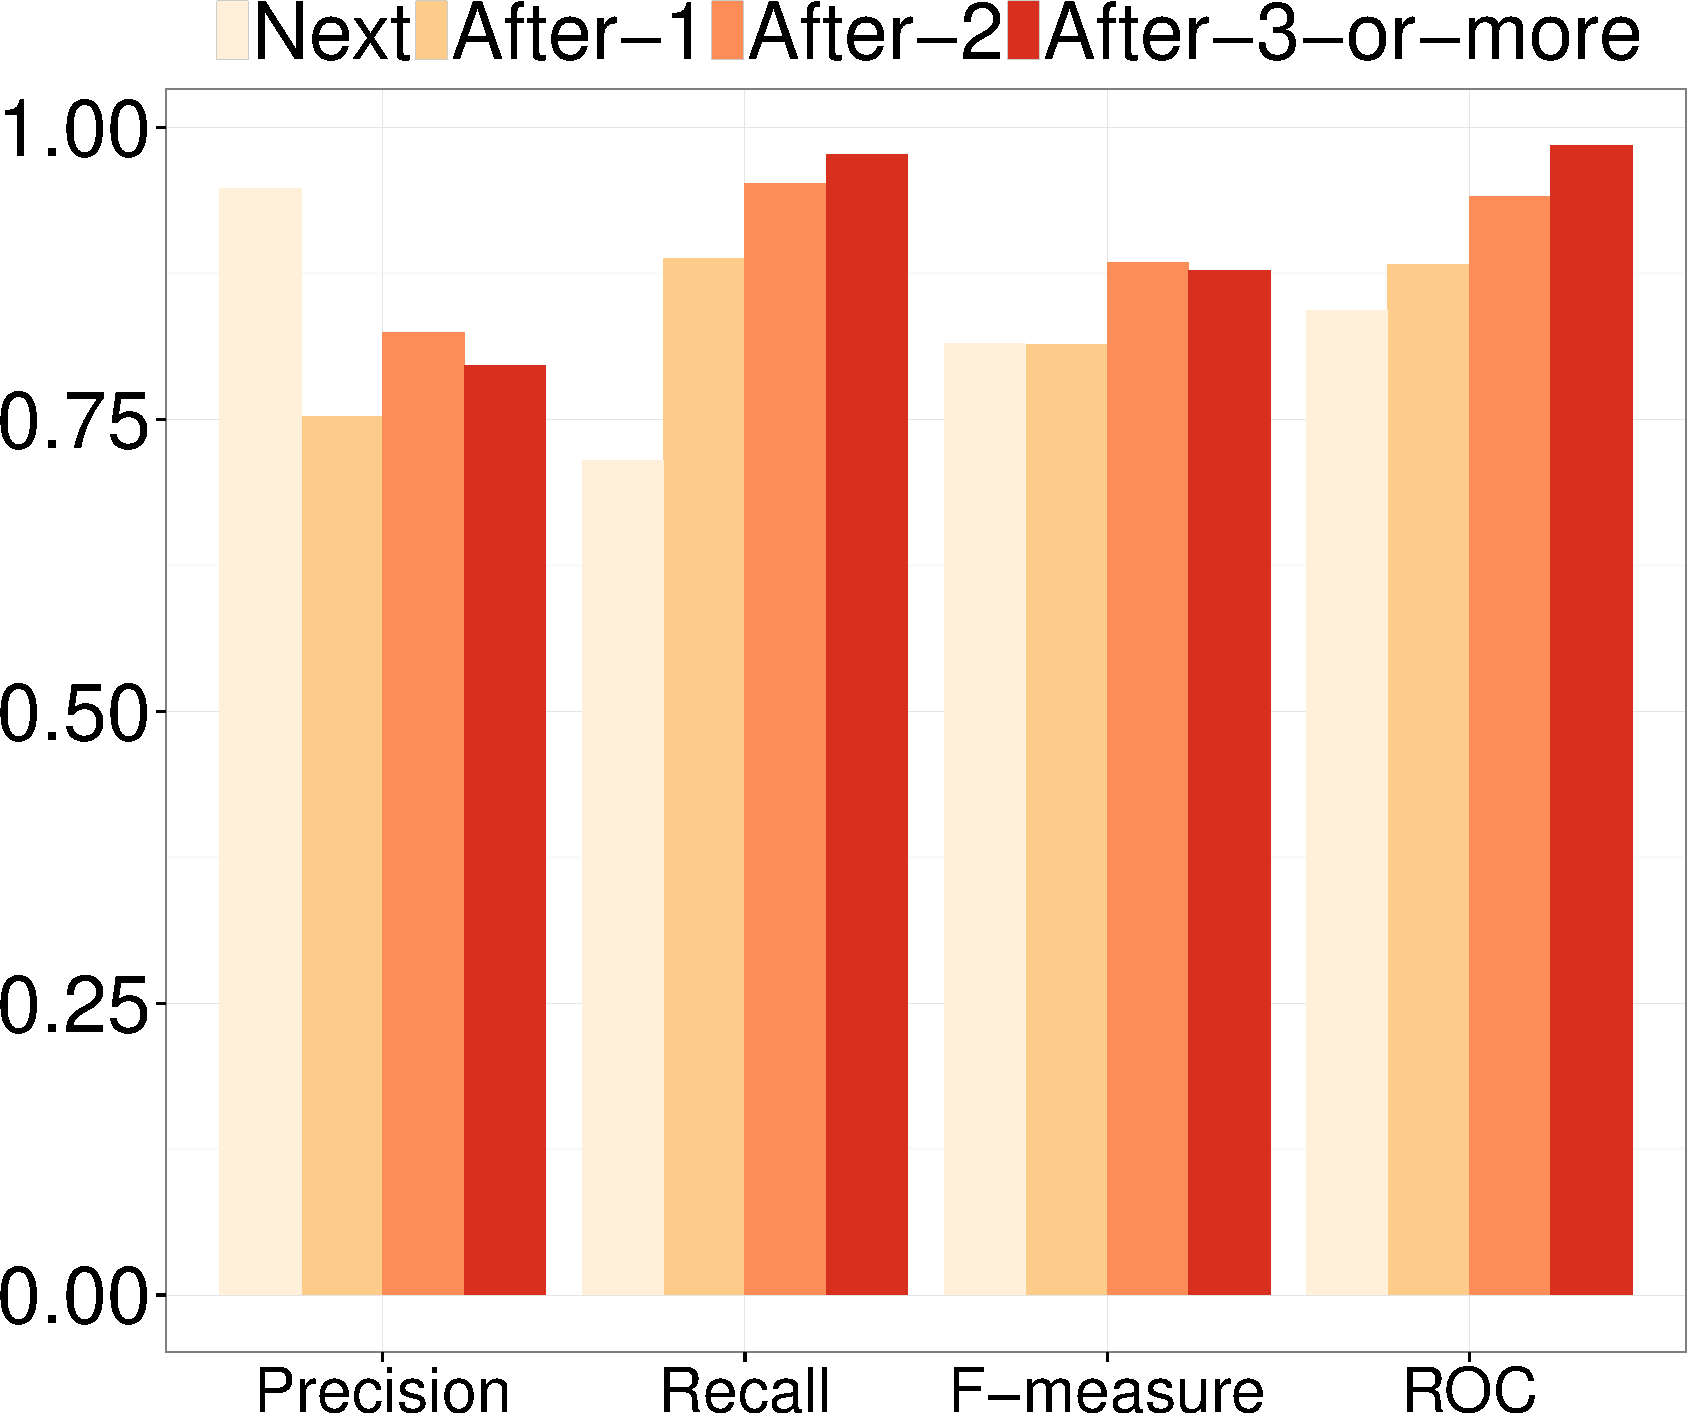
\includegraphics[width=0.50\textwidth,keepaspectratio] 
		{chapters/chapter4/figures/eclipse_loocv_evaluation.pdf}
		\label{ch4:fig:RFeclipse}
	}

	\subfloat[Firefox]{
		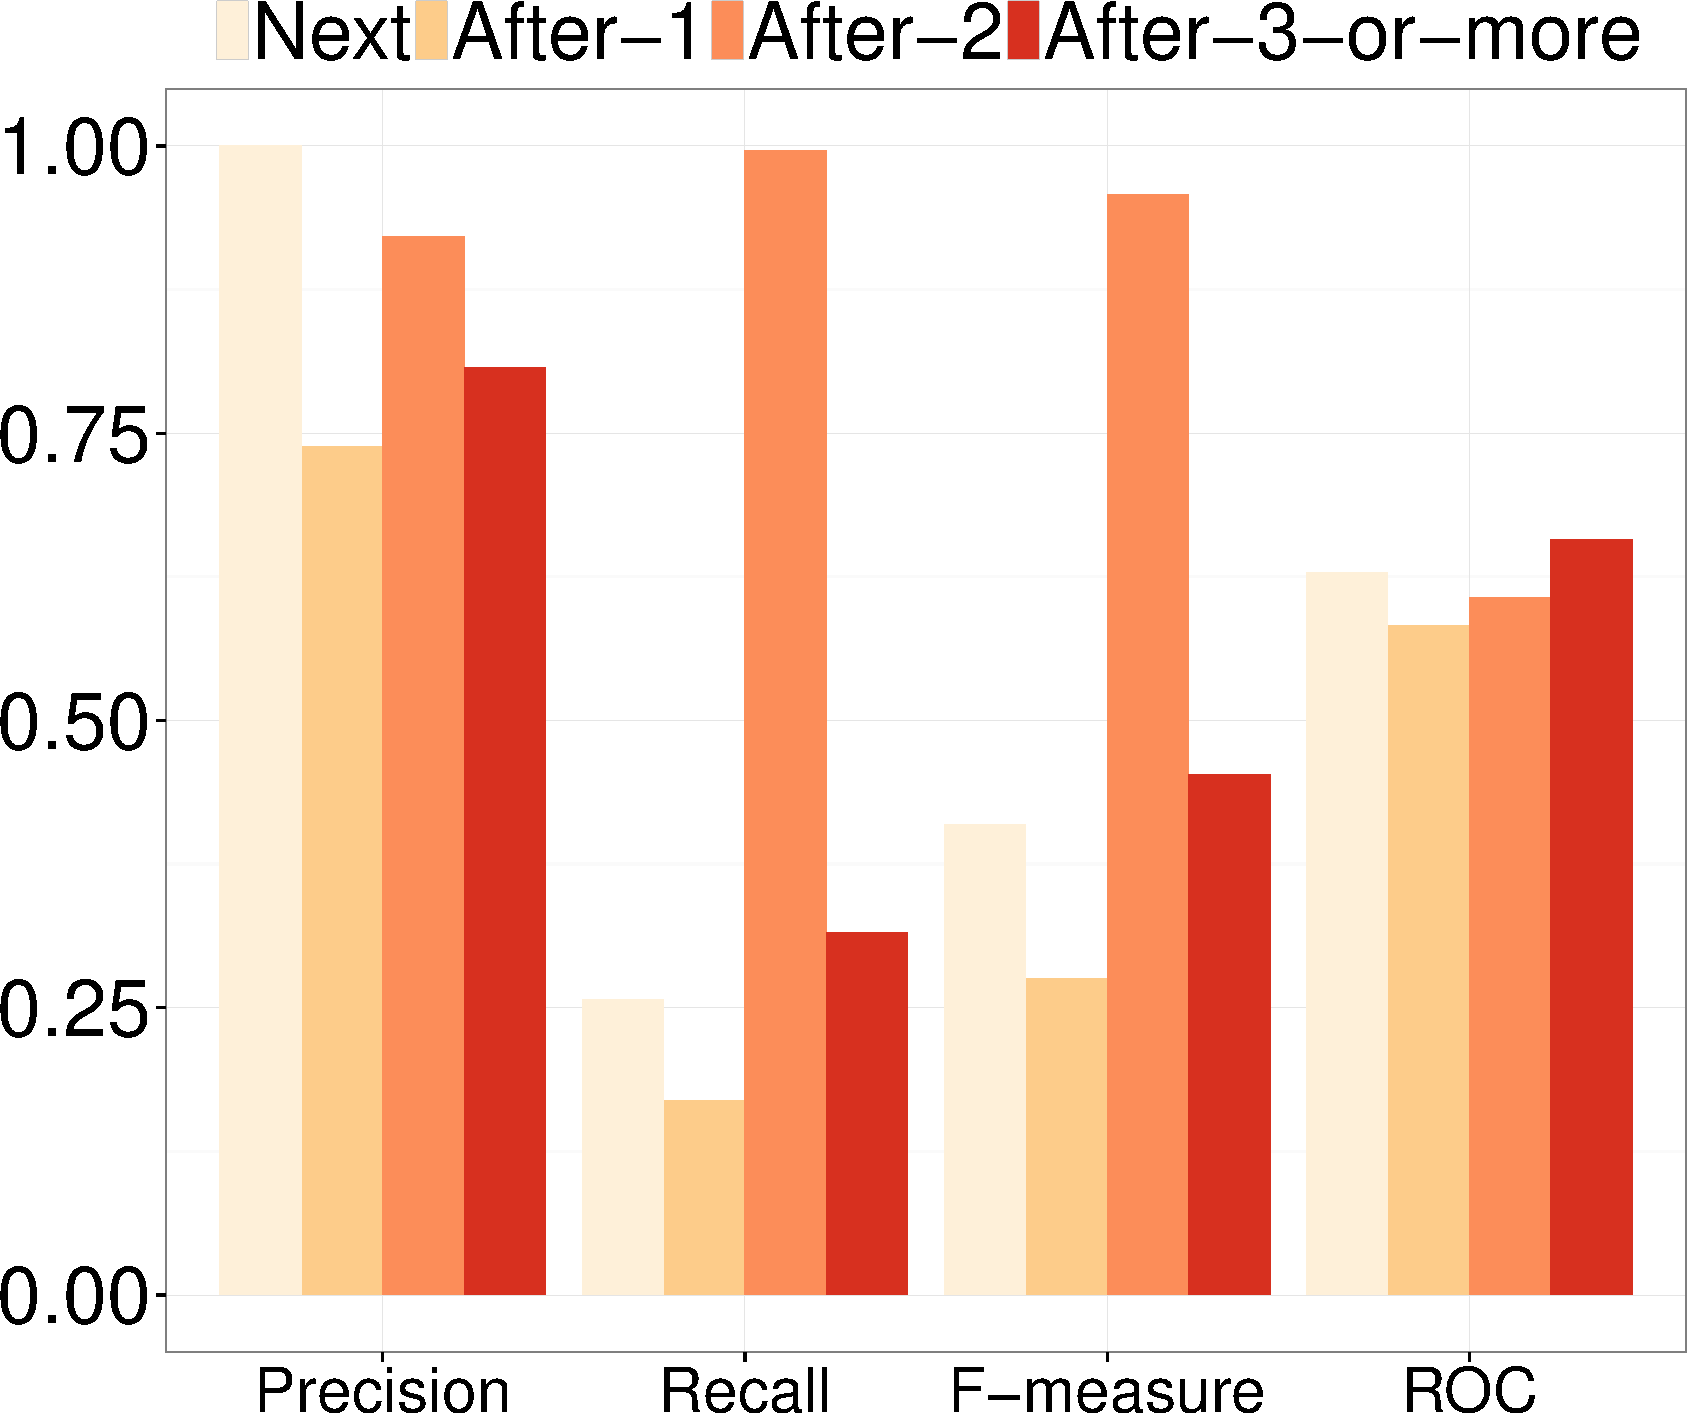
\includegraphics[width=0.50\textwidth,keepaspectratio]  
		{chapters/chapter4/figures/firefox_loocv_evaluation.pdf}
		\label{ch4:fig:RFfirefox}
	}

	\subfloat[ArgoUML]{
		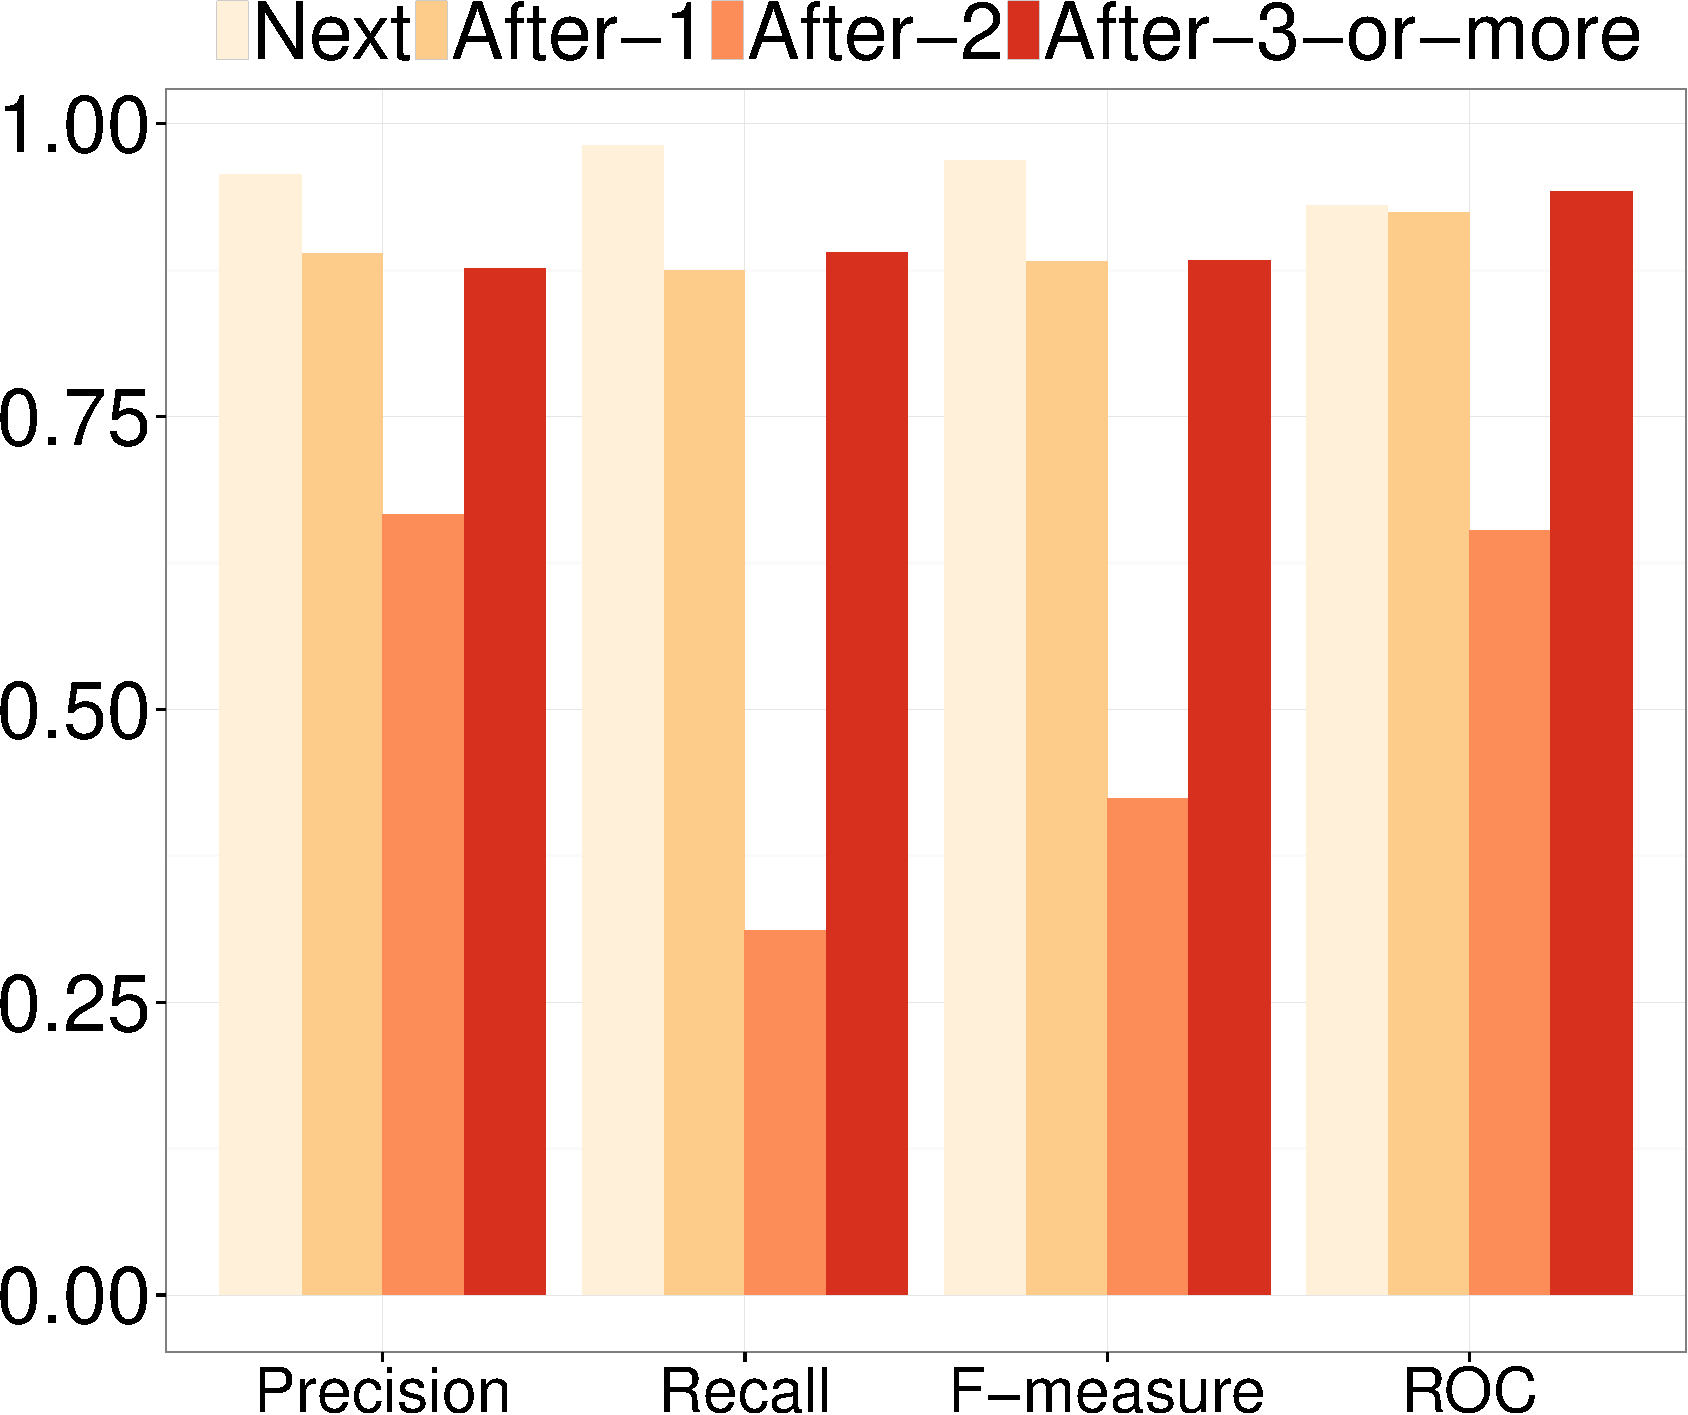
\includegraphics[width=0.50\textwidth,keepaspectratio] 
		{chapters/chapter4/figures/argouml_loocv_evaluation.pdf}
		\label{ch4:fig:RFargo}
	}
	\caption{\textbf{Performance of random forest models.} We show the
	values of Precision, Recall, F-measure, and AUC that are
computed using the LOOCV technique.}
	\label{ch4:fig:RFclassificationResult}
\end{figure}

\begin{table}
	\footnotesize
	\centering
	\caption{The precision, recall, F-measure, and AUC values that are
	obtained for the Eclipse, Firefox, and ArgoUML projects. 
	\label{ch4:tbl:evaluation_metrics}
	}
	\begin{tabular}{lcccc}
		\hline
		\multicolumn{5}{c}{\textbf{Eclipse}}\tabularnewline
		\hline 
		\textbf{Bucket} & \textbf{Precision} & \textbf{Recall} &
		\textbf{F-measure} & \textbf{AUC}\tabularnewline
		\hline 
		Next & 0.95  & 0.71  & 0.81 & 0.84 \tabularnewline
		\hline 
		After-1 & 0.75 & 0.89 & 0.81 & 0.88\tabularnewline
		\hline 
		After-2 & 0.82 & 0.95 & 0.88 & 0.94\tabularnewline
		\hline 
		After-3-or-more & 0.80 & 0.98 & 0.88 & 0.98\tabularnewline
		\hline 
		\hline
		\multicolumn{5}{c}{\textbf{Firefox}}\tabularnewline
		\hline 
		\textbf{Bucket} & \textbf{Precision} & \textbf{Recall} &
		\textbf{F-measure} & \textbf{AUC}\tabularnewline
		\hline 
		Next & 0.99  & 0.26  & 0.41 & 0.63 \tabularnewline
		\hline 
		After-1 & 0.74 & 0.17 & 0.28 & 0.58\tabularnewline
		\hline 
		After-2 & 0.92 & 0.99 & 0.96 & 0.61\tabularnewline
		\hline 
		After-3-or-more & 0.81 & 0.32 & 0.45 & 0.66\tabularnewline
		\hline 
		\hline
		\multicolumn{5}{c}{\textbf{ArgoUML}}\tabularnewline
		\hline 
		\textbf{Bucket} & \textbf{Precision} & \textbf{Recall} &
		\textbf{F-measure} & \textbf{AUC}\tabularnewline
		\hline 
		Next & 0.96  & 0.98  & 0.97 & 0.93 \tabularnewline
		\hline 
		After-1 & 0.89 & 0.87 & 0.88 & 0.92\tabularnewline
		\hline 
		After-2 & 0.67 & 0.31 & 0.42 & 0.65\tabularnewline
		\hline 
		After-3-or-more & 0.88 & 0.89 & 0.88 & 0.94\tabularnewline
		\hline 
	\end{tabular}
\end{table}

\subsubsection*{\textit{\textbf{RQ3: Results for delivery delay in terms of
releases}}}

\noindent\textit{\textbf{Our explanatory models obtain a median precision of 0.81 to
0.88 and a median recall of 0.29 to 0.92.}}
\hyperref[ch4:fig:RFclassificationResult]{Figure}~\ref{ch4:fig:RFclassificationResult}
shows the precision, recall, F-measure, and AUC of our explanatory models.  The
bar charts show the values that we observe for each bucket. The values of
precision, recall, F-measure, and AUC are also shown in
\hyperref[ch4:tbl:evaluation_metrics]{Table}~\ref{ch4:tbl:evaluation_metrics}. 

The best precision/recall values that we obtain for the Eclipse, Firefox, and
ArgoUML projects are related to the \textit{after-2} (F-measure of 0.88),
\textit{after-2} (F-measure of 0.96), and \textit{next} (F-measure of 0.97),
respectively. However, for buckets with low number of instances,
precision/recall values decrease considerably. For instance, the F-measures that
are obtained by our models for the Firefox project are considerably low for the
\textit{next}, \textit{after-1}, and \textit{after-3-or-more} buckets (0.41,
0.28 and 0.45, respectively).

Moreover, our models obtain median AUCs between 0.62 to 0.96, which indicate
that our model estimations are better than random guessing (AUC of 0.5).
Summarizing the results, our models obtain a median precision of 0.81-0.88
(median) and a median recall of 0.29-0.92. Our models provide a sound starting
point for studying the release into which an addressed issue will be integrated.\\

\noindent\textit{\textbf{Our models obtain better F-measure values than
Zero-R.}} We compared our models to Zero-R models as a baseline. For all test
instances, Zero-R selects the bucket that contains the majority of the instances.
Hence, the recall for the bucket containing the majority of instances is 1.0. We
compared the F-measure of our models to the F-measure of Zero-R models. We
choose to compare to the F-measure values because precision and recall are very
skewed for Zero-R. 

For the Firefox project, Zero-R obtains an F-measure of 0.95 for the
\textit{after-2} bucket, whereas our model obtains an F-measure of 0.96 for the
same bucket. For the Eclipse project, Zero-R always selects \textit{next} and
obtains a F-measure of 0.58, while our model obtains an F-measure of 0.81.
Finally, for the ArgoUML project, Zero-R always selects \textit{next} with an
F-measure of 0.84, whereas our model obtains an F-measure of 0.97. These results
show that our models yield better F-measure values than na\"{i}ve techniques
like Zero-R or random guessing (AUC = 0.5) in the majority of cases.  

\conclusionbox{We are able to accurately model how many releases an addressed issue
is likely to be prevented from integration. Our models outperform na\"{i}ve
techniques, such as Zero-R and random guessing, obtaining AUC values of 0.62 to
0.96.}

\begin{table}
	\centering
	\footnotesize
	\caption{\textbf{Regression results of model fit.} Our explanatory
		models obtain $R^2$ values between 0.39 to 0.65 and MAE values between
	7.8 to 66 days.}
	\label{ch4:tbl:regression_results}
	\def\arraystretch{1.5}
	\begin{tabular}{lrrr}
		\hline 
		\centering{\textbf{Metric/Project}} &
		\centering{\textbf{Eclipse}} & \centering{\textbf{Firefox}} &
		\centering{\textbf{ArgoUML}} \tabularnewline
		\hline 
		$R^2$ & 0.48  & 0.39 & 0.65 \tabularnewline
		\hline 
		MAE (days) & 61 & 7.8  & 66 \tabularnewline
		\hline 
		Release cycle duration (median in days) & 112 & 42 & 180 \tabularnewline
		\hline
		Error ratio $(\frac{MAE}{cycle})$ & 0.54  & 0.18  & 0.37 \tabularnewline
		\hline 
		Optimism & 0.0267 & 0.0162 & 0.0035 \tabularnewline
		\hline 
	\end{tabular}
\end{table}

\subsubsection*{\textit{\textbf{RQ3: Results for delivery delay in terms of days}}}

\noindent\textbf{\textit{Our explanatory models obtain $R^2$ values of 0.39-0.65
and MAE values between 7.8 to 67 days.}} Our models obtain fair $R^2$ values to
model the variability of delivery delay in days in the studied projects.
\hyperref[ch4:tbl:regression_results]{Table}~\ref{ch4:tbl:regression_results} shows the
$R^2$ and MAE values that are obtained by each of our regression models. The
$R^2$ values for the Eclipse, Firefox, and ArgoUML projects are of 0.39, 0.48,
and 0.65, respectively. 
Additionally, our regression models can provide fair
estimations of delivery delay in days, specially for the Firefox project. For
instance, the median interval in days between releases of the Firefox project is
42 days
(see~\hyperref[ch4:fig:releaseIntervals]{Figure}~\ref{ch4:fig:releaseIntervals}), while
the MAE value for the Firefox project is 7.8 days, which equates to an error
ratio of 18\% (see
\hyperref[ch4:tbl:regression_results]{Table}~\ref{ch4:tbl:regression_results}).\\

\noindent\textbf{\textit{Our explanatory models obtain a good stability with bootstrap
calculated optimism between 0.0035 to 0.0267 of the $R^2$ values.}} We also
observe that our regression models are stable.
\hyperref[ch4:tbl:regression_results]{Table}~\ref{ch4:tbl:regression_results} shows the
\textit{bootstrap-calculated} optimism of the $R^2$ values of our models. The
optimism for the Eclipse, Firefox and ArgoUML projects are 0.0267, 0.0162, and 0.0035,
respectively. Such results indicate that our explanatory models are unlikely to
be overfitted to our data and that our models are stable enough for us to perform the
statistical inferences that follow. 

\conclusionbox{We are able to accurately estimate the delivery delay in terms
of number of days. Our models obtain fair $R^2$ values of 0.39 to 0.65. Our
exploratory models are quite stable with a maximum optimism of 0.0267.}


\subsection*{\textit{\textbf{RQ4: What are the most influential attributes for
modeling delivery delay?}}}

\subsubsection*{\textit{\textbf{RQ4: Results for delivery delay in terms of
releases}}}

\noindent\textit{\textbf{The fixing time per resolver and integration workload
attributes are the most influential attributes in our models.}}
\hyperref[ch4:fig:variableImportance]{Figure}~\ref{ch4:fig:variableImportance} shows the
variable importance values of the LOOCV of our models. The most influential
attribute is the \textit{fixing time per resolver}. The \textit{fixing time per
resolver} attribute measures the total time that is spent by each resolver on
fixing issues in a release cycle. The second most influential attributes are
integration workload attributes (\ie backlog of issues and backlog of issues per
resolver). These integration workload attributes measure the competition of
issues that were addressed but not yet integrated into an official release.

\begin{figure}
	\center
	\subfloat[Eclipse]{
		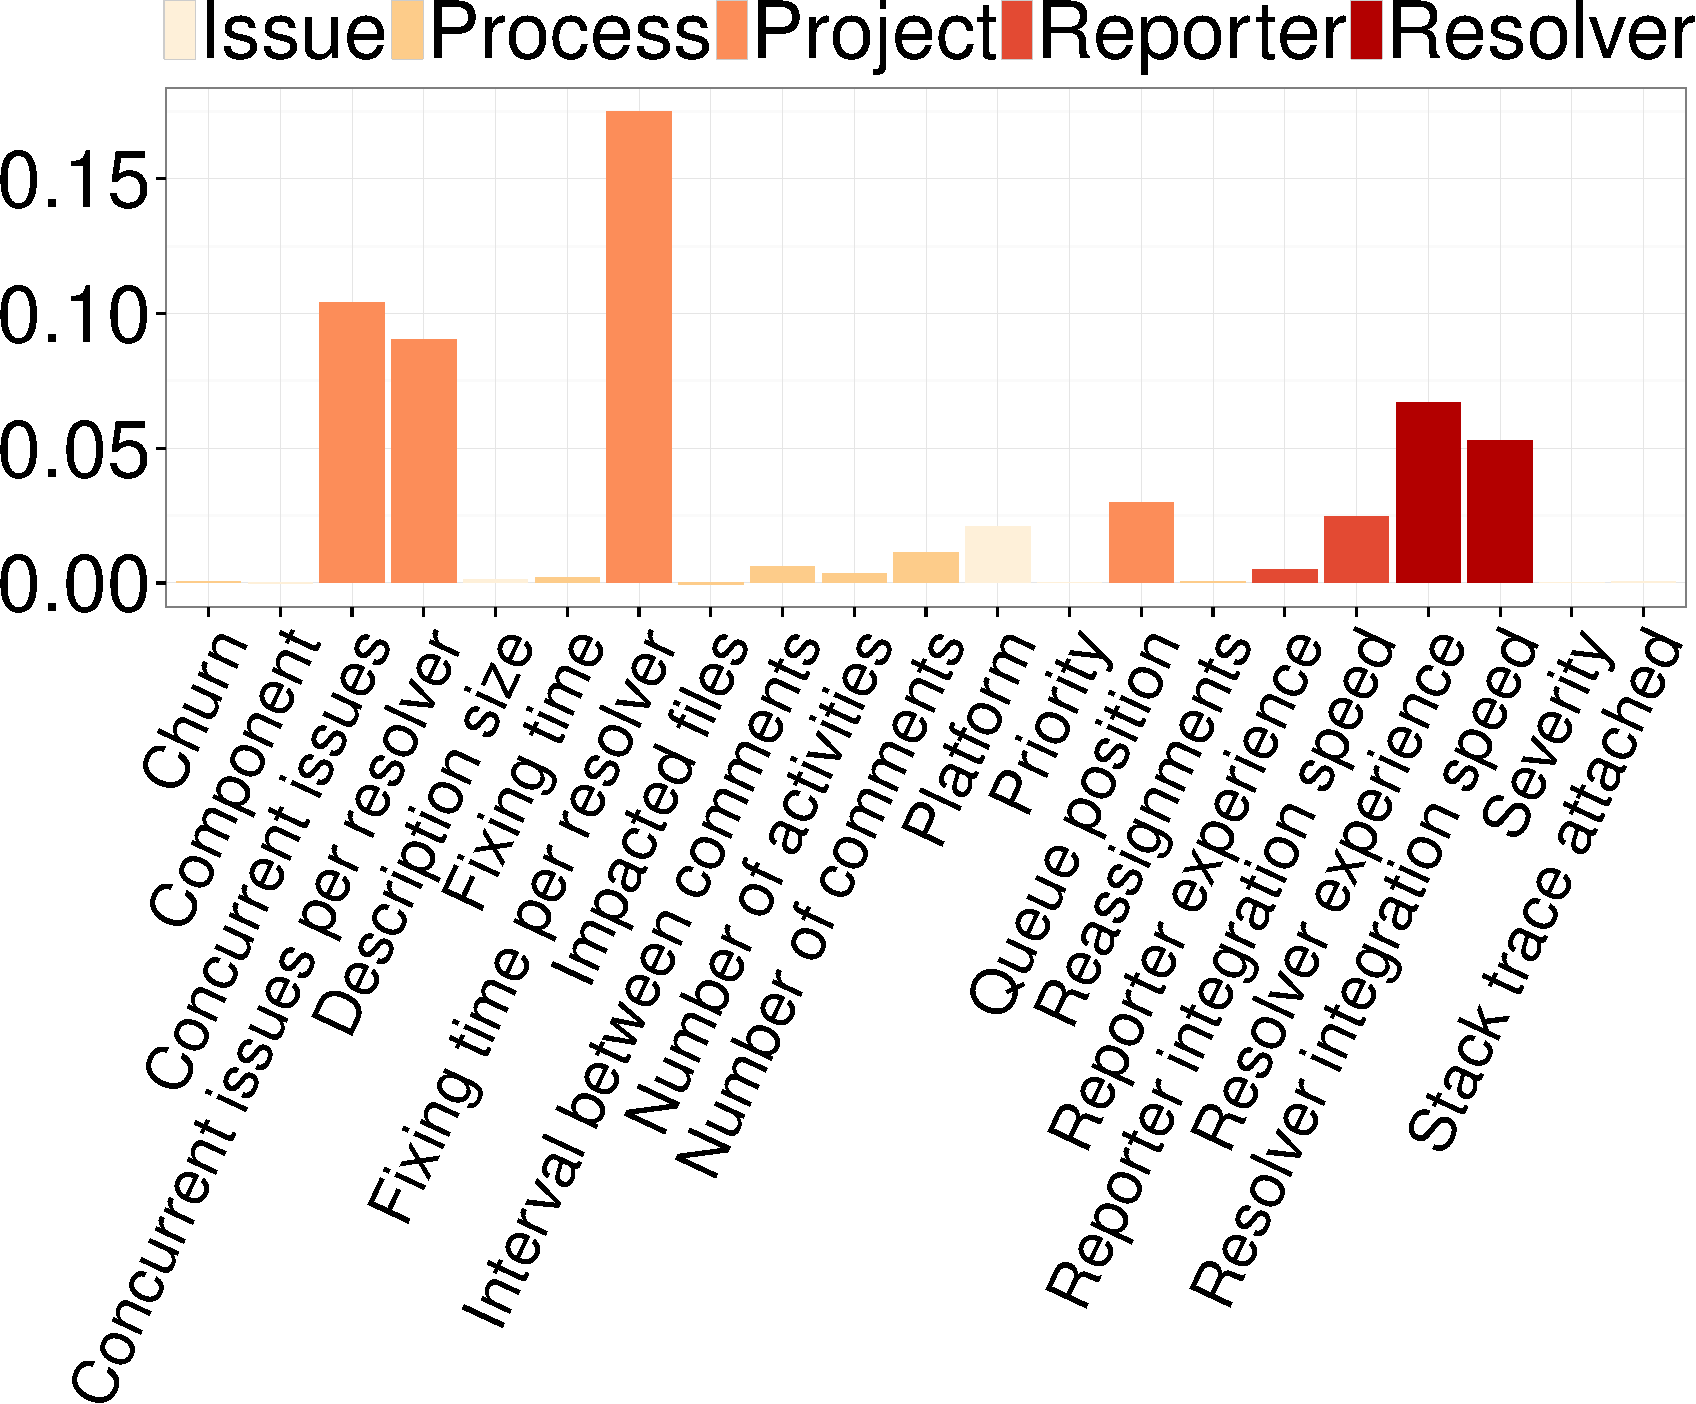
\includegraphics[width=0.55\textwidth,keepaspectratio] 
		{chapters/chapter4/figures/eclipse_loocv_varimp.pdf}
	\label{ch4:fig:impEclipse}
	}

	\subfloat[Firefox]{
		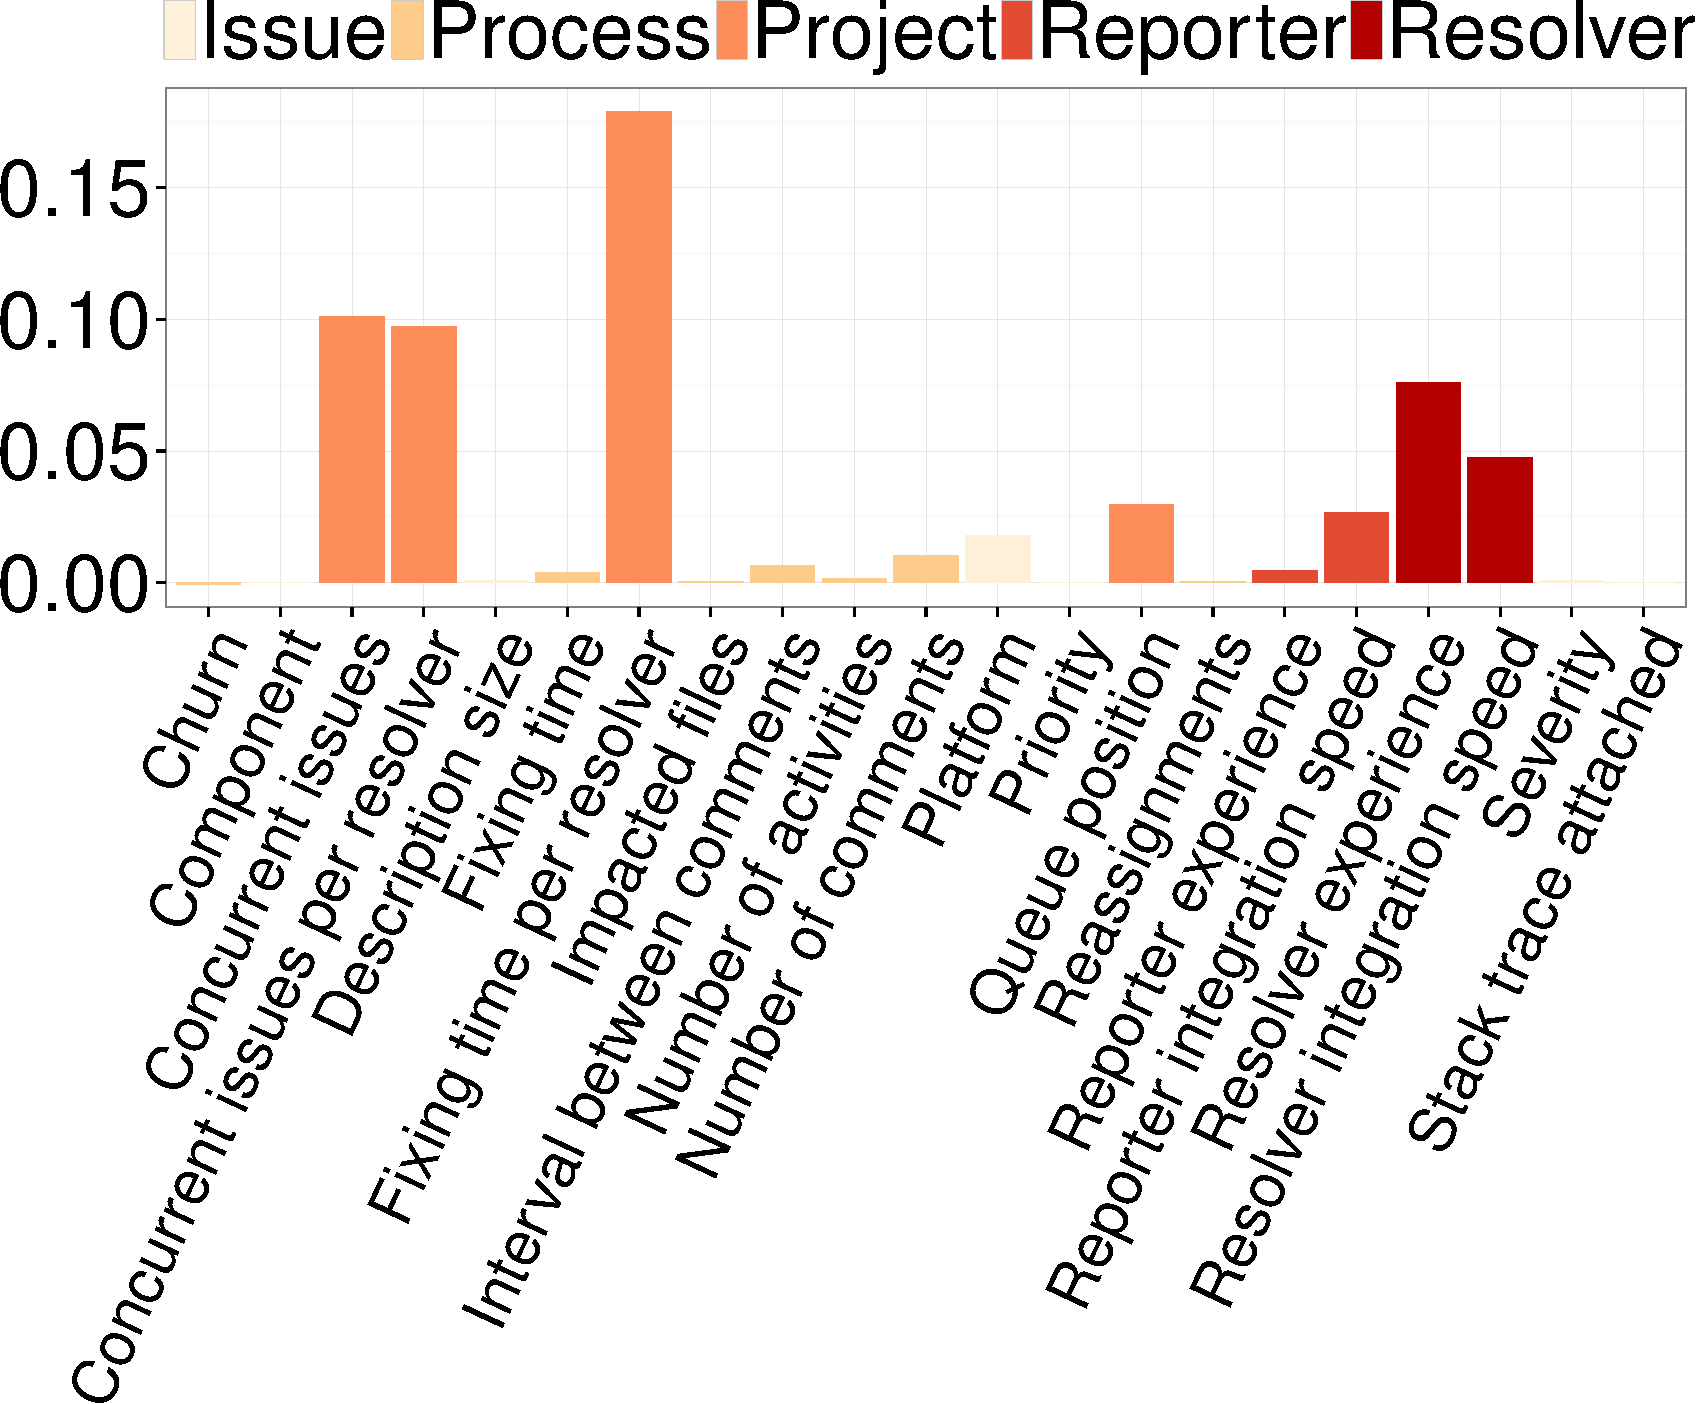
\includegraphics[width=0.55\textwidth,keepaspectratio]  
		{chapters/chapter4/figures/firefox_loocv_varimp.pdf}
		\label{ch4:fig:impFirefox}
	}

	\subfloat[ArgoUML]{
		\includegraphics[width=0.55\textwidth,keepaspectratio] 
		{chapters/chapter4/figures/argouml_loocv_varimp.pdf}
	\label{ch4:fig:impArgo}}
	\caption{\textbf{Variable importance scores.} We show the 
		importance scores that are computed for the LOOCV of our models.}
	\label{ch4:fig:variableImportance}
\end{figure}

Our results suggest that the time that is invested by the resolvers on fixing
issues have a strong association with delivery delay. This could be due to
resolvers fixing issues more carefully---which would lead to a smoother
integration of such issues---or issues that were less complex in overall (\eg a
shorter time was invested), which might simplify the integration process. A deeper
analysis of this attribute would be necessary to better understand the exact
reasons behind this relationship (\eg consulting the development team through
surveys and interviews). 

We also observe that integration workload attributes (\ie \textit{backlog of
issues} and \textit{backlog of issues per resolver}) are the second most
influential attributes in the three studied projects. This finding suggests that
the integration backlog introduces overhead that may lead to longer integration
time.

\begin{figure}[!t]
	\centering
	\includegraphics[width=0.60\textwidth,keepaspectratio]
	{chapters/chapter4/figures/firefox/RQ3_component_hm.pdf}
	\caption{\textbf{The spread of issues among the Firefox components.} The
		darker the colors, the smaller the proportion of issues that
	impact that component.}
	\label{ch4:fig:componentHeatmap}
\end{figure}

Furthermore, we study the distribution of addressed issues across components in the
Firefox project.
\hyperref[ch4:fig:componentHeatmap]{Figure}~\ref{ch4:fig:componentHeatmap} shows the top
seven components of the Firefox project, each having more than 400 addressed issues.
We analyze the proportion of addressed issues where integration was prevented in the
top seven components.
\hyperref[ch4:fig:componentHeatmap]{Figure}~\ref{ch4:fig:componentHeatmap} shows that,
for buckets \textit{next} and \textit{after-1}, the majority of issues are
related to the \textit{General component}, whereas for \textit{after-2} and
\textit{after-3-or-more} the majority are related to the \textit{Javascript
engine} component. Addressed issues related to the \textit{General} component
may be easy to integrate, whereas issues related to the \textit{Javascript
Engine} may require more careful analysis before integration.  \\


\noindent\textit{\textbf{Severity and priority have little influence on
delivery delay in terms of releases.}} Users and contributors of software
projects can denote the importance of an issue using the \textit{priority} and
\textit{severity} fields. Previous studies have shown that priority and
severity have little influence on bug fixing time
\cite{tian2015unreliability,Herraiz2008,Mockus:2002}. For example, while an
issue might be severe or of high priority, it might be complex and would take a
long time to fix.  

However, in the integration context, we expect that priority and severity would
be more influential, since the issues have already been addressed. Even though
priority and severity are often left at their default values (see
\hyperref[ch4:sec:subjects]{Section}~\ref{ch4:sec:subjects}), one would expect that the
integrators would fast-track the integration of issues for which they
care about increasing the levels of severity or priority. For instance,
according to the Eclipse project guidelines for filing issue reports, a priority
level of P1 is used for serious issues and specifies that the existence of a P1
issue should prevent a release from
shipping.\smartfoot{\url{http://wiki.eclipse.org/Development_Resources/HOWTO/Bugzilla_Use}}
Hence, it is surprising that priority and severity play such a small role in
determining the release in which an addressed issue will appear. Indeed,
\hyperref[ch4:fig:variableImportance]{Figure}~\ref{ch4:fig:variableImportance} shows
that the priority and severity metrics obtain low importance scores.

\begin{figure}
	\centering
	%\captionsetup{justification=centering}
	\subfloat[ArgoUML Priority]{
		\includegraphics[width=0.30\textwidth,keepaspectratio] 
		{chapters/chapter4/figures/argouml/RQ3_priority_hm.pdf}
	\label{ch4:fig:heatMap_argo}}
	\subfloat[Eclipse Priority]{
		\includegraphics[width=0.30\textwidth,keepaspectratio] 
		{chapters/chapter4/figures/eclipse/RQ3_priority_hm.pdf}
	\label{ch4:fig:heatMap_eclipsep}}
	\subfloat[Firefox Priority]{
		\includegraphics[width=0.30\textwidth,keepaspectratio]  
		{chapters/chapter4/figures/firefox/RQ3_priority_hm.pdf}
		\label{ch4:fig:heatMap_firefoxp}
	}

	\subfloat[Eclipse Severity]{
		\includegraphics[width=0.35\textwidth,keepaspectratio] 
		{chapters/chapter4/figures/eclipse/RQ3_severity_hm.pdf}
	\label{ch4:fig:heatMap_eclipses}}
	\subfloat[Firefox Severity]{
		\includegraphics[width=0.35\textwidth,keepaspectratio]  
		{chapters/chapter4/figures/firefox/RQ3_severity_hm.pdf}
		\label{ch4:fig:heatMap_firefoxs}
	}
	\caption{\textbf{The percentage of priority and severity levels in each
		studied bucket of delivery delay.} We expect to see light
		colour in the upper left corner of these graphs, indicating that
		high priority/severity issues are integrated rapidly.
	Surprisingly, we are not seeing such a pattern in our datasets.}
	\label{ch4:fig:heatMaps}
\end{figure}

\hyperref[ch4:fig:heatMaps]{Figure}~\ref{ch4:fig:heatMaps} shows the percentage of
issues with a given priority (\textit{y-axis}) in a given integration bucket
(\textit{x-axis}). The integration of 36\% to 97\% of priority P1 addressed issues
had their integration prevented in at least one release, whereas the integration
of 32\% to 96\% of priority P2 addressed issues were prevented from integration in
at least one release. 

In the ArgoUML project, while the majority of priority P1 issues (64\%) were
integrated in the \textit{next} release, 36\% of them had their integration
prevented in at least one release. For the Firefox project, 97\% of the P1
issues and 96\% of the \textit{blocker} issues were prevented from integration
in at least one release. Finally, for the Eclipse project, 57\% of P1 issues and
49\% of blocker issues had their integration prevented in at least one release.
Hence, our data shows that, in the context of issue integration, the
\textit{priority} and \textit{severity} values that are recorded in the ITSs
have little influence on delivery delay. Instead, addressed issues might be
prioritized by the level of risk that are associated to
them.\smartfoot{Two issues from our sample were
	promoted to stabler release channels due to low associated risk \url{https://bugzilla.mozilla.org/show_bug.cgi?id=724145} and
\url{https://bugzilla.mozilla.org/show_bug.cgi?id=732962}, while another issue was prevented from integration due to code break
\url{https://bugzilla.mozilla.org/show_bug.cgi?id=723793}.} This might explain
why the time that is invested on fixing issues during a release cycle reduces
delivery delay---a risk of an addressed issue breaking the code would be
smaller when more time is invested at fixing activities. 

\conclusionbox{The total time that is invested in fixing issues of a release
	cycle and integration workload attributes are the most influential
	attributes in our models. We also find that priority and severity have
	little influence in estimating delivery delay.}

\subsubsection*{\textbf{\textit{RQ4: Results for delivery delay in terms of days}}}

\begin{table}[t]
	\scriptsize
	\centering
	\caption{\textbf{Explanatory power of attributes.} We present the
		$\chi^2$ proportion and the degrees of freedom that are spent
		for each attribute. The $\chi^2$ of the two most influential
		attributes of each model are in bold.
	\label{ch4:tbl:explanatory_power}}
	\begin{threeparttable}
		\begin{tabular}{llrrr}
			\cline{3-5} 
			\multicolumn{2}{c}{} & 
			Eclipse &
			Firefox &
			ArgoUML
			\tabularnewline
			\hline
			\multicolumn{2}{l}{Wald $\chi^2$} & 
			$1,180$ &
			$8,560$ &
			$2,803$
			\tabularnewline
			\hline 
			\multicolumn{2}{l}{Budgeted Degrees of Freedom} &
			$87$ & 
			$879$ &
			$102$
			\tabularnewline
			\hline
			\multicolumn{2}{l}{Degrees of Freedom Spent} &
			$24$ & 
			$33$ &
			$28$
			\tabularnewline
			\hline 
			\multirow{2}{*}{Reporter experience} & 
			D.F. & 
			$1$ & 
			$1$ &
			$1$
			\tabularnewline 
			& 
			$\chi^2$ & 
			$4^{\ast\ast\ast}$ &  
			$\approx 0$ &
			$1^{\ast\ast}$
			\tabularnewline
			\hline 
			\multirow{2}{*}{Resolver experience} & 
			D.F. & 
			$1$ & 
			$1$ &
			$1$
			\tabularnewline 
			& 
			$\chi^2$ & 
			$12^{\ast\ast\ast}$ & 
			$\approx 0^{\ast}$ &  
			$\approx 0$ 
			\tabularnewline
			\hline 
			\multirow{2}{*}{Reporter integration speed} & 
			D.F. & 
			$3$ & 
			$1$ &
			$2$
			\tabularnewline &
			$\chi^2$ & 
			$16^{\ast\ast\ast}$ &
			$\approx 0$ &
			$1^{\ast}$
			\tabularnewline  
			\hline 
			\multirow{2}{*}{Resolver integration speed} & 
			D.F. & 
			$2$ & 
			$1$ &
			$4$
			\tabularnewline & 
			$\chi^2$ & 
			$\mathbf{22}^{\ast\ast\ast}$ &
			$\approx 0$ &  
			$\mathbf{9}^{\ast\ast\ast}$
			\tabularnewline
			\hline 
			\multirow{2}{*}{Fixing time} & 
			D.F. & 
			$2$ & 
			\multirow{2}{*}{$\oplus$} &
			$1$
			\tabularnewline & 
			$\chi^2$ & 
			$1^{\ast}$ &
			&  
			$1^{\ast\ast}$ 
			\tabularnewline
			\hline 
			\multirow{2}{*}{Severity} & 
			D.F. & 
			$6$ &
			$6$ &
			\multirow{2}{*}{$\ominus$} 
			\tabularnewline & 
			$\chi^2$ &
			$\approx 0$ &
			$8^{\ast\ast\ast}$ &
			%\ominus
			\tabularnewline \hline 
			\multirow{2}{*}{Priority} &
			D.F. & 
			\multirow{2}{*}{$\oslash$} & 
			$5$ &
			$5$
			\tabularnewline & 
			$\chi^2$ & 
			&%\oslash
			$5^{\ast\ast\ast}$ &  
			$1^{\ast}$  
			\tabularnewline \hline 
			\multirow{2}{*}{Description size} & 
			D.F. & 
			$1$ & 
			$1$ &
			$1$
			\tabularnewline & 
			$\chi^2$ & 
			$\approx 0$ &  
			$\approx 0$ &
			$\approx 0$
			\tabularnewline \hline 
			\multirow{2}{*}{Impacted files} & 
			D.F. & 
			$1$ &
			$1$ &
			$1$
			\tabularnewline & 
			$\chi^2$ & 
			$\approx 0$ &
			$\approx 0^{\ast\ast}$ &
			$\approx $
			\tabularnewline \hline 
			\multirow{2}{*}{Number of comments} & 
			D.F. & 
			$1$ &
			$1$ &  
			$1$
			\tabularnewline & 
			$\chi^2$ & 
			$2^{\ast\ast}$ &  
			$1^{\ast\ast\ast}$  &
			$\approx 0$
			\tabularnewline \hline 
			\multirow{2}{*}{Reassignments} & 
			D.F. & 
			$1$ & 
			$1$ &
			$1$
			\tabularnewline & 
			$\chi^2$ & 
			$\approx 0$ &  
			$\approx 0$ &
			$1^{\ast}$
			\tabularnewline \hline 
			\multirow{2}{*}{Number of activities} & 
			D.F. & 
			$1$ &
			$1$ &
			$1$
			\tabularnewline & 
			$\chi^2$ & 
			$\approx 0$ &  
			$\approx 0$ &
			$\approx 0$
			\tabularnewline \hline 
			\multirow{2}{*}{Interval between comments} & 
			D.F. & 
			$1$ &
			$1$ &
			\multirow{2}{*}{$\oslash$}
			\tabularnewline & 
			$\chi^2$ & 
			$1^{\ast}$ &  
			$\approx 0$ &
			%\oslash correlation
			\tabularnewline \hline 
			\multirow{2}{*}{Churn} & 
			D.F. & 
			$1$ &
			$1$ &
			$1$
			\tabularnewline & 
			$\chi^2$ & 
			$\approx 0$ &  
			$\approx 0$ &
			$1^{\ast\ast}$
			\tabularnewline \hline 
			\multirow{2}{*}{Number of concurrent issues} & 
			D.F. & 
			\multirow{2}{*}{$\oslash$} &
			$2$ &
			\multirow{2}{*}{$\oslash$}
			\tabularnewline &
			$\chi^2$ &
			& %\oslash
			$\mathbf{8}^{\ast\ast\ast}$ &
			%\oslash
			\tabularnewline \hline 
			\multirow{2}{*}{Number of concurrent issues per resolver} & 
			D.F. & 
			$1$ & 
			$2$ &
			$2$
			\tabularnewline &
			$\chi^2$ &
			$7^{\ast\ast\ast}$ &  
			$2^{\ast\ast\ast}$ &
			$\mathbf{9}^{\ast\ast\ast}$
			\tabularnewline \hline 
			\multirow{2}{*}{Queue position} & 
			D.F. & 
			$1$ &             
			$4$ &
			$2$
			\tabularnewline & 
			$\chi^2$ & 
			$\mathbf{23}^{\ast\ast\ast}$ & 
			$\mathbf{83}^{\ast\ast\ast}$ &
			$\mathbf{67}^{\ast\ast\ast}$
			\tabularnewline \hline 
			\multirow{1}{*}{Fixing time per resolver} & 
			D.F. & 
			$1$ & 
			$2$ &
			$4$
			\tabularnewline &
			$\chi^2$ & 
			$7^{\ast\ast\ast}$ & 
			$\approx 0^{\ast\ast}$ &
			$8^{\ast\ast\ast}$
			\tabularnewline \hline 
		\end{tabular}
		\begin{tablenotes}
		\item[$\oslash$] Discarded during correlation analysis 
		\item[$\oplus$] Discarded during redundancy analysis 
		\item[$\ominus$] The variable does not apply to the dataset
		\item[$\ast$] $p < 0.05$
		\item[$\ast\ast$] $p < 0.01$
		\item[$\ast\ast\ast$] $p < 0.001$ 
		\end{tablenotes}
	\end{threeparttable}
\end{table}

\noindent\textbf{\textit{Project family attributes, such as the backlog of
issues and queue position provide most of the explanatory power of our models.}}
\hyperref[ch4:tbl:explanatory_power]{Table}~\ref{ch4:tbl:explanatory_power} shows the
explanatory power of each of the attributes of our models. The two most
influential attributes for each model are shown in bold. \textit{Queue
position}, \ie the time at which an issue is addressed is the most influential
attribute in all of the models that are fitted to our studied projects.
Interestingly, we observe that \textit{resolver integration speed}---the median
delivery delay of the previously resolved issues of a particular
resolver---plays an influential role in our models that are fit for the Eclipse
and ArgoUML projects. Moreover, we also observe that integration workload
attributes (\ie \textit{backlog of issues}, and \textit{backlog of issues per
resolver}) are very influential in our models that are fit for the Firefox and
ArgoUML projects.\\

\begin{figure}
	\centering
	\subfloat[Eclipse]{
		\includegraphics[width=0.40\textwidth,keepaspectratio]
		{chapters/chapter4/figures/components_eclipse.pdf}
	}

	\subfloat[Firefox]{
		\includegraphics[width=0.40\textwidth,keepaspectratio]
		{chapters/chapter4/figures/components_firefox.pdf}
	}

	\subfloat[ArgoUML]{
		\includegraphics[width=0.40\textwidth,keepaspectratio]
		{chapters/chapter4/figures/components_argouml.pdf}
	}
	\caption{\textbf{Delivery delay per component.} The Figure shows the
		distributions of delivery delay in terms of days for each
		component of the studied projects.
	}
	\label{ch4:fig:component_analysis}
\end{figure}

\noindent\textbf{\textit{The component to which an issue is addressed has little
impact in the delivery delay in terms of days.}} To demonstrate this, we group
each addressed issue according to the components that such an issue modifies. We use
components that have at least 100 addressed issues as a threshold for our analysis.
We then compare the distribution of delivery delay in terms of days in these
components.
\hyperref[ch4:fig:component_analysis]{Figure}~\ref{ch4:fig:component_analysis} shows the
distributions of delivery delay in terms of days per component. We do not
observe a considerable difference between distributions of delivery delay in
the ArgoUML or Firefox projects. The distribution of the ``Other'' component in
the ArgoUML project is more skewed, which is suggestive of its generic
role---such a component may encompass a more broad spectrum of addressed issues. On
the other hand, 99\% of the addressed issues in the Eclipse (JDT) project belong to
the ``Core'' component (thus its skewness). Finally, the ``Debug'' and ``Text''
Eclipse components contain only one addressed issue each.   

\conclusionbox{The workload in terms of backlog of issues awaiting integration
	and the integration speed of prior addressed issues of a given resolver play
	a important role to model delivery delay in terms of days. Moreover,
	the initial \textit{queue position} is the most important attribute in
	all models that we fit to study delivery delay in terms of days.}




%\section{Results for Study 2} \label{ch4:study2} 

In \hyperref[ch4:study1]{Section}~\ref{ch4:study1}, we analyze integration
time with respect to the number of releases and number of days that an addressed
issue requires before integration. Additionally, we study projects with
different release cycles. For instance, in the Firefox project, we observed that
addressed issues have their integration prevented in two consecutive releases
(89\% of the addressed issues). However, a long delivery delay of one project
may be shorter than a typical integration time of another project. Hence, we set
out to complement our previous analyses by studying addressed issues that suffer
a long delivery delay when compared to other addressed issues of that particular
project.  This section addresses \hyperref[ch4:rq5]{RQ5} and
\hyperref[ch4:rq6]{RQ6}. We present the results for each RQ below.

\subsection*{\textbf{\textit{RQ5: How well can we identify the addressed issues
that will suffer from a long delivery delay?}}}

\noindent\textit{\textbf{Our models obtain 
F-measures from 0.79 to 0.96.}}
\hyperref[ch4:tbl:RFclassificationResult_ab]{Table}~\ref{ch4:tbl:RFclassificationResult_ab}
shows the performance of our exploratory models. Our models that we train for the Eclipse
project obtain the
highest F-measure (0.96). On the other hand, our models trained for the Firefox
and ArgoUML projects
obtain F-measures of 0.79 and 0.88, respectively. Moreover, our models obtain
AUC values of 0.82 to 0.96. Such results suggest that our models vastly
outperform na\"{i}ve models, such as random guessing (AUC value of 0.50).  \\

\begin{table}
	\footnotesize
	\centering
	\caption{\textbf{Performance of the random forest models.} The table
		shows the values of Precision, Recall, F-measure, and AUC values that
	are computed for the LOOCV of our models.}
	\label{ch4:tbl:RFclassificationResult_ab}
	\begin{tabular}{lccc}
		\cline{2-4} 
		& \textbf{Eclipse} & \textbf{Firefox} & \textbf{ArgoUML}\tabularnewline
		\hline 
		\textbf{Precision} & 0.97 & 0.99 & 0.98\tabularnewline
		\hline 
		\textbf{Recall} & 0.96 & 0.66 & 0.80\tabularnewline
		\hline 
		\textbf{F-measure} & 0.96 & 0.79 & 0.88\tabularnewline
		\hline 
		\textbf{AUC} & 0.96 & 0.82 & 0.89\tabularnewline
		\hline 
	\end{tabular}
\end{table}

\noindent\textit{\textbf{Our models obtain better F-measure values than
Zero-R.}} For the Eclipse, Firefox, and ArgoUML projects, Zero-R obtain median F-measures
of 0.22, 0.22, and 0.36, respectively. Meanwhile, our explanatory models obtain
F-measures of 0.96, 0.79, and 0.88, respectively. Again, such results suggest
that our models vastly outperform na\"{i}ve classification techniques.  \\

\conclusionbox{
We are able to accurately identify whether an addressed issue is likely to have
a long delivery delay in a given project. Our models outperform na\"{i}ve
techniques, such as Zero-R and random guessing, obtaining AUC values from 0.82
to 0.96 (median).
}


\subsection*{\textit{\textbf{RQ6: What are the most influential attributes for identifying the
issues that will suffer from a long delivery delay?}}}

\begin{figure}
	\centering
	\subfloat[Eclipse]{
		\includegraphics[width=0.50\textwidth,keepaspectratio] 
		{chapters/chapter4/figures/eclipse_loocv_varimp_long.pdf}
	\label{ch4:fig:impEclipse_ab}}

	\subfloat[Firefox]{
		\includegraphics[width=0.50\textwidth,keepaspectratio]  
		{chapters/chapter4/figures/firefox_loocv_varimp_long.pdf}
		\label{ch4:fig:impFirefox_ab}
	}

	\subfloat[ArgoUML]{
		\includegraphics[width=0.50\textwidth,keepaspectratio] 
		{chapters/chapter4/figures/argouml_loocv_varimp_long.pdf}
	\label{ch4:fig:impArgo}}
	\caption{\textbf{Variable importance scores.} We show the 
	importance scores that are computed for the LOOCV of our models.}
	\label{ch4:fig:variableImportance_ab}
\end{figure}


\noindent\textit{\textbf{Long delivery delay is most consistently associated with
attributes of the project family.}}
\hyperref[ch4:fig:variableImportance_ab]{Figure}~\ref{ch4:fig:variableImportance_ab}
shows the importance scores that are computed for the LOOCV that we use to
evaluate our random forest models. We observe that the attributes that are
related to the \textit{\textbf{project}} family are the most influential
attributes in the projects. The \textit{backlog of issues} is the most
influential attribute in our Eclipse models, while \textit{queue position} and
\textit{fixing time per resolver} are the most influential attributes in our
Firefox and ArgoUML models, respectively. In addition, we observe that
attributes that are related to workload, such as the \textit{backlog of issues}
and the \textit{backlog of issues per resolver} are at least the third most
influential attributes in all of our models. Such results suggest that a
\textit{long delivery delay} is associated with project-related attributes and
that the amount of addressed issues that are to be integrated also plays a major
role to identify a \textit{long delivery delay}. \\

\conclusionbox{Our explanatory models suggest that long delivery delay is more
	closely associated with project characteristics, such as
	the \textit{backlog of issues}, \textit{queue position}, and
	\textit{fixing time per resolver}. Moreover, the backlog of issues plays an
	influential role in identifying a long delivery delay in all of the studied
projects.}

\section{Discussion}\label{ch4:discussion}

\noindent\textbf{\textit{The most important attributes vary as we study
different kinds of delivery delay.}} While we observe that \textit{fixing time
per resolver} is the most influential attribute to model delivery delay in
terms of releases, the time at which an issue is addressed (\textit{queue position})
is the most influential attribute to model delivery delay in days.  This
difference may be explained by what these kinds of delivery delay highlight.
The delivery delay in terms of releases highlights the releases from which the
integration of addressed issues is prevented. In this context, the \textit{fixing
time per resolver} attribute becomes influential, since it is a measure of the
amount of time that was invested by the team to fix issues, which may lead to
smoother integration of an issue in the upcoming releases. This smoother
integration might be either because issues were addressed more carefully or because
complex/risky issues had the necessary time to become stable enough to avoid
breakage. 

On the other hand, delivery delay in terms of days highlights the total time
that is required to ship an addressed issue regardless the number of releases that
are missed. In this case, the time at which an issue is addressed in the release
cycle becomes more influential (\ie \textit{queue position}). For example, a
addressed issue might be shipped faster because it was addressed during a {\em beta
stage} (see \hyperref{ch4:rq2}{RQ2}), \ie when the collaborators have to deal with a
narrower \textit{backlog of issues} so that fixes can be performed more
carefully. The increased focus due to a narrower \textit{backlog of issues} may
lead the addressed issue to become easier to integrate in the next release cycle.

Moreover, in the Eclipse project, we observe that the speed at which the prior
addressed issues of a particular resolver are integrated influences the integration
time of new addressed issues (\textit{resolver integration speed}). This result
might be an indicator that resolvers/integrators who are experienced
in fixing and integrating fixes for the project may reduce delivery delay.

As for long delivery delay, we observe a similar behaviour in our models that
are fit to the ArgoUML and Eclipse projects. The \textit{fixing time per
resolver} attribute and attributes that are related to the \textit{backlog of
issues} are the most important to identify addressed issues that have a long
delivery delay. On the other hand, the \textit{queue position} is the most
important attribute to model long delivery delay in the Firefox project. One of
the major differences between the former projects (ArgoUML and Eclipse) and the
later one (Firefox) is the release cycle strategy that is adopted---ArgoUML and
Eclipse use a more traditional release cycle compared to the rapid release
cycles that are used in the Firefox project. Nevertheless, more empirical
analyses are necessary to investigate if there is a relationship between release
cycle strategies and prolonged delivery delay.\\

\noindent\textbf{\textit{The backlog of addressed issues awaiting integration
may introduce an overhead that needs to be managed by software teams.}} We
observe that integration workload attributes (\eg \textit{backlog of issues} and
\textit{backlog of issues per resolver}) are influential in all studied kinds of
delivery delay. This finding suggests that the overhead that is introduced by
the backlog of addressed issues that are awaiting integration may increase the
integration time as a whole. 




\section{Discussion}\label{ch4:discussion}

\noindent\textbf{\textit{The most important attributes vary as we study
different types of delivery delay.}} While we observe that \textit{fixing time
per resolver} is the most influential attribute to model delivery delay in
terms of releases, the time at which an issue is addressed (\textit{queue position})
is the most influential attribute to model delivery delay in days.  This
difference may be explained by what these types of delivery delay highlight.
The delivery delay in terms of releases highlights the releases from which the
delivery of addressed issues is prevented. In this context, the \textit{fixing
time per resolver} attribute becomes influential, since it is a measure of the
amount of time that was invested by the team to fix issues, which may lead to
smoother delivery of an issue in the upcoming releases. This smoother
delivery might be either because issues were addressed more carefully or because
complex/risky issues had the necessary time to become stable enough to avoid
breakage. 

On the other hand, delivery delay in terms of days highlights the total time
that is required to ship an addressed issue regardless the number of releases that
are missed. In this case, the time at which an issue is addressed in the release
cycle becomes more influential (\ie \textit{queue position}). For example, a
addressed issue might be shipped faster because it was addressed during a {\em beta
stage} (see \hyperref{ch4:rq2}{RQ2}), \ie when the collaborators have to deal with a
narrower \textit{backlog of issues} so that fixes can be performed more
carefully. The increased focus due to a narrower \textit{backlog of issues} may
lead the addressed issue to become easier to integrate in the next release cycle.

Moreover, in the Eclipse project, we observe that the speed at which the prior
addressed issues of a particular resolver are integrated influences the delivery
delay of new addressed issues (\textit{resolver integration speed}). This result
might be an indicator that resolvers/integrators who are experienced
in fixing and integrating fixes for the project may reduce delivery delay.

As for prolonged delivery delays, we observe a similar behaviour in our models that
are fit to the ArgoUML and Eclipse projects. The \textit{fixing time per
resolver} attribute and attributes that are related to the \textit{backlog of
issues} are the most important to identify addressed issues that have a
prolonged delivery delay. On the other hand, the \textit{queue position} is the most
important attribute to model prolonged delivery delay in the Firefox project. One of
the major differences between the former projects (ArgoUML and Eclipse) and the
later one (Firefox) is the release cycle strategy that is adopted---ArgoUML and
Eclipse use a more traditional release cycle compared to the rapid release
cycles that are used in the Firefox project. Nevertheless, more empirical
analyses are necessary to investigate if there is a relationship between release
cycle strategies and prolonged delivery delay.\\

\noindent\textbf{\textit{The backlog of addressed issues awaiting integration
may introduce an overhead that needs to be managed by software teams.}} We
observe that integration workload attributes (\eg \textit{backlog of issues} and
\textit{backlog of issues per resolver}) are influential in all studied types of
delivery delay. This finding suggests that the overhead that is introduced by
the backlog of addressed issues that are awaiting integration may increase the
delivery delay as a whole. 


\section{Exploratory Data Analysis} \label{ch4:exploratory}

\subsection{Backlog of Issues per Addressed Issue}

\begin{figure}
	\centering
	\includegraphics[width=0.85\textwidth,keepaspectratio]
	{chapters/chapter4/figures/boxplot-workloadratio-system.pdf}
	\caption{\textbf{Backlog of issues per addressed issue of the current
		release cycle.} The median number of concurrent fixes per addressed issue
	for the Eclipse, Firefox, and ArgoUML projects are 3, 2, and 1, respectively.}
	\label{ch4:fig:concurrent_issues}
\end{figure}

Since we observe that the integration workload in terms of the number of
backlog of issues is an influential attribute in all of the studied projects, we
also investigate the competition that is due to issues that are waiting for
integration per addressed issue in the release cycle.
\hyperref[ch4:fig:concurrent_issues]{Figure}~\ref{ch4:fig:concurrent_issues} shows the
distributions of the number of competing issues for an addressed issue of a
given release cycle. For each addressed issue, a median of three, two, and one
other issues are competing for integration in the Eclipse, Firefox, and ArgoUML
projects, respectively. It is interesting to note that the distribution of the
Firefox project is equivalent to the Eclipse project one, even though the
Firefox releases are more frequent. This might suggest an intense period of
activity in the Firefox release cycles (high rates of integration and fixing activity).

\subsection{Practical Suggestions}

In our study, we observe that attributes such as: \textit{fixing time per
resolver}, \textit{backlog of issues}, \textit{resolver integration speed}, and
\textit{queue position} have a considerable impact on the studied types of
delivery delay. As such, we suggest that our investigated attributes could be
used as a starting point in project management tools to track the delivery
delay of addressed issues. For example, a tool that could automatically track the
\textit{backlog of issues} by using the ITS, could raise warnings when the
backlog for integration crosses a project-specific threshold. Such a warning
could lead to early integration sessions before the official release deadline,
and prevent log jams in the integration queue. 

Our work suggests that the integration and delivery stages are also a bottleneck
that has to be managed in a software project. Tracking data and developing tools
to reduce delivery delay should also be the target of the practice and research.


\section{Threats to Validity} \label{ch4:threats}

\subsection{Construct Validity}
A number of tools were developed in order to extract and analyze the delivery
delay data in the studied projects. Defects in these tools could have an influence on
our results. However, we carefully tested our tools using manually-curated
subsamples of the studied projects, which produced correct results.

\subsection{Internal Validity}
The internal threats to validity are concerned with the ability to draw
conclusions from the relation between the explanatory and response variables.

The main threat in this regard is the representativeness of the data. Although
the Firefox and Eclipse projects report the list of addressed issues in their
release notes, we do not know how complete this list truly is. In addition,
issues may be incorrectly listed in a release note. For example, an issue that
should have been listed in the release notes for version 2.0 but only appears in
the release note for version 3.0. Such human errors may introduce noise in our
datasets. To explore how correct the release notes are, we draw a random sample
of 120 Firefox addressed issues, each one listed in the release notes of
versions 17 to 27. We verify the corresponding \textit{tag} that such issues
were integrated into in the BETA channel, \ie the most stable channel of the
Firefox project that lead to the RELEASE
channel.\smartfoot{\url{https://hg.mozilla.org/releases/mozilla-beta/tags}}
Indeed, 94\% ($\frac{113}{120}$) addressed issues were integrated into the
corresponding tag that lead to the release for which the release notes have
listed such issues. This sample can be found on the supplemental material web
page.\smartfoot{\url{http://sailhome.cs.queensu.ca/replication/integration_delay/}}

Another threat is the method that we use to map the addressed issues to releases in
the ArgoUML project. This mapping is based on the \textit{target\_milestone}
which may be more susceptible to human error. Nonetheless, our results obtained
for the Firefox and Eclipse projects are based on addressed issues that have been
denoted in the release notes---and that we are more confident about their
delivery delay.

In addition, the way that we segment the response variable of our explanatory
models is also subject to bias. For the delivery delay in terms of releases
(\hyperref[def:1]{Definition}~\ref{def:1}), we segment the response variable
into \textit{next}, \textit{after-1}, \textit{after-2}, and
\textit{after-3-or-more}. Although we found it to be a reasonable
classification, a different classification may yield different results. Also, we
use at least one MAD above the median as a threshold to split the response
variable of the prolonged delivery delay
(\hyperref[def:3]{Definition}~\ref{def:3}) into two categories. A different
threshold to split the response variable may yield different results.

Moreover, the attributes that we considered in our explanatory models are not
exhaustive. We choose a starting set of attribute families that can be easily
computed through publicly available data sources such as ITSs and VCSs. The
addition of other attributes would likely improve model performance. For
instance, one could study testing or code review effort that was
invested on an addressed issue. Nonetheless, our random forest models performed well
compared to random guessing and Zero-R models with the current set of attributes
and response variable segmentation. With respect to our linear regression
models, we base our observations using models that obtain 39\% to 65\% of
variability explained. Although higher $R^2$ values are usually targeted in
research, we provide a sound starting point of regression models for studying
delivery delay phenomena---especially in a field that involves human
intervention, such as software engineering.

Finally, the main limitation of our statistical models (\ie random forests and
linear regressions) is that we cannot claim a causal relationship between our
explanatory variables (\ie the studied attributes) and delivery delay.
Instead, our conclusions are based on associations that are drawn from the
average behavior of our studied projects' data.

\subsection{External Validity}
External threats are concerned with our ability to generalize our results. In
our work, we investigated only three open source projects. Although the projects
that we considered in our study are of different sizes and domains, and
prescribing to different release policies, our findings may not generalize to
other projects. Replication of this work in a large set of projects is required
in order to reach more general conclusions.


%\section{Related Work} \label{ch4:relatedwork}

In this chapter, we present our studies regarding the general delivery delay of
addressed issues. Hence, we outline related work about possible delays that can
be related to software issues.

Jiang \etal \cite{Jiang2013} studied attributes that could determine the
acceptance and integration of a patch into the Linux kernel. A patch is a record
of changes that is applied to a software system to address an issue. To identify
such attributes, the authors built decision tree models and conducted top node
analysis. Among the studied attributes, developer experience, patch maturity,
and prior subsystem are found to play a major role in patch acceptance and
integration time. Choetkiertikul~\etal~\cite{riskyissues2015a,riskyissues2015b}
study the risk of issues introducing delays that can postpone the shipment of
new releases of a software project. The authors use local attributes (\ie
attributes that can be collected in the issue report itself) and network
attributes (\ie attributes that are extracted from the relationship between
issues) to perform their analyses.

Similar to Jiang \etal\cite{Jiang2013}, we also investigate the integration of
addressed issues.  However, we focus on the delivery delay of issues that are
already addressed rather than the probability to accept a particular patch.
Differently from Choetkiertikul~\etal~\cite{riskyissues2015a,riskyissues2015b},
we study the attributes that may induce addressed issues to be prevented from
delivery rather than the risk of postponing an upcoming release.


\section{Conclusions}\label{ch4:conclusion} Once an issue is
addressed, what users and code contributors care most about is when the software
is going to reflect such an addressed issue, \ie when such an addressed issue is
delivered. However, we observed that the delivery of several addressed issues
was prevented for a considerable amount of time. In this context, it is not clear why certain
addressed issues take longer to be integrated than others. We performed
an empirical study of 20,995 issues from the ArgoUML, Eclipse and Firefox
projects. In our study, we:
\\
	\begin{itemize}
		\item despite being addressed well before an upcoming release, 34\% to
			60\% of the addressed issues are not integrated in more than one
			release in the ArgoUML and Eclipse projects. Furthermore, 98\%
			of the Firefox project issues had their delivery delayed by
			at least one release. \\

		\item train random forest models to model the delivery
			delay of an addressed issue. Our models obtain a
			median AUC values between 0.62 to 0.96. Our models
			outperform baseline random and Zero-R models. \\

		\item compute variable importance 
			to understand which attributes are the most important in
			our random forest models to study delivery delay.
			Heuristics that estimate the effort that teams invest in
			fixing issues are the most influential in
			our models to study delivery delay in terms of number of
			releases. \\
			
		\item find that, surprisingly, \textit{priority} and
			\textit{severity} have little impact on our exploratory
			models for delivery delay.
			Indeed, 36\% to 97\% of priority P1 addressed issues
			were delayed by at least one release. \\ 

		\item find that a shorter delivery delay is associated with
			fixes that are performed during more controlled stages
			of a given release cycle.\\

		\item observe that the time at which issues are addressed and the
			resolvers of the issues have great impact on estimating
			the delivery delay of an addressed issue.  Our explanatory
			models obtain $R^2$ values between 0.39 to 0.65. \\

		\item verify that our models that identify addressed issues that
			have a prolonged delivery delay outperform random
			guessing and Zero-R models, obtaining AUC values of 0.82~to~0.96.\\

		\item find that the time at which an issue is addressed (queue
			position), the integration workload (in terms of the
			backlog of addressed issues), and the
			heuristics that estimate the effort that teams invest in
			fixing issues (fixing time per resolver), are the
			most influential attributes for issues that have 
			a prolonged delivery delay. \\

	\end{itemize}

Our work provides insights as to why some addressed issues are integrated prior
to others. Our results suggest that characteristics of the release cycle are the
ones that have the largest impact on delivery delay. Therefore, our findings
highlight the importance of future research and tooling that can support
integrators of software projects. It is important to improve the integration and
delivery stages of a release cycle, since the availability of an addressed issue
in a release is what users and contributors care most about. 




\chapter[Do Rapid Releases Reduce Delivery Delay?]{Do Rapid Releases Reduce
Delivery Delay?} \label{ch:study34}

\keybox{An earlier version of
\hyperref[st:study3]{Study}~\ref{st:study3} appear in the proceedings of the
International Conference on Mining Software Repositories
(MSR'16)~\cite{da2016impact}.} 
%Also,
%the current \hyperref[st:study3]{Studies}~\ref{st:study3} and~\ref{st:study4}
%compose an extended version of our prior MSR'16 work and is currently under
%review in the Journal of Empirical Software Engineering.}

\section{Introduction} \label{sec:introduction}

Within the context of constantly evolving requirements (e.g., in \textit{agile}
development), approaches like eXtreme Programming (XP) and Scrum have arisen to
foster faster software
delivery~\cite{beck2000extreme}.\smartfoot{\url{http://www.scrumguides.org/}}
Those methodologies claim to better embrace a constantly evolving requirements
context by shortening release cycles. Indeed, modern release cycles are on the
order of days or weeks rather than months or years~\cite{baskerville2004short}.
Such rapid releasing enables faster user feedback and a smoother roadmap for
user adoption.

The allure of delivering new features faster has led many large software
projects to shift from a more traditional release cycle (\eg 12-18 months to
ship a major release), to shorter release cycles (\eg weeks). For example,
Google Chrome, Mozilla Firefox, and Facebook teams have each adopted shorter release
cycles~\cite{adams2016saner}. In this chapter, we use the terms \textit{rapid releases} to describe
releases that are shipped using release cycles of weeks or days, and \textit{traditional
releases} to describe releases that are shipped using release cycles of months or years. 

Prior research has investigated the impact of adopting rapid
releases \cite{mantyla2014rapid,souza2014rapid,souzabackout,baysal2011tale,khomh2012faster}.
For example, Khomh~\etal \cite{khomh2012faster} found that bugs that are related to crash
reports tend to be fixed more quickly in the rapid Firefox releases than the traditional
ones. M\"antyl\"a~\etal~\cite{mantyla2014rapid} found that the
Firefox project's shift from a traditional to a rapid release cycle has been
accompanied by an increase in the testing workload.
 
To the best of our knowledge, little prior research has empirically studied the
impact that a shift from a traditional to a rapid release cycle has on the speed
of delivering addressed issues. Such an investigation is important to
empirically check if adopting a rapid release cycle really does lead to the
quicker delivery of addressed issues. In
\hyperref[ch:study12]{Chapter}~\ref{ch:study12}, we study the delay that
happens before the delivery of an addressed issue. We found that 98\% of the
addressed issues in the rapid releases of Firefox were prevented from delivery
in at least one release. Such delayed deliveries hint that even though rapid
releases are consistently shipped every 6 weeks, they may not be delivering
addressed issues as quickly as its proponents purport.

Hence, in this chapter, we compare traditional and rapid release cycles with
respect to delivery delay. We perform a quantitative analysis of 72,114 issue
reports from the Firefox project (34,673 for traditional releases and 37,441 for
rapid releases). These issue reports refer to bugs, enhancements, and new
features~\cite{giuliano2008}. We address the following RQs:
%
%In the second study, we set out to qualitatively
%analyze the delivery delay of addressed issues by surveying 37 participants from
%the Firefox, Eclipse, and ArgoUML projects.

\begin{itemize}

	\item \textbf{\textit{RQ1: Are addressed issues delivered more quickly
		in rapid releases?}} Interestingly, we find that although issues
		are addressed more quickly in rapid releases, they tend to
		require a longer time to be delivered to users.\\

	\item \textbf{\textit{RQ2: Why can traditional releases deliver
		addressed issues more quickly?}} We find that minor-traditional
		releases (\ie releases of smaller scope that are shipped after a
		major version of the software) are a key reason as to why
		addressed issues tend to be delivered more quickly in
		traditional releases. In addition, we find that the length of
		the release cycles are roughly the same between traditional and
		rapid releases when considering both minor and major releases,
		with medians of 40 and 42 days, respectively.\\

	\item \textbf{\textit{RQ3: Did the change in release strategy have an
		impact on the characteristics of delayed issues?}} Our models
		suggest that issues are queued up as a project backlog in
		traditional releases, while issues in rapid releases are queued
		up on a per release basis (\ie a backlog per release cycle).
		Issues that are addressed early either in a project or release
		cycle backlog are less likely to be delayed.
\end{itemize}  

\noindent \textbf{Chapter Organization.} The remainder of this chapter is
organized as follows. In
\hyperref[sec:studysettings]{Section}~\ref{sec:studysettings}, we describe the
design of this study. In \hyperref[ch4:results]{Section}~\ref{ch4:results}, we
present the obtained results. In
\hyperref[sec:discussion]{Section}~\ref{sec:discussion}, we analyze potential
confounding factors that are related to our results. In
\hyperref[sec:guidelines]{Section}~\ref{sec:guidelines}, we suggest practical
guidelines based on our study. Finally, we disclose the threats to the validity
of our study in \hyperref[sec:threats]{Section}~\ref{sec:threats} and we draw
conclusions in \hyperref[sec:conclusion]{Section}~\ref{sec:conclusion}. 


\section{Methodology} \label{sec:studysettings}
%We present two studies in this chapter: a quantitative and a qualitative study
%(\hyperref[st:study3]{Studies}~\ref{st:study3} and \ref{st:study4},
%respectively).  

In \hyperref[st:study3]{Study}~\ref{st:study3}, we set out to comparatively
analyze the delivery delay in terms of days (see
\hyperref[def:2]{Definition}~\ref{def:2}) of addressed issues that were shipped
in traditional releases versus the ones that were shipped in rapid releases. In
this section, we provide information about the subject projects, data collection
process, and how we perform the analyses of our study.

\subsection{Subjects}

We choose to study the Firefox project because it offers a unique opportunity to
investigate the impact of shifting from a traditional release cycle to a rapid
release cycle using rich, publicly available ITS and \textit{Version Control
System} (VCS) data. Although other open source projects may have ITS and VCS
data available, they do not provide the opportunity to investigate the
transition between traditional releases and rapid releases. In addition,
comparing different projects that use traditional and rapid releases poses a
great challenge, since one has to distinguish to what extent the results are due
to the release strategy and not due to intricacies of the projects themselves.
Therefore, we highlight that the choice to investigate Firefox is not
accidental, but based on the specific analysis constraints that such data
satisfies, and the very unique nature of such data.

\subsection{Data Collection}\label{ch5:datacollection}

\hyperref[fig:database_construction]{Figure}~\ref{fig:database_construction}
shows an overview of our data collection approach. Each step of the process is
described below.

\begin{figure}[!]
	\centering
	\includegraphics[width=0.90\textwidth,keepaspectratio]
	{chapters/chapter5/figures/database_construction_final.pdf}
	\caption{
		Overview of the process to construct the dataset that is used in
		our \hyperref[st:study3]{Study}~\ref{st:study3}.
	}
	\label{fig:database_construction}
\end{figure}

\begin{table}[!]
	\footnotesize
	\centering
	\caption{The studied traditional and rapid Firefox releases.
	\label{tbl:releases}}
		\begin{tabular}{ccccc}
			\hline 
			\textbf{Strategy} & \textbf{Version range} &
			\textbf{Time period} & \textbf{\# of Majors} &
			\textbf{\# of Minors}\tabularnewline
			\hline 
			\hline 
			Trad. & 1.0 - 4.0 & Sep/2004 - Mar/2012 & 7 & 104\tabularnewline
			\hline 
			Rapid & 5 - 27 & Jun/2011 - Sep/2014 & 23 & 50\tabularnewline
			\hline 
		\end{tabular}%
	%	}
\end{table}

\noindent\textbf{\textit{Step 1: Collect release information.}} We collect the date and
version number of each Firefox release (minor and major releases of each release
strategy) using the Firefox release history
wiki.\smartfoot{\url{https://en.wikipedia.org/wiki/Firefox_release_history}}
\hyperref[tbl:releases]{Table}~\ref{tbl:releases} shows: {\em (i)}the range of versions of releases that we
investigate, {\em (ii)} the investigated time period of each release strategy, and
(iii) the number of major and minor studied releases in each release strategy.\\

\noindent\textbf{\textit{Step 2: Link issues to releases.}} Once we collect the release
information, we use the \textit{tags} within the VCS to link issue IDs to
releases.  First, we analyze the tags that are recorded within the VCS. Since
Firefox migrated from CVS to Mercurial during release 3.5, we collect the tags
of releases 1.0 to 3.0 from CVS, while we collect the tags of releases 3.5 to 27
from
Mercurial.\smartfoot{\url{http://cvsbook.red-bean.com/cvsbook.html}}$^,$\smartfoot{\url{https://mercurial.selenic.com/}}
By analyzing the tags, we extract the commit logs within each tag. The extracted
commit logs are linked to their respective tags. We then parse the commit logs
to collect the issue IDs that are being addressed in the commits. We discard the
following patterns of potential issue IDs that are false positives:

\begin{enumerate}
\item Potential IDs that have less than five digits, since the issue IDs of the
	investigated releases should have at least five digits (2,559 issues
	were discarded).  
\item Commit logs that follow the pattern: ``Bug $<$ID$>$ -
	reftest'' or ``Bug $<$ID$>$ - JavaScript Tests'',
	which refer to tests and not bug fixes (269 issues were
	discarded).  
\item Any potential ID that is the name of a file, \eg
	``159334.js'' (607 issues were discarded).
\end{enumerate}          

We find that all of the remaining IDs match issue IDs that exist in the Firefox
ITS.

Since the commit logs are linked to VCS tags, we are also able to link the
issue IDs found within these commit logs to the releases that correspond to
those tags. For example, since we find the fix for issue 529404 in the commit
log of tag 3.7a1, we link this issue~ID to that release. We also merge together
the data of development releases like 3.7a1 into the nearest minor or major
release. For example, release 3.7a1 would be merged with release 4.0, since it
is the next user-intended release after 3.7a1. In the case that a particular
issue is found in the commit logs of multiple releases, we consider that
particular issue to pertain to the earliest release that contains the last fix
attempt (commit log), since that release is the first one to contain the
complete fix for the issue. Finally, we collect the issue report information
of each remaining issue (\eg opening date, fix date, severity, priority, and
description) using the ITS. Moreover, since the minor-rapid releases are
\textit{off-cycle releases}, in which addressed issues may skip being integrated
into \code{mozilla-central} (\ie NIGHTLY) tags, we manually collect the addressed
issues that were integrated into those releases using the Firefox release notes
(\ie 247 addressed~issues).\smartfoot{\url{https://www.mozilla.org/en-US/firefox/releases/}}
We add the manually collected addressed issues from ESR releases within the rapid
releases data, since they also represent data from a rapid release strategy.\\

\noindent\textbf{\textit{Steps 3 and 4: Compute metrics and perform analyses.}}
We use the data from Step 2 to compute the metrics that we use in our analyses.
We select these metrics (which are described in the
\hyperref[ch5:rq3]{approach for RQ3}) because we suspect that they
share a relationship with delivery delay.

\section{Results} \label{ch4:results}

In this study, we address three research
questions about the shift from a traditional to a rapid release cycle. The
motivation of each research question is detailed below.

\subsection{RQ1: Are addressed issues delivered more quickly in rapid
releases?}\label{ch5:rq1} 

\subsubsection*{RQ1: Motivation} 

Since there is a lack of empirical evidence to indicate that rapid release
cycles deliver addressed issues more quickly than traditional release cycles, we
compare the delivery delay of addressed issues in traditional releases against
the delivery delay in rapid releases in \hyperref[ch5:rq1]{RQ1}.\\

\subsubsection*{RQ1: Approach}

\begin{figure}[t!]
	\centering
	\includegraphics[width=\columnwidth,keepaspectratio]
	{chapters/chapter5/figures/rq1/issue_lifecycle.pdf}
	\caption{A simplified life cycle of an issue.}
	\label{fig:issue_lifecycle}
\end{figure}

\hyperref[fig:issue_lifecycle]{Figure}~\ref{fig:issue_lifecycle} shows a
simplified life cycle of an issue, which includes the triaging phase ({\em t1}),
the fixing phase ({\em t2}), and the integration phase ({\em t3}). We consider
the last RESOLVED-FIXED status as the moment at which a particular issue was
addressed (the fixed state in
\hyperref[fig:issue_lifecycle]{Figure}~\ref{fig:issue_lifecycle}). The
\textit{lifetime} of an issue is composed of all three phases (from \textit{new}
to \textit{released}). For \hyperref[ch5:rq1]{RQ1}, we first observe the lifetime of the issues of
traditional and rapid releases.  Next, we look at the time span of the
\textit{triaging}, \textit{fixing}, and \textit{integration} phases within the
lifetime of an issue.

We use beanplots~\cite{kampstra2008beanplot} to compare the distributions of our
data. The vertical curves of beanplots summarize and compare the distributions
of different datasets (see
\hyperref[fig:delivery_delay]{Figure}~\ref{fig:delivery_delay}). The higher
the frequency of data within a particular value, the thicker the bean is plotted
at that particular value on the $y$ axis. We also use Mann-Whitney-Wilcoxon
(MWW) tests~\cite{wilks2011statistical} and Cliff's delta effect-size
measures~\cite{cliff1993dominance}. MWW tests are non-parametric tests of the
\textit{null hypothesis} that two distributions come from the same population
($\alpha=0.05$). On the other hand, Cliff's delta is a non-parametric
effect-size measure to verify the difference in magnitude of one distribution compared
to another distribution. The higher the value of the Cliff's delta,
the greater the difference of values between distributions. For instance, if we
obtain a significant $p$ value but a small Cliff's delta, this means that
although two distributions do not come from the same population their 
difference is not that large. A positive Cliff's delta indicates how much
larger the values of the first distribution are, while a negative Cliff's delta
indicates the inverse. Finally, we use the \textit{Median Absolute Deviation}
(MAD) \cite{howell2005median,leys2013detecting} as a measure of the variation of
our distributions. The MAD is the median of the \textit{absolute deviations}
from one distribution's median. The higher the MAD, the greater is the variation
of a distribution with respect to its median.

\subsubsection*{RQ1: Results}

\begin{figure}[t!]
	\centering
	\subfloat[Lifetime]{
		\includegraphics[width=.45\columnwidth,keepaspectratio]
		{chapters/chapter5/figures/rq1/trad-vs-rapid-entire.pdf}
		\label{fig:delivery_delay}
	}
	\subfloat[Triaging phase]{
		\centering
		\includegraphics[width=.45\columnwidth,keepaspectratio]
		{chapters/chapter5/figures/rq1/traditional_vs_rapid_triaging.pdf}
		\label{fig:triaging}
	}

	\subfloat[Fixing phase]{
		\centering
		\includegraphics[width=.45\columnwidth,keepaspectratio]
		{chapters/chapter5/figures/rq1/traditional_vs_rapid_fixtime.pdf}
		\label{fig:fixtime}
	}
	\subfloat[Integration phase]{
		\centering
		\includegraphics[width=.45\columnwidth,keepaspectratio]
		{chapters/chapter5/figures/rq1/traditional_vs_rapid.pdf}
		\label{fig:traditional_vs_rapid}
	}
	\caption{Time spans of the phases involved in the lifetime of an issue.}
	\label{fig:timespans}
\end{figure}

\noindent\finding{There is no significant difference between traditional and
rapid releases regarding issue lifetime.}{find17}
\hyperref[fig:delivery_delay]{Figure}~\ref{fig:delivery_delay} shows the
distributions of the lifetime of the issues in traditional and rapid releases.
We observe a $p<1.03e^{-14}$ but a $negligible$ difference between the
distributions ($\textit{delta}=0.03$). We also observe that traditional releases
have a greater MAD ($154$ days) than rapid releases ($29$ days), which indicates
that rapid releases are more consistent with respect to the lifetime of the
issues. Our results indicate that the difference in the issues' lifetime between
traditional and rapid releases is not as obvious as one might expect. We then
look at the triaging, fixing, and integration time spans to better understand
the differences between traditional and rapid releases.\\

\noindent\finding{Addressed issues are triaged and fixed more quickly in rapid
releases, but tend to wait for a longer time before being delivered.}{find18}
\hyperref[fig:triaging]{Figures}~\ref{fig:triaging}~,~\ref{fig:fixtime},~and~\ref{fig:traditional_vs_rapid}
show the triaging, fixing, and integration time spans, respectively. We observe
that addressed issues take a median time of 54 days to be integrated into
traditional releases, while taking 104 days (median) to be integrated into rapid
releases. We observe a $p<2.2e^{-16}$ with a $small$ effect-size
($delta=-0.25$).

Regarding fixing time span, an issue takes 6 days (median) to be fixed in rapid
releases, and 9 days (median) in traditional releases. These results are
statistically significant $p<2.2e^{-16}$, but there is only a $negligible$
difference between distributions ($delta=0.13$). 

Our results complement previous research. Khomh~\etal \cite{khomh2012faster}
found that post- and pre-release bugs that are associated with crash reports are
fixed faster in rapid Firefox releases than in traditional releases.
Furthermore, we observe a significant $p<2.2e^{-16}$ but $negligible$ difference
($\textit{delta}=0.11$) between traditional and rapid releases regarding
triaging time. The median triaging time for rapid and traditional releases are
11 and 18 days, respectively.

When we consider both pre-integration phases together (triaging $t1$ plus fixing
$t2$ in \hyperref[fig:issue_lifecycle]{Figure}~\ref{fig:issue_lifecycle}), we
observe that an issue takes $11$ days (median) to triage and address in rapid
releases, while it takes $19$ days (median) in traditional releases. We observe
a $p<2.2e^{-16}$ with a $small$ effect-size ($delta=0.15$). Our results suggest
that even though issues have shorter pre-integration phases in rapid releases,
they remain ``on the shelf'' for a longer time on average.

Finally, we again observe that rapid releases are more consistent than
traditional releases in terms of fixing and delivery rate. Rapid releases
achieve MADs of 9 and 17 days for fixing and delivery, respectively. The values
for traditional releases are 13 and 64 days for fixing and delivery,
respectively.\\ 

\conclusionbox{Although issues are triaged and fixed faster in rapid releases,
they tend to take a longer time to be integrated. However, the delivery rate
of addressed issues is more consistent in rapid releases than in traditional
ones.}

\subsection{RQ2: Why can traditional releases deliver addressed issues
more quickly?}\label{ch5:rq2} 

\subsubsection*{RQ2: Motivation} 

In \hyperref[ch5:rq1]{RQ1}, we surprisingly find that traditional releases tend
to deliver addressed issues more quickly than rapid releases. This result raises
the following question: why can a traditional release strategy, which has a
longer release cycle, deliver addressed issues more quickly than a rapid
release~strategy?\\

\subsubsection*{RQ2: Approach}

In \hyperref[ch5:rq2]{RQ2}, we group traditional and rapid releases into major
and minor releases and study their delivery delays. As in
\hyperref[ch5:rq1]{RQ1}, we also use beanplots~\cite{kampstra2008beanplot}, MWW
tests~\cite{wilks2011statistical}, and Cliff's delta effect-size
measures~\cite{cliff1993dominance} to perform our comparisons.

\subsubsection*{RQ2: Results}

\begin{figure}[t!]
	\centering
	\includegraphics[width=\textwidth,keepaspectratio]
	{chapters/chapter5/figures/rq2/major_vs_minor.pdf}
	\caption{
		Distributions of delivery delay of addressed issues grouped by minor and major
		releases.
	}
	\label{fig:major_vs_minor}
\end{figure}

\begin{sloppypar}
\noindent\finding{Minor-traditional releases tend to have
less delivery delay than major/minor-rapid releases.}{find19}
\hyperref[fig:major_vs_minor]{Figure}~\ref{fig:major_vs_minor} shows the distributions of delivery delay
grouped by (1) \textit{major-traditional vs. minor-traditional}, (2)
\textit{major-traditional vs. rapid}, (3) \textit{major-rapid vs. minor-rapid},
and (4) \textit{minor-traditional vs. minor-rapid}. In the comparison of
\textit{major-traditional vs.  minor-traditional}, we observe that
minor-traditional releases are mainly associated with shorter delivery delay.
Furthermore, in the comparison \textit{major-traditional vs. rapid}, rapid
releases deliver addressed issues more quickly than major-traditional releases
on average ($p<2.2e^{-16}$ with a $medium$ effect-size, \ie  $delta=0.40$). 
\end{sloppypar}

The Firefox rapid release cycle includes ESR releases (see
\hyperref[ch:background]{Chapter}~\ref{ch:background}) and a few minor
stabilization and security releases. These releases also deliver addressed
issues more quickly than major-rapid releases (\textit{major-rapid vs.
minor-rapid}) with a $p<2.2e^{-16}$ and a $large$ effect-size, \ie $delta=0.92$.
Furthermore, we do not observe a statistically significant difference between
distributions in the comparison of \textit{minor-traditional vs. minor-rapid}
($p=0.68$).

Minor-traditional releases have the lowest delivery delay (median of 25
days). This is likely because they are more focused on a particular set of
issues that, once addressed, should be released immediately. For example, the
release history documentation of Firefox shows that minor releases are usually
related to stability and security
issues.\smartfoot{\url{https://www.mozilla.org/en-US/firefox/releases/}}\\

\begin{figure}[t!]
	\centering
	\subfloat[Only Major]{           
		\includegraphics[width=0.45\columnwidth,keepaspectratio]
		{chapters/chapter5/figures/releases/majorreleases_length.pdf}
		\label{fig:majorreleases_length}
	}
	\subfloat[Major and Minor]{
		\includegraphics[width=0.45\columnwidth,keepaspectratio]
		{chapters/chapter5/figures/releases/releases_length.pdf}
		\label{fig:releases_length}
	}
	\caption{Release frequency (in days). The outliers in figure~(b)
		represent the major-traditional releases.}
	\label{fig:release_length_analysis}
\end{figure}

\noindent\finding{When considering both minor and major releases, the time span
between traditional and rapid releases are roughly the same.}{find20} Since we
observe that delivery delay is shorter on average in traditional releases, we
also investigate the length of the release cycles to better understand our
previous results (see \hyperref[find19]{Finding}~\ref{find19}).
\hyperref[fig:majorreleases_length]{Figure}~\ref{fig:majorreleases_length} shows
that, at first glance, one may speculate that rapid releases should deliver
addressed issues more quickly because releases are produced more frequently.
However, if we consider both major and minor releases---as shown in
\hyperref[fig:releases_length]{Figure}~\ref{fig:releases_length}---we observe
that both release strategies deliver releases at roughly the same rate on
average (median of $40$ and $42$ days for traditional and rapid releases,
respectively).\\

\conclusionbox{
Minor-traditional releases are one of the main reasons why the traditional
release strategy can deliver addressed issues more quickly than the rapid
release strategy. Furthermore, the lengths of the release cycles are roughly the
same between traditional and rapid releases when both minor and major releases
are considered.
}

\subsection{RQ3: Did the change in the release strategy have an impact on
the characteristics of delayed issues?}\label{ch5:rq3} 

\subsubsection*{RQ3: Motivation}

In \hyperref[ch5:rq1]{RQ1} and \hyperref[ch5:rq2]{RQ2}, we study the differences
between rapid and traditional releases with respect to delivery delay. We find
that although issues tend to be addressed more quickly in rapid releases, they
tend to wait longer to be delivered. We also find that the use of minor releases
is a key reason as to why traditional releases may deliver addressed issues more
quickly. In \hyperref[ch4:rq3]{RQ3}, we investigate what are the characteristics
of each release strategy that are associated with delivery delays. This
important investigation sheds light on what may generate delivery delays in each
release strategy, so that projects are aware of the characteristics of rapid
releases versus traditional releases before choosing to adopt one of these
release strategies. 

\subsubsection*{RQ3: Approach}

\begin{table}[!t]
	\footnotesize
	\caption{Metrics that are used in our explanatory models (Reporter, Resolver,
		and Issue families).
	\label{tbl:factors1}}
	\centering
		\begin{tabular}{rp{2cm}lp{9cm}}
			\hline
			\multicolumn{1}{c}{\textbf{Family}} &
			\multicolumn{1}{c}{\textbf{Metrics}} & \multicolumn{1}{c}{\textbf{Value}} &
			\multicolumn{1}{c}{\textbf{Definition (d)$\vert$Rationale (r)}}
			\\ \hline
			\multicolumn{ 1}{r}{\textbf{Reporter}} & Experience & Numeric & 
			\begin{tabular}{p{8.7cm}}
				\textbf{d:} the number of previously delivered issues that were reported by
				the reporter of a particular addressed issue.  \\ \hline 
				\textbf{r:} The greater the experience of the reporter the
				higher the quality of his/her reports and the
				solution to his/her reports might be delivered
				more quickly~\cite{shihab2010predicting}.
			\end{tabular}
			\\ \cline{2- 4}
			\multicolumn{ 1}{r}{} & Reporter integration & Numeric &
			\begin{tabular}{p{8.7cm}}
				\textbf{d:} The median in days of the previously delivered addressed issues
				that were reported by a particular reporter.
				\\ \hline 
				\textbf{r:} If a particular reporter usually reports issues that are
				delivered quickly, his/her future reported issues might be delivered
				quickly as well.
			\end{tabular}
			\\ \hline
			\multicolumn{ 1}{r}{\textbf{Resolver}} & Experience & Numeric & 
			\begin{tabular}{p{8.7cm}}
				\textbf{d:} the number of previously delivered addressed issues that were
				addressed by the resolver of a particular
				addressed issue. We consider the collaborator
				that changed the status of an issue to
				RESOLVED-FIXED as the resolver of that issue. \\ \hline 
				\textbf{r:} The greater the experience of the resolver, the
				greater the likelihood that his/her code will be
				delivered faster~\cite{shihab2010predicting}.
			\end{tabular}
			\\ \cline{2- 4}
			\multicolumn{ 1}{r}{} & Resolver integration & Numeric &
			\begin{tabular}{p{8.7cm}}
				\textbf{d:} The median in days of the previously delivered addressed issues
				that were addressed by a particular resolver.
				\\ \hline 
				\textbf{r:} If a particular resolver usually address issues that are
				delivered quickly, his/her future addressed issues might be delivered
				quickly as well.
			\end{tabular}
			\\ \hline
			\multicolumn{ 1}{r}{\textbf{Issue}} & Stack trace attached & Boolean &
			\begin{tabular}{p{8.7cm}}
				\textbf{d:} We verify if the issue report has a stack trace attached in its description. \\ \hline 
				\textbf{r:} A stack trace attached may provide useful information regarding
				the cause of the issue, which may quicken the
				delivery of the addressed issue~\cite{schroter2010stack}. 
			\end{tabular}
			\\ \cline{2- 4}
			\multicolumn{ 1}{r}{} & Severity & Nominal &
			\begin{tabular}{p{8.7cm}}
				\textbf{d:} The severity level of the issue report. Issues with higher
				severity levels (\eg blocking) might be delivered faster than other issues.
				\\ \hline 
				\textbf{r:} Panjer observed that the severity of an issue has a large effect
				on its time to be addressed in the Eclipse project~\cite{Panjer2007}.
			\end{tabular}
			\\ \cline{2- 4}
			\multicolumn{ 1}{r}{} & Priority & Nominal &
			\begin{tabular}{p{8.7cm}}
				\textbf{d:} The priority level of the issue report. Issues with higher
				priority levels (\eg P1) might be delivered faster than other issues.
				\\ \hline 
				\textbf{r:} Higher priority issues will likely be delivered before lower
				priority issues.
			\end{tabular}
			\\ \cline{2- 4}
			\multicolumn{ 1}{r}{} & Description size & Numeric &
			\begin{tabular}{p{5.6cm}}
				\textbf{d:} The number of words in the description of the issue. 
				\\ \hline 
				\textbf{r:} Issues that are well described might be more easy to integrate
				than issues that are difficult to understand.
			\end{tabular}
			\\ \hline
		\end{tabular}
\end{table}

\begin{table}[!t]
	\footnotesize
	\caption{Metrics that are used in our explanatory models (Project family).
	\label{tbl:factors2}}
	\centering
		\begin{tabular}{rp{2cm}lp{9cm}}
			\hline
			\multicolumn{1}{c}{\textbf{Family}} &
			\multicolumn{1}{c}{\textbf{Metrics}} & \multicolumn{1}{c}{\textbf{Value}} &
			\multicolumn{1}{c}{\textbf{Definition (d)$\vert$Rationale (r)}}
			\\ \hline
			\multicolumn{ 1}{r}{\textbf{Project}} & Queue rank & Numeric &
			\begin{tabular}{p{8.7cm}}
				\textbf{d:} A rank number that represents the
				moment at which an issue is
				addressed compared to other addressed issues in the backlog. For instance,
				in a backlog that contains $500$ issues, the first addressed issue has
				a rank of~1, while the last addressed issue has
				a rank of 500.
				\\ \hline 
				\textbf{r:} An issue with a high \textit{queue rank} is a recently
				addressed issue. An addressed issue might be delivered faster/slower
				depending of its rank.
			\end{tabular}
			\\ \cline{2- 4}
			\multicolumn{ 1}{r}{} & Cycle queue rank & Numeric &
			\begin{tabular}{p{8.7cm}}
				\textbf{d:} A rank number that represents the
				moment at which an issue is
				addressed compared to other addressed issues of the same release cycle. For
				example, in a release cycle that contains $300$ addressed issues, the first
				addressed issue has a rank of $1$, while the
				last one has a rank of $300$.
				\\ \hline 
				\textbf{r:} An issue with a high \textit{cycle queue rank} is a recently
				addressed issue compared to the others of the same release cycle. An issue
				addressed close to the upcoming release might be delivered faster.
			\end{tabular}
			\\ \cline{2- 4}
			\multicolumn{ 1}{r}{} & Queue position & Numeric &
			\begin{tabular}{p{8.7cm}}
				\textbf{d:} $\frac{\text{queue rank}}{\text{all addressed issues}}$. The
				\textit{queue rank} is divided by all the issues that are addressed by the
				end of the next release. A \textit{queue position} close to 1 indicates that the
				issue was addressed recently compared to others in the backlog.
				\\ \hline 
				\textbf{r:} An addressed issue
				might be delivered faster/slower depending of its position.
			\end{tabular}
			\\ \cline{2- 4}
			\multicolumn{ 1}{r}{} & Cycle queue position & Numeric &
			\begin{tabular}{p{8.7cm}}
				\textbf{d:} $\frac{\text{cycle queue rank}}{\text{addressed issues of the
				current cycle}}$. The \textit{cycle queue rank} is divided by all of the
				addressed issues of the release cycle. A \textit{cycle
				queue position} close to 1 indicates that the issue was addressed recently
				in the release cycle.
				\\ \hline 
				\textbf{r:}  An issue addressed close
				to a upcoming release might be delivered faster. 
			\end{tabular}
			\\ \hline
		\end{tabular}
\end{table}

\begin{table}[!t]
	\footnotesize
	\caption{Metrics that are used in our explanatory models (Process family).
	\label{tbl:factors3}}
	\centering
		\begin{tabular}{rp{2cm}lp{9cm}}
			\hline
			\multicolumn{1}{c}{\textbf{Family}} &
			\multicolumn{1}{c}{\textbf{Metrics}} & \multicolumn{1}{c}{\textbf{Value}} &
			\multicolumn{1}{c}{\textbf{Definition (d)$\vert$Rationale (r)}}
			\\ \hline
			\multicolumn{ 1}{r}{\textbf{Process}} & Number of Impacted Files & Numeric & 
			\begin{tabular}{p{8.7cm}}
				\textbf{d:} The number of files that are linked to an issue report. \\ \hline 
				\textbf{r:} A delivery delay might be
				related to a high number of impacted files 
				because more effort would be required to properly integrate the modifications 
				\cite{Jiang2013}. 
			\end{tabular}
			\\ \cline{ 2- 4}
			\multicolumn{ 1}{r}{} & Churn & Numeric &
			\begin{tabular}{p{8.7cm}}
				\textbf{d:} The sum of added lines plus the sum
				of deleted lines to address the issue.\\ \hline 
				\textbf{r:} A higher churn suggests that a great amount of work was required
				to address the issue, and hence, verifying the impact of integrating the
				modifications may also be difficult~\cite{Jiang2013,Nagappan2005}.
			\end{tabular}
			\\ \cline{2- 4}
			\multicolumn{ 1}{r}{} & Fix time & Numeric &
			\begin{tabular}{p{8.7cm}}
				\textbf{d:} Number of days between the date when
				the issue was
				triaged and the
				date that it was addressed~\cite{Giger2010}. \\ \hline 
				\textbf{r:} If an issue is addressed quickly, it may have a better chance to
				be delivered faster.
			\end{tabular}
			\\ \cline{ 2- 4}
			\multicolumn{ 1}{r}{} & Number of activities & Numeric &
			\begin{tabular}{p{8.7cm}}
				\textbf{d:} An activity is an entry in the issue's history. \\ \hline 
				\textbf{r:} A high number of activities might indicate that much work was
				required to address the issue, which may impact
				the integration and delivery of the
				issue~\cite{Jiang2013}.
			\end{tabular}
			\\ \cline{ 2- 4}
			\multicolumn{ 1}{r}{} & Number of comments & Numeric & 
			\begin{tabular}{p{8.7cm}}
				\textbf{d:} The number of comments of an issue report. \\ \hline 
				\textbf{r:} A large number of comments might indicate the importance of an
				issue or the difficulty to understand it~\cite{Giger2010}, which might
				impact the delivery delay~\cite{Jiang2013}.
			\end{tabular}
			\\ \cline{ 2- 4}
			\multicolumn{ 1}{r}{} & Interval of comments & Numeric &
			\begin{tabular}{p{8.7cm}}
				\textbf{d:} The sum of the time intervals (hour) between
				comments divided by the total number of comments of an issue report. \\ \hline 
				\textbf{r:} A short \textit{interval of comments} indicates that an intense
				discussion took place, which suggests that the issue is important. Hence,
				such an issue may be delivered faster.   
			\end{tabular}
			\\ \cline{ 2- 4}
			\multicolumn{ 1}{r}{} & Number of tosses & Numeric &
			\begin{tabular}{p{8.7cm}}
				\textbf{d:} The number of times that the assignee has changed. \\ \hline 
				\textbf{r:} Changes in the issue assignee might indicate that more than one
				developer have worked on the issue. Such issues may be more difficult to
				integrate, since different expertise from different developers might 
				be required~\cite{Jeong2009,Jiang2013}.  
			\end{tabular}
			\\ \hline
		\end{tabular}
\end{table}

For \hyperref[ch5:rq3]{RQ3}, we build explanatory models (\ie logistic
regression models) for the traditional and rapid releases data using the metrics
that are presented in
\hyperref[tbl:factors1]{Tables}~\ref{tbl:factors1},~\ref{tbl:factors2}, and
\ref{tbl:factors3}. We model our response variable $Y$ as $Y=1$ for addressed
issues that are delayed, \ie had their delivery prevented in at least one
release\cite{costa2014empirical} and $Y=0$ otherwise. Hence, our models are
intended to explain why a given addressed issue has a delayed delivery (\ie
$Y=1$).

\begin{figure}[t!]
	\centering
	\includegraphics[width=\columnwidth,keepaspectratio]
	{chapters/chapter5/figures/rq3/model_construction.pdf}
	\caption{Overview of the process that we use to build our explanatory models.}
	\label{fig:model_construction}
\end{figure}

We follow the guidelines of Harrell~Jr.~\cite{harrell2001regression} for
building explanatory regression models.
\hyperref[fig:model_construction]{Figure}~\ref{fig:model_construction} provides
an overview of the process that we use to build our models. First, we estimate
the budget of degrees of freedom that we can spend on our models while having a
low risk of overfitting (\ie producing a model that is too specific to the
training data to be useful when applied to other unseen data). Second, we check for
metrics that are highly correlated using Spearman rank correlation tests
$(\rho)$ and we perform a redundancy analysis to remove any redundant metrics
before building our explanatory models. 

We then assess the fit of our models using the ROC area and the Brier score. The
ROC area is used to evaluate the degree of discrimination that is achieved by
a model. The ROC values range between 0 (worst) and 1 (best). An area greater
than 0.5 indicates that the explanatory model outperforms na\"{i}ve random
guessing models. The Brier score is used to evaluate the accuracy of
probabilistic predictions. This score measures the mean squared difference
between the probability of delay assigned by our models for a particular issue
$I$ and the actual outcome of $I$ (\ie whether $I$ is actually delayed or not).
Hence, the lower the Brier score, the more accurate the probabilities that are
produced by a model.

Next, we assess the stability of our models by computing the
\textit{optimism-reduced} ROC area and Brier score~\cite{efron1986biased}. The
optimism of each metric is computed by selecting a bootstrap sample to
fit a model with the same degrees of freedom of the original model. The model
that is trained using the bootstrap sample is applied both on the bootstrap and original
samples (ROC and Brier scores are computed for each sample). The optimism is the
difference in the ROC area and Brier score of the bootstrap sample and original
sample. This process is repeated 1,000 times and the average optimism is
computed. Finally, we obtain the \textit{optimism-reduced} scores by subtracting
the average optimism from the initial ROC area and Brier score
estimates~\cite{efron1986biased}.

We evaluate the impact of each metric on the fitted models using
Wald $\chi^2$ maximum likelihood tests. The larger the $\chi^2$ value, the
larger the impact that a particular metric has on our explanatory models'
performance. We also study the relationship that our metrics 
share with the likelihood of delivery delay. To do so, we plot the change in
the estimated probability of delay against the change in a given metric
while holding the other metrics constant at their median values using the
\code{Predict} function of the \code{rms} package~\cite{harrell2001regression}. 

We also plot nomograms~\cite{iasonos2008build,harrell2001regression} to evaluate
the impact of the metrics in our models. Nomograms are user-friendly charts that
visually represent explanatory models. For instance,
\hyperref[fig:nomogram_trad]{Figure}~\ref{fig:nomogram_trad} shows the nomogram
of the model that we fit for the rapid release data. The higher the number of
points that are assigned to an explanatory metric on the $x$ axis (\eg 100
points are assigned to \textit{comments} in rapid releases), the larger the
effect of that metric in the explanatory model. We compare which metrics are
more important in both traditional and rapid releases in order to better
understand the differences between these release strategies.

\subsubsection*{RQ3: Results}

\begin{sloppypar}
\noindent\finding{Our models achieve a Brier score of 0.05-0.16 and ROC
areas of 0.81-0.83.}{find21}
The models that we fit to traditional releases achieve a Brier score of 0.16 and
an ROC area of 0.83, while the models that we fit to the rapid release data
achieve a Brier score of 0.05 and an ROC area of 0.81. Our models outperform
na\"{i}ve approaches such as random guessing and ZeroR---our ZeroR models
achieve ROC areas of 0.5 and Brier scores of 0.06 and 0.45 for rapid and
traditional releases, respectively. Moreover, the bootstrap-calculated optimism
is less than 0.01 for both the ROC areas and Brier scores of our models. This
result shows that our regression models are stable enough to perform the
statistical inferences that follow.\\

\begin{table}[t]
	\scriptsize
	\begin{center}
		\caption{Overview of the regression model fits. The $\chi^2$ of
		each metric is shown as the proportion in relation to the total
	$\chi^2$ of the model.  \label{tbl:regression_models} }
		%\resizebox{\textwidth}{!}{
			\begin{tabular}{cccc}
			\cline{3-4} 
			\multicolumn{2}{c}{} & 
			Traditional releases &
			Rapid releases 
			\tabularnewline
			\hline 
			\multicolumn{2}{c}{\# of instances} & 
			$34,673$ &
			$37,441$  
			\tabularnewline
			\hline
			\multicolumn{2}{c}{Wald $\chi^2$} & 
			$4,964$ &
			$2,705$  
			\tabularnewline
			\hline 
			\multicolumn{2}{c}{Budgeted Degrees of Freedom} &
			$1033$ & 
			$149$ 
			\tabularnewline
			\hline
			\multicolumn{2}{c}{Degrees of Freedom Spent} &
			$26$ & 
			$25$ 
			\tabularnewline
			%\hline 
			%\hline 
			%&  &  &  
			%\tabularnewline
			\hline 
			\multirow{2}{*}{Reporter experience} & 
			D.F. & 
			$1$ & 
			$1$  
			\tabularnewline 
			& 
			$\chi^2$ & 
			$2^{\ast\ast\ast}$ &  
			$2^{\ast\ast\ast}$ 
			\tabularnewline
			\hline 
			\multirow{2}{*}{Reporter integration} & 
			D.F. & 
			$1$ & 
			$1$  
			\tabularnewline 
			& 
			$\chi^2$ & 
			$5^{\ast\ast\ast}$ &  
			$4^{\ast\ast\ast}$ 
			\tabularnewline
			\hline 
			\multirow{2}{*}{Resolver Experience} & 
			D.F. & 
			$1$ & 
			\multirow{2}{*}{$\oslash$}
			\tabularnewline &
			$\chi^2$ & 
			$1^{\ast\ast\ast}$ &
			\tabularnewline 
			\hline 
			\multirow{2}{*}{Resolver integration} & 
			D.F. & 
			$1$ & 
			$1$  
			\tabularnewline 
			& 
			$\chi^2$ & 
			$2^{\ast\ast\ast}$ &  
			$5^{\ast\ast\ast}$ 
			\tabularnewline
			\hline 
			\multirow{2}{*}{Fix time} & 
			D.F. & 
			1 &
			1  
			\tabularnewline & 
			$\chi^2$ &
			$2^{\ast\ast\ast}$ &
			$8^{\ast\ast\ast}$ 
			\tabularnewline \hline 
			\multirow{2}{*}{Severity} &
			D.F. & 
			$6$ & 
			$6$ 
			\tabularnewline & 
			$\chi^2$ & 
			$1^{\ast\ast\ast}$ &  
			$1^{\ast\ast\ast}$  
			\tabularnewline \hline 
			\multirow{2}{*}{Priority} & 
			D.F. & 
			$5$ & 
			$5$ 
			\tabularnewline & 
			$\chi^2$ & 
			$1^{\ast\ast\ast}$ &  
			$\approx 0$   
			\tabularnewline \hline 
			\multirow{2}{*}{Size of description} & 
			D.F. & 
			$1$ &
			$1$  
			\tabularnewline & 
			$\chi^2$ & 
			$\approx 0$ &
			$1^{\ast\ast\ast}$   
			\tabularnewline \hline 
			\multirow{2}{*}{Stack trace attached} & 
			D.F. & 
			$1$ &
			$1$  
			\tabularnewline & 
			$\chi^2$ & 
			$\approx 0$ &  
			$\approx 0$ 
			\tabularnewline \hline 
			\multirow{2}{*}{Number of files} & 
			D.F. & 
			$1$ & 
			$1$
			\tabularnewline & 
			$\chi^2$ & 
			$1^{\ast\ast\ast}$ &  
			$1^{\ast\ast\ast}$ 
			\tabularnewline \hline 
			\multirow{2}{*}{Number of comments} & 
			D.F. & 
			$1$ &
			$1$ 
			\tabularnewline & 
			$\chi^2$ & 
			$\approx 0^{\ast}$ &  
			$31^{\ast\ast\ast}$  
			\tabularnewline \hline 
			\multirow{2}{*}{Number of tossing} & 
			D.F. & 
			$1$ &
			$1$  
			\tabularnewline & 
			$\chi^2$ & 
			$\approx 0^{\ast\ast\ast}$ &  
			$\approx 0$   
			\tabularnewline \hline 
			\multirow{2}{*}{Number of activities} & 
			D.F. & 
			$1$ &
			$1$  
			\tabularnewline & 
			$\chi^2$ & 
			$1^{\ast\ast\ast}$ &  
			$3^{\ast\ast\ast}$  
			\tabularnewline \hline 
			\multirow{2}{*}{Interval of comments} & 
			D.F. & 
			\multirow{2}{*}{$\oslash$} &
			\multirow{2}{*}{$\oslash$}  
			\tabularnewline &
			$\chi^2$ &
			&
			\tabularnewline \hline 
			\multirow{2}{*}{Code churn} & 
			D.F. & 
			$1$ & 
			$1$  
			\tabularnewline &
			$\chi^2$ &
			$\approx 0$ &  
			$\approx 0$ 
			\tabularnewline \hline 
			\multirow{2}{*}{Queue position} & 
			D.F. & 
			$1$ &             
			$1$
			\tabularnewline & 
			$\chi^2$ & 
			$17^{\ast\ast\ast}$ & 
			$2^{\ast\ast\ast}$
			\tabularnewline \hline 
			\multirow{1}{*}{Queue rank} & 
			D.F. & 
			$1$ & 
			$1$ 
			\tabularnewline &
			$\chi^2$ & 
			$56^{\ast\ast\ast}$ & 
			$14^{\ast\ast\ast}$
			\tabularnewline \hline 
			\multirow{2}{*}{Cycle queue rank} & 
			D.F. & 
			$1$ &
			$1$ 
			\tabularnewline &
			$\chi^2$ & 
			$10^{\ast\ast\ast}$ &
			$28^{\ast\ast\ast}$ 
			\tabularnewline \hline 
			\multirow{2}{*}{Cycle queue position} & 
			D.F. & 
			\multirow{2}{*}{$\oplus$} &
			\multirow{2}{*}{$\oslash$}  
			\tabularnewline &
			$\chi^2$ & 
			&
			\tabularnewline \hline 
		\end{tabular}
%	}
	\captionsetup{justification=centering}
	\caption*{
		$\oslash$ discarded during correlation analysis \\
		$\oplus$ discarded during redundancy analysis \\
		$\ast$ $p < 0.05$;
		$\ast\ast$ $p < 0.01$;
		$\ast\ast\ast$ $p < 0.001$\\ 
	}
	\end{center}
\end{table}

\noindent\finding{Traditional releases prioritize the delivery
of backlog issues, while rapid releases prioritize the delivery of issues of the
current release cycle.}{find22}
\hyperref[tbl:regression_models]{Table}~\ref{tbl:regression_models} shows the
explanatory power ($\chi^2$) of each metric that we use in our models.  The
\textit{queue rank} metric is the most important metric in the models that we
fit to the traditional release data.  Queue rank measures the moment when an
issue is addressed in the backlog of the project (see
\hyperref[tbl:factors2]{Table}~\ref{tbl:factors2}).
\hyperref[fig:rankposition]{Figure}~\ref{fig:rankposition} shows the
relationship that queue rank shares with delivery delay. Our models reveal that
the addressed issues in traditional releases have a higher likelihood of being
delayed if they are addressed later when compared to other issues in the backlog
of the project.   

\begin{figure}[t]
	\centering
	\subfloat{
		\includegraphics[width=0.43\textwidth,keepaspectratio]
		{chapters/chapter5/figures/rq3/queue_rank.pdf}
		\label{fig:rankposition}
	}
	\subfloat{
		\includegraphics[width=0.43\textwidth,keepaspectratio]
		{chapters/chapter5/figures/rq3/cycle_queue_rank.pdf}
		\label{fig:cycle_rank}
	}

	\subfloat{
		\includegraphics[width=0.43\textwidth,keepaspectratio]
		{chapters/chapter5/figures/rq3/comments.pdf}
		\label{fig:number_comments}
	}
	\caption{The relationship between metrics and delivery delay. The blue
		line shows the values of our model fit, whereas the grey
		area shows the 95\% confidence interval based on models fit to
		1,000 bootstrap samples. The parentheses indicate the
		release strategy to which the metric is related.
	}
\end{figure}

\begin{figure}[!]
	\centering
	\includegraphics[width=0.90\textwidth,keepaspectratio]
	{chapters/chapter5/figures/rq3/nomogram_trad.pdf}
	\caption{Nomogram of our explanatory models for the traditional release cycle.}
	\label{fig:nomogram_trad}
\end{figure}

\begin{figure}[!]
	\includegraphics[width=0.90\textwidth,keepaspectratio]
	{chapters/chapter5/figures/rq3/nomogram_rapid.pdf}
	\caption{Nomogram of our explanatory models for the rapid release cycle.}
	\label{fig:nomogram_rapid}
\end{figure}

On the other hand, \textit{cycle queue rank} is the second-most important metric
in the models that we fit to the rapid release data. Cycle queue rank is the
moment when an issue is addressed in a given release cycle.
\hyperref[fig:cycle_rank]{Figure}~\ref{fig:cycle_rank} shows the relationship that cycle queue rank shares
with delivery delay. Our models reveal that the addressed issues in rapid
releases have a higher likelihood of being delayed if they were addressed later
than other addressed issues in the \textit{current release cycle}.
Interestingly, we observe that the most important metric in our rapid release
models is the \textit{number of comments}.
\hyperref[fig:number_comments]{Figure}~\ref{fig:number_comments}
shows the relationship that the \textit{number of comments} shares with
delivery delay. We observe that the greater the number of comments of an
addressed issue, the greater the likelihood of delivery delay. This result
corroborates the intuition that a lengthy discussion might be indicative of a
complex issue, which may be more likely to be delayed.

Moreover,
\hyperref[fig:nomogram_trad]{Figures}~\ref{fig:nomogram_trad}~and~\ref{fig:nomogram_rapid}
show the estimated effect of our metrics using
nomograms~\cite{iasonos2008build}. Indeed, our nomograms reiterate the large
impact of \textit{number of comments} (100 points) and \textit{cycle queue rank}
(84 points) in rapid releases, and the large impact of \textit{queue rank} (100
points) in traditional releases.  We also observe that \textit{stack trace
attached} has a large impact on traditional releases (68 points) despite not
being a significant contributor to the fit of our models (\cf
\hyperref[tbl:regression_models]{Table}~\ref{tbl:regression_models}). The large
impact shown in our nomogram for \textit{stack trace attached} is due to the
skewness of our data---only $5$ instances within the traditional release data
have the \textit{stack trace attached} set to true. Thus, \textit{stack trace
attached} cannot significantly contribute to the overall fit~of~our~models.

Another \textit{key} difference between traditional
and rapid releases is how addressed issues are prioritized for delivery.
Traditional releases are analogous to a queue in which the earlier an issue is
addressed, the lower its likelihood of delay. On the other hand, rapid
releases are analogous to a stack of cycles, in which the earlier an issue is
addressed in the current cycle, the lower its likelihood of delay.\\
\end{sloppypar}

\conclusionbox{Issues that are addressed early in the
	project backlog are less likely to be delayed in traditional releases.
	On the other hand, issues in rapid releases are queued up on a per
	release basis, in which issues that are addressed early in the release
cycle of the current release are less likely to be delayed.}


%\section{Results for Study 3} \label{ch5:study3}

In this section, we present the results that are obtained for
\hyperref[st:study3]{Study}~\ref{st:study3}
(\hyperref[ch5:rq1]{RQ1}-\hyperref[ch5:rq3]{RQ3}).

%\subsection*{\textit{\textbf{RQ1: Are addressed issues delivered more quickly
in rapid releases?}}}

\begin{figure}[t!]
	\centering
	\subfloat[Lifetime]{
		\includegraphics[width=.45\columnwidth,keepaspectratio]
		{chapters/chapter5/figures/rq1/trad-vs-rapid-entire.pdf}
		\label{fig:delivery_delay}
	}
	\subfloat[Triaging phase]{
		\centering
		\includegraphics[width=.45\columnwidth,keepaspectratio]
		{chapters/chapter5/figures/rq1/traditional_vs_rapid_triaging.pdf}
		\label{fig:triaging}
	}

	\subfloat[Fixing phase]{
		\centering
		\includegraphics[width=.45\columnwidth,keepaspectratio]
		{chapters/chapter5/figures/rq1/traditional_vs_rapid_fixtime.pdf}
		\label{fig:fixtime}
	}
	\subfloat[Integration phase]{
		\centering
		\includegraphics[width=.45\columnwidth,keepaspectratio]
		{chapters/chapter5/figures/rq1/traditional_vs_rapid.pdf}
		\label{fig:traditional_vs_rapid}
	}
	\caption{Time spans of the phases involved in the lifetime of an issue.}
	\label{fig:timespans}
\end{figure}

\noindent\textit{\textbf{Observation~1---There is no significant difference between traditional
and rapid releases regarding issue lifetime.}}\observation{obs:1}
\hyperref[fig:delivery_delay]{Figure}~\ref{fig:delivery_delay} shows the distributions of the lifetime of the
issues in traditional and rapid releases. We observe a $p<1.03e^{-14}$ but a
$negligible$ difference between the distributions ($\textit{delta}=0.03$). We
also observe that traditional releases have a greater MAD ($154$ days) than
rapid releases ($29$ days), which indicates that rapid releases are more
consistent with respect to the lifetime of the issues. Our results indicate that
the difference in the issues' lifetime between traditional and rapid releases is
not as obvious as one might expect. We then look at the triaging, fixing, and
integration time spans to better understand the differences between traditional
and rapid releases.\\

\noindent\textit{\textbf{Observation~2---Addressed issues are triaged and fixed more quickly in
rapid releases, but tend to wait for a longer time before being
delivered.}}\observation{obs:2}
\hyperref[fig:triaging]{Figures}~\ref{fig:triaging}~,~\ref{fig:fixtime},~and~\ref{fig:traditional_vs_rapid}
show the triaging, fixing, and integration time spans, respectively. We observe
that addressed issues take a median time of 54 days to be integrated into
traditional releases, while taking 104 days (median) to be integrated into rapid
releases. We observe a $p<2.2e^{-16}$ with a $small$ effect-size
($delta=-0.25$).

Regarding fixing time span, an issue takes 6 days (median) to be fixed in
rapid releases, and 9 days (median) in traditional releases. These results
are statistically significant $p<2.2e^{-16}$, but there is only a $negligible$
difference between distributions ($delta=0.13$). 

Our results complement previous research. Khomh~\etal \cite{khomh2012faster}
found that post- and pre-release bugs that are associated with crash reports are
fixed faster in rapid Firefox releases than in traditional releases.
Furthermore, we observe a significant $p<2.2e^{-16}$ but $negligible$
difference ($\textit{delta}=0.11$) between traditional and rapid releases
regarding triaging time. The median triaging time for rapid and traditional
releases are 11 and 18 days, respectively.

When we consider both pre-integration phases together (triaging $t1$ plus
fixing $t2$ in \hyperref[fig:issue_lifecycle]{Figure}~\ref{fig:issue_lifecycle}), we observe that an issue takes
$11$ days (median) to triage and address in rapid releases, while
it takes $19$ days (median) in traditional releases. We observe a $p<2.2e^{-16}$ with a $small$
effect-size ($delta=0.15$). Our results suggest that even though issues have
shorter pre-integration phases in rapid releases, they remain ``on the
shelf'' for a longer time on average.

Finally, we again observe that rapid releases are more consistent than
traditional releases in terms of fixing and integration rate. Rapid releases
achieve MADs of 9 and 17 days for fixing and integration, respectively. The
values for traditional releases are 13 and 64 days for fixing and integration,
respectively.\\ 

\conclusionbox{Although issues are triaged and fixed faster in rapid releases,
they tend to take a longer time to be integrated. However, the delivery rate
of addressed issues is more consistent in rapid releases than in traditional
ones.}


%\begin{sloppypar}
\subsection*{\textit{\textbf{RQ2: Why can traditional releases deliver addressed issues more quickly?}}}
\end{sloppypar}

\begin{figure}[t!]
	\centering
	\includegraphics[width=\textwidth,keepaspectratio]
	{chapters/chapter5/figures/rq2/major_vs_minor.pdf}
	\caption{
		Distributions of delivery delay of addressed issues grouped by minor and major
		releases.
	}
	\label{fig:major_vs_minor}
\end{figure}

\begin{sloppypar}
\noindent\textit{\textbf{Observation~3---Minor-traditional releases tend to have
less delivery delay than major/minor-rapid releases.}}\observation{obs:3}
\hyperref[fig:major_vs_minor]{Figure}~\ref{fig:major_vs_minor} shows the distributions of delivery delay
grouped by (1) \textit{major-traditional vs. minor-traditional}, (2)
\textit{major-traditional vs. rapid}, (3) \textit{major-rapid vs. minor-rapid},
and (4) \textit{minor-traditional vs. minor-rapid}. In the comparison of
\textit{major-traditional vs.  minor-traditional}, we observe that
minor-traditional releases are mainly associated with shorter delivery delay.
Furthermore, in the comparison \textit{major-traditional vs. rapid}, rapid
releases deliver addressed issues more quickly than major-traditional releases
on average ($p<2.2e^{-16}$ with a $medium$ effect-size, \ie  $delta=0.40$). 
\end{sloppypar}

The Firefox rapid release cycle includes ESR releases (see
\hyperref[ch:background]{Chapter}~\ref{ch:background}) and a few minor
stabilization and security releases. These releases also deliver addressed
issues more quickly than major-rapid releases (\textit{major-rapid vs.
minor-rapid}) with a $p<2.2e^{-16}$ and a $large$ effect-size, \ie $delta=0.92$.
Furthermore, we do not observe a statistically significant difference between
distributions in the comparison of \textit{minor-traditional vs. minor-rapid}
($p=0.68$).

Minor-traditional releases have the lowest delivery delay (median of 25
days). This is likely because they are more focused on a particular set of
issues that, once addressed, should be released immediately. For example, the
release history documentation of Firefox shows that minor releases are usually
related to stability and security
issues.\footnote{\url{https://www.mozilla.org/en-US/firefox/releases/}}\\

\begin{figure}[t!]
	\centering
	\subfloat[Only Major]{           
		\includegraphics[width=0.45\columnwidth,keepaspectratio]
		{chapters/chapter5/figures/releases/majorreleases_length.pdf}
		\label{fig:majorreleases_length}
	}
	\subfloat[Major and Minor]{
		\includegraphics[width=0.45\columnwidth,keepaspectratio]
		{chapters/chapter5/figures/releases/releases_length.pdf}
		\label{fig:releases_length}
	}
	\caption{Release frequency (in days). The outliers in figure~(b)
		represent the major-traditional releases.}
	\label{fig:release_length_analysis}
\end{figure}

\noindent\textit{\textbf{Observation~4---When considering both
minor and major releases, the time span between traditional and rapid releases
are roughly the same.}}\observation{obs:4}
Since we observe that delivery delay is shorter on average in traditional
releases, we also investigate the length of the release cycles to better
understand our previous results (see \hyperref[obs:2]{Observation}~\ref{obs:2}).
\hyperref[fig:majorreleases_length]{Figure}~\ref{fig:majorreleases_length} shows that, at first glance, one may
speculate that rapid releases should deliver addressed issues more quickly
because releases are produced more frequently.  However, if we consider both
major and minor releases---as shown in \hyperref[fig:releases_length]{Figure}~\ref{fig:releases_length}---we
observe that both release strategies deliver releases at roughly the same rate
on average (median of $40$ and $42$ days for traditional and rapid releases,
respectively).\\

\conclusionbox{
Minor-traditional releases are one of the main reasons why the traditional
release strategy can deliver addressed issues more quickly than the rapid
release strategy. Furthermore, the lengths of the release cycles are roughly the
same between traditional and rapid releases when both minor and major releases
are considered.
}


%\subsection*{\textit{\textbf{RQ3: Did the change in the release strategy have an impact on
the characteristics of delayed issues?}}}

\begin{sloppypar}
\noindent\textit{\textbf{Observation~5---Our models achieve a Brier score of 0.05-0.16 and ROC
areas of 0.81-0.83.}}\observation{obs:5}
The models that we fit to traditional releases achieve a Brier score of 0.16 and
an ROC area of 0.83, while the models that we fit to the rapid release data
achieve a Brier score of 0.05 and an ROC area of 0.81. Our models outperform
na\"{i}ve approaches such as random guessing and ZeroR---our ZeroR models
achieve ROC areas of 0.5 and Brier scores of 0.06 and 0.45 for rapid and
traditional releases, respectively. Moreover, the bootstrap-calculated optimism
is less than 0.01 for both the ROC areas and Brier scores of our models. This
result shows that our regression models are stable enough to perform the
statistical inferences that follow.\\

\begin{table}[t]
	\scriptsize
	\begin{center}
		\caption{Overview of the regression model fits. The $\chi^2$ of
		each metric is shown as the proportion in relation to the total
	$\chi^2$ of the model.  \label{tbl:regression_models} }
		%\resizebox{\textwidth}{!}{
			\begin{tabular}{cccc}
			\cline{3-4} 
			\multicolumn{2}{c}{} & 
			Traditional releases &
			Rapid releases 
			\tabularnewline
			\hline 
			\multicolumn{2}{c}{\# of instances} & 
			$34,673$ &
			$37,441$  
			\tabularnewline
			\hline
			\multicolumn{2}{c}{Wald $\chi^2$} & 
			$4,964$ &
			$2,705$  
			\tabularnewline
			\hline 
			\multicolumn{2}{c}{Budgeted Degrees of Freedom} &
			$1033$ & 
			$149$ 
			\tabularnewline
			\hline
			\multicolumn{2}{c}{Degrees of Freedom Spent} &
			$26$ & 
			$25$ 
			\tabularnewline
			%\hline 
			%\hline 
			%&  &  &  
			%\tabularnewline
			\hline 
			\multirow{2}{*}{Reporter experience} & 
			D.F. & 
			$1$ & 
			$1$  
			\tabularnewline 
			& 
			$\chi^2$ & 
			$2^{\ast\ast\ast}$ &  
			$2^{\ast\ast\ast}$ 
			\tabularnewline
			\hline 
			\multirow{2}{*}{Reporter integration} & 
			D.F. & 
			$1$ & 
			$1$  
			\tabularnewline 
			& 
			$\chi^2$ & 
			$5^{\ast\ast\ast}$ &  
			$4^{\ast\ast\ast}$ 
			\tabularnewline
			\hline 
			\multirow{2}{*}{Resolver Experience} & 
			D.F. & 
			$1$ & 
			\multirow{2}{*}{$\oslash$}
			\tabularnewline &
			$\chi^2$ & 
			$1^{\ast\ast\ast}$ &
			\tabularnewline 
			\hline 
			\multirow{2}{*}{Resolver integration} & 
			D.F. & 
			$1$ & 
			$1$  
			\tabularnewline 
			& 
			$\chi^2$ & 
			$2^{\ast\ast\ast}$ &  
			$5^{\ast\ast\ast}$ 
			\tabularnewline
			\hline 
			\multirow{2}{*}{Fix time} & 
			D.F. & 
			1 &
			1  
			\tabularnewline & 
			$\chi^2$ &
			$2^{\ast\ast\ast}$ &
			$8^{\ast\ast\ast}$ 
			\tabularnewline \hline 
			\multirow{2}{*}{Severity} &
			D.F. & 
			$6$ & 
			$6$ 
			\tabularnewline & 
			$\chi^2$ & 
			$1^{\ast\ast\ast}$ &  
			$1^{\ast\ast\ast}$  
			\tabularnewline \hline 
			\multirow{2}{*}{Priority} & 
			D.F. & 
			$5$ & 
			$5$ 
			\tabularnewline & 
			$\chi^2$ & 
			$1^{\ast\ast\ast}$ &  
			$\approx 0$   
			\tabularnewline \hline 
			\multirow{2}{*}{Size of description} & 
			D.F. & 
			$1$ &
			$1$  
			\tabularnewline & 
			$\chi^2$ & 
			$\approx 0$ &
			$1^{\ast\ast\ast}$   
			\tabularnewline \hline 
			\multirow{2}{*}{Stack trace attached} & 
			D.F. & 
			$1$ &
			$1$  
			\tabularnewline & 
			$\chi^2$ & 
			$\approx 0$ &  
			$\approx 0$ 
			\tabularnewline \hline 
			\multirow{2}{*}{Number of files} & 
			D.F. & 
			$1$ & 
			$1$
			\tabularnewline & 
			$\chi^2$ & 
			$1^{\ast\ast\ast}$ &  
			$1^{\ast\ast\ast}$ 
			\tabularnewline \hline 
			\multirow{2}{*}{Number of comments} & 
			D.F. & 
			$1$ &
			$1$ 
			\tabularnewline & 
			$\chi^2$ & 
			$\approx 0^{\ast}$ &  
			$31^{\ast\ast\ast}$  
			\tabularnewline \hline 
			\multirow{2}{*}{Number of tossing} & 
			D.F. & 
			$1$ &
			$1$  
			\tabularnewline & 
			$\chi^2$ & 
			$\approx 0^{\ast\ast\ast}$ &  
			$\approx 0$   
			\tabularnewline \hline 
			\multirow{2}{*}{Number of activities} & 
			D.F. & 
			$1$ &
			$1$  
			\tabularnewline & 
			$\chi^2$ & 
			$1^{\ast\ast\ast}$ &  
			$3^{\ast\ast\ast}$  
			\tabularnewline \hline 
			\multirow{2}{*}{Interval of comments} & 
			D.F. & 
			\multirow{2}{*}{$\oslash$} &
			\multirow{2}{*}{$\oslash$}  
			\tabularnewline &
			$\chi^2$ &
			&
			\tabularnewline \hline 
			\multirow{2}{*}{Code churn} & 
			D.F. & 
			$1$ & 
			$1$  
			\tabularnewline &
			$\chi^2$ &
			$\approx 0$ &  
			$\approx 0$ 
			\tabularnewline \hline 
			\multirow{2}{*}{Queue position} & 
			D.F. & 
			$1$ &             
			$1$
			\tabularnewline & 
			$\chi^2$ & 
			$17^{\ast\ast\ast}$ & 
			$2^{\ast\ast\ast}$
			\tabularnewline \hline 
			\multirow{1}{*}{Queue rank} & 
			D.F. & 
			$1$ & 
			$1$ 
			\tabularnewline &
			$\chi^2$ & 
			$56^{\ast\ast\ast}$ & 
			$14^{\ast\ast\ast}$
			\tabularnewline \hline 
			\multirow{2}{*}{Cycle queue rank} & 
			D.F. & 
			$1$ &
			$1$ 
			\tabularnewline &
			$\chi^2$ & 
			$10^{\ast\ast\ast}$ &
			$28^{\ast\ast\ast}$ 
			\tabularnewline \hline 
			\multirow{2}{*}{Cycle queue position} & 
			D.F. & 
			\multirow{2}{*}{$\oplus$} &
			\multirow{2}{*}{$\oslash$}  
			\tabularnewline &
			$\chi^2$ & 
			&
			\tabularnewline \hline 
		\end{tabular}
%	}
	\captionsetup{justification=centering}
	\caption*{
		$\oslash$ discarded during correlation analysis \\
		$\oplus$ discarded during redundancy analysis \\
		$\ast$ $p < 0.05$;
		$\ast\ast$ $p < 0.01$;
		$\ast\ast\ast$ $p < 0.001$\\ 
	}
	\end{center}
\end{table}

\noindent\textit{\textbf{Observation~6---Traditional releases prioritize the
delivery of backlog issues, while rapid releases prioritize the delivery
of issues of the current release cycle.}}\observation{obs:6}
\hyperref[tbl:regression_models]{Table}~\ref{tbl:regression_models} shows the explanatory power ($\chi^2$) of each
metric that we use in our models.  The \textit{queue rank} metric is the most
important metric in the models that we fit to the traditional release data.
Queue rank measures the moment when an issue is addressed in the backlog of the
project (see \hyperref[tbl:factors2]{Table}~\ref{tbl:factors2}).
\hyperref[fig:rankposition]{Figure}~\ref{fig:rankposition} shows the relationship that queue rank shares with
delivery delay. Our models reveal that the addressed issues in traditional
releases have a higher likelihood of being delayed if they are addressed later
when compared to other issues in the backlog of the project.   

\begin{figure}[t]
	\centering
	\subfloat{
		\includegraphics[width=0.43\textwidth,keepaspectratio]
		{chapters/chapter5/figures/rq3/queue_rank.pdf}
		\label{fig:rankposition}
	}
	\subfloat{
		\includegraphics[width=0.43\textwidth,keepaspectratio]
		{chapters/chapter5/figures/rq3/cycle_queue_rank.pdf}
		\label{fig:cycle_rank}
	}

	\subfloat{
		\includegraphics[width=0.43\textwidth,keepaspectratio]
		{chapters/chapter5/figures/rq3/comments.pdf}
		\label{fig:number_comments}
	}
	\caption{The relationship between metrics and delivery delay. The blue
		line shows the values of our model fit, whereas the grey
		area shows the 95\% confidence interval based on models fit to
		1,000 bootstrap samples. The parentheses indicate the
		release strategy to which the metric is related.
	}
\end{figure}

\begin{figure}[!]
	\centering
	\includegraphics[width=0.90\textwidth,keepaspectratio]
	{chapters/chapter5/figures/rq3/nomogram_trad.pdf}
	\caption{Nomogram of our explanatory models for the traditional release cycle.}
	\label{fig:nomogram_trad}
\end{figure}

\begin{figure}[!]
	\includegraphics[width=0.90\textwidth,keepaspectratio]
	{chapters/chapter5/figures/rq3/nomogram_rapid.pdf}
	\caption{Nomogram of our explanatory models for the rapid release cycle.}
	\label{fig:nomogram_rapid}
\end{figure}

On the other hand, \textit{cycle queue rank} is the second-most important metric
in the models that we fit to the rapid release data. Cycle queue rank is the
moment when an issue is addressed in a given release cycle.
\hyperref[fig:cycle_rank]{Figure}~\ref{fig:cycle_rank} shows the relationship that cycle queue rank shares
with delivery delay. Our models reveal that the addressed issues in rapid
releases have a higher likelihood of being delayed if they were addressed later
than other addressed issues in the \textit{current release cycle}.
Interestingly, we observe that the most important metric in our rapid release
models is the \textit{number of comments}.
\hyperref[fig:number_comments]{Figure}~\ref{fig:number_comments}
shows the relationship that the \textit{number of comments} shares with
delivery delay. We observe that the greater the number of comments of an
addressed issue, the greater the likelihood of delivery delay. This result
corroborates the intuition that a lengthy discussion might be indicative of a
complex issue, which may be more likely to be delayed.

Moreover,
\hyperref[fig:nomogram_trad]{Figures}~\ref{fig:nomogram_trad}~and~\ref{fig:nomogram_rapid}
show the estimated effect of our metrics using
nomograms~\cite{iasonos2008build}. Indeed, our nomograms reiterate the large
impact of \textit{number of comments} (100 points) and \textit{cycle queue rank}
(84 points) in rapid releases, and the large impact of \textit{queue rank} (100
points) in traditional releases.  We also observe that \textit{stack trace
attached} has a large impact on traditional releases (68 points) despite not
being a significant contributor to the fit of our models (\cf
\hyperref[tbl:regression_models]{Table}~\ref{tbl:regression_models}). The large impact shown in our nomogram for
\textit{stack trace attached} is due to the skewness of our data---only $5$
instances within the traditional release data have the \textit{stack trace
attached} set to true. Thus, \textit{stack trace attached} cannot significantly
contribute to the overall fit~of~our~models.

Another \textit{key} difference between traditional
and rapid releases is how addressed issues are prioritized for delivery.
Traditional releases are analogous to a queue in which the earlier an issue is
addressed, the lower its likelihood of delay. On the other hand, rapid
releases are analogous to a stack of cycles, in which the earlier an issue is
addressed in the current cycle, the lower its likelihood of delay.\\
\end{sloppypar}

\conclusionbox{Issues that are addressed early in the
	project backlog are less likely to be delayed in traditional releases.
	On the other hand, issues in rapid releases are queued up on a per
	release basis, in which issues that are addressed early in the release
cycle of the current release are less likely to be delayed.}


%\section{Results for Study 4} \label{ch5:study4}

In this section, we present the results that are obtained for
\hyperref[st:study4]{Study}~\ref{st:study4}
(\hyperref[ch5:rq4]{RQ4}-\hyperref[ch5:rq6]{RQ6}).


%\subsection*{\textbf{RQ4: What are developers' perceptions of why
		delivery delay happens? }}

\begin{sloppypar}
Our findings about developers' perceptions of the causes of delivery delay is
divided into the following themes: {\em (i) development activities}, {\em (ii)
decision making}, {\em (iii) risk}, {\em (iv) frustration}, and {\em (v) team
collaboration}. After discussing each theme below, we present a quantitative
analysis of the factors that can impact delivery delay using the responses to
{\em question~\#13} (see our \hyperref[ch5:datacollection2]{data collection}
process).\\ 

\noindent\textit{\textbf{Theme~1---Development activities.}}\theme{th:1} 
The number of tests that should be executed was a recurrent theme among
participants. For instance, several participants stated that {\em additional
testing}$^{(12)}$ should be executed in order to avoid delivery delay. {\em
P17} states that the lack of {\em ``actual user testing beyond what QA can
provide''} can lead to delivery delay. Additionally, according to {\em F15},
{\em ``the most common reason is that testing was incomplete''} and according to {\em
P19}, delivery delay may happen because {\em ``testing has been too
narrow''.} Finally, {\em E32} voices concerns about integration testing: {\em
``No integration tests has been done.''} Such observations bring us back to a
core software engineering problem of when is testing
sufficient?~\cite{beller2015much,alghamdi2016automated}.

Other recurrent themes that emerged during our qualitative analysis are {\em
workload}$^{(7)}$ and {\em code review}.$^{(7)}$ For example, {\em E30} states
that {\em ``As the delayed completed issues stack up, they are harder to
integrate (the codebase is constantly changing, merge issues might emerge).''}
Interestingly, our statistical models in our prior work (see
\hyperref[ch:study12]{Chapter}~\ref{ch:study12})
indicate {\em workload}$^{(7)}$ as a metric that shares a strong relationship
with delivery delay. As for {\em code review},$^{(7)}$ the {\em
``Unavailability of the lead/reviewer/[Project Management Committee] (PMC)''} is
a reason of delivery delay that is pointed out by {\em E26}, while {\em F08}
argues that a {\em ``prompt code reviews [may] help''} to avoid delivery
delays~\cite{mcintosh2016emse}.\\

\noindent\textit{\textbf{Theme~2---Decision making.}}\theme{th:2} Decision making refers to the
activities that are not directly related to software construction, but can
influence the speed at which software is shipped. For example, how early a
codebase should be ``frozen''? Which issues should be prioritized? The {\em
timing}$^{(9)}$ and {\em prioritization}$^{(9)}$ are the recurrent themes in
our survey responses. For instance, two of the participants stated that issues
can be delayed because they are addressed {\em ``too late in the release
cycle''} ({\em E28}) or because they were addressed in a {\em ``long release
cycle.''} Also, {\em F12}'s opinion about how to avoid delivery delay is to
{\em ``test [addressed issues] early using real users (\eg on the pre-release
channels).''} Regarding {\em prioritization},$^{(9)}$ {\em E28} argues that team
members should {\em ``try to complete most important things early in the release
cycle''} to avoid delivery delay. Additionally, {\em F07} points out how
re-prioritization of issues is important: {\em ``[...] prioritizing and
re-prioritizing tasks to be sure you are building things on time [...].''}\\

\noindent\textit{\textbf{Theme~3---Risk.}}\theme{th:3} The risk that is associated with shipping
addressed issues may generate delivery delay according to our participants.
Among the risky addressed issues, the ones that have {\em
compatibility}$^{(12)}$ concerns are the most recurrent in this theme. For example, when
asked about reasons that may lead to delivery delay, {\em F12} calls
attention to issues that {\em ``break third-party websites''} and that can
generate {\em ``incompatibility with third-party software that users install.''}
Another risk that is associated with delivery delay is {\em stability}.$^{(9)}$
For instance, {\em F03} states that {\em ``when there are regressions
noticed during Aurora/Beta cycles,''} an addressed issue will likely skip the
upcoming official release.\\

\noindent\textit{\textbf{Theme~4---Frustration.}}\theme{th:4} Delivery delay may generate
frustration to both users and developers of the software. The majority of users'
frustration comes from their {\em expectation}$^{(20)}$ about the addressed
issues. {\em F07} makes an interesting analogy to explain user frustration: {\em
``as a user, it's like when you are waiting your suitcase in the airport to
come out on the belt. You know it has to be there, but you keep waiting.''}
{\em F14} also provides another analogy: {\em ``it's like a gift for Christmas,
but the day of Christmas is postponed.''} On the other hand, developers may get
frustrated for other reasons than users. The greatest frustration source for
developers is the feeling of {\em useless/unreleased work}.$^{(9)}$ According to
{\em F09}, when an addressed issue is delayed, a developer {\em ``feels like
[their] work is meaningless.''} {\em F04} complements {\em F09} by stating that
{\em ``it is frustrating to work on something and not see it shipped.''} \\

\noindent\textit{\textbf{Theme~5---Collaboration with other teams.}}\theme{th:5}
Delivery delay may also occur due to
the overhead that is introduced when {\em collaboration}$^{(10)}$ is needed
between teams. For example, when asked to recall a delayed addressed
issue, {\em F23} answers that {\em ``sometimes, issues that require cross-team
cooperation may be delayed when the issue is differently prioritized by each
team.''} The {\em marketing}$^{(5)}$ team is mentioned recurrently when
delivery delay occurs due to other teams' collaboration. For instance,
according to {\em F21}, delivery delay {\em ``generally happens when
marketing wants to make a splash.''} {\em F08} also corroborates  {\em F21} by
stating that {\em ``product management [may] change their mind about the
desirability of a feature, or would like to time the release of the feature with
certain external events for marketing reasons.''}\\

\noindent\textit{\textbf{Observation~7---The time at which an issue is addressed
during a release cycle and the issue severity are the factors that receive the
highest ratings of importance.}}\observation{obs:7} In {\em
question~\#13} of our survey, we ask participants to rate the degree to which a
factor is related to delivery delay. The factors that we list are: the
reporter, the resolver, the priority, the severity, the number of comments, the
number of modified files, the number of modified LOC, and the time at which an
issue was addressed during a release cycle. The responses to {\em question~\#13}
are based on a 5-points-Likert scale, \ie participants rate factors using ranks from 1
(strongly disagree) to 5 (strongly agree). 

\begin{figure}
	\centering
	\includegraphics[width=0.80\textwidth,keepaspectratio]
	{chapters/chapter5/figures/rank_frequency.pdf}
	\caption{Frequency of ranks per factor.}
	\label{fig:rank_frequency}
\end{figure}

\begin{table}
	\footnotesize
	\centering
	\caption{Rating of factors related to delivery delay. The highest
		ratings are in bold.
		\label{tbl:factors}
	}
	\begin{tabular}{lr}
		\hline 
		\textbf{Factor} & \textbf{Average rating (mean)}\tabularnewline
		\hline 
		\hline 
		Time at which an issue is addressed during a release cycle (timing) & \textbf{4.257}\tabularnewline
		\hline 
		Severity & \textbf{4.086}\tabularnewline
		\hline 
		Priority & 3.629\tabularnewline
		\hline 
		Number of LOC & 3.571\tabularnewline
		\hline 
		Resolver & 3.441\tabularnewline
		\hline 
		Number of files & 3.314\tabularnewline
		\hline 
		Number of comments & 2.657\tabularnewline
		\hline 
		Reporter & 2.629\tabularnewline
		\hline 
	\end{tabular}
\end{table}

In \hyperref[fig:rank_frequency]{Figure}~\ref{fig:rank_frequency}, we show the
frequency of each rank per factor, while  we show the average rating of each
factor in \hyperref[tbl:factors]{Table}~\ref{tbl:factors}. We observe that the
factors that receive the highest ranks are {\em severity} and {\em timing}. This
result is in agreement with our regression models that are presented in RQ3, in
which {\em cycle queue rank} is one of the most influential variables
(see \hyperref[obs:6]{Observation}~\ref{obs:6}). Indeed, during the interview, {\em
P06} further explains that if an issue that is risky is addressed in the end of
a release cycle, such an issue is likely to be delayed to the next cycle, so
that it can receive additional testing.

\begin{figure}
	\centering
	\includegraphics[width=.8\textwidth,keepaspectratio]
	{chapters/chapter5/figures/comments_ratio.pdf}
	\caption{Distribution of number of comments normalized by the number of
	reported issues.}
	\label{fig:comments_ratio}
\end{figure}

On the other hand, the factors with the lowest ranks are {\em reporter}, and
{\em \# of comments}. We also asked our interviewees about these lower ratings.
One of our interviewees explained that the reporter of an issue might influence
delivery delay only in cases in which the reporter is also a Firefox
employee. In these cases, the reporter will address the issue her/himself, which
can speed up the shipping process.\footnote{We did not observe a statistically
	significant difference in delivery delays between issues that are
addressed by the reporters themselves and issues that are addressed by a
different team member.} As for the {\em \# of comments}, another interviewee
clarified that there are several passionate people on bugs that can inflate the
number of comments even if the issue is easy to ship. For each reporter, we
normalize the number of his/her comments by the number of his/her reported issues.  We
plot the distribution of the normalized number of comments in
\hyperref[fig:comments_ratio]{Figure}~\ref{fig:comments_ratio}. The median
number of comments per reported issue is 98. Indeed, we observe reporters with a
great number of comments (\eg 500 to 10,000 comments) per reported issue.
This result suggest that the perception of our interviewee is likely to be true.

\begin{table}
	\scriptsize
	\centering
	\caption{$P$-$values$ of the comparisons between factors. Values in bold are $<$ 0.05.
		\label{tbl:pvalues_factors}
	}
	\begin{tabular}{lrrrr}
		\hline 
		Factor x Factor & Reporter & Resolver & Priority & Severity\tabularnewline
		\hline 
		\hline 
		Reporter & --- & 1.2$e^{-1}$ & \textbf{1.3$e^{-2}$} & \textbf{1.4$e^{-5}$} \tabularnewline
		\hline 
		Resolver & 1.2$e^{-1}$ & --- & 1 & 1.2$e^{-1}$ \tabularnewline
		\hline 
		Priority & \textbf{1.3$e^{-2}$} & \textbf{1.3$e^{-2}$} & --- & 4.8$e^{-1}$ \tabularnewline
		\hline 
		Severity & \textbf{1.4$e^{-5}$} & 1.2$e^{-1}$ & 4.7$e^{-1}$ & ---\tabularnewline
		\hline 
		\# of Comments & 4.8$e^{-1}$ & 1.2$e^{-1}$ & \textbf{1.4$e^{-2}$} & \textbf{1.6$e^{-5}$} \tabularnewline
		\hline 
		\# of Files & 1.8$e^{-1}$ & 7.9$e^{-1}$ & 1 & 6.6$e^{-2}$ \tabularnewline
		\hline 
		\# of LOC & \textbf{3.0$e^{-2}$} & 1 & 1 & 2.8$e^{-1}$ \tabularnewline
		\hline 
		Timing & \textbf{8.0$e^{-7}$} & \textbf{3.2$e^{-2}$} & 1.8$e^{-1}$ & 1\tabularnewline
		\hline 
		\hline
		Factor x Factor & \# of Comments & \# of Files & \# of LOC & Timing\tabularnewline
		\hline 
		Reporter & 4.8$e^{-1}$ & 1.8$e^{-1}$ & \textbf{3.0$e^{-2}$} & \textbf{8.1$e^{-7}$} \tabularnewline
		\hline 
		Resolver & 1.2$e^{-1}$ & 7.9$e^{-1}$ & 1 & \textbf{3.2$e^{-2}$} \tabularnewline
		\hline 
		Priority & \textbf{1.4$e^{-2}$} & 1 & 1 & 1.8$e^{-1}$ \tabularnewline
		\hline 
		Severity & \textbf{1.6$e^{-5}$} & 6.6$e^{-2}$ & 2.8$e^{-1}$ & 1\tabularnewline
		\hline 
		\# of Comments & --- & 1.7$e^{-1}$ & \textbf{3.3$e^{-2}$} & \textbf{9.6$e^{-7}$} \tabularnewline
		\hline 
		\# of Files & 1.7$e^{-1}$ & --- & 1 & \textbf{1.4$e^{-2}$} \tabularnewline
		\hline 
		\# of LOC & 3.3$e^{-2}$ & 1 & --- & 1.1$e^{-1}$ \tabularnewline
		\hline 
		Timing & \textbf{9.6$e^{-7}$} & \textbf{1.4$e^{-2}$} & 1.1$e^{-1}$ & ---\tabularnewline
		\hline 
	\end{tabular}
\end{table}

A Kruskal Wallis test indicates that the difference in ratings between metrics
are statistically significant ($p=0.01507$).
\hyperref[tbl:pvalues_factors]{Table}~\ref{tbl:pvalues_factors} shows the
Bonferroni corrected $p$-$values$ of the Dunn tests. We observe that the {\em
timing} factor has significant larger response values than all the other factors except
the {\em severity}, {\em priority}, and {\em LOC} factors ($p<0.05$).

We also use Spearman's $\rho$ to correlate the rating of the factors with (i)
general experience ({\em question \#1}) and (ii) project experience ({\em
question \#2}). The only statistically significant correlation that we observe is
between the {\em timing} factor and general experience. We achieve a negative
correlation of -0.36 ($p=0.03235$). This result suggests that less
experienced participants tend to report that the time at which an issue is
addressed during a release cycle plays a more important role in delivery
delay. One of our interviewees explains this observation by stating that {\em
``when an issue is addressed early in the release cycle, it should have more
time to be tested before integration,''} which can be helpful for fixes
from less experienced resolvers. Finally, we also correlate the responses
to {\em question~\#6} with general and project experience. However, no
significant correlations were found.\\
\end{sloppypar}

\conclusionbox{Our survey participants report that the delivery of addressed
issues may be delayed due to reasons that are related to the development
activities, decision making, team collaboration, or risk. Moreover, delivery
delay likely lead to user/developer frustration.}


%\subsection*{\textbf{RQ5: What are developers' perceptions of shifting to a
rapid release cycle?}}

In this RQ, we study the perceptions of developers about the impact of shifting
to a rapid release cycle. Our findings about these perceptions are organized
along the following themes: {\em management}, {\em delivery}, and {\em
development}. We describe each theme below.\\    

\noindent{\textit{\textbf{Theme~6---Management.}}\theme{th:6} The shift to a rapid
release cycle has a considerable impact on release cycle management. 

The most recurrent theme in this respect is {\em flexibility}$^{(4)}$ to plan
the scope of the releases that should be shipped.  {\em F01}'s opinion is that
rapid releases {\em ``provide a bit more flexibility, since if an important
issue pushed back a less important change and it misses the release cycle, it's
not a huge deal with rapid releases.''} {\em F01}'s observation is supported by
our observation that rapid Firefox releases tend to deliver addressed issues
more consistently (see \hyperref[obs:2]{Observation}~\ref{obs:2}). 

Another perceived advantage of rapid release cycles are the {\em risk
mitigation}$^{(3)}$ and {\em better prioritization}.$^{(3)}$ With respect to
{\em risk mitigation},$^{(3)}$ {\em F07} argues that in rapid release cycles,
the team is {\em ``able to identify issues sooner. It is easier to identify
issues when you have only deployed 3 new commits than 100.''} As for {\em better
prioritization},$^{(3)}$ {\em F19} explains that rapid release cycles {\em
``probably decreases unnecessary delays of the releases because deadline is
closer and developers have to react faster for the pressuring issues.
Non-critical issues gets also pushed back and don't receive useless attention
nor create delays.''} Still on the {\em better prioritization}$^{(3)}$ matter,
{\em F17} adds that rapid releases {\em ``provide a time box in which [the team]
must forecast the top priority work to complete within that time frame.'' }\\

\noindent\textit{\textbf{Theme~7--- Delivery.}}\theme{th:7} The most recurrent perceived
advantage of rapid release cycles is the {\em ``faster delivery''}$^{(33)}$
of new functionalities. When asked about the motivation to use rapid release
cycles, {\em F05} mentions {\em ``increasing speed of getting new features to
users,''} while {\em F06} mentions a similar statement: {\em ``getting new features to
users sooner.''} Interestingly, not all participants that mentioned the time to
deliver new functionalities report that rapid releases always reduce such time.
For {\em F22}, rapid releases {\em ``reduce the time to deliver issues to end
users in some cases, and lengthen them in others.''} More specifically, {\em F24} 
says that {\em ``Low priority issues (new features) take less
time to be delivered, whereas high priority ones (important bugs) take more
time.''} 

Another recurrent perception about rapid releases is the {\em faster user
feedback}$^{(17)}$ due to the constant delivery of new functionalities. For
instance, {\em E29} provides an example that {\em ``you don't find yourself
fixing a bug that you introduced two years ago which the field only discovered on the
release.''}\\

\noindent\textit{\textbf{Theme~8---Development activities.}}\theme{th:8}
We do not observe a specific theme that is recurrent with respect
to development activities. Instead, we observe a broad range of themes that are
cited by the participants. Among such themes, we observe {\em quality},$^{(3)}$
{\em more functionalities},$^{(2)}$ {\em better motivation},$^{(2)}$ and {\em
better prototyping}.$^{(2)}$ Quality should be a measure of success of using
rapid release cycles. According to {\em E26}, {\em ``quality of delivered code
should remain the same or improve''} after switching to rapid releases. Another
way to measure the success of a rapid release cycle is the {\em number of
functionalities}$^{(2)}$ that are completed. {\em E34} states the following: {\em
``I would see if more issues were completely fixed''} as a measure of success. 

Moreover, rapid releases may also impact team members' motivation. For instance,
{\em F06}'s opinion about why to switch to rapid release cycles is {\em ``the
need to motivate the community via more frequent collaboration.''} Finally,
rapid release cycles may also improve prototyping activities. For instance, {\em
P27} argues that, by adopting rapid releases, a development team can {\em ``fix
bugs quickly [and] prototype features, having results in few months.''}

\conclusionbox{The allure of delivering addressed
issues more quickly to users is the most recurrent motivator of switching to a
rapid release cycle. Moreover, the allure of improving management flexibility and quality
of addressed issues are other advantages that are perceived by our participants
with respect to switching to rapid release cycles.}


%\subsection*{\textbf{RQ6: To what extent do developers agree with our
		quantitative findings about delivery delay?}}

In this research question, we investigate how our participants feel about the
data that we collect during our prior quantitative studies
(\hyperref[st:study1]{Studies}~\ref{st:study1}, \ref{st:study2},
and~\ref{st:study3}). This research question
is divided into two subsections---one for each {\em theme} that is investigated
in this thesis---{\em (i)} delivery delay in general
and {\em (ii)} the impact of rapid release cycles on delivery delay
(\hyperref[fig:thesis_overview]{Figure}~\ref{fig:thesis_overview}).\\


\noindent\textit{\textbf{Theme~9---delivery delay in general.}}\theme{th:9}
In this analysis, we present the data that we collect in our prior studies
(\hyperref[ch:study12]{Chapter}~\ref{ch:study12}) and investigate if this data
resonates with participants' experience. We provide the methodology of our
data-related questions to participants through a web page that is mentioned in
our surveys (see~\hyperref[methodology:i]{Appendix}~\ref{methodology:i}).

\begin{figure}
	\centering
	\includegraphics[width=0.80\textwidth,keepaspectratio]
	{chapters/chapter5/figures/rq6/datasets.pdf}
	\caption{Proportion of addressed issues that have their integration
		delayed by a given number of releases. For example, 89\% of the
	addressed issues skip two Firefox stable releases before being shipped
to users (this chart was already presented in
\hyperref[ch:study12]{Chapter}~\ref{ch:study12}. }
	\label{fig:data-related-rq1}
\end{figure}

\hyperref[fig:data-related-rq1]{Figure}~\ref{fig:data-related-rq1} shows the
chart that we presented to participants. For example, 89\% of the addressed
issues skip two Firefox stable releases before being shipped to users. The most
recurrent themes among the responses of participants to explain this data are:
{\em team workload}$^{(5)}$ and {\em dependency}.$^{(2)}$ Among the responses that
are related to {\em team workload},$^{(5)}$ {\em E27} explains that {\em
``committers  are too busy,''} while {\em E26} argues that there might be {\em
``delay[s] in review[s] when the issues [are] completed,''} which can generate
delivery delay. Regarding {\em dependency},$^{(2)}$ {\em E32}'s opinion is
that delivery delay may happen due to {\em ``the strong connection to other
Eclipse projects which makes integration more costly (time consuming).''}
Furthermore, two of our interviewees ({\em F11} and {\em F23}) provide us with
examples of why addressed issues may be delayed due to dependency problems. For
example, {\em F23} explains during the interview that delivery delay can
happen when there are {\em ``dependencies between projects and one of them gets
done, but the other implementation takes a longer while.''} Another example,
provided by {\em F23} is when {\em ``you release a bug fix but then you realize:
	Hey! These users are not able to use these websites anymore because web
	servers implement the spec in a wrong way or do some really weird things
that are not expected.''}

Additionally, we ask participants from the Eclipse and ArgoUML projects about
their opinion of why the data from the Firefox project behaves differently from
theirs, \ie a larger number of releases being skipped by addressed issues. The
most recurrent responses explain that this difference may be due to the {\em
	rapid release cycle}$^{(4)}$ that is adopted by the Firefox project. For
	example, {\em E30}'s opinion is that {\em ``on a rapid release cycle
		(e.g. 6 weeks for firefox), a two-release delay means 12 weeks,
		less than 3 months, which is still less than no delay for a fix
		submitted early in a project with a 6-month release cycle.''} 
\\           

\noindent\textit{\textbf{Theme~10---Impact of switching to a rapid release
cycle.}}\theme{th:10}
We present the data that is shown in
\hyperref[fig:traditional_vs_rapid]{Figure}~\ref{fig:traditional_vs_rapid} to
the participants of the Firefox project.
\hyperref[fig:traditional_vs_rapid]{Figure}~\ref{fig:traditional_vs_rapid}
compares the delivery delay between traditional and rapid release cycles. We
then ask if this result resonates with the participants' experience. More
details about how we show this data to participants can be found in
\hyperref[methodology:ii]{Appendix}~\ref{methodology:ii}. From the 14 responses that we received for this
question, 5 participants explicitly disagree with our analysis, while 6
participants explicitly agree with it. 

We interviewed two participants that disagree with the results ({\em F06} and
{\em F09}). After providing extra explanation about our methodology and asking
them to elaborate on their responses, we could better understand their reasons.
{\em F06} clarifies: {\em ``I'm not surprised that there are things in that
bucket''} (the short delays due to minor traditional releases), instead 
{\em ``I'm surprised that there are many of them.''} In addition, {\em F09} declared
{\em ``I misunderstood [your] question, but now it [(the data)] makes
sense.''} With respect to the remaining participants that disagree with our
results, they inform us that the data does not resonate with their experience. For
instance, {\em F21} provides the following opinion {\em ``this does not resonate
with my experience. I find the traditional model is much much slower than rapid
release to get fixes in users hands.''} 

From the set of participants that agree with our results, two of them explain
that the behaviour that is presented by the traditional release data is due to
the {\em integration rush}$^{(2)}$ that happens prior to shipping. {\em F15}'s
opinion is that {\em ``since missing a release cycle isn't a big deal, more
features are kept from being released until they're properly polished instead of
being rushed at the end of a long release cycle.''} {\em F22} also provides us
with a reasonable explanation when stating that our result {\em ``makes perfect
	sense as issues will, unless fast-tracked or held back, be released a
	set quantum of time after they are completed. This is dominated by the
	timing of the release schedule, not by the timing of the discovery or
fix.''}\\

\conclusionbox{The dependency of addressed issues on other projects and team
	workload are major perceived reasons to explain our findings about
	delivery delays. Moreover, participants are divided when explaining
	why traditional releases may have shorter delivery delays.
	Nevertheless, the fact that in rapid releases an integration rush is no
	longer needed and that additional time can be spent on polishing
	addressed issues emerge as main explanations as to why traditional
	releases can have shorter delivery delays.}


\section{Analysis of Potential Confounding Factors} \label{sec:discussion}
In this section, we discuss if the difference of delivery delay between release
strategies could be due to confounding factors, such as the type and the size of
the addressed issues.\\
\begin{figure}
	\centering
	\subfloat[Files]{
		\includegraphics[width=0.3\textwidth,keepaspectratio]
		{chapters/chapter5/figures/rapid-vs-traditional-files.pdf}
	}
	\subfloat[LOC]{
		\includegraphics[width=0.3\textwidth,keepaspectratio]
		{chapters/chapter5/figures/discussion/rapid-vs-traditional-churn.pdf}
	}
	\subfloat[Packages]{
		\includegraphics[width=0.3\textwidth,keepaspectratio]
		{chapters/chapter5/figures/discussion/rapid-vs-traditional-packages.pdf}
	}
	\caption{Size of the addressed issues in the traditional and rapid release data.}
	\label{fig:issue_granularity}
\end{figure}

\noindent\finding{The delivery delay of addressed issues is unlikely to be
related to the size of an issue.}{find23}
One may suspect that the difference in delivery delay between release
strategies may be due to the \textit{size of an issue}. We use the
\textit{number of files}, \textit{LOC}, and \textit{number of packages} that
were involved in the fix of an issue to measure the \textit{size of an issue}.
\hyperref[fig:issue_granularity]{Figure}~\ref{fig:issue_granularity} shows the
distributions of the metrics that measure the \textit{size of an issue}.  We
observe that the difference between distributions of \textit{LOC} is
statistically insignificant~($p=0.86$). As for the \textit{number of files} and
the \textit{number of packages}, although we observe significant differences
($p$ values of $0.014$ and $<2.2e^{-16}$, respectively), effect-sizes are
$negligible$ ($delta=-0.05$ and $delta=-0.07$, respectively).\\

\begin{figure}[!]
	\centering
	\includegraphics[width=\columnwidth,keepaspectratio]
	{chapters/chapter5/figures/discussion/bugs_vs_enhancements.pdf}
	\caption{We group the addressed issues into ``bugs'' and
	``enhancements'' by using the \textit{severity} field.  However, the
difference in the delivery delay between release strategies is unlikely to be
related with the type of the issue.}
	\label{fig:bugs_vs_enhancements}
\end{figure}

\noindent\finding{The difference between traditional and rapid releases
is unlikely to be related to the differences between enhancements and bug
fixes.}{find24}
We also investigate if the observed difference in the delivery delay between
traditional and rapid releases is related to the type of addressed issues. For
example, rapid releases could be delivering more enhancements, which likely
require additional integration time in order to ensure that the new content is
of sufficient quality, which would impact on the time-to-delivery.
\hyperref[fig:bugs_vs_enhancements]{Figure}~\ref{fig:bugs_vs_enhancements} shows
the distributions of delays among release strategies grouped by bug fixes and
enhancements. We observe no clear distinction between delivery delay and the
type of addressed issues that is being delivered.


\section{Practical Suggestions} \label{sec:guidelines}

In this section, we outline suggestions for practitioners and researchers based
on the results of our empirical study.

\begin{description}
	\item \textbf{Small transition.} The choice of adopting a rapid release
		cycle is often motivated by the allure of
		accelerating the delivery of addressed issues. Such a choice needs to be
		carefully rethought. We observe in our empirical study that
		although issues are addressed faster, they tend to wait longer
		to be delivered in the Firefox rapid releases (see
		\hyperref[find18]{Finding}~\ref{find18}). One
		suggestion for software organizations is to begin the transition
		of release cycles in specific teams or specific products if
		possible. The result of such a small transition could be
		compared with the current development process to test the impact
		of a more rapid release cycle on the
		delivery of addressed issues. \\ 
	\item \textbf{Consistency of delivering addressed issues.} Our empirical
		study suggests that rapid releases can improve the consistency
		of the time to deliver addressed issues (see
		\hyperref[find18]{Finding}~\ref{find18}). A more consistent
		delivery of addressed issues can be an advantage for the
		software organization, since end users would have a better
		understanding as to when issues will be addressed and delivered. \\
	\item \textbf{Minor releases.} We observe that a large contributor to
		the faster delivery of addressed issues in the Firefox
		traditional releases is due to minor releases (see
		\hyperref[find19]{Finding}~\ref{find19}). One
		suggestion is that more effort should be invested in
		accommodating minor releases to issues that are urgent without
		compromising the quality of the other releases that are being shipped. \\
\end{description}


\section{Threats to Validity} \label{sec:threats}

\textbf{\textit{Construct Validity.}} Construct threats to validity are
concerned with the degree to which our analyses are measuring what we are
claiming to analyze. Tools were developed to extract and analyze the
delivery delay data in the studied projects. Defects in these tools could have an
influence on our results. However, we carefully tested our tools using
manually-curated subsamples of the studied projects, which produced consistent
results.

\textbf{\textit{Internal Validity.}} Internal threats to validity are concerned
with the ability to draw conclusions from the relation between the independent
and dependent variables. The way that we link issue IDs to releases may not
represent the total addressed issues per release. For example, although Firefox
developers record issue IDs in commit logs, we do not know how many of the
addressed issues were not recorded in the VCS. Techniques that improve the
quality of the link between issue reports and commit logs could prove useful for
future work.

In \hyperref[sec:discussion]{Section}~\ref{sec:discussion}, we compare the
delivery delay between rapid and traditional releases by grouping the issues
as bug fixes or enhancements. We use the \textit{severity} field of the issue
reports to perform this grouping.  We are aware that the severity field is
noisy~\cite{Herraiz2008,tian2015unreliability} (\ie many values represent the
same level of importance). Still, the \textit{enhancement} severity is one of
the significantly different values of severity according to previous
research~\cite{Herraiz2008}. We also use the number of files, packages, and the
LOC to approximate the \textit{size} of an issue. Although these are widely used
metrics to measure the size of a change, we are aware that this might not
represent the true complexity of the fix of an issue.
%
%In our qualitative analysis, we had few participants (37). However, such an
%analysis is important to (i) gain insights from additional projects (ArgoUML and
%Eclipse) and (ii) better understand {\em why} delivery delay happens.
%Moreover, we choose methods from Grounded Theory to perform our qualitative
%analysis. Although the coding process is performed by two authors independently
%and reviewed by a third author, we cannot claim that we reach all the
%perspectives that are possible from our questions.

\textbf{\textit{External Validity.}} External threats are concerned with our
ability to generalize our results. We study Firefox releases, since the Firefox
project shifted from a traditional release cycle to a rapid release cycle.
Although we control for variations using the same studied project in different
time periods, we are not able to generalize our conclusions to other projects
that adopt a traditional/rapid release cycle.  In order to mitigate the external
threat, we also perform a qualitative study of the Firefox, ArgoUML, and Eclipse
projects (see \hyperref[chapter6]{Chapter}~\ref{chapter6}). By adding two other
projects in our qualitative analysis, and analyzing new sources of data (our
participants), we are able to gain insights from other subjects and better
understand why delivery delay occurs. Still, we cannot claim that our results
are generalizable to other software projects that are not studied in this work.
Hence, replication of this work using other projects is required in order to
reach more general conclusions.


%\section{Related Work} \label{sec:relatedwork}

In this section, we situate our study with respect to prior work on the impact
of adopting rapid release cycles.

\textbf{\textit{Traditional vs. Rapid Releases.}} Shifting from traditional
releases to rapid releases has been shown to have an impact on software quality
and quality assurance activities.  M\"antyl\"a~\etal~\cite{mantyla2014rapid}
found that rapid releases have more tests executed per day but with less
coverage. The authors also found that the number of testers decreased in rapid
releases, which increased the test workload.  Souza~\etal~\cite{souza2014rapid}
found that the number of reopened bugs increased by 7\% when Firefox changed to
a rapid release cycle.  Souza~\etal~\cite{souzabackout} found that backout of
commits increased when rapid releases were adopted.  However, they note that
such results may be due to changes in the development process rather than the
rapid release cycle---the backout culture was not widely adopted during the
traditional Firefox releases.  We also investigate the shift from traditional
releases to rapid releases in this paper. However, we analyze delivery delay
rather than quality and quality assurance activities.

It is not clear yet if rapid releases lead to a faster rate of bugs fixes.
Baysal~\etal~\cite{baysal2011tale} found that bugs are fixed faster in Firefox
traditional releases when compared to fixes in the Chrome rapid releases. On the
other hand, Khomh~\etal~\cite{khomh2012faster} found that bugs that are
associated with crash reports are fixed faster in rapid Firefox releases when
compared to Firefox traditional releases.  However, fewer bugs are fixed in
rapid releases, proportionally. Our study corroborates that issues are addressed
more quickly in rapid release cycles, but tend to wait longer to be delivered to
the end users.

Rapid releases may cause users to adopt new versions of the software earlier.
Baysal~\etal \cite{baysal2011tale} found that users of the Chrome browser are
more likely to adopt new versions of the system when compared to
traditional Firefox releases. Khomh~\etal \cite{khomh2012faster} also found that the new
versions of Firefox that were developed using rapid releases were adopted more
quickly than the versions under traditional releases. In this paper, we
investigate the impact that a shift from traditional to rapid releases has on
delivering addressed issues to users rather than user adoption of new releases.
%\textbf{\textit{Delays and Software Issues.}} Prior research has studied delays
%that are related to the integration and delivery of addressed issues to end users.
%Jiang~\etal \cite{Jiang2013} studied the integration process of the Linux
%kernel. They found that 33\% of the code patches that were submitted to resolve
%issues are accepted into an official Linux release after 3 to 6 months. In our
%prior work~\cite{daempirical2014}, we investigate how many releases an addressed
%issue may be delayed before shipment.  We found that 98\% of addressed issues in
%the rapid releases of the Firefox project were delayed by at least one release.
%Unlike prior work~\cite{daempirical2014}, this paper investigates how the change of
%release strategy relates to integration delay.
%
%Morakot~\etal \cite{riskyissues2015a,riskyissues2015b} study the risk of an
%issue to introduce delays in the delivery of software releases. The authors
%found that metrics such as the percentage of delayed issues that a developer is
%involved with, discussion time, and number of issue reopenings are strongly related to
%the delay of a software release. Rahman~and~Rigby~\cite{rahmanrelease} found
%that the period to stabilize addressed issues can take from 45 to 93 days in the
%Linux kernel and from 56 to 149 days in Chrome. Jiang~\etal~\cite{jiangmuch}
%propose the ISOMO model to measure the cost of integrating a new patch into a
%host project. Our work complements the aforementioned studies by quantitatively
%and qualitatively investigating
%the impact that the adoption of a rapid release cycle may have upon the
%integration delay of addressed issues. 


\section{Conclusions} \label{sec:conclusion}

In this chapter, we perform a study about the impact that
rapid release cycles have on delivery delays. In our study, we analyze
a total of 72,114 issue reports of 111 traditional releases and 73 rapid
releases of the Firefox project. We obtain the following results:

\begin{itemize}

	\item Although issues tend to be addressed more quickly in the rapid
		release cycle, addressed issues tend to be delivered by 
		consumer-visible releases more quickly in the traditional
		release cycle. However, a rapid release cycle may improve the
		consistency of the delivery rate of addressed issues (see
		\hyperref[find18]{Finding}~\ref{find18}).
	
	\item We observe that the faster delivery of addressed issues in the
		traditional releases is partly due to minor-traditional
		releases. One suggestion for practitioners is that more effort
		should be invested in accommodating minor releases to issues
		that are urgent without compromising the quality of the other
		releases that are being shipped (see
		\hyperref[find19]{Finding}~\ref{find19}).

	\item The triaging time of issues is not significantly different among
		the traditional and rapid releases (see
		\hyperref[find18]{Finding}~\ref{find18}).

	\item The total time that is spent from the issue report date to its
		delivery is not significantly different
		between traditional and rapid releases (see
		\hyperref[find17]{Finding}~\ref{find17}).

	\item In traditional releases, addressed issues are less likely to be
		delayed if they are addressed recently in the backlog. On the
		other hand, in rapid releases, addressed issues are less likely
		to be delayed if they are addressed recently in the current
		release cycle (see \hyperref[find22]{Finding}~\ref{find22}). 

\end{itemize}

This study is the first to empirically check whether rapid releases ship
addressed issues more quickly than traditional releases. Our findings suggest
that there is no silver bullet to deliver addressed issues more quickly.
Instead, rapid releases may increase the consistency of the delivery rate of
addressed issues to end users.



\chapter[Why do Delivery Delays Occur?]{Why do Delivery Delays Occur?} \label{chapter6}

\section{Introduction} \label{ch6:introduction}

In our prior studies (\hyperref[ch:study12]{Chapter}~\ref{ch:study12}
and~\ref{ch:study34}), we quantitatively investigate the delivery delay of
addressed issues. We perform several statistical analyses based on the data that
is publicly available on the ITSs and VCSs of our subject projects. However, to
reach deeper knowledge as to why delivery delays occur, we survey 37
participants from the ArgoUML, Firefox, and Eclipse projects about the delivery
delay of addressed issues. We also perform follow up interviews with four
participants to get deeper insights about the responses that we receive.  In
\hyperref[st:study4]{Study}~\ref{st:study4}, we qualitatively \DIFaddbegin \DIFadd{and quantitatively
}\DIFaddend investigate the delivery delay of addressed issues to {\em (i)} reach additional
insights that could not be possible by only performing quantitative analysis and
{\em (ii)} verify \DIFdelbegin \DIFdel{to which extent }\DIFdelend \DIFaddbegin \DIFadd{whether }\DIFaddend our participants agree with our findings from the
quantitative studies. More specifically, we address the following research
questions:

\begin{itemize}

	\item \textbf{\textit{RQ1: What are developers' perceptions as to why
		delivery delays occur?}} The perceived reasons for
		the delivery delay of addressed issues are related to 
		decision making, team collaboration, and risk
		management activities. Moreover, delivery delay will likely lead to
		user/developer frustration according to our participants.\\

	\item \textbf{\DIFdelbegin \textit{\DIFdel{RQ2: What are developers' perceptions of shifting
		to a rapid release cycle?}}%DIFAUXCMD
\DIFdelend \DIFaddbegin \textit{\DIFadd{RQ2: What are the perceived impacts of rapid
		releases on delivery delays?}}\DIFaddend } The allure of delivering
		addressed issues more quickly to users is the most recurrent
		motivator of switching to a rapid release cycle. Moreover, the
		allure of improving the flexibility and quality of addressed
		issues is another advantage that are perceived by our
		participants.\\

	\item \textbf{\DIFdelbegin \textit{\DIFdel{RQ3: To what extent do developers agree with our
		quantitative findings about delivery delay?}}%DIFAUXCMD
\DIFdelend \DIFaddbegin \textit{\DIFadd{RQ3: Do participants agree with our quantitative
		findings about delivery delay?}}\DIFaddend } The dependency of addressed
		issues on other projects and team workload are the main
		perceived explanations of our findings about delivery delay in
		general. Integration rush and increased time spent on polishing
		addressed issues (during rapid releases) emerge as main
		explanations as to why traditional releases may achieve shorter
		delivery delays. 
\end{itemize}  

\noindent \textbf{Chapter Organization.} The remainder of this chapter is
organized as follows. In
\hyperref[ch6:studysettings]{Section}~\ref{ch6:studysettings}, we describe the
design of our study. In \hyperref[ch6:results]{Section}~\ref{ch6:results}, we
present the obtained results. In
\hyperref[ch6:threats]{Section}~\ref{ch6:threats}, we \DIFdelbegin \DIFdel{disclose the threats to
the validity }\DIFdelend \DIFaddbegin \DIFadd{describe the limitations
}\DIFaddend of our study. Finally, we draw conclusions in
\hyperref[ch6:conclusion]{Section}~\ref{ch6:conclusion}. 


\section{Methodology} \label{sec:studysettings}
%We present two studies in this chapter: a quantitative and a qualitative study
%(\hyperref[st:study3]{Studies}~\ref{st:study3} and \ref{st:study4},
%respectively).  

In \hyperref[st:study3]{Study}~\ref{st:study3}, we set out to comparatively
analyze the delivery delay in terms of days (see
\hyperref[def:2]{Definition}~\ref{def:2}) of addressed issues that were shipped
in traditional releases versus the ones that were shipped in rapid releases. In
this section, we provide information about the subject projects, data collection
process, and how we perform the analyses of our study.

\subsection{Subjects}

We choose to study the Firefox project because it offers a unique opportunity to
investigate the impact of shifting from a traditional release cycle to a rapid
release cycle using rich, publicly available ITS and \textit{Version Control
System} (VCS) data. Although other open source projects may have ITS and VCS
data available, they do not provide the opportunity to investigate the
transition between traditional releases and rapid releases. In addition,
comparing different projects that use traditional and rapid releases poses a
great challenge, since one has to distinguish to what extent the results are due
to the release strategy and not due to intricacies of the projects themselves.
Therefore, we highlight that the choice to investigate Firefox is not
accidental, but based on the specific analysis constraints that such data
satisfies, and the very unique nature of such data.

\subsection{Data Collection}\label{ch5:datacollection}

\hyperref[fig:database_construction]{Figure}~\ref{fig:database_construction}
shows an overview of our data collection approach. Each step of the process is
described below.

\begin{figure}[!]
	\centering
	\includegraphics[width=0.90\textwidth,keepaspectratio]
	{chapters/chapter5/figures/database_construction_final.pdf}
	\caption{
		Overview of the process to construct the dataset that is used in
		our \hyperref[st:study3]{Study}~\ref{st:study3}.
	}
	\label{fig:database_construction}
\end{figure}

\begin{table}[!]
	\footnotesize
	\centering
	\caption{The studied traditional and rapid Firefox releases.
	\label{tbl:releases}}
		\begin{tabular}{ccccc}
			\hline 
			\textbf{Strategy} & \textbf{Version range} &
			\textbf{Time period} & \textbf{\# of Majors} &
			\textbf{\# of Minors}\tabularnewline
			\hline 
			\hline 
			Trad. & 1.0 - 4.0 & Sep/2004 - Mar/2012 & 7 & 104\tabularnewline
			\hline 
			Rapid & 5 - 27 & Jun/2011 - Sep/2014 & 23 & 50\tabularnewline
			\hline 
		\end{tabular}%
	%	}
\end{table}

\noindent\textbf{\textit{Step 1: Collect release information.}} We collect the date and
version number of each Firefox release (minor and major releases of each release
strategy) using the Firefox release history
wiki.\smartfoot{\url{https://en.wikipedia.org/wiki/Firefox_release_history}}
\hyperref[tbl:releases]{Table}~\ref{tbl:releases} shows: {\em (i)}the range of versions of releases that we
investigate, {\em (ii)} the investigated time period of each release strategy, and
(iii) the number of major and minor studied releases in each release strategy.\\

\noindent\textbf{\textit{Step 2: Link issues to releases.}} Once we collect the release
information, we use the \textit{tags} within the VCS to link issue IDs to
releases.  First, we analyze the tags that are recorded within the VCS. Since
Firefox migrated from CVS to Mercurial during release 3.5, we collect the tags
of releases 1.0 to 3.0 from CVS, while we collect the tags of releases 3.5 to 27
from
Mercurial.\smartfoot{\url{http://cvsbook.red-bean.com/cvsbook.html}}$^,$\smartfoot{\url{https://mercurial.selenic.com/}}
By analyzing the tags, we extract the commit logs within each tag. The extracted
commit logs are linked to their respective tags. We then parse the commit logs
to collect the issue IDs that are being addressed in the commits. We discard the
following patterns of potential issue IDs that are false positives:

\begin{enumerate}
\item Potential IDs that have less than five digits, since the issue IDs of the
	investigated releases should have at least five digits (2,559 issues
	were discarded).  
\item Commit logs that follow the pattern: ``Bug $<$ID$>$ -
	reftest'' or ``Bug $<$ID$>$ - JavaScript Tests'',
	which refer to tests and not bug fixes (269 issues were
	discarded).  
\item Any potential ID that is the name of a file, \eg
	``159334.js'' (607 issues were discarded).
\end{enumerate}          

We find that all of the remaining IDs match issue IDs that exist in the Firefox
ITS.

Since the commit logs are linked to VCS tags, we are also able to link the
issue IDs found within these commit logs to the releases that correspond to
those tags. For example, since we find the fix for issue 529404 in the commit
log of tag 3.7a1, we link this issue~ID to that release. We also merge together
the data of development releases like 3.7a1 into the nearest minor or major
release. For example, release 3.7a1 would be merged with release 4.0, since it
is the next user-intended release after 3.7a1. In the case that a particular
issue is found in the commit logs of multiple releases, we consider that
particular issue to pertain to the earliest release that contains the last fix
attempt (commit log), since that release is the first one to contain the
complete fix for the issue. Finally, we collect the issue report information
of each remaining issue (\eg opening date, fix date, severity, priority, and
description) using the ITS. Moreover, since the minor-rapid releases are
\textit{off-cycle releases}, in which addressed issues may skip being integrated
into \code{mozilla-central} (\ie NIGHTLY) tags, we manually collect the addressed
issues that were integrated into those releases using the Firefox release notes
(\ie 247 addressed~issues).\smartfoot{\url{https://www.mozilla.org/en-US/firefox/releases/}}
We add the manually collected addressed issues from ESR releases within the rapid
releases data, since they also represent data from a rapid release strategy.\\

\noindent\textbf{\textit{Steps 3 and 4: Compute metrics and perform analyses.}}
We use the data from Step 2 to compute the metrics that we use in our analyses.
We select these metrics (which are described in the
\hyperref[ch5:rq3]{approach for RQ3}) because we suspect that they
share a relationship with delivery delay.

\section{Results} \label{ch4:results}

In this study, we address three research
questions about the shift from a traditional to a rapid release cycle. The
motivation of each research question is detailed below.

\subsection{RQ1: Are addressed issues delivered more quickly in rapid
releases?}\label{ch5:rq1} 

\subsubsection*{RQ1: Motivation} 

Since there is a lack of empirical evidence to indicate that rapid release
cycles deliver addressed issues more quickly than traditional release cycles, we
compare the delivery delay of addressed issues in traditional releases against
the delivery delay in rapid releases in \hyperref[ch5:rq1]{RQ1}.\\

\subsubsection*{RQ1: Approach}

\begin{figure}[t!]
	\centering
	\includegraphics[width=\columnwidth,keepaspectratio]
	{chapters/chapter5/figures/rq1/issue_lifecycle.pdf}
	\caption{A simplified life cycle of an issue.}
	\label{fig:issue_lifecycle}
\end{figure}

\hyperref[fig:issue_lifecycle]{Figure}~\ref{fig:issue_lifecycle} shows a
simplified life cycle of an issue, which includes the triaging phase ({\em t1}),
the fixing phase ({\em t2}), and the integration phase ({\em t3}). We consider
the last RESOLVED-FIXED status as the moment at which a particular issue was
addressed (the fixed state in
\hyperref[fig:issue_lifecycle]{Figure}~\ref{fig:issue_lifecycle}). The
\textit{lifetime} of an issue is composed of all three phases (from \textit{new}
to \textit{released}). For \hyperref[ch5:rq1]{RQ1}, we first observe the lifetime of the issues of
traditional and rapid releases.  Next, we look at the time span of the
\textit{triaging}, \textit{fixing}, and \textit{integration} phases within the
lifetime of an issue.

We use beanplots~\cite{kampstra2008beanplot} to compare the distributions of our
data. The vertical curves of beanplots summarize and compare the distributions
of different datasets (see
\hyperref[fig:delivery_delay]{Figure}~\ref{fig:delivery_delay}). The higher
the frequency of data within a particular value, the thicker the bean is plotted
at that particular value on the $y$ axis. We also use Mann-Whitney-Wilcoxon
(MWW) tests~\cite{wilks2011statistical} and Cliff's delta effect-size
measures~\cite{cliff1993dominance}. MWW tests are non-parametric tests of the
\textit{null hypothesis} that two distributions come from the same population
($\alpha=0.05$). On the other hand, Cliff's delta is a non-parametric
effect-size measure to verify the difference in magnitude of one distribution compared
to another distribution. The higher the value of the Cliff's delta,
the greater the difference of values between distributions. For instance, if we
obtain a significant $p$ value but a small Cliff's delta, this means that
although two distributions do not come from the same population their 
difference is not that large. A positive Cliff's delta indicates how much
larger the values of the first distribution are, while a negative Cliff's delta
indicates the inverse. Finally, we use the \textit{Median Absolute Deviation}
(MAD) \cite{howell2005median,leys2013detecting} as a measure of the variation of
our distributions. The MAD is the median of the \textit{absolute deviations}
from one distribution's median. The higher the MAD, the greater is the variation
of a distribution with respect to its median.

\subsubsection*{RQ1: Results}

\begin{figure}[t!]
	\centering
	\subfloat[Lifetime]{
		\includegraphics[width=.45\columnwidth,keepaspectratio]
		{chapters/chapter5/figures/rq1/trad-vs-rapid-entire.pdf}
		\label{fig:delivery_delay}
	}
	\subfloat[Triaging phase]{
		\centering
		\includegraphics[width=.45\columnwidth,keepaspectratio]
		{chapters/chapter5/figures/rq1/traditional_vs_rapid_triaging.pdf}
		\label{fig:triaging}
	}

	\subfloat[Fixing phase]{
		\centering
		\includegraphics[width=.45\columnwidth,keepaspectratio]
		{chapters/chapter5/figures/rq1/traditional_vs_rapid_fixtime.pdf}
		\label{fig:fixtime}
	}
	\subfloat[Integration phase]{
		\centering
		\includegraphics[width=.45\columnwidth,keepaspectratio]
		{chapters/chapter5/figures/rq1/traditional_vs_rapid.pdf}
		\label{fig:traditional_vs_rapid}
	}
	\caption{Time spans of the phases involved in the lifetime of an issue.}
	\label{fig:timespans}
\end{figure}

\noindent\finding{There is no significant difference between traditional and
rapid releases regarding issue lifetime.}{find17}
\hyperref[fig:delivery_delay]{Figure}~\ref{fig:delivery_delay} shows the
distributions of the lifetime of the issues in traditional and rapid releases.
We observe a $p<1.03e^{-14}$ but a $negligible$ difference between the
distributions ($\textit{delta}=0.03$). We also observe that traditional releases
have a greater MAD ($154$ days) than rapid releases ($29$ days), which indicates
that rapid releases are more consistent with respect to the lifetime of the
issues. Our results indicate that the difference in the issues' lifetime between
traditional and rapid releases is not as obvious as one might expect. We then
look at the triaging, fixing, and integration time spans to better understand
the differences between traditional and rapid releases.\\

\noindent\finding{Addressed issues are triaged and fixed more quickly in rapid
releases, but tend to wait for a longer time before being delivered.}{find18}
\hyperref[fig:triaging]{Figures}~\ref{fig:triaging}~,~\ref{fig:fixtime},~and~\ref{fig:traditional_vs_rapid}
show the triaging, fixing, and integration time spans, respectively. We observe
that addressed issues take a median time of 54 days to be integrated into
traditional releases, while taking 104 days (median) to be integrated into rapid
releases. We observe a $p<2.2e^{-16}$ with a $small$ effect-size
($delta=-0.25$).

Regarding fixing time span, an issue takes 6 days (median) to be fixed in rapid
releases, and 9 days (median) in traditional releases. These results are
statistically significant $p<2.2e^{-16}$, but there is only a $negligible$
difference between distributions ($delta=0.13$). 

Our results complement previous research. Khomh~\etal \cite{khomh2012faster}
found that post- and pre-release bugs that are associated with crash reports are
fixed faster in rapid Firefox releases than in traditional releases.
Furthermore, we observe a significant $p<2.2e^{-16}$ but $negligible$ difference
($\textit{delta}=0.11$) between traditional and rapid releases regarding
triaging time. The median triaging time for rapid and traditional releases are
11 and 18 days, respectively.

When we consider both pre-integration phases together (triaging $t1$ plus fixing
$t2$ in \hyperref[fig:issue_lifecycle]{Figure}~\ref{fig:issue_lifecycle}), we
observe that an issue takes $11$ days (median) to triage and address in rapid
releases, while it takes $19$ days (median) in traditional releases. We observe
a $p<2.2e^{-16}$ with a $small$ effect-size ($delta=0.15$). Our results suggest
that even though issues have shorter pre-integration phases in rapid releases,
they remain ``on the shelf'' for a longer time on average.

Finally, we again observe that rapid releases are more consistent than
traditional releases in terms of fixing and delivery rate. Rapid releases
achieve MADs of 9 and 17 days for fixing and delivery, respectively. The values
for traditional releases are 13 and 64 days for fixing and delivery,
respectively.\\ 

\conclusionbox{Although issues are triaged and fixed faster in rapid releases,
they tend to take a longer time to be integrated. However, the delivery rate
of addressed issues is more consistent in rapid releases than in traditional
ones.}

\subsection{RQ2: Why can traditional releases deliver addressed issues
more quickly?}\label{ch5:rq2} 

\subsubsection*{RQ2: Motivation} 

In \hyperref[ch5:rq1]{RQ1}, we surprisingly find that traditional releases tend
to deliver addressed issues more quickly than rapid releases. This result raises
the following question: why can a traditional release strategy, which has a
longer release cycle, deliver addressed issues more quickly than a rapid
release~strategy?\\

\subsubsection*{RQ2: Approach}

In \hyperref[ch5:rq2]{RQ2}, we group traditional and rapid releases into major
and minor releases and study their delivery delays. As in
\hyperref[ch5:rq1]{RQ1}, we also use beanplots~\cite{kampstra2008beanplot}, MWW
tests~\cite{wilks2011statistical}, and Cliff's delta effect-size
measures~\cite{cliff1993dominance} to perform our comparisons.

\subsubsection*{RQ2: Results}

\begin{figure}[t!]
	\centering
	\includegraphics[width=\textwidth,keepaspectratio]
	{chapters/chapter5/figures/rq2/major_vs_minor.pdf}
	\caption{
		Distributions of delivery delay of addressed issues grouped by minor and major
		releases.
	}
	\label{fig:major_vs_minor}
\end{figure}

\begin{sloppypar}
\noindent\finding{Minor-traditional releases tend to have
less delivery delay than major/minor-rapid releases.}{find19}
\hyperref[fig:major_vs_minor]{Figure}~\ref{fig:major_vs_minor} shows the distributions of delivery delay
grouped by (1) \textit{major-traditional vs. minor-traditional}, (2)
\textit{major-traditional vs. rapid}, (3) \textit{major-rapid vs. minor-rapid},
and (4) \textit{minor-traditional vs. minor-rapid}. In the comparison of
\textit{major-traditional vs.  minor-traditional}, we observe that
minor-traditional releases are mainly associated with shorter delivery delay.
Furthermore, in the comparison \textit{major-traditional vs. rapid}, rapid
releases deliver addressed issues more quickly than major-traditional releases
on average ($p<2.2e^{-16}$ with a $medium$ effect-size, \ie  $delta=0.40$). 
\end{sloppypar}

The Firefox rapid release cycle includes ESR releases (see
\hyperref[ch:background]{Chapter}~\ref{ch:background}) and a few minor
stabilization and security releases. These releases also deliver addressed
issues more quickly than major-rapid releases (\textit{major-rapid vs.
minor-rapid}) with a $p<2.2e^{-16}$ and a $large$ effect-size, \ie $delta=0.92$.
Furthermore, we do not observe a statistically significant difference between
distributions in the comparison of \textit{minor-traditional vs. minor-rapid}
($p=0.68$).

Minor-traditional releases have the lowest delivery delay (median of 25
days). This is likely because they are more focused on a particular set of
issues that, once addressed, should be released immediately. For example, the
release history documentation of Firefox shows that minor releases are usually
related to stability and security
issues.\smartfoot{\url{https://www.mozilla.org/en-US/firefox/releases/}}\\

\begin{figure}[t!]
	\centering
	\subfloat[Only Major]{           
		\includegraphics[width=0.45\columnwidth,keepaspectratio]
		{chapters/chapter5/figures/releases/majorreleases_length.pdf}
		\label{fig:majorreleases_length}
	}
	\subfloat[Major and Minor]{
		\includegraphics[width=0.45\columnwidth,keepaspectratio]
		{chapters/chapter5/figures/releases/releases_length.pdf}
		\label{fig:releases_length}
	}
	\caption{Release frequency (in days). The outliers in figure~(b)
		represent the major-traditional releases.}
	\label{fig:release_length_analysis}
\end{figure}

\noindent\finding{When considering both minor and major releases, the time span
between traditional and rapid releases are roughly the same.}{find20} Since we
observe that delivery delay is shorter on average in traditional releases, we
also investigate the length of the release cycles to better understand our
previous results (see \hyperref[find19]{Finding}~\ref{find19}).
\hyperref[fig:majorreleases_length]{Figure}~\ref{fig:majorreleases_length} shows
that, at first glance, one may speculate that rapid releases should deliver
addressed issues more quickly because releases are produced more frequently.
However, if we consider both major and minor releases---as shown in
\hyperref[fig:releases_length]{Figure}~\ref{fig:releases_length}---we observe
that both release strategies deliver releases at roughly the same rate on
average (median of $40$ and $42$ days for traditional and rapid releases,
respectively).\\

\conclusionbox{
Minor-traditional releases are one of the main reasons why the traditional
release strategy can deliver addressed issues more quickly than the rapid
release strategy. Furthermore, the lengths of the release cycles are roughly the
same between traditional and rapid releases when both minor and major releases
are considered.
}

\subsection{RQ3: Did the change in the release strategy have an impact on
the characteristics of delayed issues?}\label{ch5:rq3} 

\subsubsection*{RQ3: Motivation}

In \hyperref[ch5:rq1]{RQ1} and \hyperref[ch5:rq2]{RQ2}, we study the differences
between rapid and traditional releases with respect to delivery delay. We find
that although issues tend to be addressed more quickly in rapid releases, they
tend to wait longer to be delivered. We also find that the use of minor releases
is a key reason as to why traditional releases may deliver addressed issues more
quickly. In \hyperref[ch4:rq3]{RQ3}, we investigate what are the characteristics
of each release strategy that are associated with delivery delays. This
important investigation sheds light on what may generate delivery delays in each
release strategy, so that projects are aware of the characteristics of rapid
releases versus traditional releases before choosing to adopt one of these
release strategies. 

\subsubsection*{RQ3: Approach}

\begin{table}[!t]
	\footnotesize
	\caption{Metrics that are used in our explanatory models (Reporter, Resolver,
		and Issue families).
	\label{tbl:factors1}}
	\centering
		\begin{tabular}{rp{2cm}lp{9cm}}
			\hline
			\multicolumn{1}{c}{\textbf{Family}} &
			\multicolumn{1}{c}{\textbf{Metrics}} & \multicolumn{1}{c}{\textbf{Value}} &
			\multicolumn{1}{c}{\textbf{Definition (d)$\vert$Rationale (r)}}
			\\ \hline
			\multicolumn{ 1}{r}{\textbf{Reporter}} & Experience & Numeric & 
			\begin{tabular}{p{8.7cm}}
				\textbf{d:} the number of previously delivered issues that were reported by
				the reporter of a particular addressed issue.  \\ \hline 
				\textbf{r:} The greater the experience of the reporter the
				higher the quality of his/her reports and the
				solution to his/her reports might be delivered
				more quickly~\cite{shihab2010predicting}.
			\end{tabular}
			\\ \cline{2- 4}
			\multicolumn{ 1}{r}{} & Reporter integration & Numeric &
			\begin{tabular}{p{8.7cm}}
				\textbf{d:} The median in days of the previously delivered addressed issues
				that were reported by a particular reporter.
				\\ \hline 
				\textbf{r:} If a particular reporter usually reports issues that are
				delivered quickly, his/her future reported issues might be delivered
				quickly as well.
			\end{tabular}
			\\ \hline
			\multicolumn{ 1}{r}{\textbf{Resolver}} & Experience & Numeric & 
			\begin{tabular}{p{8.7cm}}
				\textbf{d:} the number of previously delivered addressed issues that were
				addressed by the resolver of a particular
				addressed issue. We consider the collaborator
				that changed the status of an issue to
				RESOLVED-FIXED as the resolver of that issue. \\ \hline 
				\textbf{r:} The greater the experience of the resolver, the
				greater the likelihood that his/her code will be
				delivered faster~\cite{shihab2010predicting}.
			\end{tabular}
			\\ \cline{2- 4}
			\multicolumn{ 1}{r}{} & Resolver integration & Numeric &
			\begin{tabular}{p{8.7cm}}
				\textbf{d:} The median in days of the previously delivered addressed issues
				that were addressed by a particular resolver.
				\\ \hline 
				\textbf{r:} If a particular resolver usually address issues that are
				delivered quickly, his/her future addressed issues might be delivered
				quickly as well.
			\end{tabular}
			\\ \hline
			\multicolumn{ 1}{r}{\textbf{Issue}} & Stack trace attached & Boolean &
			\begin{tabular}{p{8.7cm}}
				\textbf{d:} We verify if the issue report has a stack trace attached in its description. \\ \hline 
				\textbf{r:} A stack trace attached may provide useful information regarding
				the cause of the issue, which may quicken the
				delivery of the addressed issue~\cite{schroter2010stack}. 
			\end{tabular}
			\\ \cline{2- 4}
			\multicolumn{ 1}{r}{} & Severity & Nominal &
			\begin{tabular}{p{8.7cm}}
				\textbf{d:} The severity level of the issue report. Issues with higher
				severity levels (\eg blocking) might be delivered faster than other issues.
				\\ \hline 
				\textbf{r:} Panjer observed that the severity of an issue has a large effect
				on its time to be addressed in the Eclipse project~\cite{Panjer2007}.
			\end{tabular}
			\\ \cline{2- 4}
			\multicolumn{ 1}{r}{} & Priority & Nominal &
			\begin{tabular}{p{8.7cm}}
				\textbf{d:} The priority level of the issue report. Issues with higher
				priority levels (\eg P1) might be delivered faster than other issues.
				\\ \hline 
				\textbf{r:} Higher priority issues will likely be delivered before lower
				priority issues.
			\end{tabular}
			\\ \cline{2- 4}
			\multicolumn{ 1}{r}{} & Description size & Numeric &
			\begin{tabular}{p{5.6cm}}
				\textbf{d:} The number of words in the description of the issue. 
				\\ \hline 
				\textbf{r:} Issues that are well described might be more easy to integrate
				than issues that are difficult to understand.
			\end{tabular}
			\\ \hline
		\end{tabular}
\end{table}

\begin{table}[!t]
	\footnotesize
	\caption{Metrics that are used in our explanatory models (Project family).
	\label{tbl:factors2}}
	\centering
		\begin{tabular}{rp{2cm}lp{9cm}}
			\hline
			\multicolumn{1}{c}{\textbf{Family}} &
			\multicolumn{1}{c}{\textbf{Metrics}} & \multicolumn{1}{c}{\textbf{Value}} &
			\multicolumn{1}{c}{\textbf{Definition (d)$\vert$Rationale (r)}}
			\\ \hline
			\multicolumn{ 1}{r}{\textbf{Project}} & Queue rank & Numeric &
			\begin{tabular}{p{8.7cm}}
				\textbf{d:} A rank number that represents the
				moment at which an issue is
				addressed compared to other addressed issues in the backlog. For instance,
				in a backlog that contains $500$ issues, the first addressed issue has
				a rank of~1, while the last addressed issue has
				a rank of 500.
				\\ \hline 
				\textbf{r:} An issue with a high \textit{queue rank} is a recently
				addressed issue. An addressed issue might be delivered faster/slower
				depending of its rank.
			\end{tabular}
			\\ \cline{2- 4}
			\multicolumn{ 1}{r}{} & Cycle queue rank & Numeric &
			\begin{tabular}{p{8.7cm}}
				\textbf{d:} A rank number that represents the
				moment at which an issue is
				addressed compared to other addressed issues of the same release cycle. For
				example, in a release cycle that contains $300$ addressed issues, the first
				addressed issue has a rank of $1$, while the
				last one has a rank of $300$.
				\\ \hline 
				\textbf{r:} An issue with a high \textit{cycle queue rank} is a recently
				addressed issue compared to the others of the same release cycle. An issue
				addressed close to the upcoming release might be delivered faster.
			\end{tabular}
			\\ \cline{2- 4}
			\multicolumn{ 1}{r}{} & Queue position & Numeric &
			\begin{tabular}{p{8.7cm}}
				\textbf{d:} $\frac{\text{queue rank}}{\text{all addressed issues}}$. The
				\textit{queue rank} is divided by all the issues that are addressed by the
				end of the next release. A \textit{queue position} close to 1 indicates that the
				issue was addressed recently compared to others in the backlog.
				\\ \hline 
				\textbf{r:} An addressed issue
				might be delivered faster/slower depending of its position.
			\end{tabular}
			\\ \cline{2- 4}
			\multicolumn{ 1}{r}{} & Cycle queue position & Numeric &
			\begin{tabular}{p{8.7cm}}
				\textbf{d:} $\frac{\text{cycle queue rank}}{\text{addressed issues of the
				current cycle}}$. The \textit{cycle queue rank} is divided by all of the
				addressed issues of the release cycle. A \textit{cycle
				queue position} close to 1 indicates that the issue was addressed recently
				in the release cycle.
				\\ \hline 
				\textbf{r:}  An issue addressed close
				to a upcoming release might be delivered faster. 
			\end{tabular}
			\\ \hline
		\end{tabular}
\end{table}

\begin{table}[!t]
	\footnotesize
	\caption{Metrics that are used in our explanatory models (Process family).
	\label{tbl:factors3}}
	\centering
		\begin{tabular}{rp{2cm}lp{9cm}}
			\hline
			\multicolumn{1}{c}{\textbf{Family}} &
			\multicolumn{1}{c}{\textbf{Metrics}} & \multicolumn{1}{c}{\textbf{Value}} &
			\multicolumn{1}{c}{\textbf{Definition (d)$\vert$Rationale (r)}}
			\\ \hline
			\multicolumn{ 1}{r}{\textbf{Process}} & Number of Impacted Files & Numeric & 
			\begin{tabular}{p{8.7cm}}
				\textbf{d:} The number of files that are linked to an issue report. \\ \hline 
				\textbf{r:} A delivery delay might be
				related to a high number of impacted files 
				because more effort would be required to properly integrate the modifications 
				\cite{Jiang2013}. 
			\end{tabular}
			\\ \cline{ 2- 4}
			\multicolumn{ 1}{r}{} & Churn & Numeric &
			\begin{tabular}{p{8.7cm}}
				\textbf{d:} The sum of added lines plus the sum
				of deleted lines to address the issue.\\ \hline 
				\textbf{r:} A higher churn suggests that a great amount of work was required
				to address the issue, and hence, verifying the impact of integrating the
				modifications may also be difficult~\cite{Jiang2013,Nagappan2005}.
			\end{tabular}
			\\ \cline{2- 4}
			\multicolumn{ 1}{r}{} & Fix time & Numeric &
			\begin{tabular}{p{8.7cm}}
				\textbf{d:} Number of days between the date when
				the issue was
				triaged and the
				date that it was addressed~\cite{Giger2010}. \\ \hline 
				\textbf{r:} If an issue is addressed quickly, it may have a better chance to
				be delivered faster.
			\end{tabular}
			\\ \cline{ 2- 4}
			\multicolumn{ 1}{r}{} & Number of activities & Numeric &
			\begin{tabular}{p{8.7cm}}
				\textbf{d:} An activity is an entry in the issue's history. \\ \hline 
				\textbf{r:} A high number of activities might indicate that much work was
				required to address the issue, which may impact
				the integration and delivery of the
				issue~\cite{Jiang2013}.
			\end{tabular}
			\\ \cline{ 2- 4}
			\multicolumn{ 1}{r}{} & Number of comments & Numeric & 
			\begin{tabular}{p{8.7cm}}
				\textbf{d:} The number of comments of an issue report. \\ \hline 
				\textbf{r:} A large number of comments might indicate the importance of an
				issue or the difficulty to understand it~\cite{Giger2010}, which might
				impact the delivery delay~\cite{Jiang2013}.
			\end{tabular}
			\\ \cline{ 2- 4}
			\multicolumn{ 1}{r}{} & Interval of comments & Numeric &
			\begin{tabular}{p{8.7cm}}
				\textbf{d:} The sum of the time intervals (hour) between
				comments divided by the total number of comments of an issue report. \\ \hline 
				\textbf{r:} A short \textit{interval of comments} indicates that an intense
				discussion took place, which suggests that the issue is important. Hence,
				such an issue may be delivered faster.   
			\end{tabular}
			\\ \cline{ 2- 4}
			\multicolumn{ 1}{r}{} & Number of tosses & Numeric &
			\begin{tabular}{p{8.7cm}}
				\textbf{d:} The number of times that the assignee has changed. \\ \hline 
				\textbf{r:} Changes in the issue assignee might indicate that more than one
				developer have worked on the issue. Such issues may be more difficult to
				integrate, since different expertise from different developers might 
				be required~\cite{Jeong2009,Jiang2013}.  
			\end{tabular}
			\\ \hline
		\end{tabular}
\end{table}

For \hyperref[ch5:rq3]{RQ3}, we build explanatory models (\ie logistic
regression models) for the traditional and rapid releases data using the metrics
that are presented in
\hyperref[tbl:factors1]{Tables}~\ref{tbl:factors1},~\ref{tbl:factors2}, and
\ref{tbl:factors3}. We model our response variable $Y$ as $Y=1$ for addressed
issues that are delayed, \ie had their delivery prevented in at least one
release\cite{costa2014empirical} and $Y=0$ otherwise. Hence, our models are
intended to explain why a given addressed issue has a delayed delivery (\ie
$Y=1$).

\begin{figure}[t!]
	\centering
	\includegraphics[width=\columnwidth,keepaspectratio]
	{chapters/chapter5/figures/rq3/model_construction.pdf}
	\caption{Overview of the process that we use to build our explanatory models.}
	\label{fig:model_construction}
\end{figure}

We follow the guidelines of Harrell~Jr.~\cite{harrell2001regression} for
building explanatory regression models.
\hyperref[fig:model_construction]{Figure}~\ref{fig:model_construction} provides
an overview of the process that we use to build our models. First, we estimate
the budget of degrees of freedom that we can spend on our models while having a
low risk of overfitting (\ie producing a model that is too specific to the
training data to be useful when applied to other unseen data). Second, we check for
metrics that are highly correlated using Spearman rank correlation tests
$(\rho)$ and we perform a redundancy analysis to remove any redundant metrics
before building our explanatory models. 

We then assess the fit of our models using the ROC area and the Brier score. The
ROC area is used to evaluate the degree of discrimination that is achieved by
a model. The ROC values range between 0 (worst) and 1 (best). An area greater
than 0.5 indicates that the explanatory model outperforms na\"{i}ve random
guessing models. The Brier score is used to evaluate the accuracy of
probabilistic predictions. This score measures the mean squared difference
between the probability of delay assigned by our models for a particular issue
$I$ and the actual outcome of $I$ (\ie whether $I$ is actually delayed or not).
Hence, the lower the Brier score, the more accurate the probabilities that are
produced by a model.

Next, we assess the stability of our models by computing the
\textit{optimism-reduced} ROC area and Brier score~\cite{efron1986biased}. The
optimism of each metric is computed by selecting a bootstrap sample to
fit a model with the same degrees of freedom of the original model. The model
that is trained using the bootstrap sample is applied both on the bootstrap and original
samples (ROC and Brier scores are computed for each sample). The optimism is the
difference in the ROC area and Brier score of the bootstrap sample and original
sample. This process is repeated 1,000 times and the average optimism is
computed. Finally, we obtain the \textit{optimism-reduced} scores by subtracting
the average optimism from the initial ROC area and Brier score
estimates~\cite{efron1986biased}.

We evaluate the impact of each metric on the fitted models using
Wald $\chi^2$ maximum likelihood tests. The larger the $\chi^2$ value, the
larger the impact that a particular metric has on our explanatory models'
performance. We also study the relationship that our metrics 
share with the likelihood of delivery delay. To do so, we plot the change in
the estimated probability of delay against the change in a given metric
while holding the other metrics constant at their median values using the
\code{Predict} function of the \code{rms} package~\cite{harrell2001regression}. 

We also plot nomograms~\cite{iasonos2008build,harrell2001regression} to evaluate
the impact of the metrics in our models. Nomograms are user-friendly charts that
visually represent explanatory models. For instance,
\hyperref[fig:nomogram_trad]{Figure}~\ref{fig:nomogram_trad} shows the nomogram
of the model that we fit for the rapid release data. The higher the number of
points that are assigned to an explanatory metric on the $x$ axis (\eg 100
points are assigned to \textit{comments} in rapid releases), the larger the
effect of that metric in the explanatory model. We compare which metrics are
more important in both traditional and rapid releases in order to better
understand the differences between these release strategies.

\subsubsection*{RQ3: Results}

\begin{sloppypar}
\noindent\finding{Our models achieve a Brier score of 0.05-0.16 and ROC
areas of 0.81-0.83.}{find21}
The models that we fit to traditional releases achieve a Brier score of 0.16 and
an ROC area of 0.83, while the models that we fit to the rapid release data
achieve a Brier score of 0.05 and an ROC area of 0.81. Our models outperform
na\"{i}ve approaches such as random guessing and ZeroR---our ZeroR models
achieve ROC areas of 0.5 and Brier scores of 0.06 and 0.45 for rapid and
traditional releases, respectively. Moreover, the bootstrap-calculated optimism
is less than 0.01 for both the ROC areas and Brier scores of our models. This
result shows that our regression models are stable enough to perform the
statistical inferences that follow.\\

\begin{table}[t]
	\scriptsize
	\begin{center}
		\caption{Overview of the regression model fits. The $\chi^2$ of
		each metric is shown as the proportion in relation to the total
	$\chi^2$ of the model.  \label{tbl:regression_models} }
		%\resizebox{\textwidth}{!}{
			\begin{tabular}{cccc}
			\cline{3-4} 
			\multicolumn{2}{c}{} & 
			Traditional releases &
			Rapid releases 
			\tabularnewline
			\hline 
			\multicolumn{2}{c}{\# of instances} & 
			$34,673$ &
			$37,441$  
			\tabularnewline
			\hline
			\multicolumn{2}{c}{Wald $\chi^2$} & 
			$4,964$ &
			$2,705$  
			\tabularnewline
			\hline 
			\multicolumn{2}{c}{Budgeted Degrees of Freedom} &
			$1033$ & 
			$149$ 
			\tabularnewline
			\hline
			\multicolumn{2}{c}{Degrees of Freedom Spent} &
			$26$ & 
			$25$ 
			\tabularnewline
			%\hline 
			%\hline 
			%&  &  &  
			%\tabularnewline
			\hline 
			\multirow{2}{*}{Reporter experience} & 
			D.F. & 
			$1$ & 
			$1$  
			\tabularnewline 
			& 
			$\chi^2$ & 
			$2^{\ast\ast\ast}$ &  
			$2^{\ast\ast\ast}$ 
			\tabularnewline
			\hline 
			\multirow{2}{*}{Reporter integration} & 
			D.F. & 
			$1$ & 
			$1$  
			\tabularnewline 
			& 
			$\chi^2$ & 
			$5^{\ast\ast\ast}$ &  
			$4^{\ast\ast\ast}$ 
			\tabularnewline
			\hline 
			\multirow{2}{*}{Resolver Experience} & 
			D.F. & 
			$1$ & 
			\multirow{2}{*}{$\oslash$}
			\tabularnewline &
			$\chi^2$ & 
			$1^{\ast\ast\ast}$ &
			\tabularnewline 
			\hline 
			\multirow{2}{*}{Resolver integration} & 
			D.F. & 
			$1$ & 
			$1$  
			\tabularnewline 
			& 
			$\chi^2$ & 
			$2^{\ast\ast\ast}$ &  
			$5^{\ast\ast\ast}$ 
			\tabularnewline
			\hline 
			\multirow{2}{*}{Fix time} & 
			D.F. & 
			1 &
			1  
			\tabularnewline & 
			$\chi^2$ &
			$2^{\ast\ast\ast}$ &
			$8^{\ast\ast\ast}$ 
			\tabularnewline \hline 
			\multirow{2}{*}{Severity} &
			D.F. & 
			$6$ & 
			$6$ 
			\tabularnewline & 
			$\chi^2$ & 
			$1^{\ast\ast\ast}$ &  
			$1^{\ast\ast\ast}$  
			\tabularnewline \hline 
			\multirow{2}{*}{Priority} & 
			D.F. & 
			$5$ & 
			$5$ 
			\tabularnewline & 
			$\chi^2$ & 
			$1^{\ast\ast\ast}$ &  
			$\approx 0$   
			\tabularnewline \hline 
			\multirow{2}{*}{Size of description} & 
			D.F. & 
			$1$ &
			$1$  
			\tabularnewline & 
			$\chi^2$ & 
			$\approx 0$ &
			$1^{\ast\ast\ast}$   
			\tabularnewline \hline 
			\multirow{2}{*}{Stack trace attached} & 
			D.F. & 
			$1$ &
			$1$  
			\tabularnewline & 
			$\chi^2$ & 
			$\approx 0$ &  
			$\approx 0$ 
			\tabularnewline \hline 
			\multirow{2}{*}{Number of files} & 
			D.F. & 
			$1$ & 
			$1$
			\tabularnewline & 
			$\chi^2$ & 
			$1^{\ast\ast\ast}$ &  
			$1^{\ast\ast\ast}$ 
			\tabularnewline \hline 
			\multirow{2}{*}{Number of comments} & 
			D.F. & 
			$1$ &
			$1$ 
			\tabularnewline & 
			$\chi^2$ & 
			$\approx 0^{\ast}$ &  
			$31^{\ast\ast\ast}$  
			\tabularnewline \hline 
			\multirow{2}{*}{Number of tossing} & 
			D.F. & 
			$1$ &
			$1$  
			\tabularnewline & 
			$\chi^2$ & 
			$\approx 0^{\ast\ast\ast}$ &  
			$\approx 0$   
			\tabularnewline \hline 
			\multirow{2}{*}{Number of activities} & 
			D.F. & 
			$1$ &
			$1$  
			\tabularnewline & 
			$\chi^2$ & 
			$1^{\ast\ast\ast}$ &  
			$3^{\ast\ast\ast}$  
			\tabularnewline \hline 
			\multirow{2}{*}{Interval of comments} & 
			D.F. & 
			\multirow{2}{*}{$\oslash$} &
			\multirow{2}{*}{$\oslash$}  
			\tabularnewline &
			$\chi^2$ &
			&
			\tabularnewline \hline 
			\multirow{2}{*}{Code churn} & 
			D.F. & 
			$1$ & 
			$1$  
			\tabularnewline &
			$\chi^2$ &
			$\approx 0$ &  
			$\approx 0$ 
			\tabularnewline \hline 
			\multirow{2}{*}{Queue position} & 
			D.F. & 
			$1$ &             
			$1$
			\tabularnewline & 
			$\chi^2$ & 
			$17^{\ast\ast\ast}$ & 
			$2^{\ast\ast\ast}$
			\tabularnewline \hline 
			\multirow{1}{*}{Queue rank} & 
			D.F. & 
			$1$ & 
			$1$ 
			\tabularnewline &
			$\chi^2$ & 
			$56^{\ast\ast\ast}$ & 
			$14^{\ast\ast\ast}$
			\tabularnewline \hline 
			\multirow{2}{*}{Cycle queue rank} & 
			D.F. & 
			$1$ &
			$1$ 
			\tabularnewline &
			$\chi^2$ & 
			$10^{\ast\ast\ast}$ &
			$28^{\ast\ast\ast}$ 
			\tabularnewline \hline 
			\multirow{2}{*}{Cycle queue position} & 
			D.F. & 
			\multirow{2}{*}{$\oplus$} &
			\multirow{2}{*}{$\oslash$}  
			\tabularnewline &
			$\chi^2$ & 
			&
			\tabularnewline \hline 
		\end{tabular}
%	}
	\captionsetup{justification=centering}
	\caption*{
		$\oslash$ discarded during correlation analysis \\
		$\oplus$ discarded during redundancy analysis \\
		$\ast$ $p < 0.05$;
		$\ast\ast$ $p < 0.01$;
		$\ast\ast\ast$ $p < 0.001$\\ 
	}
	\end{center}
\end{table}

\noindent\finding{Traditional releases prioritize the delivery
of backlog issues, while rapid releases prioritize the delivery of issues of the
current release cycle.}{find22}
\hyperref[tbl:regression_models]{Table}~\ref{tbl:regression_models} shows the
explanatory power ($\chi^2$) of each metric that we use in our models.  The
\textit{queue rank} metric is the most important metric in the models that we
fit to the traditional release data.  Queue rank measures the moment when an
issue is addressed in the backlog of the project (see
\hyperref[tbl:factors2]{Table}~\ref{tbl:factors2}).
\hyperref[fig:rankposition]{Figure}~\ref{fig:rankposition} shows the
relationship that queue rank shares with delivery delay. Our models reveal that
the addressed issues in traditional releases have a higher likelihood of being
delayed if they are addressed later when compared to other issues in the backlog
of the project.   

\begin{figure}[t]
	\centering
	\subfloat{
		\includegraphics[width=0.43\textwidth,keepaspectratio]
		{chapters/chapter5/figures/rq3/queue_rank.pdf}
		\label{fig:rankposition}
	}
	\subfloat{
		\includegraphics[width=0.43\textwidth,keepaspectratio]
		{chapters/chapter5/figures/rq3/cycle_queue_rank.pdf}
		\label{fig:cycle_rank}
	}

	\subfloat{
		\includegraphics[width=0.43\textwidth,keepaspectratio]
		{chapters/chapter5/figures/rq3/comments.pdf}
		\label{fig:number_comments}
	}
	\caption{The relationship between metrics and delivery delay. The blue
		line shows the values of our model fit, whereas the grey
		area shows the 95\% confidence interval based on models fit to
		1,000 bootstrap samples. The parentheses indicate the
		release strategy to which the metric is related.
	}
\end{figure}

\begin{figure}[!]
	\centering
	\includegraphics[width=0.90\textwidth,keepaspectratio]
	{chapters/chapter5/figures/rq3/nomogram_trad.pdf}
	\caption{Nomogram of our explanatory models for the traditional release cycle.}
	\label{fig:nomogram_trad}
\end{figure}

\begin{figure}[!]
	\includegraphics[width=0.90\textwidth,keepaspectratio]
	{chapters/chapter5/figures/rq3/nomogram_rapid.pdf}
	\caption{Nomogram of our explanatory models for the rapid release cycle.}
	\label{fig:nomogram_rapid}
\end{figure}

On the other hand, \textit{cycle queue rank} is the second-most important metric
in the models that we fit to the rapid release data. Cycle queue rank is the
moment when an issue is addressed in a given release cycle.
\hyperref[fig:cycle_rank]{Figure}~\ref{fig:cycle_rank} shows the relationship that cycle queue rank shares
with delivery delay. Our models reveal that the addressed issues in rapid
releases have a higher likelihood of being delayed if they were addressed later
than other addressed issues in the \textit{current release cycle}.
Interestingly, we observe that the most important metric in our rapid release
models is the \textit{number of comments}.
\hyperref[fig:number_comments]{Figure}~\ref{fig:number_comments}
shows the relationship that the \textit{number of comments} shares with
delivery delay. We observe that the greater the number of comments of an
addressed issue, the greater the likelihood of delivery delay. This result
corroborates the intuition that a lengthy discussion might be indicative of a
complex issue, which may be more likely to be delayed.

Moreover,
\hyperref[fig:nomogram_trad]{Figures}~\ref{fig:nomogram_trad}~and~\ref{fig:nomogram_rapid}
show the estimated effect of our metrics using
nomograms~\cite{iasonos2008build}. Indeed, our nomograms reiterate the large
impact of \textit{number of comments} (100 points) and \textit{cycle queue rank}
(84 points) in rapid releases, and the large impact of \textit{queue rank} (100
points) in traditional releases.  We also observe that \textit{stack trace
attached} has a large impact on traditional releases (68 points) despite not
being a significant contributor to the fit of our models (\cf
\hyperref[tbl:regression_models]{Table}~\ref{tbl:regression_models}). The large
impact shown in our nomogram for \textit{stack trace attached} is due to the
skewness of our data---only $5$ instances within the traditional release data
have the \textit{stack trace attached} set to true. Thus, \textit{stack trace
attached} cannot significantly contribute to the overall fit~of~our~models.

Another \textit{key} difference between traditional
and rapid releases is how addressed issues are prioritized for delivery.
Traditional releases are analogous to a queue in which the earlier an issue is
addressed, the lower its likelihood of delay. On the other hand, rapid
releases are analogous to a stack of cycles, in which the earlier an issue is
addressed in the current cycle, the lower its likelihood of delay.\\
\end{sloppypar}

\conclusionbox{Issues that are addressed early in the
	project backlog are less likely to be delayed in traditional releases.
	On the other hand, issues in rapid releases are queued up on a per
	release basis, in which issues that are addressed early in the release
cycle of the current release are less likely to be delayed.}


%\section{Exploratory Data Analysis} \label{ch4:exploratory}

\subsection{Backlog of Issues per Addressed Issue}

\begin{figure}
	\centering
	\includegraphics[width=0.85\textwidth,keepaspectratio]
	{chapters/chapter4/figures/boxplot-workloadratio-system.pdf}
	\caption{\textbf{Backlog of issues per addressed issue of the current
		release cycle.} The median number of concurrent fixes per addressed issue
	for the Eclipse, Firefox, and ArgoUML projects are 3, 2, and 1, respectively.}
	\label{ch4:fig:concurrent_issues}
\end{figure}

Since we observe that the integration workload in terms of the number of
backlog of issues is an influential attribute in all of the studied projects, we
also investigate the competition that is due to issues that are waiting for
integration per addressed issue in the release cycle.
\hyperref[ch4:fig:concurrent_issues]{Figure}~\ref{ch4:fig:concurrent_issues} shows the
distributions of the number of competing issues for an addressed issue of a
given release cycle. For each addressed issue, a median of three, two, and one
other issues are competing for integration in the Eclipse, Firefox, and ArgoUML
projects, respectively. It is interesting to note that the distribution of the
Firefox project is equivalent to the Eclipse project one, even though the
Firefox releases are more frequent. This might suggest an intense period of
activity in the Firefox release cycles (high rates of integration and fixing activity).

\subsection{Practical Suggestions}

In our study, we observe that attributes such as: \textit{fixing time per
resolver}, \textit{backlog of issues}, \textit{resolver integration speed}, and
\textit{queue position} have a considerable impact on the studied types of
delivery delay. As such, we suggest that our investigated attributes could be
used as a starting point in project management tools to track the delivery
delay of addressed issues. For example, a tool that could automatically track the
\textit{backlog of issues} by using the ITS, could raise warnings when the
backlog for integration crosses a project-specific threshold. Such a warning
could lead to early integration sessions before the official release deadline,
and prevent log jams in the integration queue. 

Our work suggests that the integration and delivery stages are also a bottleneck
that has to be managed in a software project. Tracking data and developing tools
to reduce delivery delay should also be the target of the practice and research.


\section{Threats to Validity} \label{ch4:threats}

\subsection{Construct Validity}
A number of tools were developed in order to extract and analyze the integration
data in the studied projects. Defects in these tools could have an influence on
our results. However, we carefully tested our tools using manually-curated
subsamples of the studied projects, which produced correct results.

\subsection{Internal Validity}
The internal threats to validity are concerned with the ability to draw
conclusions from the relation between the explanatory and response variables.

The main threat in this regard is the representativeness of the data. Although
the Firefox and Eclipse projects report the list of addressed issues in their
release notes, we do not know how complete this list truly is. In addition,
issues may be incorrectly listed in a release note. For example, an issue that
should have been listed in the release notes for version 2.0 but only appears in
the release note for version 3.0. Such human errors may introduce noise in our
datasets. To explore how correct the release notes are, we draw a random sample
of 120 Firefox addressed issues, each one listed in the release notes of
versions 17 to 27. We verify the corresponding \textit{tag} that such issues
were integrated into in the BETA channel, \ie the most stable channel of the
Firefox project that lead to the RELEASE
channel.\smartfoot{\url{https://hg.mozilla.org/releases/mozilla-beta/tags}}
Indeed, 94\% ($\frac{113}{120}$) addressed issues were integrated into the
corresponding tag that lead to the release for which the release notes have
listed such issues. This sample can be found on the supplemental material web
page.\smartfoot{\url{http://sailhome.cs.queensu.ca/replication/integration_delay/}}

Another threat is the method that we use to map the addressed issues to releases in
the ArgoUML project. This mapping is based on the \textit{target\_milestone}
which may be more susceptible to human error. Nonetheless, our results obtained
for the Firefox and Eclipse projects are based on addressed issues that have been
denoted in the release notes---and that we are more confident about their
delivery delay.

In addition, the way that we segment the response variable of our explanatory
models is also subject to bias. For the delivery delay in terms of releases
(\hyperref[def:1]{Definition}~\ref{def:1}), we segment the response variable
into \textit{next}, \textit{after-1}, \textit{after-2}, and
\textit{after-3-or-more}. Although we found it to be a reasonable
classification, a different classification may yield different results. Also, we
use at least one MAD above the median as a threshold to split the response
variable of the prolonged delivery delay
(\hyperref[def:3]{Definition}~\ref{def:3}) into two categories. A different
threshold to split the response variable may yield different results.

Moreover, the attributes that we considered in our explanatory models are not
exhaustive. We choose a starting set of attribute families that can be easily
computed through publicly available data sources such as ITSs and VCSs. The
addition of other attributes would likely improve model performance. For
instance, one could study testing or code review effort that was
invested on an addressed issue. Nonetheless, our random forest models performed well
compared to random guessing and Zero-R models with the current set of attributes
and response variable segmentation. With respect to our linear regression
models, we base our observations using models that obtain 39\% to 65\% of
variability explained. Although higher $R^2$ values are usually targeted in
research, we provide a sound starting point of regression models for studying
delivery delay phenomena---especially in a field that involves human
intervention, such as software engineering.

Finally, the main limitation of our statistical models (\ie random forests and
linear regressions) is that we cannot claim a causal relationship between our
explanatory variables (\ie the studied attributes) and delivery delay.
Instead, our conclusions are based on associations that are drawn from the
average behavior of our studied projects' data.

\subsection{External Validity}
External threats are concerned with our ability to generalize our results. In
our work, we investigated only three open source projects. Although the projects
that we considered in our study are of different sizes and domains, and
prescribing to different release policies, our findings may not generalize to
other projects. Replication of this work in a large set of projects is required
in order to reach more general conclusions.


%\section{Related Work} \label{sec:relatedwork}

In this section, we situate our study with respect to prior work on the impact
of adopting rapid release cycles.

\textbf{\textit{Traditional vs. Rapid Releases.}} Shifting from traditional
releases to rapid releases has been shown to have an impact on software quality
and quality assurance activities.  M\"antyl\"a~\etal~\cite{mantyla2014rapid}
found that rapid releases have more tests executed per day but with less
coverage. The authors also found that the number of testers decreased in rapid
releases, which increased the test workload.  Souza~\etal~\cite{souza2014rapid}
found that the number of reopened bugs increased by 7\% when Firefox changed to
a rapid release cycle.  Souza~\etal~\cite{souzabackout} found that backout of
commits increased when rapid releases were adopted.  However, they note that
such results may be due to changes in the development process rather than the
rapid release cycle---the backout culture was not widely adopted during the
traditional Firefox releases.  We also investigate the shift from traditional
releases to rapid releases in this paper. However, we analyze delivery delay
rather than quality and quality assurance activities.

It is not clear yet if rapid releases lead to a faster rate of bugs fixes.
Baysal~\etal~\cite{baysal2011tale} found that bugs are fixed faster in Firefox
traditional releases when compared to fixes in the Chrome rapid releases. On the
other hand, Khomh~\etal~\cite{khomh2012faster} found that bugs that are
associated with crash reports are fixed faster in rapid Firefox releases when
compared to Firefox traditional releases.  However, fewer bugs are fixed in
rapid releases, proportionally. Our study corroborates that issues are addressed
more quickly in rapid release cycles, but tend to wait longer to be delivered to
the end users.

Rapid releases may cause users to adopt new versions of the software earlier.
Baysal~\etal \cite{baysal2011tale} found that users of the Chrome browser are
more likely to adopt new versions of the system when compared to
traditional Firefox releases. Khomh~\etal \cite{khomh2012faster} also found that the new
versions of Firefox that were developed using rapid releases were adopted more
quickly than the versions under traditional releases. In this paper, we
investigate the impact that a shift from traditional to rapid releases has on
delivering addressed issues to users rather than user adoption of new releases.
%\textbf{\textit{Delays and Software Issues.}} Prior research has studied delays
%that are related to the integration and delivery of addressed issues to end users.
%Jiang~\etal \cite{Jiang2013} studied the integration process of the Linux
%kernel. They found that 33\% of the code patches that were submitted to resolve
%issues are accepted into an official Linux release after 3 to 6 months. In our
%prior work~\cite{daempirical2014}, we investigate how many releases an addressed
%issue may be delayed before shipment.  We found that 98\% of addressed issues in
%the rapid releases of the Firefox project were delayed by at least one release.
%Unlike prior work~\cite{daempirical2014}, this paper investigates how the change of
%release strategy relates to integration delay.
%
%Morakot~\etal \cite{riskyissues2015a,riskyissues2015b} study the risk of an
%issue to introduce delays in the delivery of software releases. The authors
%found that metrics such as the percentage of delayed issues that a developer is
%involved with, discussion time, and number of issue reopenings are strongly related to
%the delay of a software release. Rahman~and~Rigby~\cite{rahmanrelease} found
%that the period to stabilize addressed issues can take from 45 to 93 days in the
%Linux kernel and from 56 to 149 days in Chrome. Jiang~\etal~\cite{jiangmuch}
%propose the ISOMO model to measure the cost of integrating a new patch into a
%host project. Our work complements the aforementioned studies by quantitatively
%and qualitatively investigating
%the impact that the adoption of a rapid release cycle may have upon the
%integration delay of addressed issues. 


\section{Conclusions} \label{ch6:conclusion}

In our qualitative study, we survey 37 participants from the Firefox, ArgoUML,
and Eclipse projects. We make the following observations:

\begin{itemize}

      \item  The perceived reasons for delivery delay of addressed issues
      	are primarily related to activities such as development, decision making, team
      	collaboration, and risk management (see
      	\hyperref[th:1]{Themes}~\ref{th:1},~\ref{th:2},~\ref{th:3},~and~\ref{th:5}). 

      \item  The dependency of issues on other projects and team workload are the main
      	perceived reasons to explain our data about delivery delay in
      	general (see \hyperref[th:1]{Theme}~\ref{th:1}).  
      	
      \item  The allure of delivering addressed issues more quickly to users
      	is the most recurrent motivator for switching to a rapid release
      	cycle (see \hyperref[th:7]{Theme}~\ref{th:7}). In addition, the
      	allure of improving management flexibility and quality of
      	addressed issues are other advantages that are perceived by our
      	participants (see \hyperref[th:6]{Themes}~\ref{th:6}~and~\ref{th:8}).

      \item Integration rush and the increased time that is spent on polishing
      	addressed issues (during rapid releases) emerge as one of the main
      	explanations as to why traditional releases may achieve shorter
      	delivery delays (see
      	\hyperref[th:10]{Theme}~\ref{th:10}).

\end{itemize}

Today the Firefox project is often used in support of proposals for moving to a
rapid release cycle throughout many development organizations worldwide. Yet
there has never been any studies that extensively explored the benefits and
challenges (regarding delivery delays) of rapid release cycles on any project
(till our work).  In this regard, our quantitative and qualitative observations
may serve any organization that is interested in adopting a rapid release cycle.
For instance, even though the allure of delivering addressed issues more quickly
is the most recurrent motivator to adopt rapid releases
(\hyperref[th:7]{Theme}~\ref{th:7}), we observe that this often is not achieved
(\hyperref[obs:2]{Observation}~\ref{obs:2}). In summary, our study provides real
observations and offers a wider context of the dis/advantages of adopting a
rapid release strategy.



\chapter[Related Work]{Related Work} \label{chapter7}

In this chapter, we survey related research with respect to this thesis. Since
the studies that we perform in this thesis are related to {\em reasons for
delivery delay} (Theme~I) and {\em impact of release strategies on delivery
delay} (Theme~II), we present related work with respect to each studied theme.

Jiang \etal \cite{Jiang2013} studied attributes that could determine the
acceptance and integration of a patch into the Linux kernel. A patch is a record
of changes that is applied to a software system to address an issue. To identify
such attributes, the authors built decision tree models and conducted top node
analysis. Among the studied attributes, developer experience, patch maturity,
and prior subsystem are found to play a major role in patch acceptance and
integration time. 

Choetkiertikul~\etal~\cite{riskyissues2015a,riskyissues2015b} study the risk of
issues introducing delays that can postpone the shipment of new releases of a
software project. The authors use local attributes (\ie attributes that can be
collected in the issue report itself) and network attributes (\ie attributes
that are extracted from the relationship between issues) to perform their
analyses.

Similar to Jiang \etal\cite{Jiang2013}, we also investigate the integration of
addressed issues. However, we focus on the frequency and reasons as to why
delivery delays occur for issues that are already addressed rather than the
probability to accept a particular patch. Differently from
Choetkiertikul~\etal~\cite{riskyissues2015a,riskyissues2015b}, we study the
attributes that may induce addressed issues to be prevented from delivery rather
than the risk of postponing an upcoming release.

Shifting from traditional releases to rapid releases has been shown to have an
impact on software quality and quality assurance activities.
M\"antyl\"a~\etal~\cite{mantyla2014rapid} found that rapid releases have more
tests executed per day but with less coverage. The authors also found that the
number of testers decreased in rapid releases, which increased the test
workload.  Souza~\etal~\cite{souza2014rapid} found that the number of reopened
bugs increased by 7\% when Firefox changed to a rapid release cycle.
Souza~\etal~\cite{souzabackout} found that backout of commits increased when
rapid releases were adopted.  However, they note that such results may be due to
changes in the development process rather than the rapid release cycle---the
backout culture was not widely adopted during the traditional Firefox releases.
We also investigate the shift from traditional releases to rapid releases in
this thesis. However, we analyze delivery delay rather than quality and quality
assurance activities.

It is not clear yet if rapid releases lead to a faster rate of bugs fixes.
Baysal~\etal~\cite{baysal2011tale} found that bugs are fixed faster in Firefox
traditional releases when compared to fixes in the Chrome rapid releases. On the
other hand, Khomh~\etal~\cite{khomh2012faster} found that bugs that are
associated with crash reports are fixed faster in rapid Firefox releases when
compared to Firefox traditional releases.  However, fewer bugs are fixed in
rapid releases, proportionally. Our study corroborates that issues are addressed
more quickly in rapid release cycles, but tend to wait longer to be delivered to
the end users.

Rapid releases may cause users to adopt new versions of the software earlier.
Baysal~\etal \cite{baysal2011tale} found that users of the Chrome browser are
more likely to adopt new versions of the system when compared to traditional
Firefox releases. Khomh~\etal \cite{khomh2012faster} also found that the new
versions of Firefox that were developed using rapid releases were adopted more
quickly than the versions under traditional releases. In this thesis, we
investigate the impact that a shift from traditional to rapid releases has on
delivering addressed issues to users rather than user adoption of new releases.

\chapter[Conclusions]{Conclusions} \label{ch:conclusions}

{\em Issue Tracking Systems} have long been used to manage bug-fixes,
enhancements or new features (\ie issues). For a software project to achieve a
sustained success, it has to keep including new exciting features, fixing bugs
and improving the existent functionality. In addition, failing to address
issues, may cause a software project to lose its credibility before its users.

On the other hand, addressed issues may suffer undesirable delays before being
released (\eg delivery delay). In this thesis, we empirically study the
delays that are involved prior the release of addressed issues to end users. In
the remainder of this chapter, we outline the contributions of this thesis and
disclose promising venues for future work.

\section{Contributions and Findings}

\conclusionbox{\textbf{Thesis Statement:} Even though issues are addressed, they
may still suffer delivery delays that software development teams need to manage.
Historical data recorded in software repositories can be used to understand and
estimate delivery delay.}

The overarching goal of this thesis is to understand why addressed issues may
suffer delivery delays after being addressed. To perform our studies, we
leverage data that is recorded in {\em Version Control Systems} and {\em Issue
Tracking Systems} and we survey team members of our subject projects. We answer
the questions that guided our studies below:

\begin{itemize}

	\item \textbf{\textit{Study~1---How frequent is delivery delay?}}
		Delivery delays are frequent in our subject projects (\eg 34\%
		to 98\% of addressed issues were delayed by at least one
		release). In addition, we find that such addressed issues are
		unlikely to be delayed solely because they were addressed close
		to an upcoming release. Finally, we are able to accurately
		identify addressed issues that are likely to suffer from
		prolonged delays (obtaining ROC areas above 0.80)
		(\hyperref[ch:study12]{Chapter}~\ref{ch:study12}). 

	\item \textbf{\textit{Study~2---Do rapid releases reduce delivery
		delays?}} Rapid releases are not silver bullets to reduce the
		delivery delay of addressed issues. Instead, rapid releases may
		improve the consistency of the delivery rate of addressed
		issues. We find that the time at which an issue is addressed
		during a release cycle plays a major role in both types of
		release strategy
		(\hyperref[ch:study34]{Chapter}~\ref{ch:study34}).

	\item \textbf{\textit{Study~3---Why do delivery delays occur?}} Limited
		testing capacity and lack of code review are reasons as to why
		delivery delays occur. Also, the allure of delivering addressed
		issues more quickly is the main motivator to adopt a rapid
		release cycle although such a quicker delivery it is not always
		achieved according to our empirical observations. Integration
		rush and the increased time that is spent on polishing addressed
		issues (during rapid releases) emerge as one of the main
		explanations as to why traditional releases may achieve shorter
		delivery delays (\hyperref[chapter6]{Chapter}\ref{chapter6}).

\end{itemize}

We observe that our some of our quantitative findings are corroborated by our
qualitative findings after performing our studies. According to our statistical
models that are used in \hyperref[ch:study12]{Chapter}~\ref{ch:study12}, the
number of addressed issues that are accumulated in the backlog plays a major
role to estimate the delivery delay of addressed issues. We also observe this
result by analyzing the answers of our participants (see
\hyperref[find25]{Finding}~\ref{find25}). Although controversial between our
participants, it is interesting to note that not all of them state that rapid
releases lead to a quicker delivery of addressed issues (see
\hyperref[find32]{Finding}~\ref{find32}). Indeed, our quantitative
\hyperref[find18]{Finding}~\ref{find18} corroborates such a perception of our
participants. Finally, the {\em time at which an issue is addressed} (a.k.a.
{\em queue position}) which is one of the most important attributes of our
statistical models in \hyperref[ch:study34]{Chapter}~\ref{ch:study34}, received
the highest importance rates from our participants (see
\hyperref[tbl:factors]{Table}~\ref{tbl:factors}). In addition, our qualitative
findings help us reach deeper insights about our quantitative findings. For
example, we observe through our models that factors that are related to team
workload may strongly impact delivery delays (see
\hyperref[find10]{Finding}~\ref{find10}).  By performing our qualitative
analysis, we gather more details as to why workload may have such an impact. For
instance, team workload may produce a lack of personnel to review code, which
can lead to a delivery delay (see \hyperref[find34]{Finding}~\ref{find34}).
Also, the collaboration between teams is important because when an addressed
issue is prioritized differently by different teams, such an issue may suffer
from a delivery delay (see \hyperref[find28]{Finding}~\ref{find28}).

Our performed studies suggest that even though issues are addressed, they may
still suffer delivery delays that software development teams need to manage.
Historical data recorded in software repositories can be used to better
understand and estimate delivery delays. In addition, future research in
Software Engineering should not only consider the required time to develop a new
software functionality when assessing new tools or practices, but also whether
such new tools or practices will likely help the delivery of new software
functionalities.  

\section{Future Work}

The studies that are performed in this thesis pave a way for several future
work possibilities. We outline some venues for future work below. 

\begin{description}
		
	\item[Replication.] Future work could replicate the studies that are
		performed in this thesis using other large scale software
		projects. Such replication studies are important to reach more
		generalizable conclusions about delivery delays. For instance,
		one could study the most important factors related to delivery
		delays in the industry rather than open source projects.

	\item[Software Quality.] To study the trade-off between delivery delays
		and software quality is important. For example, one could
		empirically investigate whether rapid releases deliver software
		issues with a higher quality despite of the increased delivery
		delay of addressed issues.

	\item[Tooling.] Several tools could be developed to improve the practice
		of Software Engineering. For instance, {\em Issue Tracking
		Systems} could allow the tagging of addressed issues that are
		going to be delayed. The development team could also fill in the
		reasons why an addressed issue is being delayed. Such type of
		features can be used for documentation purposes as well as for
		letting users and contributors more aware as to why an addressed
		issue is being delayed.

	\item[Prediction.] A considerable effort has been invested in the
		prediction of software bugs. Bugs are already known to be
		harmful for software systems, so that their prediction is of
		great importance to avoid unwanted costs. Another possibility of
		future work is the accurate prediction of delivery delays, which
		could allow for a better planing and risk mitigation in software
		projects.

\end{description}



%% ----------------------------------------------------------
%% PARTE
%% ----------------------------------------------------------
%\part{Preparação da pesquisa}
%% ----------------------------------------------------------
%
%% ---
%% Capitulo com exemplos de comandos inseridos de arquivo externo 
%% ---
%\include{abntex2-modelo-include-comandos}
%% ---
%
%% ----------------------------------------------------------
%% PARTE
%% ----------------------------------------------------------
%\part{Referenciais teóricos}
%% ----------------------------------------------------------
%
%% ---
%% Capitulo de revisão de literatura
%% ---
%\chapter{Lorem ipsum dolor sit amet}
%% ---
%
%% ---
%\section{Aliquam vestibulum fringilla lorem}
%% ---
%
%\lipsum[1]
%
%\lipsum[2-3]
%
%% ----------------------------------------------------------
%% PARTE
%% ----------------------------------------------------------
%\part{Resultados}
%% ----------------------------------------------------------
%
%% ---
%% primeiro capitulo de Resultados
%% ---
%\chapter{Lectus lobortis condimentum}
%% ---
%
%% ---
%\section{Vestibulum ante ipsum primis in faucibus orci luctus et ultrices
%posuere cubilia Curae}
%% ---
%
%\lipsum[21-22]
%
%% ---
%% segundo capitulo de Resultados
%% ---
%\chapter{Nam sed tellus sit amet lectus urna ullamcorper tristique interdum
%elementum}
%% ---
%
%% ---
%\section{Pellentesque sit amet pede ac sem eleifend consectetuer}
%% ---
%
%\lipsum[24]
%
%% ----------------------------------------------------------
%% Finaliza a parte no bookmark do PDF
%% para que se inicie o bookmark na raiz
%% e adiciona espaço de parte no Sumário
%% ----------------------------------------------------------
%\phantompart
%
%% ---
%% Conclusão
%% ---
%\chapter{Conclusão}
%% ---
%
%\lipsum[31-33]
% ----------------------------------------------------------
% ELEMENTOS PÓS-TEXTUAIS
% ----------------------------------------------------------
\postextual
% ----------------------------------------------------------

% ----------------------------------------------------------
% Referências bibliográficas
% ----------------------------------------------------------
\bibliography{references}
%%\titleformat{\section}{\large\bfseries}{APPENDIX~\refstepcounter{appendixc}\arabic{appendixc}.}{0.5em}{}

\chapter{Firefox Survey}\label{appendix:a}

\includegraphics[width=.9\textwidth]{chapters/chapter5/appendix/Firefox1.pdf}

\includegraphics[width=.9\textwidth]{chapters/chapter5/appendix/Firefox2.pdf}

\includegraphics[width=.9\textwidth]{chapters/chapter5/appendix/Firefox3.pdf}

\includegraphics[width=.9\textwidth]{chapters/chapter5/appendix/Firefox4.pdf}

\includegraphics[width=.9\textwidth]{chapters/chapter5/appendix/Firefox5.pdf}

\includegraphics[width=.9\textwidth]{chapters/chapter5/appendix/Firefox6.pdf}

\includegraphics[width=.9\textwidth]{chapters/chapter5/appendix/Firefox7.pdf}

\chapter{ArgoUML Survey}\label{appendix:b}

\includegraphics[width=.9\textwidth]{chapters/chapter5/appendix/ArgoUML1.pdf}

\includegraphics[width=.9\textwidth]{chapters/chapter5/appendix/ArgoUML2.pdf}

\includegraphics[width=.9\textwidth]{chapters/chapter5/appendix/ArgoUML3.pdf}

\includegraphics[width=.9\textwidth]{chapters/chapter5/appendix/ArgoUML4.pdf}

\includegraphics[width=.9\textwidth]{chapters/chapter5/appendix/ArgoUML5.pdf}

\includegraphics[width=.9\textwidth]{chapters/chapter5/appendix/ArgoUML6.pdf}

\includegraphics[width=.9\textwidth]{chapters/chapter5/appendix/ArgoUML7.pdf}

\includegraphics[width=.9\textwidth]{chapters/chapter5/appendix/ArgoUML8.pdf}

\chapter{Eclipse Survey}\label{appendix:c}

\includegraphics[width=.9\textwidth]{chapters/chapter5/appendix/Eclipse1.pdf}

\includegraphics[width=.9\textwidth]{chapters/chapter5/appendix/Eclipse2.pdf}

\includegraphics[width=.9\textwidth]{chapters/chapter5/appendix/Eclipse3.pdf}

\includegraphics[width=.9\textwidth]{chapters/chapter5/appendix/Eclipse4.pdf}

\includegraphics[width=.9\textwidth]{chapters/chapter5/appendix/Eclipse5.pdf}

\includegraphics[width=.9\textwidth]{chapters/chapter5/appendix/Eclipse6.pdf}

\includegraphics[width=.9\textwidth]{chapters/chapter5/appendix/Eclipse7.pdf}

\includegraphics[width=.9\textwidth]{chapters/chapter5/appendix/Eclipse8.pdf}

\chapter{Methodology Web Page I}\label{methodology:i}

\includegraphics[width=\textwidth]{chapters/chapter5/appendix/GeneralIntegrationDelay.pdf}

\chapter{Methodology Web Page II}\label{methodology:ii}

\includegraphics[width=\textwidth]{chapters/chapter5/appendix/ShiftIntegrationDelay.pdf}


% ----------------------------------------------------------
% Glossário
% ----------------------------------------------------------
%
% Consulte o manual da classe abntex2 para orientações sobre o glossário.
%
%\glossary

% ----------------------------------------------------------
% Apêndices
% ----------------------------------------------------------

% ---
% Inicia os apêndices
% ---
\begin{apendicesenv}
%
%% Imprime uma página indicando o início dos apêndices
\partapendices

\chapter{Firefox Survey}\label{appendix:a}

\includegraphics[width=.8\textwidth,keepaspectratio]{chapters/chapter5/appendix/Firefox1.pdf}

\includegraphics[width=.8\textwidth,keepaspectratio]{chapters/chapter5/appendix/Firefox2.pdf}

\includegraphics[width=.8\textwidth,keepaspectratio]{chapters/chapter5/appendix/Firefox3.pdf}

\includegraphics[width=.8\textwidth,keepaspectratio]{chapters/chapter5/appendix/Firefox4.pdf}

\includegraphics[width=.8\textwidth,keepaspectratio]{chapters/chapter5/appendix/Firefox5.pdf}

\includegraphics[width=.8\textwidth,keepaspectratio]{chapters/chapter5/appendix/Firefox6.pdf}

\includegraphics[width=.8\textwidth,keepaspectratio]{chapters/chapter5/appendix/Firefox7.pdf}

\chapter{ArgoUML Survey}\label{appendix:b}

\includegraphics[width=.8\textwidth,keepaspectratio]{chapters/chapter5/appendix/ArgoUML1.pdf}

\includegraphics[width=.8\textwidth,keepaspectratio]{chapters/chapter5/appendix/ArgoUML2.pdf}

\includegraphics[width=.8\textwidth,keepaspectratio]{chapters/chapter5/appendix/ArgoUML3.pdf}

\includegraphics[width=.8\textwidth,keepaspectratio]{chapters/chapter5/appendix/ArgoUML4.pdf}

\includegraphics[width=.8\textwidth,keepaspectratio]{chapters/chapter5/appendix/ArgoUML5.pdf}

\includegraphics[width=.8\textwidth,keepaspectratio]{chapters/chapter5/appendix/ArgoUML6.pdf}

\includegraphics[width=.8\textwidth,keepaspectratio]{chapters/chapter5/appendix/ArgoUML7.pdf}

\includegraphics[width=.8\textwidth,keepaspectratio]{chapters/chapter5/appendix/ArgoUML8.pdf}

\chapter{Eclipse Survey}\label{appendix:c}

\includegraphics[width=.8\textwidth,keepaspectratio]{chapters/chapter5/appendix/Eclipse1.pdf}

\includegraphics[width=.8\textwidth,keepaspectratio]{chapters/chapter5/appendix/Eclipse2.pdf}

\includegraphics[width=.8\textwidth,keepaspectratio]{chapters/chapter5/appendix/Eclipse3.pdf}

\includegraphics[width=.8\textwidth,keepaspectratio]{chapters/chapter5/appendix/Eclipse4.pdf}

\includegraphics[width=.8\textwidth,keepaspectratio]{chapters/chapter5/appendix/Eclipse5.pdf}

\includegraphics[width=.8\textwidth,keepaspectratio]{chapters/chapter5/appendix/Eclipse6.pdf}

\includegraphics[width=.8\textwidth,keepaspectratio]{chapters/chapter5/appendix/Eclipse7.pdf}

\includegraphics[width=.8\textwidth,keepaspectratio]{chapters/chapter5/appendix/Eclipse8.pdf}

\chapter{Methodology Web Page I}\label{methodology:i}

\includegraphics[width=.9\textwidth,keepaspectratio]{chapters/chapter5/appendix/GeneralIntegrationDelay.pdf}

\chapter{Methodology Web Page II}\label{methodology:ii}

\includegraphics[width=.9\textwidth,keepaspectratio]{chapters/chapter5/appendix/ShiftIntegrationDelay.pdf}

\DIFaddbegin \chapter{\DIFadd{Invitation Letter}}\label{invitation_letter}

\includegraphics[width=.9\textwidth,keepaspectratio]{chapters/chapter5/appendix/invitation_letter.pdf}

\chapter{\DIFadd{Interview Script}}\label{interview_script}

\includegraphics[width=.9\textwidth,keepaspectratio]{chapters/chapter5/appendix/InterviewScript.pdf}

\DIFaddend \end{apendicesenv}
%% ---
%
%
%% ----------------------------------------------------------
%% Anexos
%% ----------------------------------------------------------
%
%% ---
%% Inicia os anexos
%% ---
%\begin{anexosenv}
%
%% Imprime uma página indicando o início dos anexos
%\partanexos
%
%% ---
%\chapter{Morbi ultrices rutrum lorem.}
%% ---
%\lipsum[30]
%
%% ---
%\chapter{Cras non urna sed feugiat cum sociis natoque penatibus et magnis dis
%parturient montes nascetur ridiculus mus}
%% ---
%
%\lipsum[31]
%
%% ---
%\chapter{Fusce facilisis lacinia dui}
%% ---
%
%\lipsum[32]
%
%\end{anexosenv}

%---------------------------------------------------------------------
% INDICE REMISSIVO
%---------------------------------------------------------------------
\phantompart
\printindex
%---------------------------------------------------------------------

\end{document}
